
%page setup
\documentclass[12pt,twoside,a4paper,openright]{report}
%unicode encoding
\usepackage[utf8]{inputenc}

% Make latex understand and use the typographic
% rules of the language used in the document.
\usepackage[danish,english]{babel}
% Context Sensitive Quotation
\usepackage{csquotes}
% Use the palatino font
\usepackage[sc]{mathpazo}
\linespread{1.05}         % Palatino needs more leading (space between lines)

% Choose the font encoding
\usepackage[T1]{fontenc}
\usepackage{setspace} %Gives the possiblity to edit line spacing.
\usepackage[misc,clock,geometry]{ifsym}

% load a colour package
\usepackage{xcolor}
\definecolor{aaublue}{RGB}{33,26,82}% dark blue
% The standard graphics inclusion package
\usepackage{graphicx}
\usepackage{subfig}

% Set up how figure and table captions are displayed
\usepackage{float}

%%%%%%%%%%%%%%%%%%%%%%%%%%%%%%%%%%%%%%%%%%%%%%%%
% Mathematics
% http://en.wikibooks.org/wiki/LaTeX/Mathematics
%%%%%%%%%%%%%%%%%%%%%%%%%%%%%%%%%%%%%%%%%%%%%%%%
% Defines new environments such as equation,
% align and split 
\usepackage{amsmath}
\usepackage[makeroom]{cancel}
% Adds new math symbols
\usepackage{amssymb}
% Use theorems in your document
% The ntheorem package is also used for the example environment
% When using thmmarks, amsmath must be an option as well. Otherwise \eqref doesn't work anymore.
\usepackage[framed,amsmath,thmmarks]{ntheorem}

\usepackage{changepage}
% Change margins, papersize, etc of the document
\usepackage[
  showframe=false, %Shows margins on pages if necessary
  inner=25mm,% left margin on an odd page
  outer=25mm,% right margin on an odd page
  top=20mm,% Top margin on an odd page
  ]{geometry}
\usepackage{caption}
\captionsetup{%
  font=footnotesize,% set font size to footnotesize
  labelfont=bf % bold label (e.g., Figure 3.2) font
}

% Make the standard latex tables look so much better
\usepackage{array,booktabs}

% Enable the use of frames around, e.g., theorems
% The framed package is used in the example environment
\usepackage{framed}
\usepackage{wrapfig}
%\usepackage{background}
\usepackage{amsmath, amsfonts, amssymb}


%long tables enable page wide tables
\usepackage{longtable}
%array for aligning text in table
\usepackage{array}
%svg figures
\usepackage{svg}
\usepackage{tikz}
%\usepackage{ctable}



%%%%%%%%%%%%%%%%%%%%%%%%%%%%%%%%%%%%%%%%%%%%%%%%
% Mathematics
% http://en.wikibooks.org/wiki/LaTeX/Mathematics
%%%%%%%%%%%%%%%%%%%%%%%%%%%%%%%%%%%%%%%%%%%%%%%%
% Defines new environments such as equation,
% align and split 
\usepackage{amsmath}
\usepackage[makeroom]{cancel}
% Adds new math symbols
\usepackage{amssymb}
\usepackage{textcomp, gensymb}
% Use theorems in your document
% The ntheorem package is also used for the example environment
% When using thmmarks, amsmath must be an option as well. Otherwise \eqref doesn't work anymore.
\usepackage[framed,amsmath,thmmarks]{ntheorem}

\usepackage{changepage}
% Change margins, papersize, etc of the document
\usepackage[
  showframe=false, %Shows margins on pages if necessary
  inner=25mm,% left margin on an odd page
  outer=25mm,% right margin on an odd page
  top=20mm,% Top margin on an odd page
  ]{geometry}

  \usepackage{titlesec}
\titleformat{\chapter}[hang]{\normalfont\Huge\bfseries}{\thechapter: }{0pt}{\Huge}
\titleformat*{\section}{\normalfont\Large\bfseries}
\titleformat*{\subsection}{\normalfont\large\bfseries}
\titleformat*{\subsubsection}{\normalfont\normalsize\bfseries}
\titlespacing*{\chapter}{0pt}{-30pt}{40pt}
%\titleformat*{\paragraph}{\normalfont\normalsize\bfseries}
%\titleformat*{\subparagraph}{\normalfont\normalsize\bfseries}
\setlength{\parindent}{0pt}
\setlength{\headheight}{14.49998pt}
%afstand mellem kapitel og toppen af siden
\titlespacing*{\chapter}{0pt}{-40pt}{40pt}

% Clear empty pages between chapters
\let\origdoublepage\cleardoublepage
\newcommand{\clearemptydoublepage}{%
  \clearpage
  {\pagestyle{empty}\origdoublepage}%
}
\let\cleardoublepage\clearpage

% Change the headers and footers
\usepackage{fancyhdr}
\pagestyle{fancy}
\fancyhf{} %delete everything
\renewcommand{\headrulewidth}{0pt} %remove the horizontal line in the header
\fancyhead[RE]{\small\nouppercase\leftmark} %even page - chapter title
\fancyhead[LO]{\small\nouppercase\rightmark} %uneven page - section title
\fancyhead[LE,RO]{\thepage} %page number on all pages
% Do not stretch the content of a page. Instead,
% insert white space at the bottom of the page
\raggedbottom
% Enable arithmetics with length. Useful when
% typesetting the layout.
\usepackage{calc}
%setup of code snippets
\usepackage{listings}

\definecolor{gainsboro}{rgb}{0.86, 0.86, 0.86}
\definecolor{jokkesgraa}{rgb}{0.9490196078431372,0.9490196078431372,0.9215686274509803}
\lstdefinestyle{MatLab}{ %Formatting for code in appendix
    language=Matlab,
    numbers=left,
    frame=L,
    stepnumber=1,
    showstringspaces=false,
    tabsize=1,
    breaklines=true,
    breakatwhitespace=false,
    commentstyle=\itshape\color{green!40!black},
    keywordstyle=\bfseries\color{blue},
    backgroundcolor = \color{jokkesgraa},
}
\lstdefinestyle{C}{ %Formatting for code in appendix
    language=C, 
    numbers=left,
    frame=L,
    stepnumber=1,
    showstringspaces=false,
    tabsize=1,
    breaklines=true,
    breakatwhitespace=false,
    commentstyle=\itshape\color{green!40!black},
    keywordstyle=\color{blue},
    stringstyle=\color{orange!70!black},
    backgroundcolor = \color{jokkesgraa},
}
% Er lige ved at se om vi skal have en ekstra package for at definere farver
%prøv den her color code #f2f2eb alright alright
%%%%%%%%%%%%%%%%%%%%%%%%%%%%%%%%%%%%%%%%%%%%%%%%
% Bibliography
% http://en.wikibooks.org/wiki/LaTeX/Bibliography_Management
%%%%%%%%%%%%%%%%%%%%%%%%%%%%%%%%%%%%%%%%%%%%%%%%
\usepackage[nottoc]{tocbibind}
\usepackage[urldate=long,backend=biber,style=numeric,dateabbrev=false,sortcites,natbib=true,sorting=none]{biblatex}
\renewbibmacro*{urldate}{
(visited on \printfield{urlday}/\printfield{urlmonth}/\printfield{urlyear})
}
\addbibresource{bib/mybib.bib}%add bibliography as resource

%%%%%%%%%%%%%%%%%%%%%%%%%%%%%%%%%%%%%%%%%%%%%%%%
% Misc
%%%%%%%%%%%%%%%%%%%%%%%%%%%%%%%%%%%%%%%%%%%%%%%%
% Add bibliography and index to the table of
% contents
% Add the command \pageref{LastPage} which refers to the
% page number of the last page
\usepackage{lastpage}

% Add todo notes in the margin of the document
\usepackage[
  disable, %turn off todonotes
  colorinlistoftodos, %enable a coloured square in the list of todos
  textwidth=0.7\marginparwidth, %set the width of the todonotes
  textsize=scriptsize, %size of the text in the todonotes
  ]{todonotes}
\usepackage{parskip}
\setlength{\parskip}{1em}

\usepackage{hyperref}
\hypersetup{%
	plainpages=false,%
	pdfauthor={Gustav R T, Jakob T, Joachim A, Kasper Rødtnes, Thorvald Einarson},%
	pdftitle={AAU3, Reaction wheel stabilisation og inverse pendulum},%
	pdfsubject={Semester project},%
	bookmarksnumbered=true,%
	colorlinks=false,%
	citecolor=grey,%
	filecolor=black,%
	linkcolor=black,% you should probably change this to black before printing
	urlcolor=blue,%
	pdfstartview=FitH%
}
\usepackage{blindtext}
\usepackage{booktabs}
\usepackage{subcaption}
\usepackage{pdfpages}
\usepackage{colortbl}
\usepackage{booktabs,caption}
\usepackage[flushleft]{threeparttable}


\usepackage{titlesec}
\setcounter{secnumdepth}{4}

\titleformat{\paragraph}
{\normalfont\normalsize\bfseries}{\theparagraph}{1em}{}
\titlespacing*{\paragraph}
{0pt}{3.25ex plus 1ex minus .2ex}{1.5ex plus .2ex}

%Beautiful conditions
\usepackage{tabularx}
\newlength{\conditionwd}
\newenvironment{conditions}[1][where:]
  {%
   #1\tabularx{\textwidth-\widthof{#1}}[t]{
     >{$}l<{$} @{${}={}$} X@{}
   }%
  }
  {\endtabularx\\[\belowdisplayskip]}

%Beautiful conditions continiued
\newlength{\belongswd}
\newenvironment{belongs}[1][where:]
  {%
   #1\tabularx{\textwidth-\widthof{#1}}[t]{
     >{$}l<{$} @{${}\in {}$} X@{}
   }%
  }
  {\endtabularx\\[\belowdisplayskip]}

%\renewcommand*\contentsname{Summary} %Changes the name of the contents list
\usepackage[export]{adjustbox}
\usepackage{siunitx} % units
%\sisetup{}
%\sisetup{exponent-mode = engineering}
\sisetup{per-mode = symbol}
\usepackage{makecell}

\usepackage{subcaption}

\usepackage[super]{nth}% package inclusion and set up of the document
%  A simple AAU report template.
%  2015-05-08 v. 1.2.0
%  Copyright 2010-2015 by Jesper Kjær Nielsen <jkn@es.aau.dk>
%
%  This is free software: you can redistribute it and/or modify
%  it under the terms of the GNU General Public License as published by
%  the Free Software Foundation, either version 3 of the License, or
%  (at your option) any later version.
%
%  This is distributed in the hope that it will be useful,
%  but WITHOUT ANY WARRANTY; without even the implied warranty of
%  MERCHANTABILITY or FITNESS FOR A PARTICULAR PURPOSE.  See the
%  GNU General Public License for more details.
%
%  You can find the GNU General Public License at <http://www.gnu.org/licenses/>.
%
%
%
% see, e.g., http://en.wikibooks.org/wiki/LaTeX/Customizing_LaTeX#New_commands
% for more information on how to create macros

\newcommand{\e}{\mathrm{e}}
\newcommand{\mconst}[1]{\mathrm{#1}}

%%%%%%%%%%%%%%%%%%%%%%%%%%%%%%%%%%%%%%%%%%%%%%%%
% Macros for the titlepage
%%%%%%%%%%%%%%%%%%%%%%%%%%%%%%%%%%%%%%%%%%%%%%%%
%Creates the aau titlepage
\newcommand{\aautitlepage}[3]{%
  {
    %set up various length
    \ifx\titlepageleftcolumnwidth\undefined
      \newlength{\titlepageleftcolumnwidth}
      \newlength{\titlepagerightcolumnwidth}
    \fi
    \setlength{\titlepageleftcolumnwidth}{0.5\textwidth-\tabcolsep}
    \setlength{\titlepagerightcolumnwidth}{\textwidth-2\tabcolsep-\titlepageleftcolumnwidth}
    %create title page
    \thispagestyle{empty}
    \noindent%
    \begin{tabular}{@{}ll@{}}
      \parbox{\titlepageleftcolumnwidth}{
        \iflanguage{danish}{%
          
\includegraphics[width=\titlepageleftcolumnwidth]{aaugraphics/aau_logo_da.pdf}
        }{%
          
\includegraphics[width=\titlepageleftcolumnwidth]{aaugraphics/aau_logo_en.pdf}
        }
      } &
      \parbox{\titlepagerightcolumnwidth}{\raggedleft\sf\small
        #2
      }\bigskip\\
       #1 &
      \parbox[t]{\titlepagerightcolumnwidth}{%
      \textbf{Abstract:}\bigskip\par
        \fbox{\parbox{\titlepagerightcolumnwidth-2\fboxsep-2\fboxrule}{%
          #3
        }}
      }\\
    \end{tabular}
    \vfill
    \clearpage
  }
}

%Create english project info
\newcommand{\englishprojectinfo}[9]{%
  \parbox[t]{\titlepageleftcolumnwidth}{
    \textbf{Title:}\\ #1\bigskip\par
    \textbf{Theme:}\\ #2\bigskip\par
    \textbf{Project Period:}\\ #3\bigskip\par
    \textbf{Project Group:}\\ #4\bigskip\par
    \textbf{Participants:}\\ #5\bigskip\par
    \textbf{Supervisors:}\\ #6\bigskip\par
    \textbf{Copies:} #7\bigskip\par
    \textbf{Page Numbers:} #8 \\\bigskip\par
    \textbf{Date of Completion:}\\ #9
  }
}

%Create danish project info
\newcommand{\danishprojectinfo}[8]{%
  \parbox[t]{\titlepageleftcolumnwidth}{
    \textbf{Titel:}\\ #1\bigskip\par
    \textbf{Tema:}\\ #2\bigskip\par
    \textbf{Projektperiode:}\\ #3\bigskip\par
    \textbf{Projektgruppe:}\\ #4\bigskip\par
    \textbf{Deltager(e):}\\ #5\bigskip\par
    \textbf{Vejleder(e):}\\ #6\bigskip\par
    \textbf{Oplagstal:} #7\bigskip\par
    \textbf{Sidetal:} \pageref{LastPage}\bigskip\par
    \textbf{Afleveringsdato:}\\ #8
  }
}








%%%%%%%%%%%%%%%%%%%%%%%%%%%%%%%%%%%%%%%%%%%%%%%%
% An example environment
%%%%%%%%%%%%%%%%%%%%%%%%%%%%%%%%%%%%%%%%%%%%%%%%
\theoremheaderfont{\normalfont\bfseries}
\theorembodyfont{\normalfont}
\theoremstyle{break}
\def\theoremframecommand{{\color{gray!50}\vrule width 5pt \hspace{5pt}}}
\newshadedtheorem{exa}{Example}[chapter]
\newenvironment{example}[1]{%
		\begin{exa}[#1]
}{%
		\end{exa}
}
%%%%%%%%%%%%%%%%%%%%%%%%%%%%%%%%%%%%%%%%%%%%%%%%%%%%%%%%%%
%Macros
%%%%%%%%%%%%%%%%%%%%%%%%%%%%%%%%%%%%%%%%%%%%%%%%%%%%%%%%%%

\newcommand{\es}{\\[20pt]}

\newcommand{\subsubsubsection}[1]{
\paragraph{#1}
}

%Test command til at lave kommandoer med optional arguments.
%nr. 4 viser hvordan man kan lave en default hvis den er efterladt tom.
\newcommand{\test}[4][]{
\ifthenelse{\equal{#1}{}}{}{#1 \\[20pt]}
\ifthenelse{\equal{#2}{}}{}{#2 \\[20pt]}
\ifthenelse{\equal{#3}{}}{}{#3 \\[20pt]}
\ifthenelse{\equal{#4}{}}{default value}{#4}
}

\newcommand{\AAU}[1][]{AAU$^3$ }

\DeclareSIUnit{\kmph}{\kilo \meter\per\hour}

%\test[XXX]{AAA}{BBB}{CCC}
%Til PDF i appendix
\newcommand{\pdfappendix}[3][]{
\includepdf[pages=1,scale=1,pagecommand={\subsection{#1}\label{#2}},linktodoc=true]{#3}
\includepdf[pages=2-,scale=1,linktodoc=true]{#3}
}
%Til Chapter
\newcommand{\Chap}[2]{\chapter{#1}\label{ch:#2}}

%Dette gøres ved at skrive \Chap{}{}, hvor den første er Titlen og den anden er label.
%Til Section
\newcommand{\Sec}[2]{\section{#1}\label{sec:#2}}

%Til SubSection
\newcommand{\Sub}[2]{\subsection{#1}\label{subsec:#2}}

%Til SubsubSection
\newcommand{\Subsub}[2]{\subsubsection{#1}\label{subsubsec:#2}}
%%%%%%%%%%%%%%%%%%%%%%%%%%%%%%%%%%%%%%%%%%%%%%%%











% my new macros

% \documentclass[12pt,twoside,a4paper,openright]{report}
% \begin{document}
\begin{document}

\raggedright
 \pdfbookmark[0]{Frontpage}{label:frontpage}%

 \begin{titlepage}
 %background waves
     \tikz[remember picture,overlay]
     \node[opacity=1,inner sep=0pt]
     at (current page.center)
     {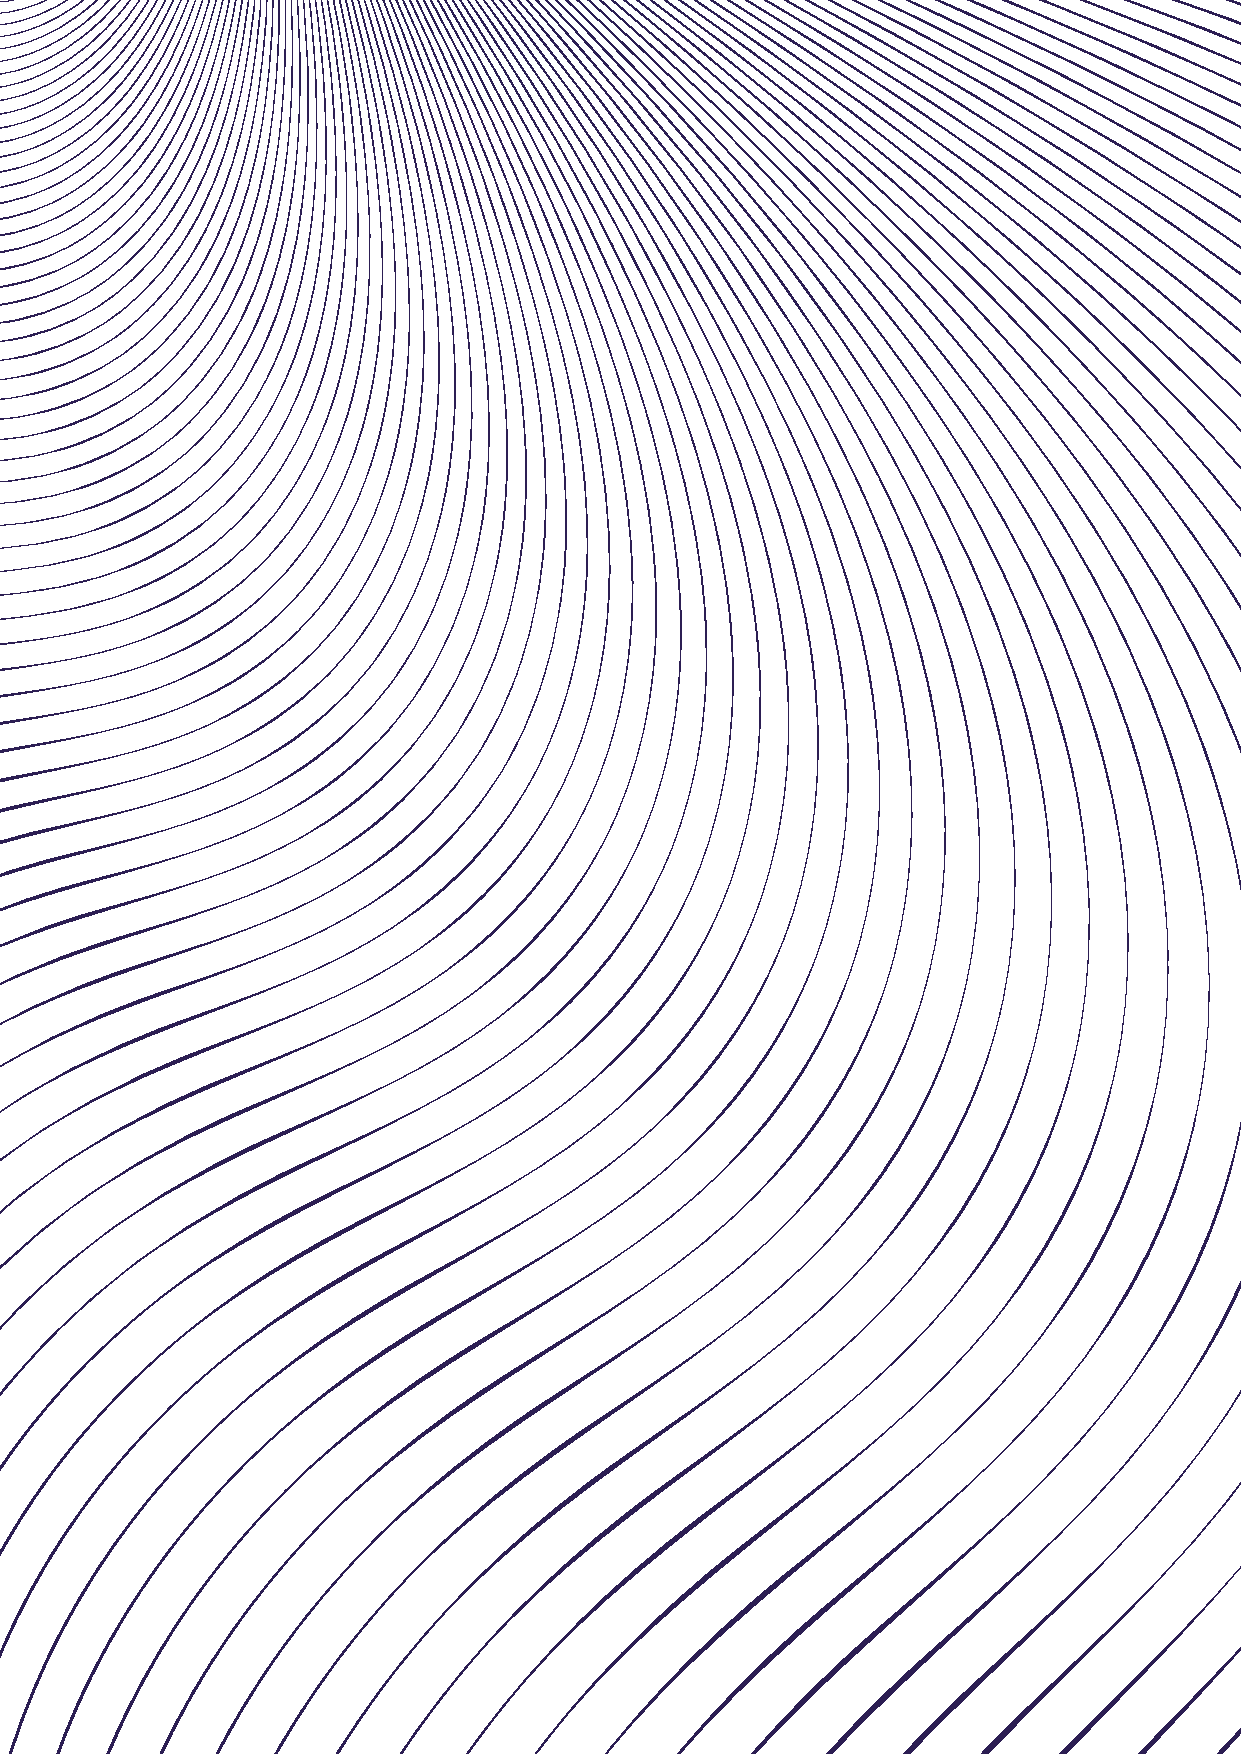
\includegraphics[width=\paperwidth,height=\paperheight]{aaugraphics/aau_waves.pdf}};
 %background waves end 

  \fboxsep0pt\colorbox{aaublue}

   \vfill% add spacing 
    \noindent

    {\colorbox{aaublue}{\begin{tabular}{@{}p{\textwidth}@{}}% Adding box
    \color{white}
     \begin{center}
     \Huge{\textbf{Characterizing passive components}}
     \end{center}
     \vspace{0.2cm}
    \begin{center}
     {\Large
        Joachim R.B. Andersen\\
        Jakob F. Thiesen\\
      }
     \vspace{0.4cm}
     {\large
       Bachelor of Engineering of Electronics, 7th semester, 2024
     }
    \end{center}
    \vspace{0.2cm}
   \end{tabular}}}
 
   \vfill %spacing
   \begin{center} %add circle logo
     
\includegraphics[width=0.2\paperwidth]{aaugraphics/aau_logo_circle_en.pdf}
   \end{center}
 \end{titlepage}
 \clearpage

\selectlanguage{english}
\pdfbookmark[0]{Danish title page}{label:titlepage_en}

\aautitlepage{%
  \englishprojectinfo{
     %title
     Design of a Spectral Impedance Analyzer for Passive Elements
  }{%
    Designing and constructing an Impedance Analyzer%theme
  }{%
    Fall Semester 2024 %project period
  }{%
    Group 771 - EIT7% project group
  }{%
    %list of group members
    Joachim R.B. Andersen\\
    Jakob F. Thiesen
    
  }{%
    %list of supervisors
    %The omnissiah
    Troels B. Sørensen
  }{%
    2 % number of printed copies
  }
  { %number of pages in the main matter
   A lot
  }
  {%
    \today % date of completion
  }%
}{%department and address
  \textbf{Electronics and IT}\\
  Aalborg University\\
  \href{http://www.aau.dk}{http://www.aau.dk}
}{% the abstract
This project focused on the development of a cost-effective impedance analyzer specifically designed for the characterization of passive components such as capacitors and inductors.

The initial phase involved a problem analysis to identify the target market, assess existing impedance analyzers in terms of functionality, cost, and accessibility. Our analysis revealed a gap in the market for a device that combines key features of high-end instruments at a price point accessible to a broader audience, including hobbyists, educational institutions, and small-scale enterprises.

Based on this, we developed an impedance analyzer with specifications aimed at delivering high performance at a reduced cost. The design phase included defining critical system requirements, followed by a lengthy hardware, and software, design phase and culminating in the creation of a PCB. The PCB was subsequently tested to validate the projects functionality against the set specifications.

The resulting impedance analyzer demonstrated capabilities for measuring impedance across a wide frequency range and is suitable for characterizing important parameters of passive components. This project offers a practical solution for affordable impedance measurement but also contributes to making advanced electronic testing equipment more accessible to the general public.
}

\thispagestyle{empty}
\chapter*{Preface}\label{ch:preface}

This report was written during the 7th semester of the Bachelor of Engineering of Electronics at Aalborg University in the 2024 fall semester and documents the work being done as part of the bachelors project.

The topic of this project is to analyze what an impedance analyzer is, how it works, why it is expensive and if it is possible to design and construct a cheaper, but still capable, instrument to do the same job as the commercially available instruments.

This report is confidential and the authors request that this document not be shared or distributed in any way without permission from the authors.

\vspace{\baselineskip}\hfill Aalborg University, \today


\begin{minipage}[b]{0.45\textwidth}
 \centering
 {\setstretch{0.1}
 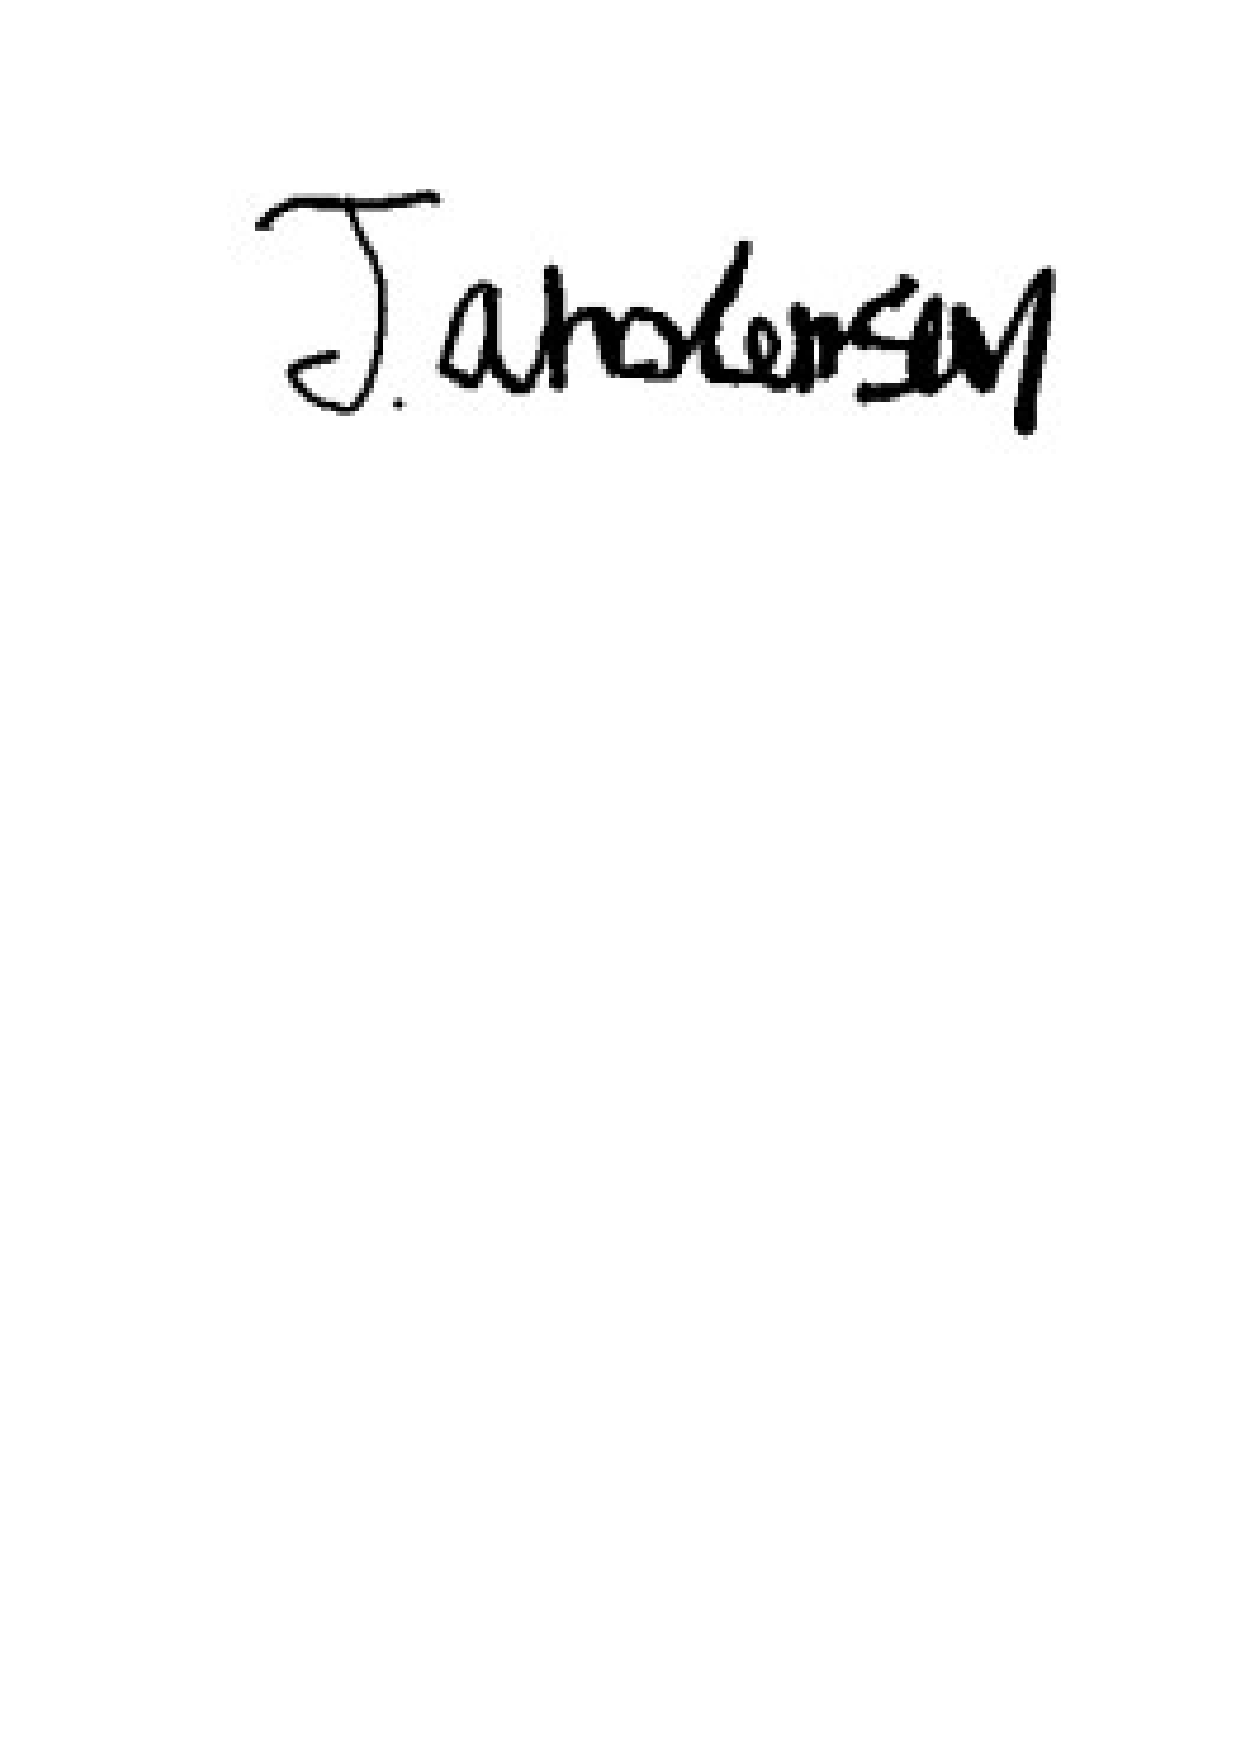
\includegraphics[clip, trim=0 600 0 0, width=0.8\textwidth]{Formalia/Figures/Jsig.pdf}
 \rule{\textwidth}{0.5pt}\\}
 Joachim R.B. Andersen\\
 {\footnotesize <jander20@student.aau.dk>}
 {\footnotesize <j.rixen@outlook.dk>}
\end{minipage}
\hfill
\vspace{5pt}
\begin{minipage}[b]{0.45\textwidth}
 \centering
 {\setstretch{0.1}
 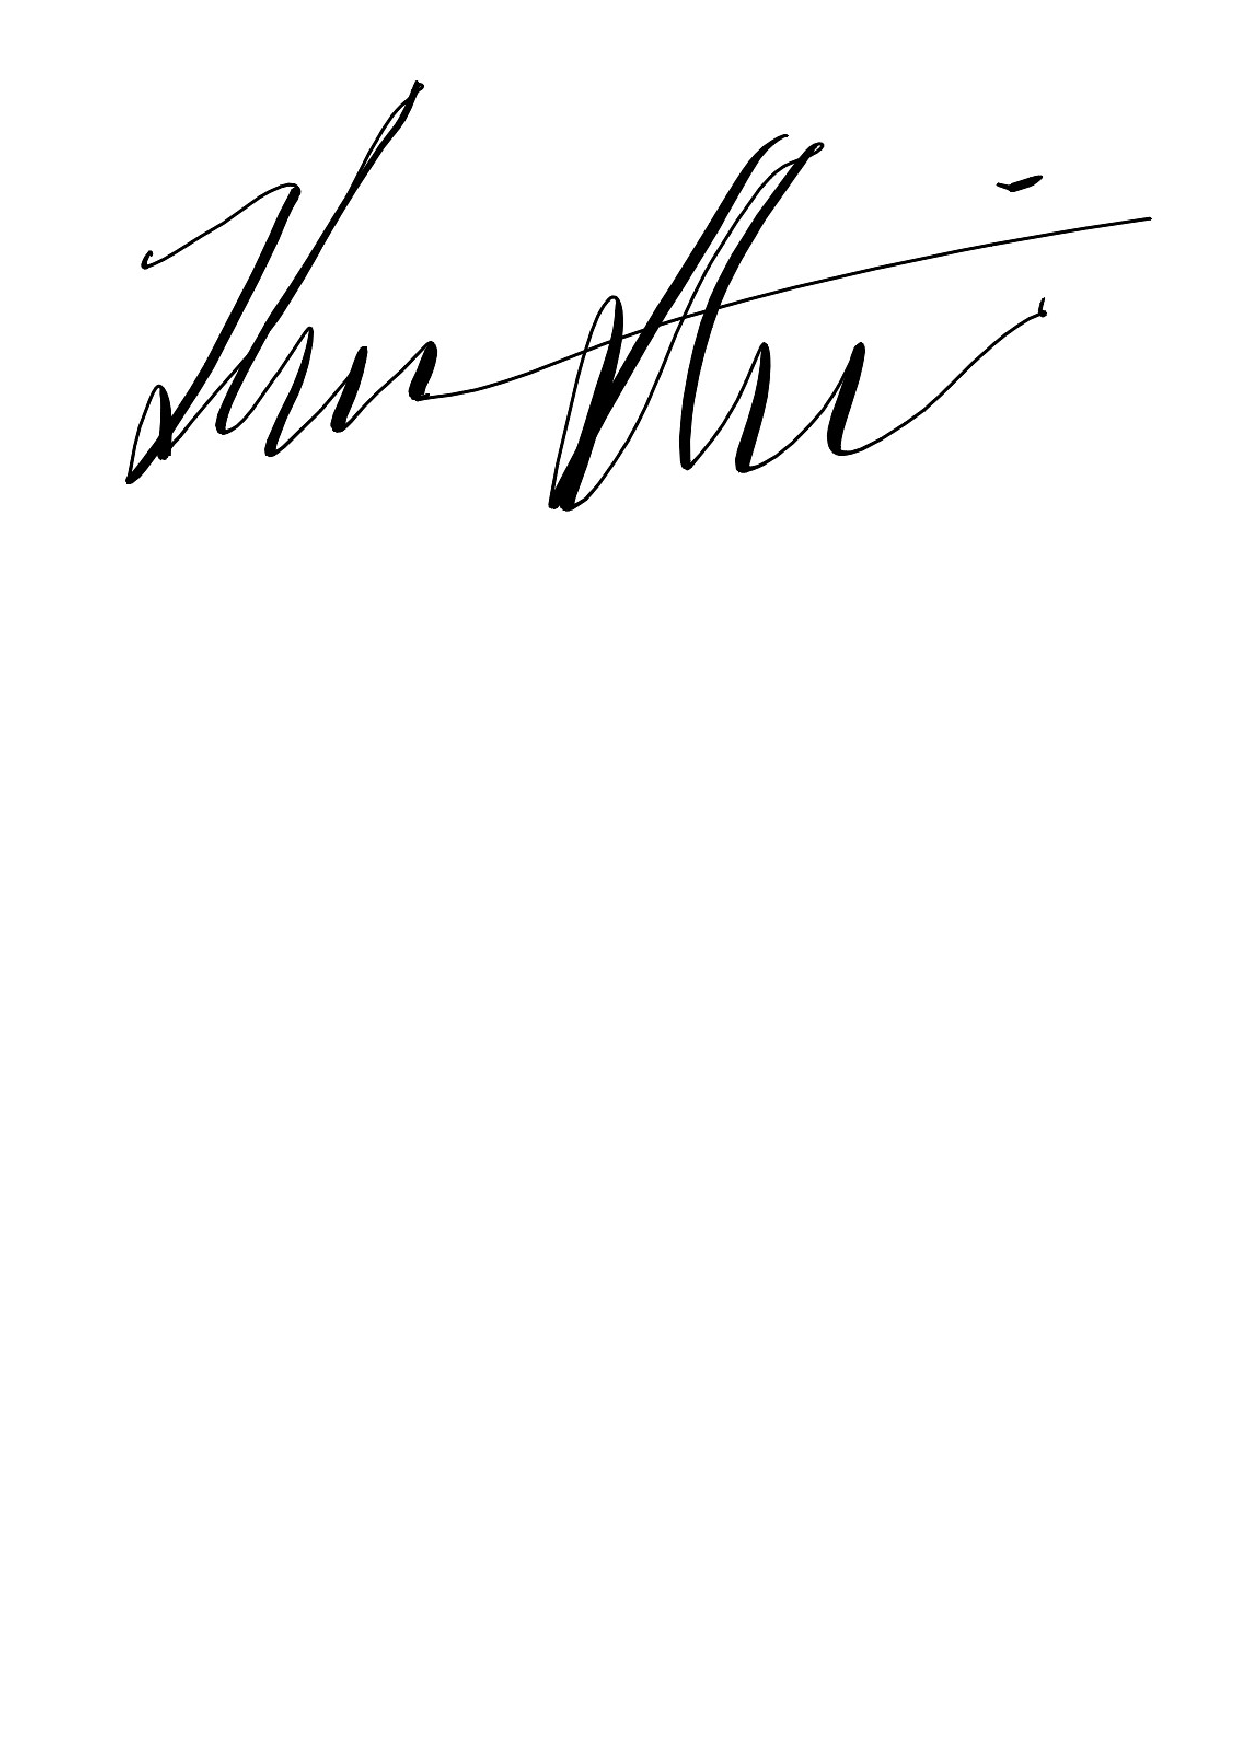
\includegraphics[clip, trim=0 575 0 0, width=0.8\textwidth]{Formalia/Figures/JakSig.pdf}
 \rule{\textwidth}{0.5pt}\\}
 Jakob F. Thiesen\\
 {\footnotesize <jfth21@student.aau.dk>}
 {\footnotesize <jakob.thiesen97@gmail.com>}
\end{minipage}


\tableofcontents
\clearpage
%


\section{References, labels and abbreviations}
% Please add the following required packages to your document preamble:
% \usepackage[table,xcdraw]{xcolor}
% If you use beamer only pass "xcolor=table" option, i.e. \documentclass[xcolor=table]{beamer}
\begin{table}[H]
\begin{tabular}{|l|l|}
\hline

Section type  & Reference/Label name \\ \hline
Chapter       & ch:name                  \\ \hline
Section       & sec:name                  \\ \hline
Subsection    & subsec:name               \\ \hline
Subsubsection & subsubsec:name           \\ \hline
Figure        & fig:name                  \\ \hline
Table         & tab:name                  \\ \hline
Equation      & eq:name                   \\ \hline
code snippets & snip:name                 \\ \hline
Appendix      & app:name                  \\ \hline
Bibliography  & bib:name\_addition\_another\_addition                \\ \hline
\end{tabular}
\end{table}
\section{Figures and tables}
\subsection{2 by x table}
\begin{table}[H]
\begin{tabular}{|l|l|}
\hline

        &       \\ \hline
        &       \\ \hline
        &       \\ \hline
\end{tabular}
\end{table}

\subsection{3 by x table}
\begin{table}[H]
\begin{tabular}{|l|l|l|}
\hline

        &       &       \\ \hline
        &       &       \\ \hline
        &       &       \\ \hline
\end{tabular}
\end{table}
\subsection{colored 3 by x table}
\begin{table}[H]
\begin{tabular}{|l|l|l|}
\hline
 
&  &  \\ \hline
 &  &  \\ \hline
 &  &  \\ \hline
\end{tabular}
\end{table}

\subsection{Figure figure}
Inserting figures of type: PDF, JPEG, JPG, PNG
\begin{figure}[H]
    \centering
    
\includegraphics[width=0.5\textwidth]{aaugraphics/aau_logo_circle_en.pdf}
    \caption{Caption}
    \label{fig:enter_label2}
\end{figure}

\subsection{SVG figure}
\begin{figure}[H]
    \centering
    \includesvg[width=0.3\textwidth]{Sections/1_Introduction/figures/Smiley.svg}
    \caption{ SVG smiley. He is happy be cause the file size is small but the resolution is high}
    \label{fig:enter_label1}
\end{figure}

\section{Unit and equations}
Examples of how to use units and different equations
\subsection{SI units}

\subsection{Equations}
\paragraph*{numerated equation:}
In equation \ref{ex:eq1} how to set up a enumerated equation can be seen.
\begin{equation}\label{ex:eq1}
    K_T = \frac{\tau}{I_a}
\end{equation}
\begin{conditions}
    K_T     & motor constant\\
    \tau    & the torque the motor produces\\
    I_a     & the current the motor draws\\
\end{conditions}


\paragraph*{unnumerated equation:}
In equation \ref{ex:eq2} how to set up an unenumerated equation can be seen. The reference however is changed to the nearest reference-able title object. Always try to add a reference to the equation, it might come in handy.
\begin{equation*}\label{ex:eq2}
    K_T = \frac{\tau}{I_a}
\end{equation*}
\begin{conditions}
    K_T     & motor constant\\
    \tau    & the torque the motor produces\\
    I_a     & the current the motor draws\\
\end{conditions}

\paragraph*{How to do math in latex}
If the table below is not fulfilling:
\url{https://www.cmor-faculty.rice.edu/~heinken/latex/symbols.pdf}

\begin{table}[H]
\centering
\renewcommand{\arraystretch}{1.5}
\begin{tabular}{|l |c|l|} \hline   
addition & + & + \\ \hline 
subtraction & - & - \\ \hline 
multiplication & $\cdot$ & \textbackslash{cdot} \\ \hline 
division & $\frac{num}{denom}$ & \textbackslash{frac\{num\}\{denom\}} \\ \hline 
powers & $a^{b+c}$ & a\^ \space\{b+c\}\\ \hline 
square root & $\sqrt{a+b} $ & \textbackslash{sqrt(a+b)} \\ \hline 
summation & $\sum $ & \textbackslash{sum} \\ \hline 
integration & $\int$ & \textbackslash{}int \\ \hline 
2x int & $\iint$ & \textbackslash{}iint \\ \hline 
3x int & $\iiint$ & \textbackslash{}iiint \\ \hline 
differentiation & $\dot{a}$ & \textbackslash{Ddot\{a\{}\\ \hline 
2x diff & $\Ddot{a}$ & \textbackslash{Ddot\{a\{}\\ \hline 
vector notation & $\overline{\rm AB}$  & \textbackslash{}overline\{\rm AB\}  \\ \hline

\end{tabular}

\end{table}




% Introduction
\chapter{Introduction} \label{ch:Introduction}
Among hobbyists, tinkerers and smaller companies, there is a need to characterize the most basic one-port electronic devices such as capacitors, inductors and resistors. Resistors can be bought, relatively, cheaply while still having a high degree of accuracy. Inductors and capacitors, however, often have significantly looser tolerances. Another limitation of reactive devices is the level of detail provided in their datasheets. Often values such as ESR or phase angle are not stated, nor their frequency or bias voltage stability. These parameters can be crucial for a designer when engineering an accurate, reliable and predicable circuit.

These component parameters can be measured, or at least somewhat estimated by the means of a rather large and complicated test-setup, involving both signal generators and oscilloscopes. The amount of steps required to take measurements such as these makes it prone to human errors and errors inherent to the test setup. As an added constraint; the test procedure is tedious to perform and, because of the limited range of the setup, the results can be inaccurate, especially at higher frequencies.

Professional test equipment for exactly this purpose is available on the market and are known in the industry as LCR meters. These devices come in a broad range of measurement capabilities and frequency ranges. Whilst these devices are available, the LCR meters with both good accuracy, flexible capabilities and high frequency ranges are prohibitively expensive and beyond the reach of most individuals, and small companies. These issues leads to the initial problem statement of this project.

“Why are these high-end LCR meters so expensive? Is it possible to estimate the characteristics of a passive device in a more economical way than what is present on the market today?”


% Problem Analyse
\chapter{Problem Analysis} \label{ch:ProblemAnalysis}
This section seeks to explain how passive components can, generally, be characterized and what instruments are commercially available to do it. The section will also discuss which requirements both professional and individuals may have for an LCR meter and what a reasonable price point may be for an individual.
\section{Measuring reactive components} \label{sec:MeasureReactiveComponents}

testfafafa
\section{Commercial Instruments} \label{sec:CommercialImpedanceMeasurement}
Most of the major manufacturers of test equipment, such as Keysight Technologies, Rohde \& Schwarz, Tektronix and others produce a range of instruments for characterizing passive components. This section will sample a few of these to research their capabilities, to indicate what a user might want and need. The instruments are chosen based on their perceived price range. 

LCR meters typically come in two different form factors, one is a handheld device, much like a regular multimeter, while the other is a benchtop instrument. The handheld LCR meters, like the Keysight U1733C\cite{KeysightU1733C}, shown in figure \ref{fig:2_2_U1733C}.
\begin{figure}[H]
    \centering
    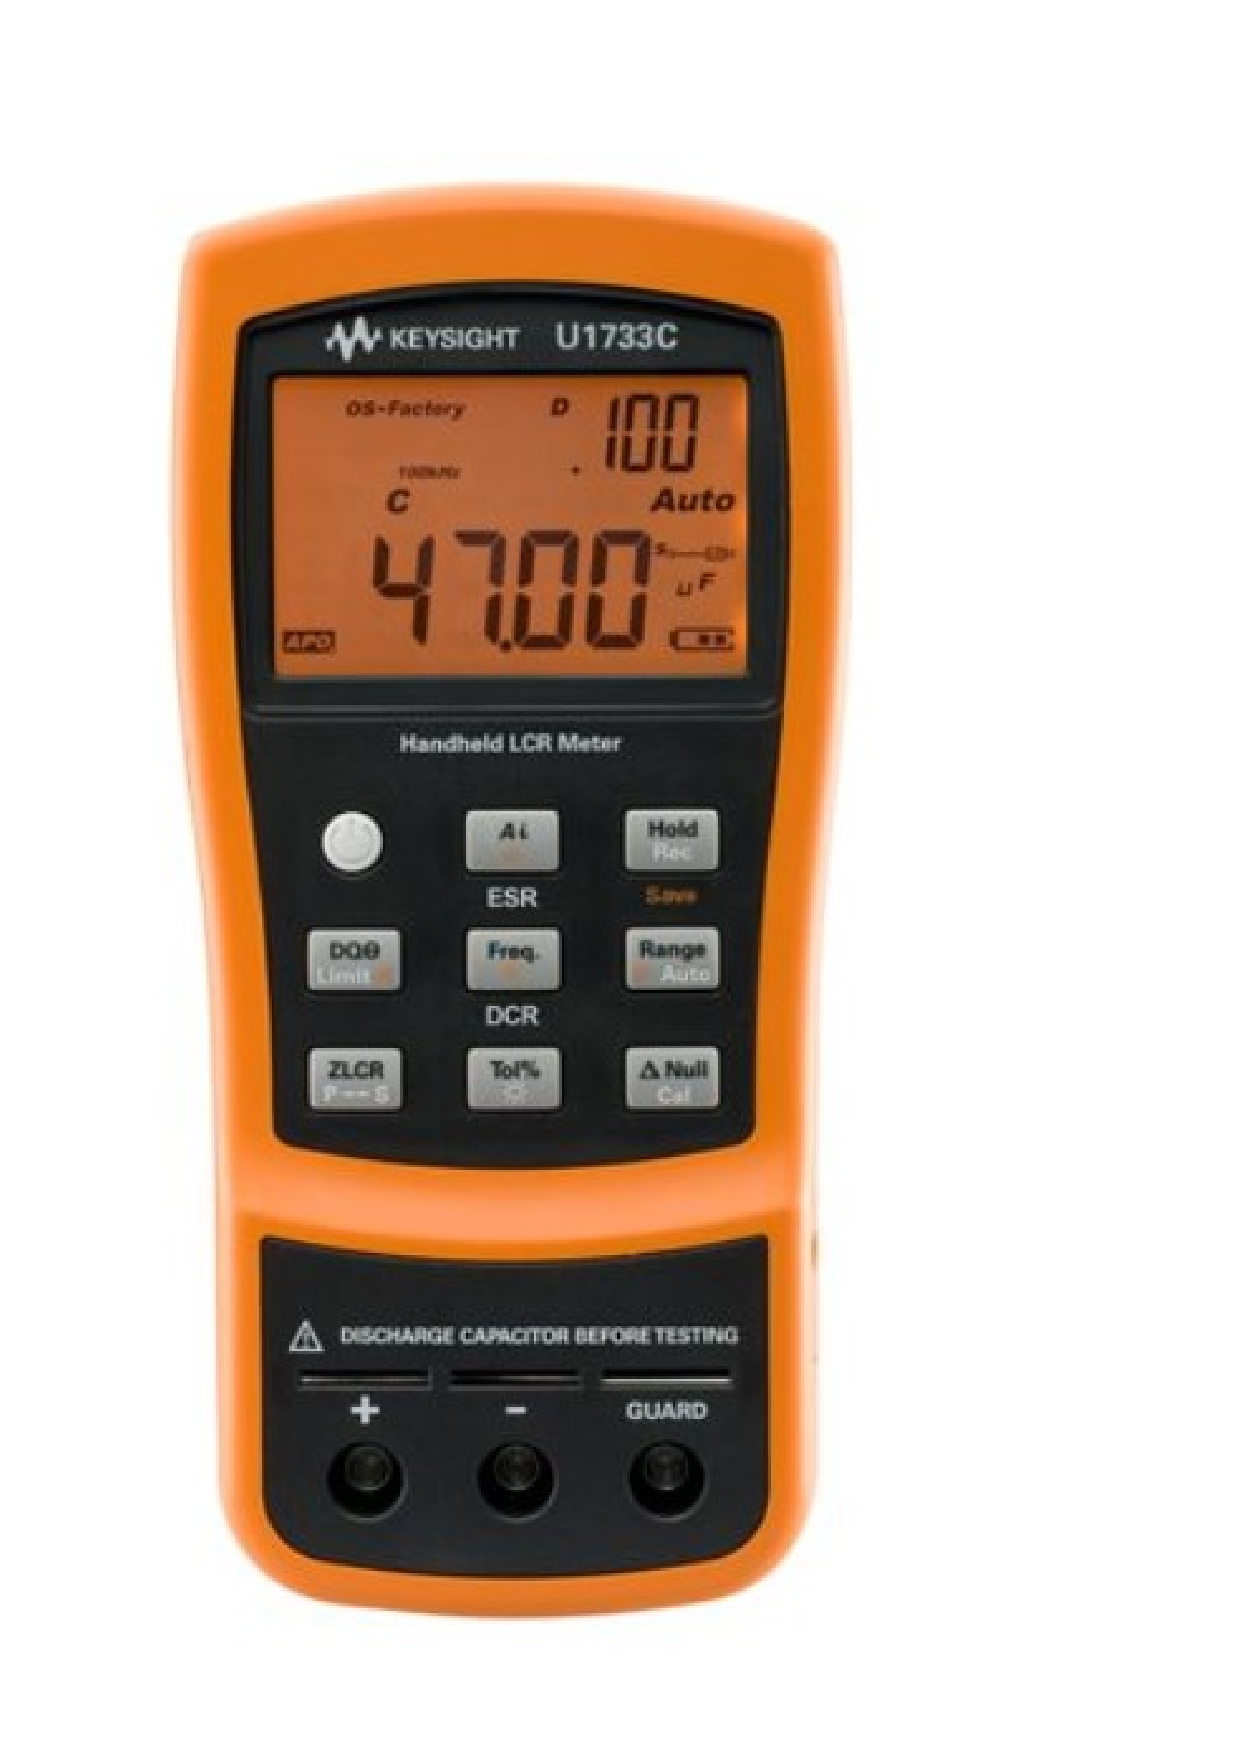
\includegraphics[clip, trim=0 50 0 50, width=0.5\textwidth]{Sections/2_ProblemAnalysis/FIgures/KeysightU1733C.pdf}
    \caption{A handheld Keysight U1733C LCR meter.\cite{KeysightU1733C}}
    \label{fig:2_2_U1733C}
\end{figure}
The U1733C shown on \ref{fig:2_2_U1733C} is meant for, primarily, troubleshooting and repair work and not electronics development purposes, while it is affordable at about 550€, it has limited capabilities. It can measure all the basic parameters such as capacitance, inductance, ESR and display all the derived quantities like dissipation and quality factor, see section \refq{subsec:DerivedQuantities} for further explanation. Numerically, however it can only take these measurements at a pre-determined set of test frequencies in the range \SI[]{100}{\hertz} to \SI[]{100}{\kilo\hertz} with measurement accuracy weaning off in both ends of the impedance range, and at higher frequencies.

Table \refq{tab:2_3_AccuracyTab_U1733C} shows the accuracy the impedance magnitude for the U1733C at the high and low end of the impedance ranges, as well as over a range of frequencies. Table \refq{tab:2_3_PhaseAccuracyTab_U1733C} shows the corresponding phase angle accuracy at the same impedances and frequencies. It clearly shows that at the extremes of impedance the accuracy degrades.

\begin{table}[H]
  \begin{tabular}{|m{6.3em}|m{6.3em}|m{6.3em}|m{6.3em}|m{6.3em}|}
  \hline
   Frequency / \nl Applied \nl Impedance & \SIQ{100}{\hertz} & \SIQ{1}{\kilo\hertz} & \SIQ{10}{\kilo\hertz} & \SIQ{100}{\kilo\hertz} \\ \hline
  \SIQ{1}{\ohm}    &   \SIQ{1.2}{\%}   &   \SIQ{1.2}{\%}    &   \SIQ{1.2}{\%}     &   \SIQ{1.5}{\%}      \\ \hline
  \SIQ{10}{\ohm}   &   \SIQ{0.78}{\%}     &  \SIQ{0.78}{\%} & \SIQ{0.78}{\%}  & \SIQ{0.78}{\%}    \\ \hline
  \SIQ{1}{\kilo\ohm}   &   \SIQ{0.23}{\%}     & \SIQ{0.23}{\%}  &  \SIQ{0.23}{\%}  & \SIQ{0.55}{\%} \\ \hline
  \SIQ{100}{\kilo\ohm} &   \SIQ{0.55}{\%}     &  \SIQ{0.55}{\%}  & \SIQ{0.55}{\%}   & \SIQ{0.78}{\%}  \\ \hline
  \SIQ{100}{\mega\ohm} &   \SIQ{6.8}{\%}     &   \SIQ{6.8}{\%}  &  NA   &   NA  \\ \hline
  \end{tabular}
  \caption{Table of selected impedance measurement accuracy of a U1733C. It can be seen that the accuracy degrades at higher frequencies and at the extreme ends of the impedance capabilities.}
  \label{tab:2_3_AccuracyTab_U1733C}
  \end{table}


  \begin{table}[H]
    \begin{tabular}{|m{6.3em}|m{6.3em}|m{6.3em}|m{6.3em}|m{6.3em}|}
    \hline
     Frequency / \nl Applied \nl Impedance & \SIQ{100}{\hertz} & \SIQ{1}{\kilo\hertz} & \SIQ{10}{\kilo\hertz} & \SIQ{100}{\kilo\hertz} \\ \hline
    \SIQ{1}{\ohm}    &   \SIQ{0.69}{\degree} &   \SIQ{0.69}{\degree} &   \SIQ{0.69}{\degree}  &  \SIQ{0.86}{\degree}  \\ \hline
    \SIQ{10}{\ohm}   &   \SIQ{0.45}{\degree}     &  \SIQ{0.45}{\degree} & \SIQ{0.45}{\degree}  & \SIQ{0.45}{\degree}  \\ \hline
    \SIQ{1}{\kilo\ohm}   &  \SIQ{0.13}{\degree}  & \SIQ{0.13}{\degree}  &  \SIQ{0.13}{\degree}  & \SIQ{0.32}{\degree} \\ \hline
    \SIQ{100}{\kilo\ohm} &   \SIQ{0.32}{\degree} &  \SIQ{0.32}{\degree} & \SIQ{0.32}{\degree}  & \SIQ{0.45}{\degree}  \\ \hline
    \SIQ{100}{\mega\ohm} &   \SIQ{3.90}{\degree}     &   \SIQ{3.90}{\degree}  &  NA   &   NA  \\ \hline
    \end{tabular}
    \caption{Table of selected phase angle measurement accuracy of a U1733C. It can be seen that the accuracy degrades at higher frequencies and at the extreme ends of the impedance capabilities.}
    \label{tab:2_3_PhaseAccuracyTab_U1733C}
    \end{table}


The U1733C datasheet has similar charts for other measurements, but they follow a similar pattern of accuracy as capacitance where it becomes clear that the accuracy is worse in the higher ends of the range. The accuracy is listed as a $\%$ of range $ + n\cdot resolution$, so a measurement in the \SI[]{20}{\micro\farad} range will have an accuracy of $\pm \SI[]{1}{\micro\farad} + \SI[]{10}{\nano\farad} = \SIQ{1.01}{\micro\farad}$ at \SIQ{100}{\kilo\hertz}.

Rohde \& Schwarz has a benchtop line of LCR meters called the LCX line \cite{RSLCXLCRMeters}. These have tighter specifications for accuracy, a greater range and a more diverse set of displaying the measurements. They also come with a significantly higher price tag at 15000€ for a 500kHz bandwidth version. This LCR meter is shown on figure \ref{fig:2_2_RSLCX}.
\begin{figure}[H]
    \centering
    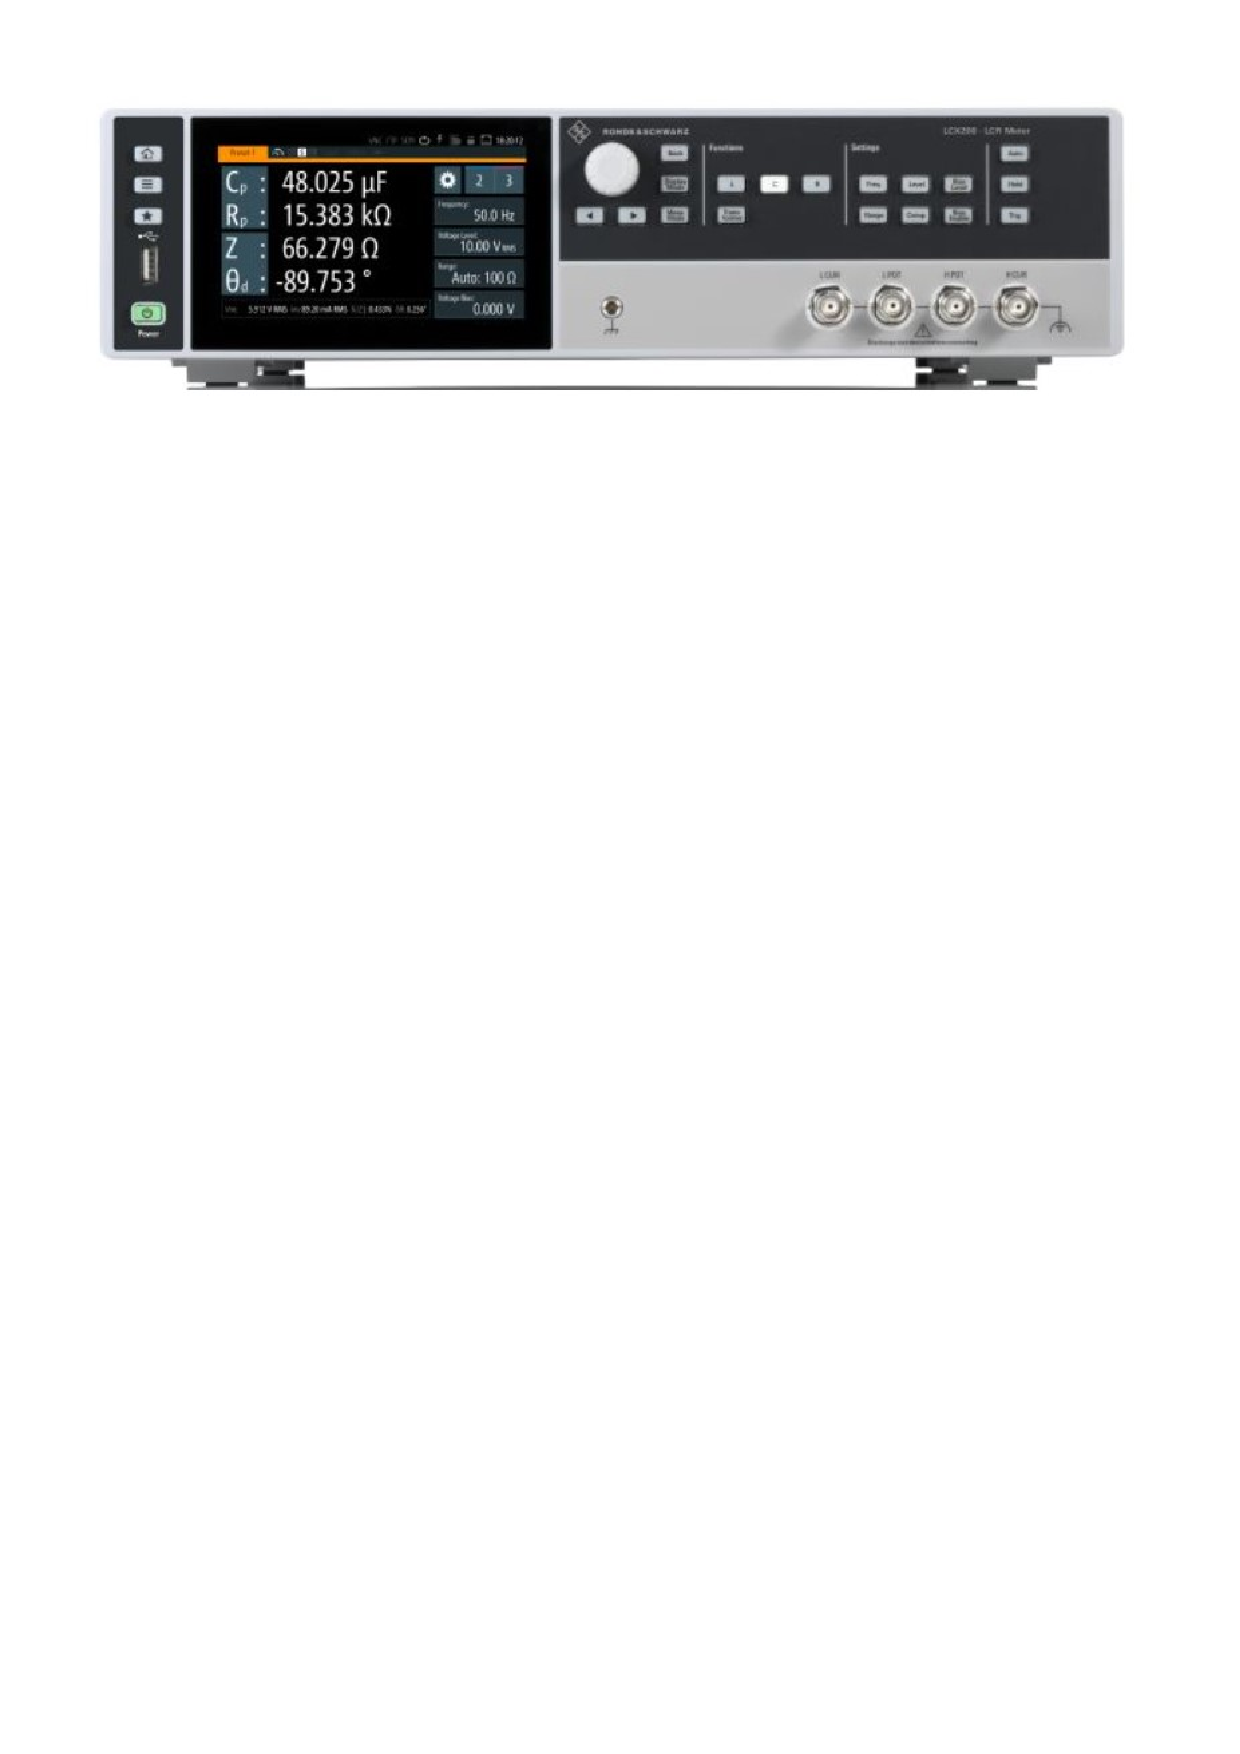
\includegraphics[clip, trim=0 630 0 50, width=1\textwidth]{Sections/2_ProblemAnalysis/FIgures/RSLCXLCR.pdf}
    \caption{A Rohde \& Schwarz LCX LCR meter featured a significantly greater bandwidth when compared to the U1733C, 4-wire kelvin measurements and greater ability to display the measurements.\cite{RSLCXLCRMeters}}
    \label{fig:2_2_RSLCX}
\end{figure}

The Rohde \& Schwarz LCX LCR meter is using kelvin bridge (4-wire) measurements.  This feature is often seen on higher end test equipment in order for the instrument to compensate for the parasitics introduced by the test instruments own test leads. The instrument can be triggered to take measurements externally and be controlled remotely over various network interfaces. The meter also has a sweep function in order to measure the impedance of the DUT over a series of frequency values and can display all the measurements numerically of graphically. Unlike the U1733C this meter is intended for electronic development purposes.

The Wayne-Kerr 6500B\cite{WayneKerr6500} series is a high-end impedance analyzer for demanding applications. The industry differentiates between \textit{LCR meters} and \textit{Impedance analyzers}. An LCR meter will display it's single point measurements numerically, while an impedance analyzer can do the same but is meant specifically for frequency sweeps and displaying the measurements on graphs. In other words, an impedance analyzer is a more advanced LCR meter. The Wayne-Kerr 6500B is shown on figure \ref{fig:2_2_WayneKerr6500B}. 
\begin{figure}[H]
    \centering
    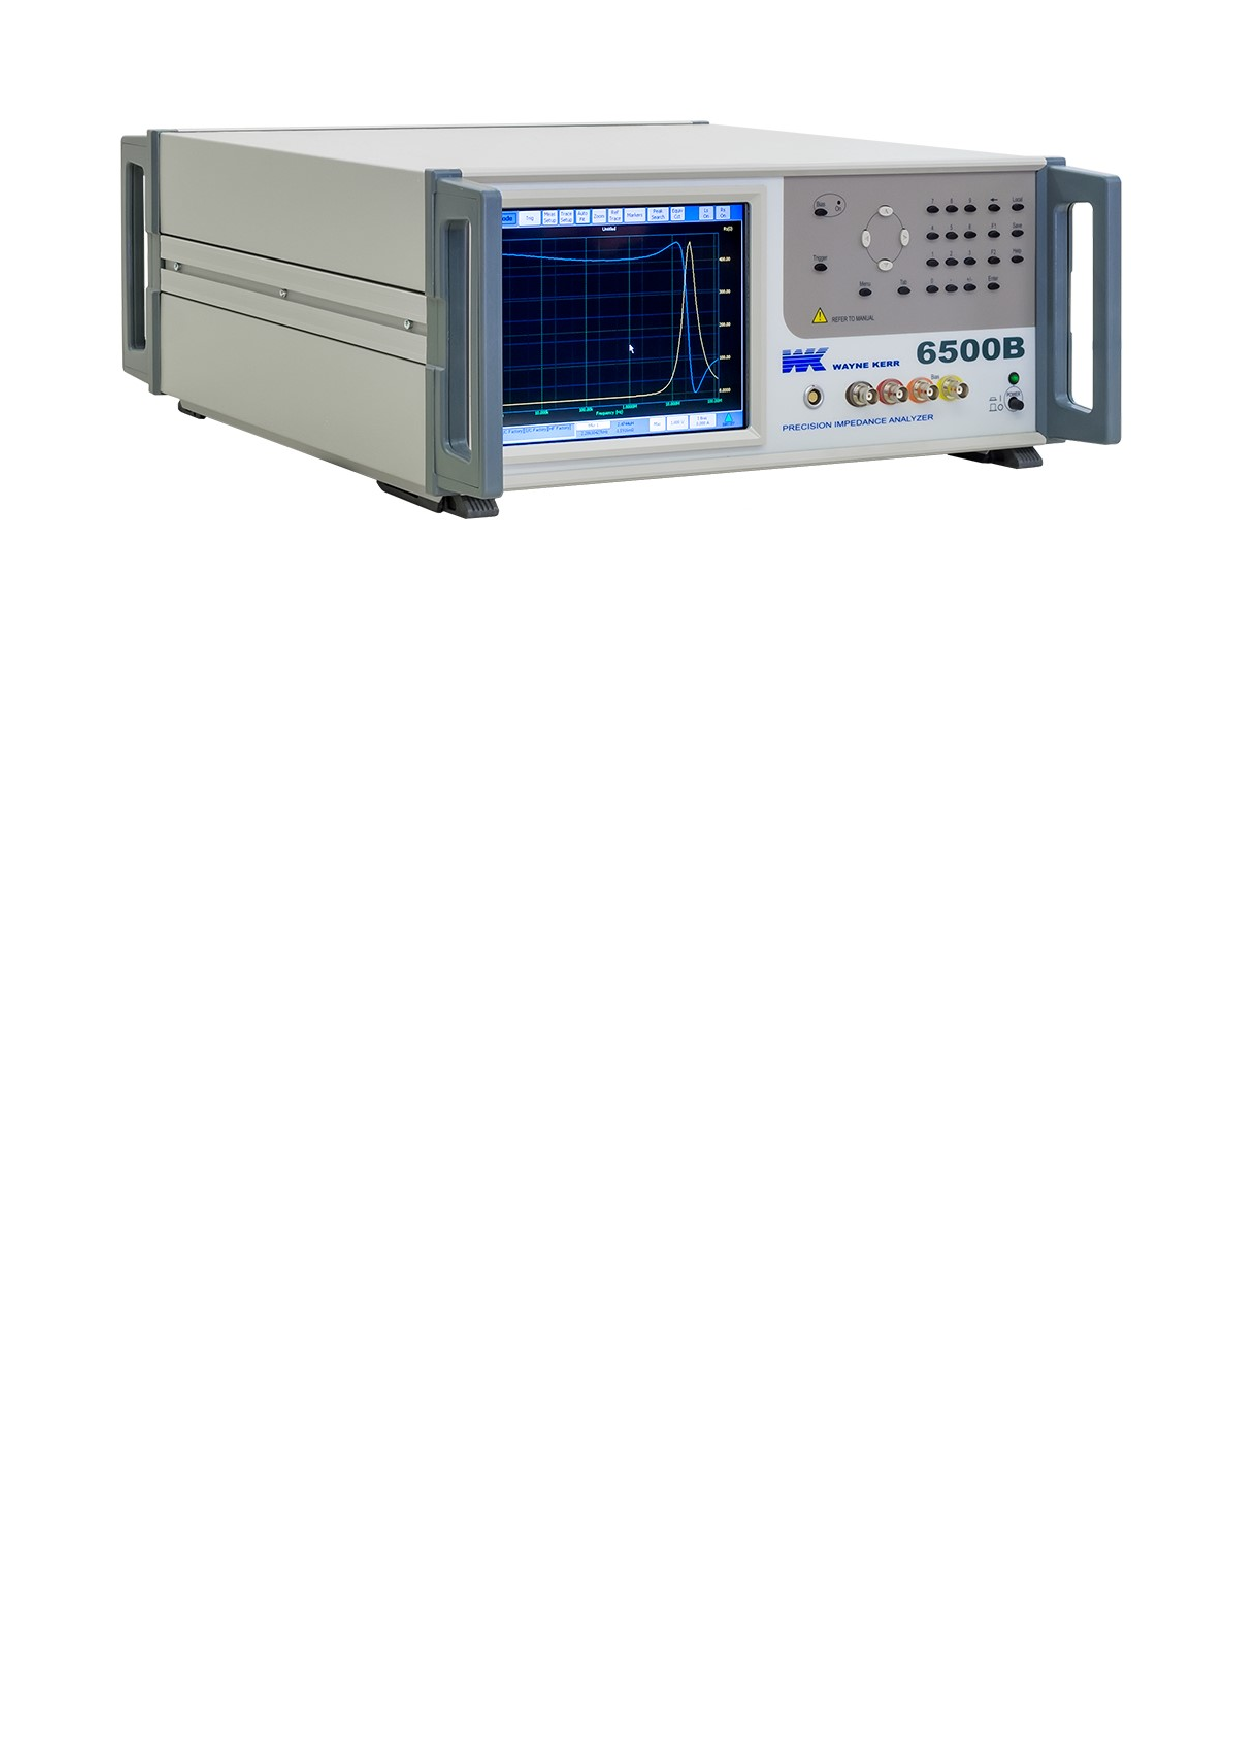
\includegraphics[clip, trim=0 550 0 50, width=1\textwidth]{Sections/2_ProblemAnalysis/FIgures/WayneKerrImpedanceAnalyzer.pdf}
    \caption{A Wayne-Kerr 6500B impedance analyzer. Note how it displays it's measurements graphically.}
    \label{fig:2_2_WayneKerr6500B}
\end{figure}
This impedance analyzer has a test frequency range of \SI[]{20}{\hertz} to \SI[]{120}{\mega\hertz} and has a test frequency resolution of \SI[]{100}{\micro\hertz} and Wayne-Kerr guarantees an accuracy of L, C and R measurements of $\pm 0.05$ \% across the entire frequency range putting this instrument in a different league from the ones previously shown. This impedance analyzer has adjustable DC bias as well, so bias stability can be measured as well. The impedance analyzer can display it's measurements on regular plots but can also show them in polar, or complex, form much like a network analyzer. The price of this instrument is listed as \textit{request quote} putting it far out of reach of even most smaller companies.

A few LCR meters and impedance analyzers were reviewed, there are many more but it would be impractical to list all of them. It was done in order to analyze what functionality they have. Their functionality and price points are closely related and a table has been made to break down the overall capabilities of each instrument. The results for this can be seen in table \ref{tab:2_3_CapabilityTab}.

\begin{table}[H]
  \begin{tabular}{|m{9.5em}|m{8em}|m{8em}|m{8em}|}
  \hline
    &   Keysight U1733C       & Rohde \&\newline Schwartz LCX      & Wayne-Kerr\newline 6500B                 \\ \hline
    Test frequency range      &  \SI[]{20}{\hertz} to \SI[]{100}{\kilo\hertz}$\mathbf{^1}$     &    DC-\SI[]{500}{\kilo\hertz},\newline \SI[]{1}{\hertz} steps   & \SI[]{20}{\hertz}-\SI[]{120}{\mega\hertz},\newline  \SI[]{100}{\micro\hertz} steps                                                  \\ \hline
    Basic accuracy$\mathbf{^2}$            &  [Z] 0.2\%\newline [$\phi$] $0.2$\%      & [Z] $\pm 0.05$\%\newline [$\phi$] $\pm 0.03$\degree       &[Z] $\pm 0.05$\%\newline [$\phi$] $\pm 0.0005$\degree                                                    \\ \hline
    Interface Type            &  Simple$\mathbf{^3}$\nl LCD, buttons    & Touchscreen & Touchscreen \\ \hline
    Measurement mode          &   2-wire    & 4-wire      & 4-wire                                  \\ \hline
    Auto ranging              &   Yes    & Yes      & Yes                                           \\ \hline
    Adj. DC Bias range        &   No    & \SIQ{40}{\volt}DC$\mathbf{^4}$      & $\pm$\SIQ{40}{\volt}DC           \\ \hline
    Frequency sweep           &   No    & Yes$\mathbf{^5}$      & Yes                               \\ \hline
    Data logging              &   No    & Yes      & Yes                                            \\ \hline
    Component binning         &   No    & Yes      & Yes                                            \\ \hline
    Graph data point          &   No    & Yes      & Yes                                            \\ \hline
    Complex plane plots       &   No    & No       & Yes                                             \\ \hline
    Network access            &   No    & Yes      & Yes                                  \\ \hline
    Price point               & <1000€   & 15000€   & Undisclosed                                    \\ \hline
  \end{tabular}
  \caption*{
    \raggedright
    $\mathbf{^1}$ The test frequencies for the U1733C are in pre-determined steps.\\
    $\mathbf{^2}$ \textit{Z} refers to impedance measurement accuracy. \textit{$\phi$} refers specifically to the phase measurement. The term \textit{basic accuracy} covers the minimum accuracy of L, C, R, ESR, D, Q measurements across the frequency range of the instrument.\\
    $\mathbf{^3}$ \textit{simple} refers to the instruments U/I being a few buttons and an LCD display as shown on figure \ref{fig:2_2_U1733C}.\\
    $\mathbf{^4}$ The Rohde \& Schwartz LCX DC bias setting is an extra software options that can be purchased\\
    $\mathbf{^5}$ The Rohde \& Schwartz LCX can do frequency sweeps if an extra software option is purchased.\\
  }
  \caption{A summary of the capabilties of the 3 instruments.}
  \label{tab:2_3_CapabilityTab}
\end{table}

As shown in table \ref{tab:2_3_CapabilityTab} there is a clear distinction in the level of features available at different price points and the major differentiator in their price is the instruments accuracy and test frequency range. The U1733C is affordable for most individuals but lacks a lot of the functions and range available at higher price brackets. The LCX and 6500B will have significantly more advanced hardware and a major difference between these two is there test frequency ranges. It is noteworthy how some of their features are due to them having more advanced software and interfaces. Some of these features could be made available in a lower price bracket with software alone. 



%\section{Commercial Instruments Capabilities} \label{sec:CommercialImpedanceAnalyzerCapabilities}
A few LCR meters and impedance analyzers were reviewed in section \ref{sec:CommercialImpedanceMeasurement}, there are many more but it would be impractical to list all of them, it was done in order to analyze what functionality they have. Their functionality and price points are, however, closely related. This section seeks to break down some of the functionality a customer could expect at certain price points. The results for this can be seen in table \ref{tab:2_3_CapabilityTab}.

\begin{table}[H]
  \begin{tabular}{|m{9.5em}|m{8em}|m{8em}|m{8em}|}
  \hline
    &   Keysight U1733C       & Rohde \&\newline Schwartz LCX      & Wayne-Kerr\newline 6500B                 \\ \hline
    Test frequency range      &  \SI[]{20}{\hertz} to \SI[]{100}{\kilo\hertz}$\mathbf{^1}$     &    DC-\SI[]{500}{\kilo\hertz},\newline \SI[]{1}{\hertz} steps   & \SI[]{20}{\hertz}-\SI[]{120}{\mega\hertz},\newline  \SI[]{100}{\micro\hertz} steps                                                  \\ \hline
    Basic accuracy$\mathbf{^2}$            &  [Z] 0.2\%\newline [$\phi$] $0.2$\%      & [Z] $\pm 0.05$\%\newline [$\phi$] $\pm 0.03$\degree       &[Z] $\pm 0.05$\%\newline [$\phi$] $\pm 0.0005$\degree                                                    \\ \hline
    Interface Type            &  Simple$\mathbf{^3}$\nl LCD, buttons    & Touchscreen & Touchscreen \\ \hline
    Measurement mode          &   2-wire    & 4-wire      & 4-wire                                  \\ \hline
    Auto ranging              &   Yes    & Yes      & Yes                                           \\ \hline
    Adj. DC Bias range        &   No    & \SIQ{40}{\volt}DC      & $\pm$\SIQ{40}{\volt}DC           \\ \hline
    Frequency sweep           &   No    & Yes$\mathbf{^4}$      & Yes                               \\ \hline
    Data logging              &   No    & Yes      & Yes                                            \\ \hline
    Component binning         &   No    & Yes      & Yes                                            \\ \hline
    Graph data point          &   No    & Yes      & Yes                                            \\ \hline
    Complex plane plots       &   No    & No       & Yes                                             \\ \hline
    Network access            &   No    & Yes      & Yes                                  \\ \hline
    Price point               & <1000€   & 15000€   & Undisclosed                                    \\ \hline
  \end{tabular}
  \caption*{
    \raggedright
    $\mathbf{^1}$ The test frequencies for the U1733C are in pre-determined steps.\\
    $\mathbf{^2}$ \textit{Z} refers to impedance measurement accuracy. \textit{$\phi$} refers specifically to the phase measurement. The term \textit{basic accuracy} covers the minimum accuracy of L, C, R, ESR, D, Q measurements across the frequency range of the instrument.\\
    $\mathbf{^3}$ \textit{simple} refers to the instruments U/I being a few buttons and an LCD display as shown on figure \ref{fig:2_2_U1733C}.\\
    $\mathbf{^4}$ The Rohde \& Schwartz LCX can do frequency sweeps if an extra software option is purchased.\\
  }
  \caption{Table to test captions and labels.}
  \label{tab:2_3_CapabilityTab}
\end{table}

There is a clear distinction in the level of features available at different price points. The U1733C is affordable for most individuals but lacks a lot of the functions available at higher price brackets. The LCX and 6500B will contain more advanced hardware and a major difference between these two is there test frequency ranges, but, it is noteworthy how some of their features are due to them having more advanced software and interfaces. Some of these features could be made available in a lower price bracket with software alone.  NOT USED ANYMORE
\section{Market demand} \label{sec:ProfessionalMarketDemand}
faf
\section{Problem Analysis Conclusion} \label{sec:probAnalConc}

%Here we put the conclusion of the problem analysis.
% Problem statement
\chapter{Problem Statement} \label{ch:ProblemStatement}

xD
% Technical Analysis
\chapter{Technical Analysis} \label{ch:TechnicalAnalysis}
This chapter will discuss what an \textit{impedance} is. The chapter will explain certain techniques for measuring the signals required to calculate the impedance and, once the impedance has been quantified, how to convert the impedance into the quantities of interest.




\section{Impedance analysis} \label{sec:ImpedanceAnalysis}
In order to measure, and analyze, an impedance it is important to have a clear definition of what impedance actually is. This sections will describe what an impedance is and how it can be used to analyze a device under test (DUT).

The impedance of a DUT, or circuit, is the devices ability to restrict the flow of alternating current and is the relationship between the current flowing through the DUT and the voltage across it. This can be visualized with a \textit{phasor} diagram. Phasors are vectors in the complex plane that represent sinewaves with a fixed amplitude and frequency. They are used to visualize phase shifts between different signals. For this analysis there will be voltage and current phasors as these can be used to find impedance phasors. Consider the case where the DUT is, mostly, capacitive in nature. In this case the current vector, $\bar i$, will lead the voltage vector $\bar v$ as shown on figure \ref{fig:4_1_CapPhasor}. \textit{lead} just means that the current has a positive phase shift relative to the voltage, if the opposite were true it would be \textit{lagging}.

\begin{figure}[H]
    \centering
    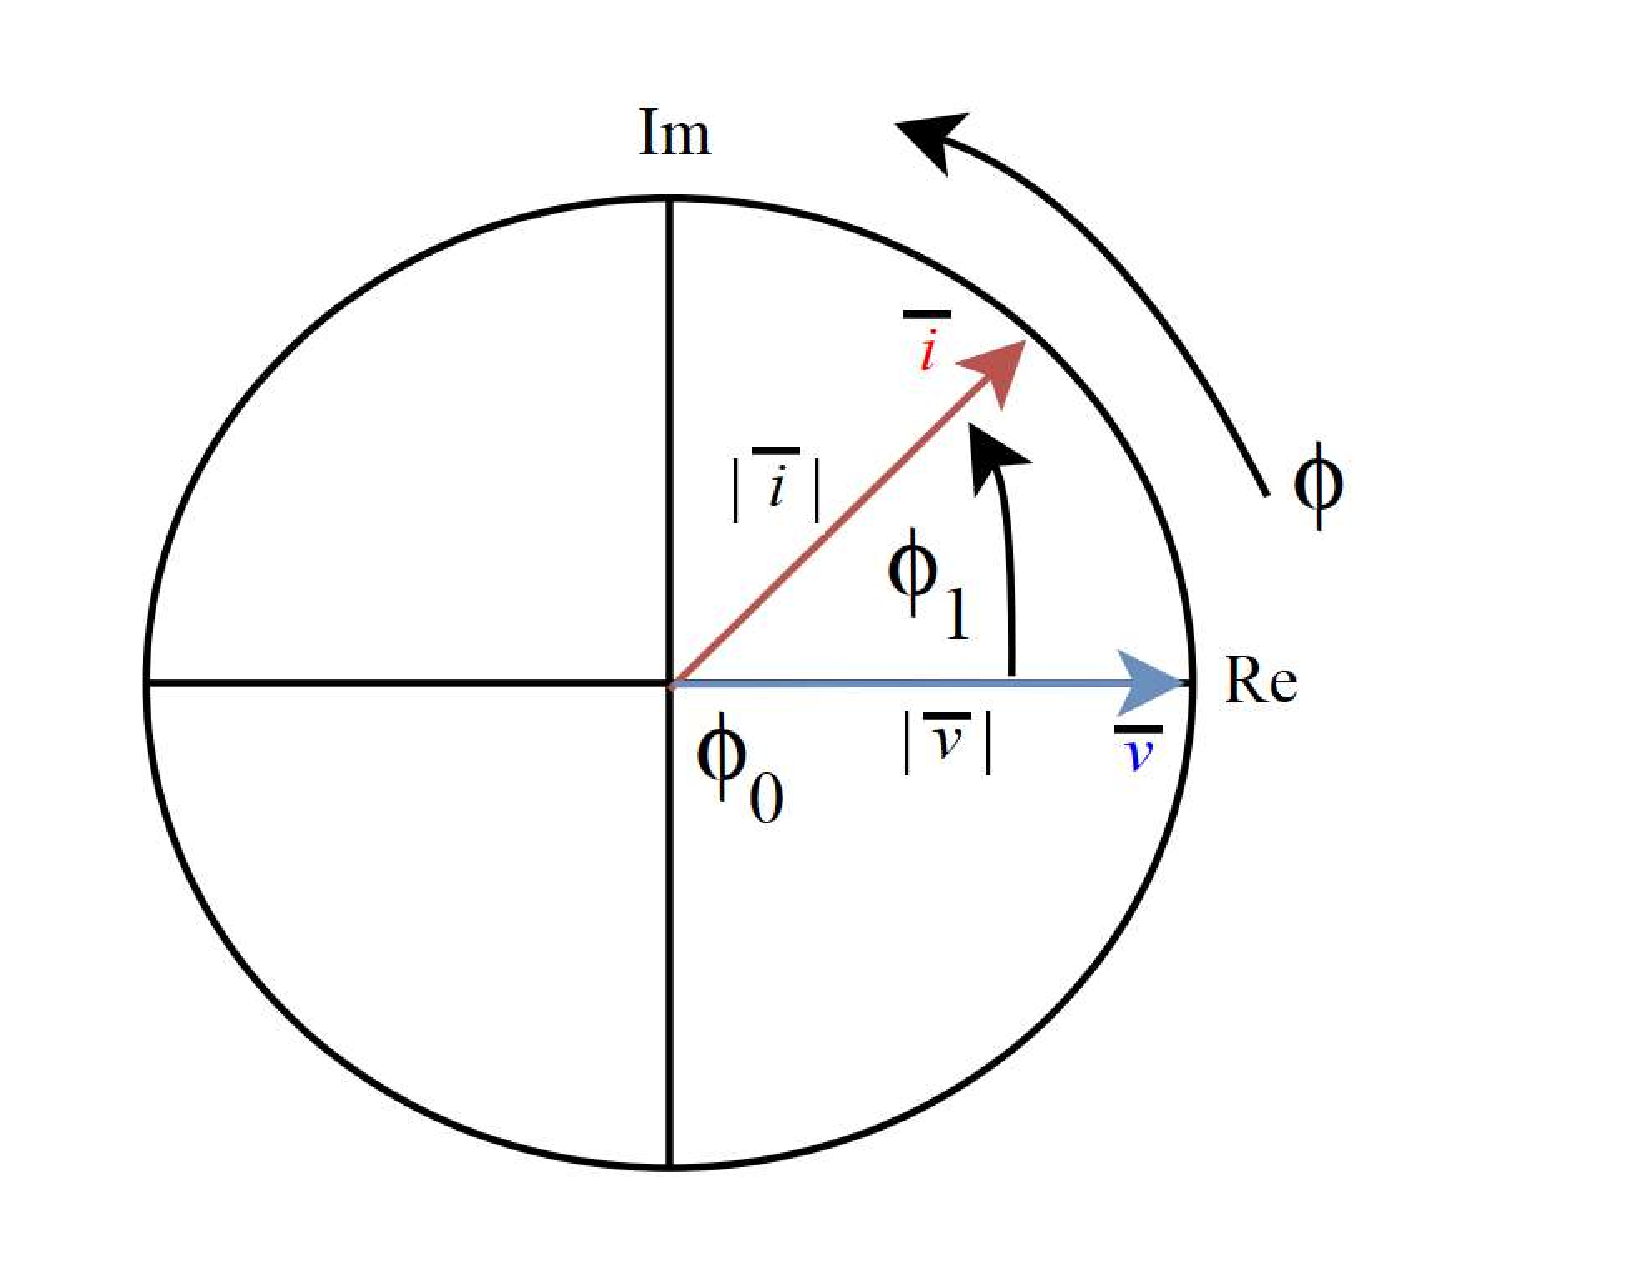
\includegraphics[clip, trim=0 0 0 0, width=0.60\textwidth]{Sections/4_TechnicalAnalysis/Figures/4_1_CapacitancePhasor.pdf}
    \caption{A capacitance causes the current $\bar i$ to lead the voltage $\bar v$. The black $\phi$ arrow signifies the positive direction of the coordinate system.}
    \label{fig:4_1_CapPhasor}
\end{figure}

The voltage vector, $\bar v$, with the phase $\phi_0 = 0$ relative to the real axis, will be the reference for the system because in impedance analyzers the input signal to the DUT will, most often, be a controlled voltage with a known phase and the DUT's phase will be relative to this input waveform. The phase difference $\Delta \phi = \phi_0 - \phi_1$ will correspond to the phase of the $\bar i$ current waveform. The phase of the reference waveform is $\phi_0 = 0$ and this gives the phase of $\bar i$ as shown in eq \ref{eq:4_1_CapPhase}.

\begin{equation}\label{eq:4_1_CapPhase}
    \Delta \phi = \phi_1 - \phi_0=\phi_1 \bigg\rvert_{\phi_0 = 0}
\end{equation}

The impedance of a DUT is the relationship between the voltage and current phasors as shown in equation \ref{eq:4_1_Impedance}.
\begin{equation}\label{eq:4_1_Impedance}
    \bar Z_c = \frac{|\bar v| [cos(\phi_0) +j\cdot sin(\phi_0)]}{|\bar i| [cos(\Delta \phi) +j\cdot sin(\Delta \phi)]}
\end{equation}

Using $\phi_0 = 0$ and $\Delta \phi = \phi_1$ in equation \ref{eq:4_1_Impedance} gets equation \ref{eq:4_1_CapImpedance2}. The numerator reduces to $|\bar v|$ as $cos(0) =1$ and $sin(0) = 0$.
\begin{equation}\label{eq:4_1_CapImpedance2}
    \bar Z_c = \frac{|\bar v|}{|\bar i| [cos(\phi_1) +j\cdot sin(\phi_1)]}
\end{equation}

Applying Eulers formula, and the reciprocal, to eq \ref{eq:4_1_CapImpedance2} gives the final expression for the impedance of a capacitive DUT shown in eq \ref{eq:4_1_CapImpedance4}.
\begin{equation}\label{eq:4_1_CapImpedance4}
    \bar Z_c = \frac{|\bar v|}{|\bar i|} \cdot \mathrm e^{-j\phi_1} = |\bar Z| \cdot \mathrm e^{-j\phi_1} 
\end{equation}
Plotting the impedance vector of a DUT dominated by a capacitance will give a vector pointing into the 4th quadrant as shown in figure \ref{fig:4_1_CapImpedance}.
\begin{figure}[H]
    \centering
    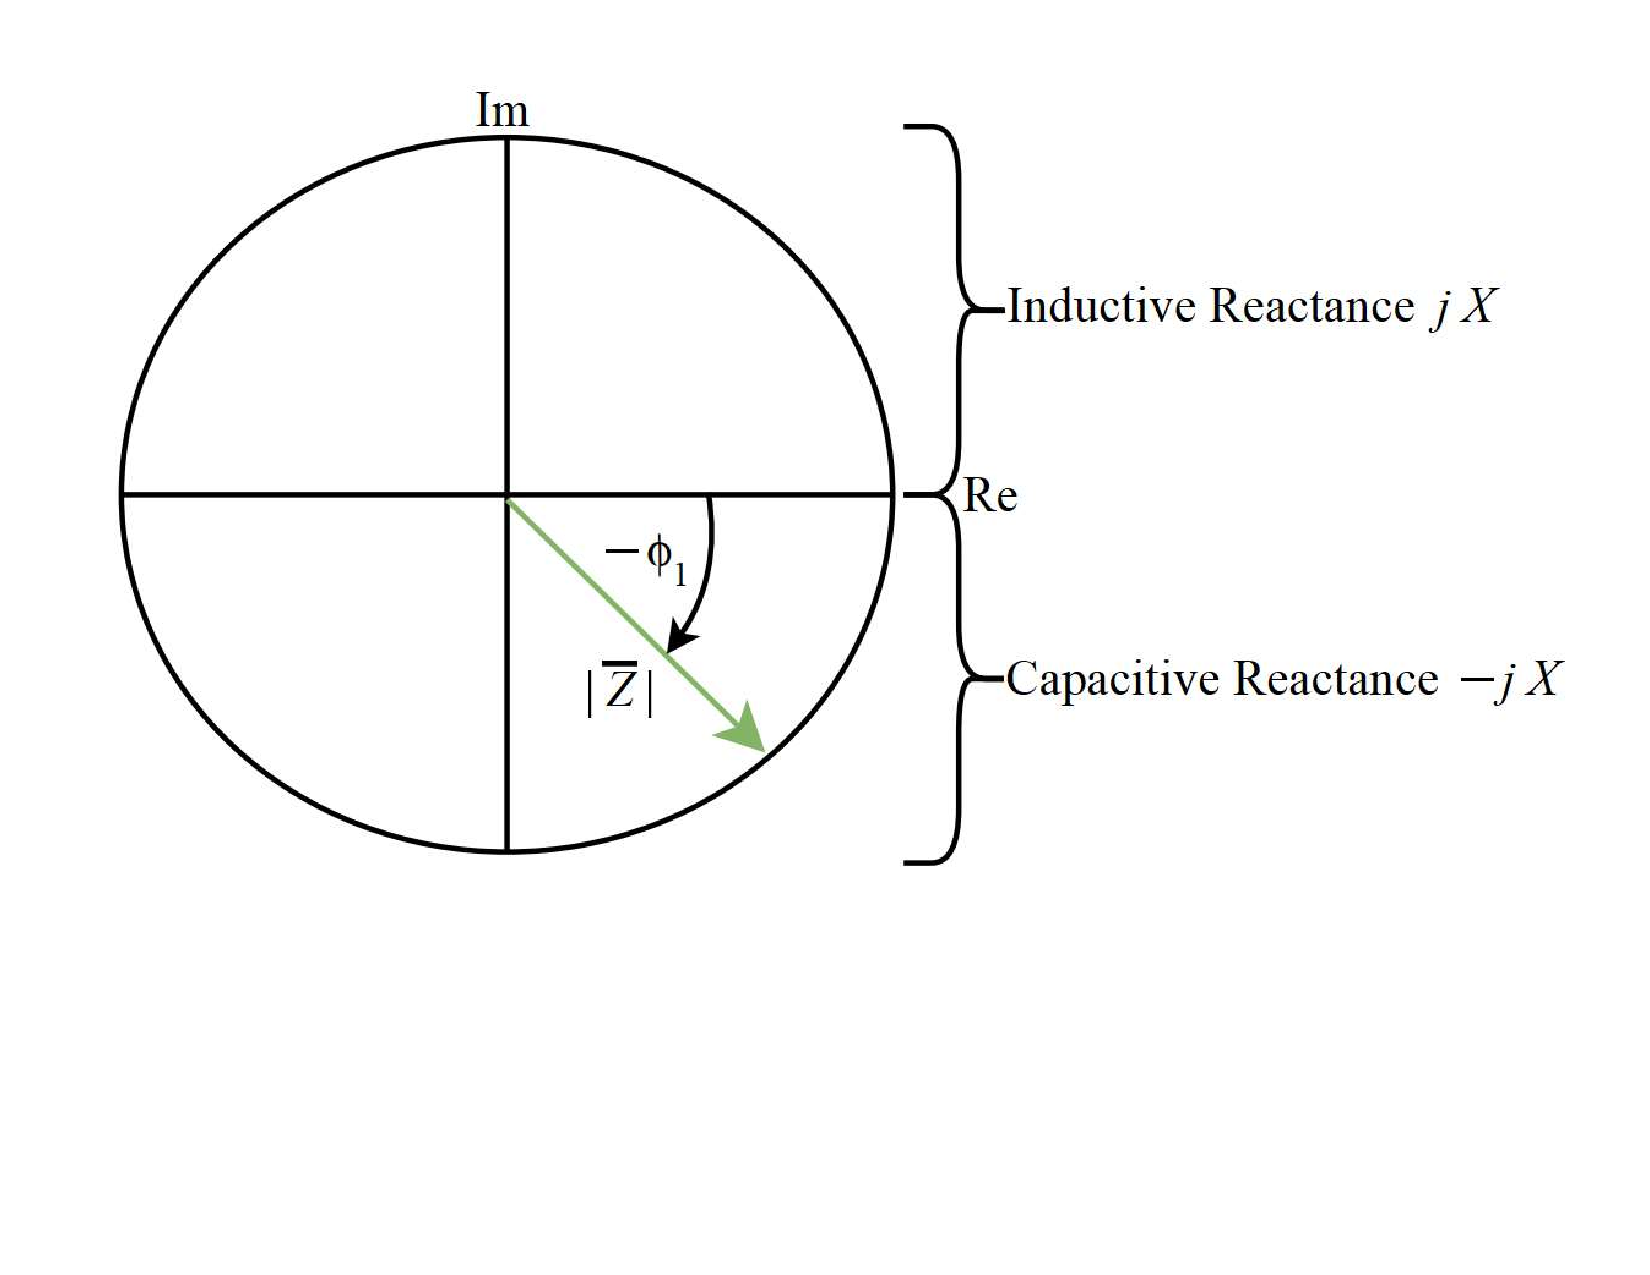
\includegraphics[clip, trim=0 175 0 0, width=0.60\textwidth]{Sections/4_TechnicalAnalysis/Figures/4_1_CapImpedance.pdf}
    \caption{The impedance vector of a capacitive DUT will be located in the 4th quadrant as shown by the $\bar Z$ vector. An impedance pointing into the 4th quadrant is denoted a \textit{capacitive reactance} while an impedance in the 1st quadrant is called a \textit{inductive reactance}.}
    \label{fig:4_1_CapImpedance}
\end{figure}

As shown by figure \ref{fig:4_1_CapImpedance} the sign of the imaginary part of the complex impedance $Z = R \pm jX$ will be an important part to track in order to identify the type of DUT. A similar analysis can be performed with an inductive DUT, in this case the current will lag the voltage as shown on the phasor diagram on figure \ref{fig:4_1_IndPhasor}.
\begin{figure}[H]
    \centering
    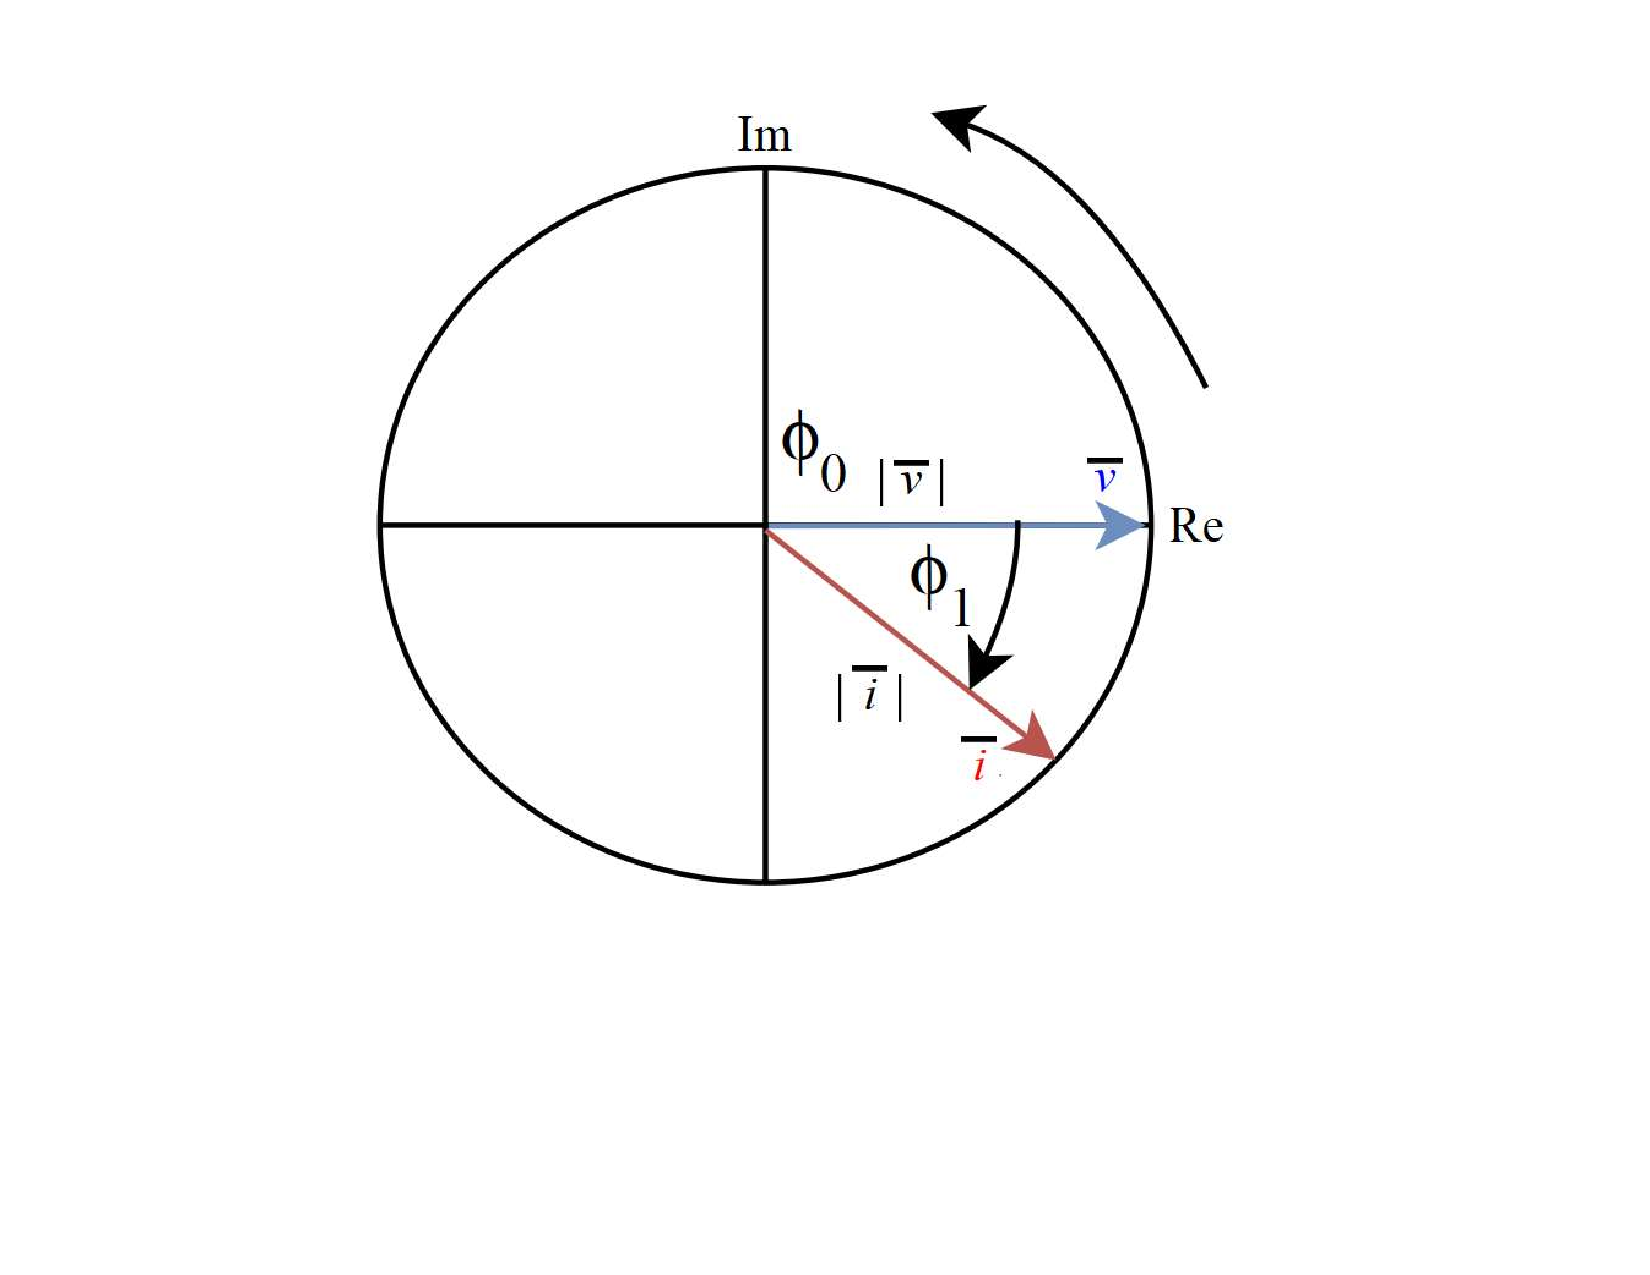
\includegraphics[clip, trim=0 175 0 0, width=0.75\textwidth]{Sections/4_TechnicalAnalysis/Figures/4_1_InductivePhasor.pdf}
    \caption{For an inductive DUT the voltage waveform will lead the current waveform. Note how the phase angle $\phi_1$ of $\bar i$ is going against the established positive direction of the coordinate system.}
    \label{fig:4_1_IndPhasor}
\end{figure}

The current phasor $\bar i$ is lagging the voltage phasor $\bar v$ by a negative phase angle relative to the positive direction of the phasor diagram and will have the phase angle shown in eq \ref{eq:4_1_IndPhase}.

\begin{equation}\label{eq:4_1_IndPhase}
    \Delta \phi = \phi_0 -(-\phi_1) =\phi_1 \bigg\rvert_{\phi_0 = 0}
\end{equation}

Applying eq \ref{eq:4_1_IndPhase} to eq \ref{eq:4_1_Impedance} gives the impedance of an inductive DUT as shown in 
\begin{equation}\label{eq:4_1_IndImpedance2}
    \bar Z_l = \frac{|\bar v|}{|\bar i| [cos(\phi_1) -j\cdot sin(\phi_1)]}
\end{equation}
Once again Eulers formula is applied like in eq \ref{eq:4_1_CapImpedance4} on eq \ref{eq:4_1_IndImpedance2} and gives eq \ref{eq:4_1_IndImpedance3}

\begin{equation}\label{eq:4_1_IndImpedance3} 
    \bar Z_l = \frac{|\bar v|}{|\bar i|} \cdot \frac{1}{cos(\phi_1) - j\cdot sin(\phi_1)} = |\bar Z| \cdot \mathrm (e^{-j\phi})^{-1}
\end{equation}
Eq \ref{eq:4_1_IndImpedance3} is simplified to equation \ref{eq:4_1_IndImpedance4}.
\begin{equation}\label{eq:4_1_IndImpedance4} 
    \bar Z_l =|\bar Z| \cdot \mathrm e^{j\phi}
\end{equation}
Equation \ref{eq:4_1_IndImpedance4} has positive phase and is an impedance vector now pointing into the first quadrant which signifies that it has inductive reactance as shown on figure \ref{fig:4_1_IndImpedance} and figure \ref{fig:4_1_CapImpedance}.

\begin{figure}[H]
    \centering
    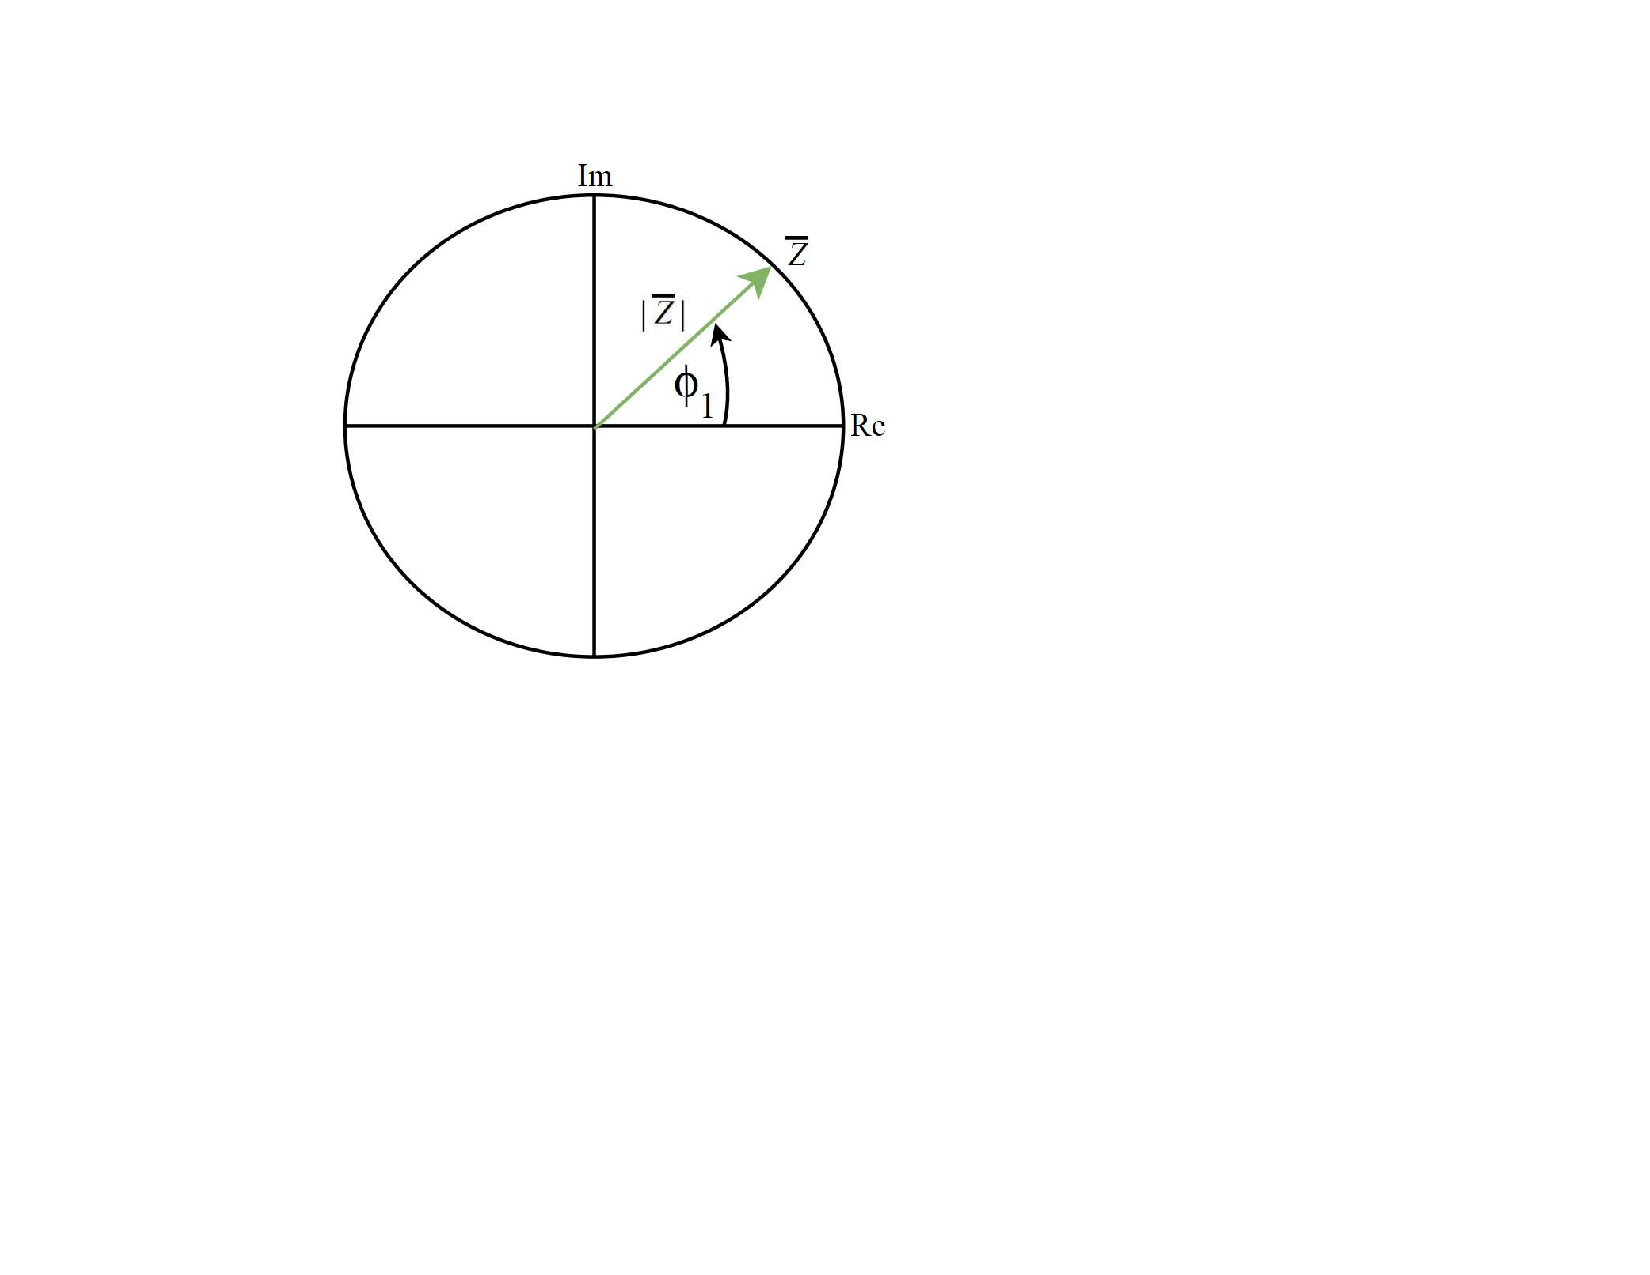
\includegraphics[clip, trim=0 275 0 0, width=1\textwidth]{Sections/4_TechnicalAnalysis/Figures/4_1_IndImpedance.pdf}
    \caption{The impedance an of inductive DUT is pointing into the first quadrant which means the impedance has inductive reactance.}
    \label{fig:4_1_IndImpedance}
\end{figure}

For the case where the DUT has no reactive components the reference voltage waveform will be \textit{in phase} with the resulting current waveform as shown on figure \ref{fig:4_1_ResImpedance}.

\begin{figure}[H]
    \centering
    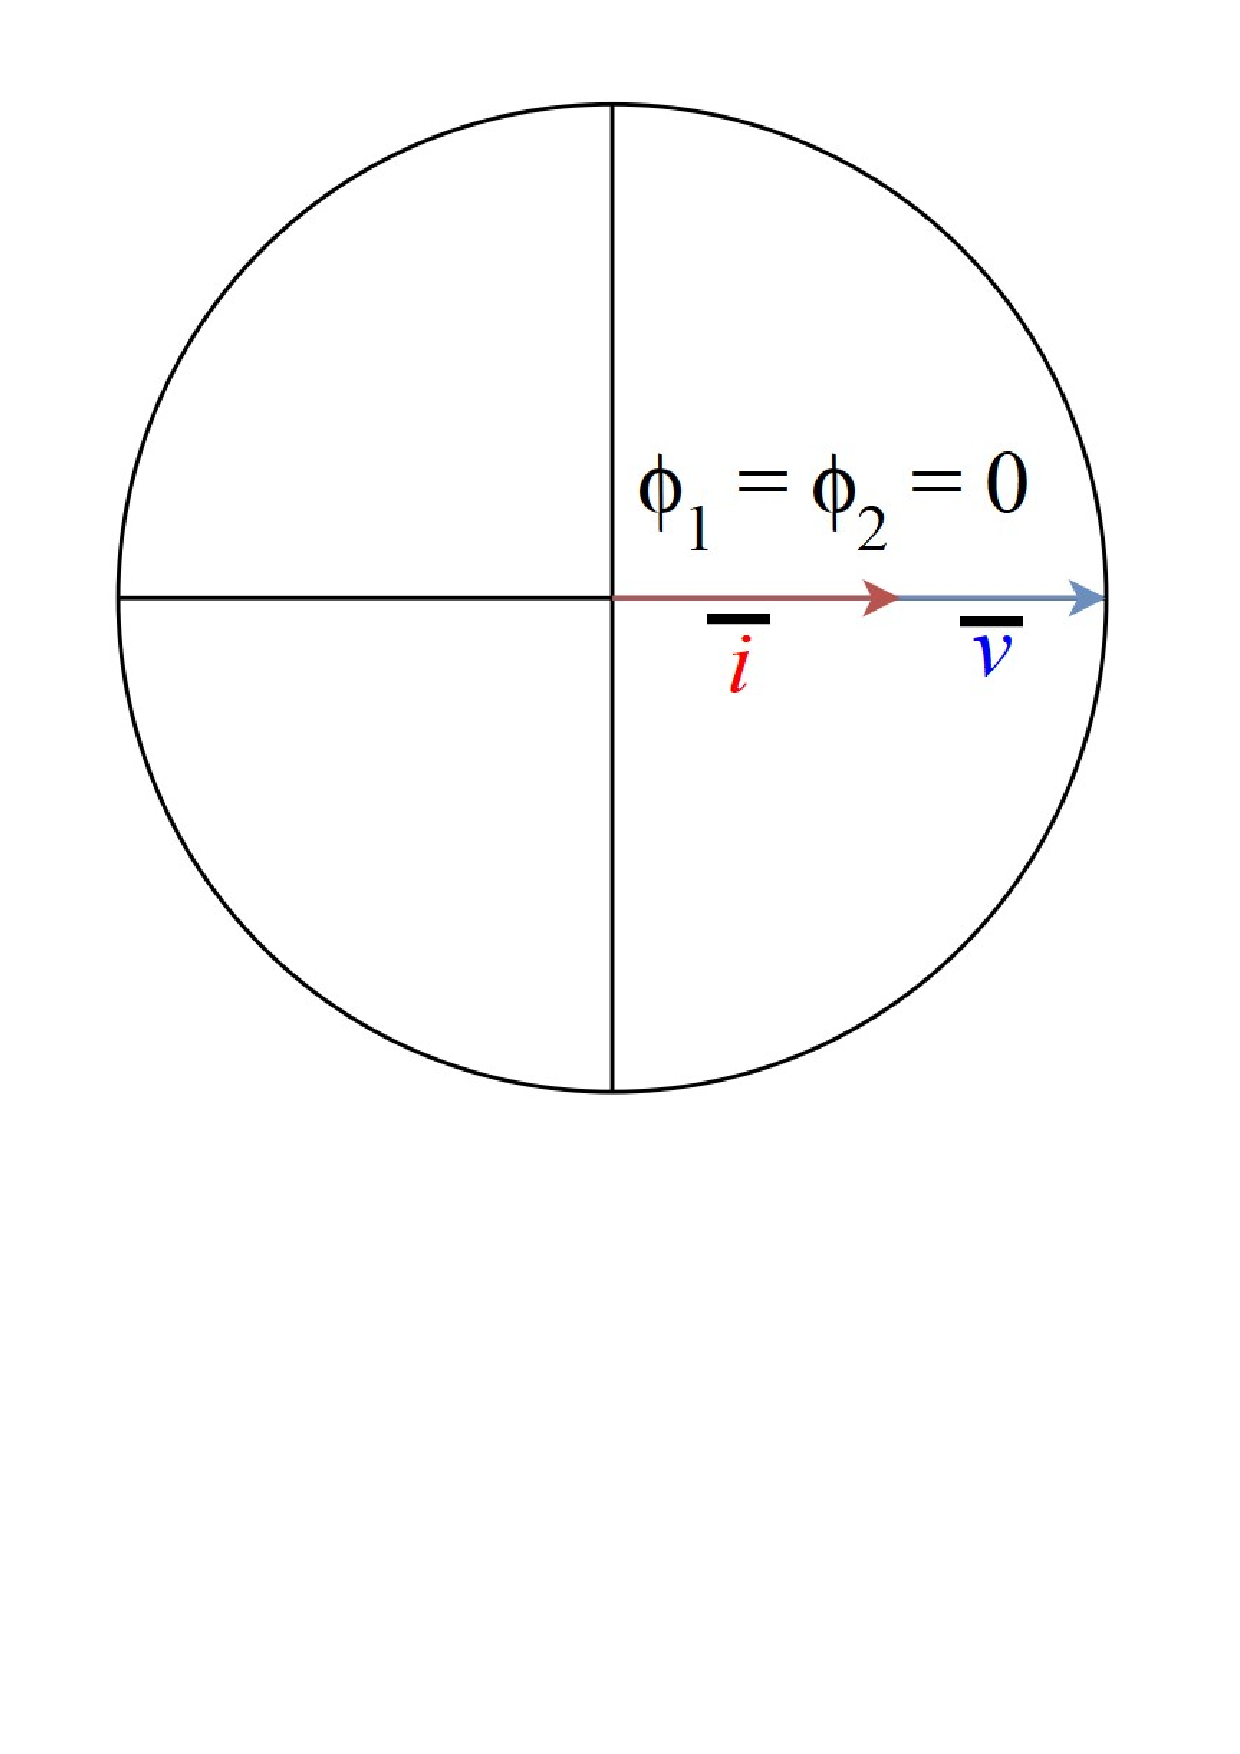
\includegraphics[clip, trim=0 275 0 0, width=0.4\textwidth]{Sections/4_TechnicalAnalysis/Figures/4_1_ResPhasor.pdf}
    \caption{The current vector is in phase with the reference voltage vector. Both vectors lie on the real axis and the impedance will be purely resistive as a result.}
    \label{fig:4_1_ResImpedance}
\end{figure}

The phasor diagram on \ref{fig:4_1_ResImpedance} has the current vector $\bar i$ and the voltage vector $\bar v$ in phase $\phi = 0$ and 
the resulting impedance will be as eq \ref{eq:4_1_Resistance}.
\begin{equation}\label{eq:4_1_Resistance}
    \bar Z_c = \frac{|\bar v| [cos(0) +j\cdot sin(0)]}{|\bar i| [cos(0) +j\cdot sin(0)]}
\end{equation}

With $cos(0) = 1$ and  $sin(0) = 1$ the impedance $\bar Z$ in eq \ref{eq:4_1_Resistance} is purely resistive. It has no imaginary component and thus has no phase shift and depends only on the magnitude of $\bar i$ and $\bar v$ as shown in eq \ref{eq:4_2_Resistance}
\begin{equation}\label{eq:4_2_Resistance}
    \bar Z_c = \frac{|\bar v|}{|\bar i|}
\end{equation}

Equations \ref{eq:4_1_CapImpedance4}, \ref{eq:4_1_IndImpedance4} and \ref{eq:4_2_Resistance} show that, in order to calculate the impedance of a DUT, an impedance analyzer must be able to measure the magnitude and phase of the reference voltage waveform $\bar v_{ref}$ along with the magnitude and phase of the resulting current waveform $\bar i_{dut}$. The system may already have some information on $\bar v_{ref}$ but in either case it must be known. It is possible to calculate the value of $L, C, R, D, Q..$ and so on once the impedance is known as will be shown in the next chapter.
\subsection{Derived quantities} \label{subsec:DerivedQuantities}
The value of inductance, capacitance or resistance can be calculated once the impedance of the DUT is known, along with the dissipation and quality factor. This chapter will show how this can be achieved. Consider that in section \ref{sec:ImpedanceAnalysis} where the impedance of a DUT could be written in the rectangular form $Z = R \pm jX$. The $jX$ term represents the capacitive, or inductive, reactance that could be used to find the inductance or capacitance value of the DUT.

To find $jX$ is trivial and will be done only for a capacitor, the process for an inductor is the same. Consider the circuit on figure \refq{fig:4_1_1_CapCircuit} with a voltage source, $v(t)$, connected across a capacitor and a current $i(t)$ flowing in the circuit. 
\begin{figure}[H]
    \centering
    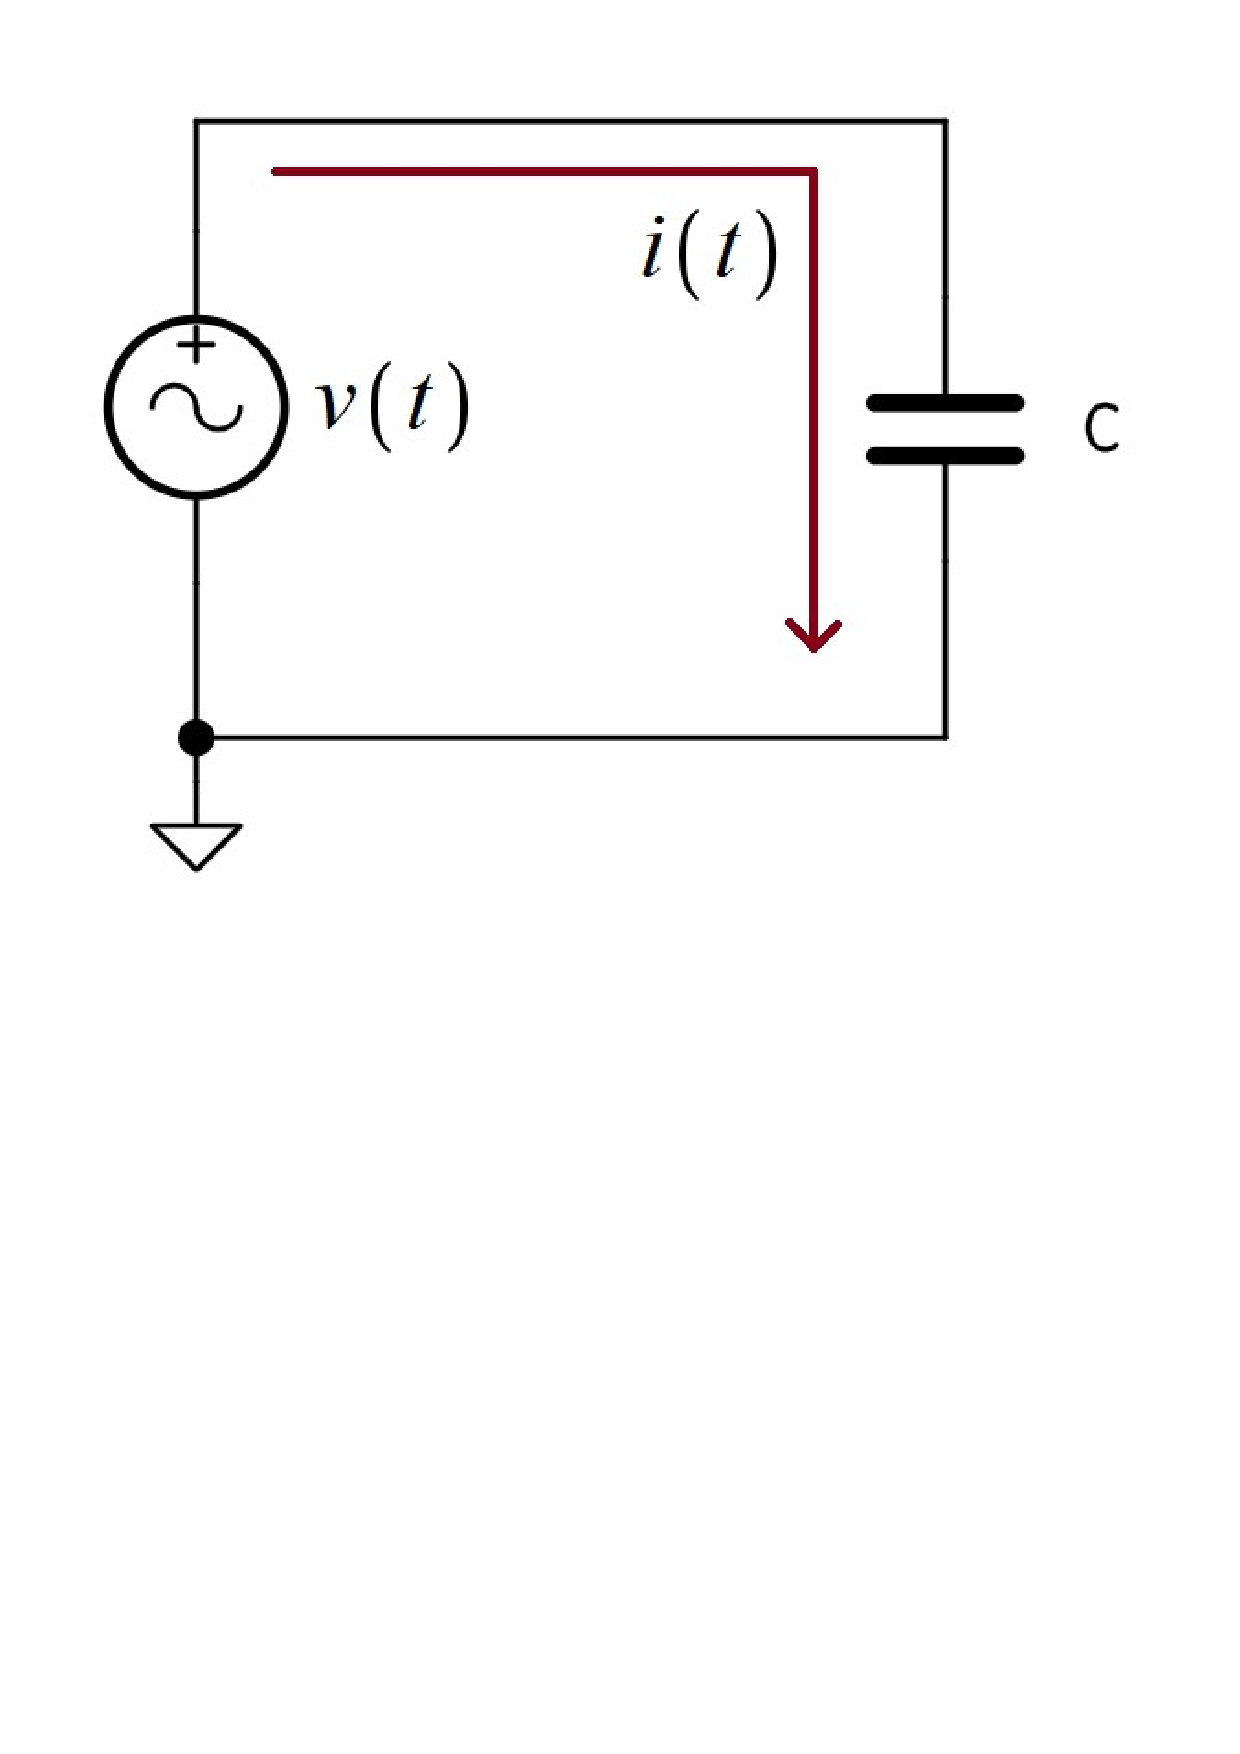
\includegraphics[clip, trim=0 400 0 0, width=0.60\textwidth]{Sections/4_TechnicalAnalysis/Figures/4_1_1_CapCircuit.pdf}
    \caption{An AC voltage source, $v(t)$, across a capacitor causes a current, $i(t)$, to flow through it.}
    \label{fig:4_1_1_CapCircuit}
\end{figure}

The current in the circuit is, because of the capacitor, as in eq \refq{eq:4_1_1_CapCurrent}.
\begin{equation}\label{eq:4_1_1_CapCurrent}
    i(t) = C\cdot\frac{d}{dt} (v(t))
\end{equation}
Transforming \refq{eq:4_1_1_CapCurrent} into the frequency domain with the laplace transform gives eq \refq{eq:4_1_1_CapCurrent2}.
\begin{equation}\label{eq:4_1_1_CapCurrent2}
    \Laplace\{\/i(t)\}\ = \Laplace\{\/C\cdot\frac{d}{dt} (v(t))\} \rightarrow I(s) = C\cdot(sV(s) - v(t=0^-))
\end{equation}
The circuit is supplied by an AC source and it is assumed that the circuit has reached a steady-state so that the initial condition of the voltage source is $v(t=0^-) = 0$. Solving for the reactance of the circuit $V(s) / I(s)$ gives eq \refq{eq:4_1_1_CapCurrent3}.
\begin{equation}\label{eq:4_1_1_CapCurrent3}
    \frac{V(s)}{I(s)} =X_c(s)= \frac{1}{sC}
\end{equation}
Substituting the laplace variable $s$ with $s = 0 + j\omega$ gives eq \refq{eq:4_1_1_CapCurrent4}.
\begin{equation}\label{eq:4_1_1_CapCurrent4}
    X_c(\omega) = \frac{1}{j\omega C}=-\frac{j}{\omega C}
\end{equation}
Note that the complex laplace variable is defined as $s = \sigma + j\omega$. The real part $\sigma$ represents exponential growth. By assuming the circuit is in steady-state, there is no exponential growth so $\sigma = 0$. The impedance for a circuit dominated by a capacitance will have the form $Z = R -\frac{j}{\omega C}$ as shown in eq \refq{eq:4_1_1_CapCurrent4}.

A similar exercise can be performed if the capacitor on figure \refq{fig:4_1_1_CapCircuit} was swapped with an inductor. The results is the expression for inductive reactance in eq \refq{eq:4_1_1_IndReactance}.
\begin{equation}\label{eq:4_1_1_IndReactance}
    X_l(\omega) = j \omega L
\end{equation}
Note how the negative sign of the capacitive reactance and the positive sign of the inductive reactance matches the results found in section \refq{sec:ImpedanceAnalysis}.

Real capacitors and inductors have undesired parasitic parameters like 

\subsection{Reactance} \label{subsec:Reactance}
To find $jX$ is trivial and will be done only for a capacitor, the process for an inductor is the same. Consider the circuit on figure \refq{fig:4_1_1_CapCircuit} with a voltage source, $v(t)$, connected across a capacitor and a current $i(t)$ flowing in the circuit. 
\begin{figure}[H]
    \centering
    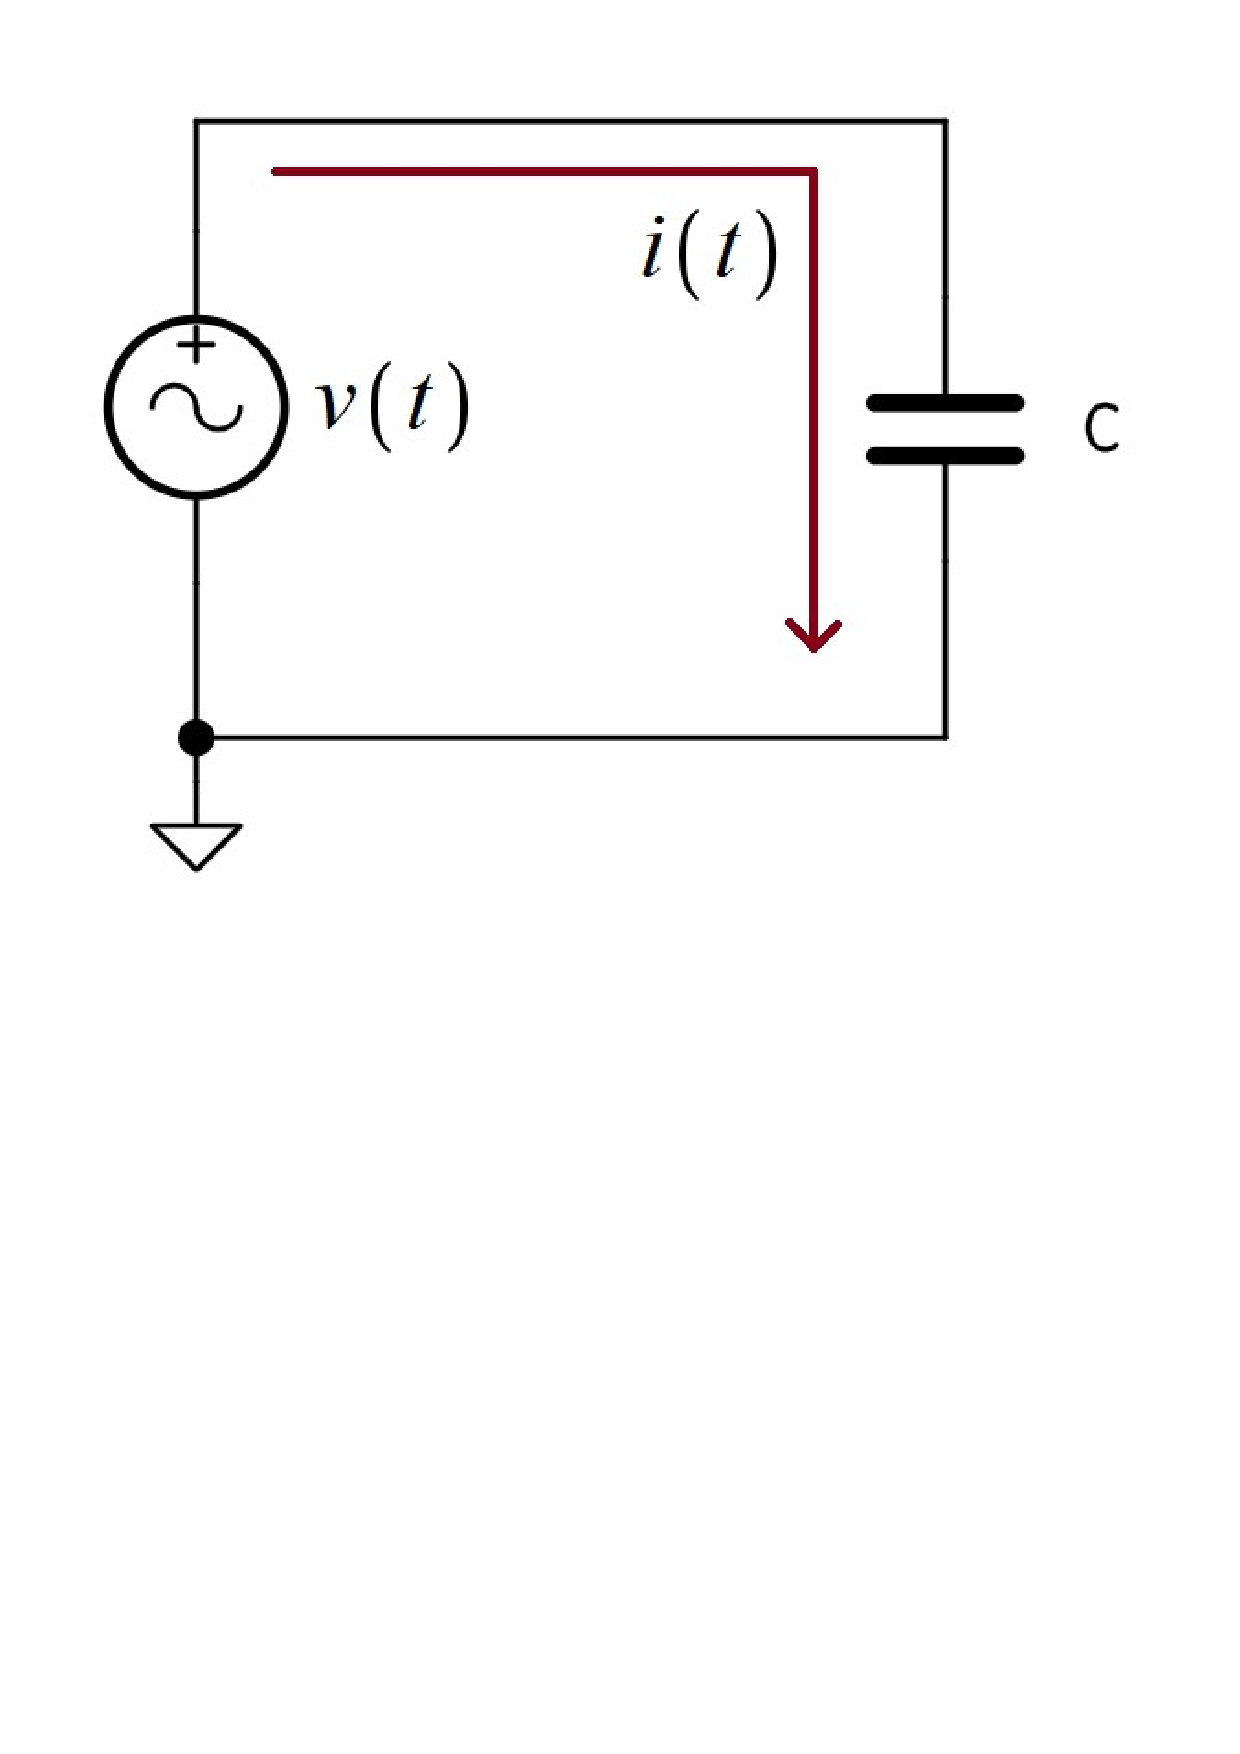
\includegraphics[clip, trim=0 400 0 0, width=0.60\textwidth]{Sections/4_TechnicalAnalysis/Figures/4_1_1_CapCircuit.pdf}
    \caption{An AC voltage source, $v(t)$, across a capacitor causes a current, $i(t)$, to flow through it.}
    \label{fig:4_1_1_CapCircuit}
\end{figure}

The current in the circuit is, because of the capacitor, as in eq \refq{eq:4_1_1_CapCurrent}.
\begin{equation}\label{eq:4_1_1_CapCurrent}
    i(t) = C\cdot\frac{d}{dt} (v(t))
\end{equation}
Transforming \refq{eq:4_1_1_CapCurrent} into the frequency domain with the laplace transform gives eq \refq{eq:4_1_1_CapCurrent2}.
\begin{equation}\label{eq:4_1_1_CapCurrent2}
    \Laplace\{\/i(t)\}\ = \Laplace\{\/C\cdot\frac{d}{dt} (v(t))\} \rightarrow I(s) = C\cdot(sV(s) - v(t=0^-))
\end{equation}
The circuit is supplied by an AC source and it is assumed that the circuit has reached a steady-state so that the initial condition of the voltage source is $v(t=0^-) = 0$. Solving for the reactance of the circuit $V(s) / I(s)$ gives eq \refq{eq:4_1_1_CapCurrent3}.
\begin{equation}\label{eq:4_1_1_CapCurrent3}
    \frac{V(s)}{I(s)} =X_c(s)= \frac{1}{sC}
\end{equation}
Substituting the laplace variable $s$ with $s = 0 + j\omega$ gives eq \refq{eq:4_1_1_CapCurrent4}.
\begin{equation}\label{eq:4_1_1_CapCurrent4}
    X_c(\omega) = \frac{1}{j\omega C}=-\frac{j}{\omega C}
\end{equation}
Note that the complex laplace variable is defined as $s = \sigma + j\omega$. The real part $\sigma$ represents exponential growth. By assuming the circuit is in steady-state, there is no exponential growth so $\sigma = 0$. The impedance for a circuit dominated by a capacitance will have the form $Z = R -\frac{j}{\omega C}$ as shown in eq \refq{eq:4_1_1_CapCurrent4}.

The value of capacitance can be found with eq \refq{eq:4_1_1_CapCurrent4} by just solving for C. This gives the phasor in eq \ref{eq:4_1_1_CapCurrent5}
\begin{equation}\label{eq:4_1_1_CapCurrent5}
    C(\omega)=-\frac{j}{X_C\cdot \omega}
\end{equation}
The quantity of interest at this point is the magnitude of capacitance as shown in eq \refq{eq:4_1_1_CapCurrent6}.
\begin{equation}\label{eq:4_1_1_CapCurrent6}
    |C(\omega)|= \sqrt{\left(-\frac{1}{X_C\cdot \omega}\right)^2} =\frac{1}{X_c\cdot \omega} 
\end{equation}

The result in eq \refq{eq:4_1_1_CapCurrent5} is obvious as the phasor in eq \refq{eq:4_1_1_CapCurrent5} is just pointing down the imaginary axis in the complex plane and thus has a magnitude of $abs(C)$. A similar exercise can be performed if the capacitor on figure \refq{fig:4_1_1_CapCircuit} was swapped with an inductor. The results is the expression for inductive reactance in eq \refq{eq:4_1_1_IndReactance}.
\begin{equation}\label{eq:4_1_1_IndReactance}
    X_l(\omega) = j \omega L
\end{equation}

Much like eq \refq{eq:4_1_1_CapCurrent6} the inductance value can be found with eq \refq{eq:4_1_1_IndReactance}. This is done in eq \refq{eq:4_1_1_IndReactance2}.

\begin{equation}\label{eq:4_1_1_IndReactance2}
    L(\omega) = \frac{X_l(\omega)}{j\omega} = -j\frac{X_l(\omega)}{\omega}
\end{equation}

Similar to eq \refq{eq:4_1_1_CapCurrent6} the magnitude of inductance is found and is as shown in eq \refq{eq:4_1_1_IndReactance3}.

\begin{equation}\label{eq:4_1_1_IndReactance3}
    |L(\omega)| = \sqrt{\left(-\frac{X_l(\omega)}{\omega}\right)^2} = \frac{X_l(\omega)}{\omega}
\end{equation}
\subsection{Reactive Power} \label{subsec:ReactivePower}
If a voltage $v$ in $\phi = 0$ is applied across a pure reactance, as in eq \refq{eq:4_1_1_CapCurrent4}, it will cause the resulting current to be phase shifted by \SIQ{90}{\degree}. This is shown in eq \ref{eq:4_1_1_ReactiveCurrentPhaseShift}. 
\begin{equation}\label{eq:4_1_1_ReactiveCurrentPhaseShift}
    i(\omega) = \frac{v(\omega)}{-\frac{j}{\omega C}} = v(\omega) \cdot j \omega C 
\end{equation}
The current is leading the voltage as shown in \ref{eq:4_1_1_ReactiveCurrentPhaseShift} and figure \ref{fig:4_1_1_ReactanceCurrentLeadVoltage}.
\begin{figure}[H]
    \centering
    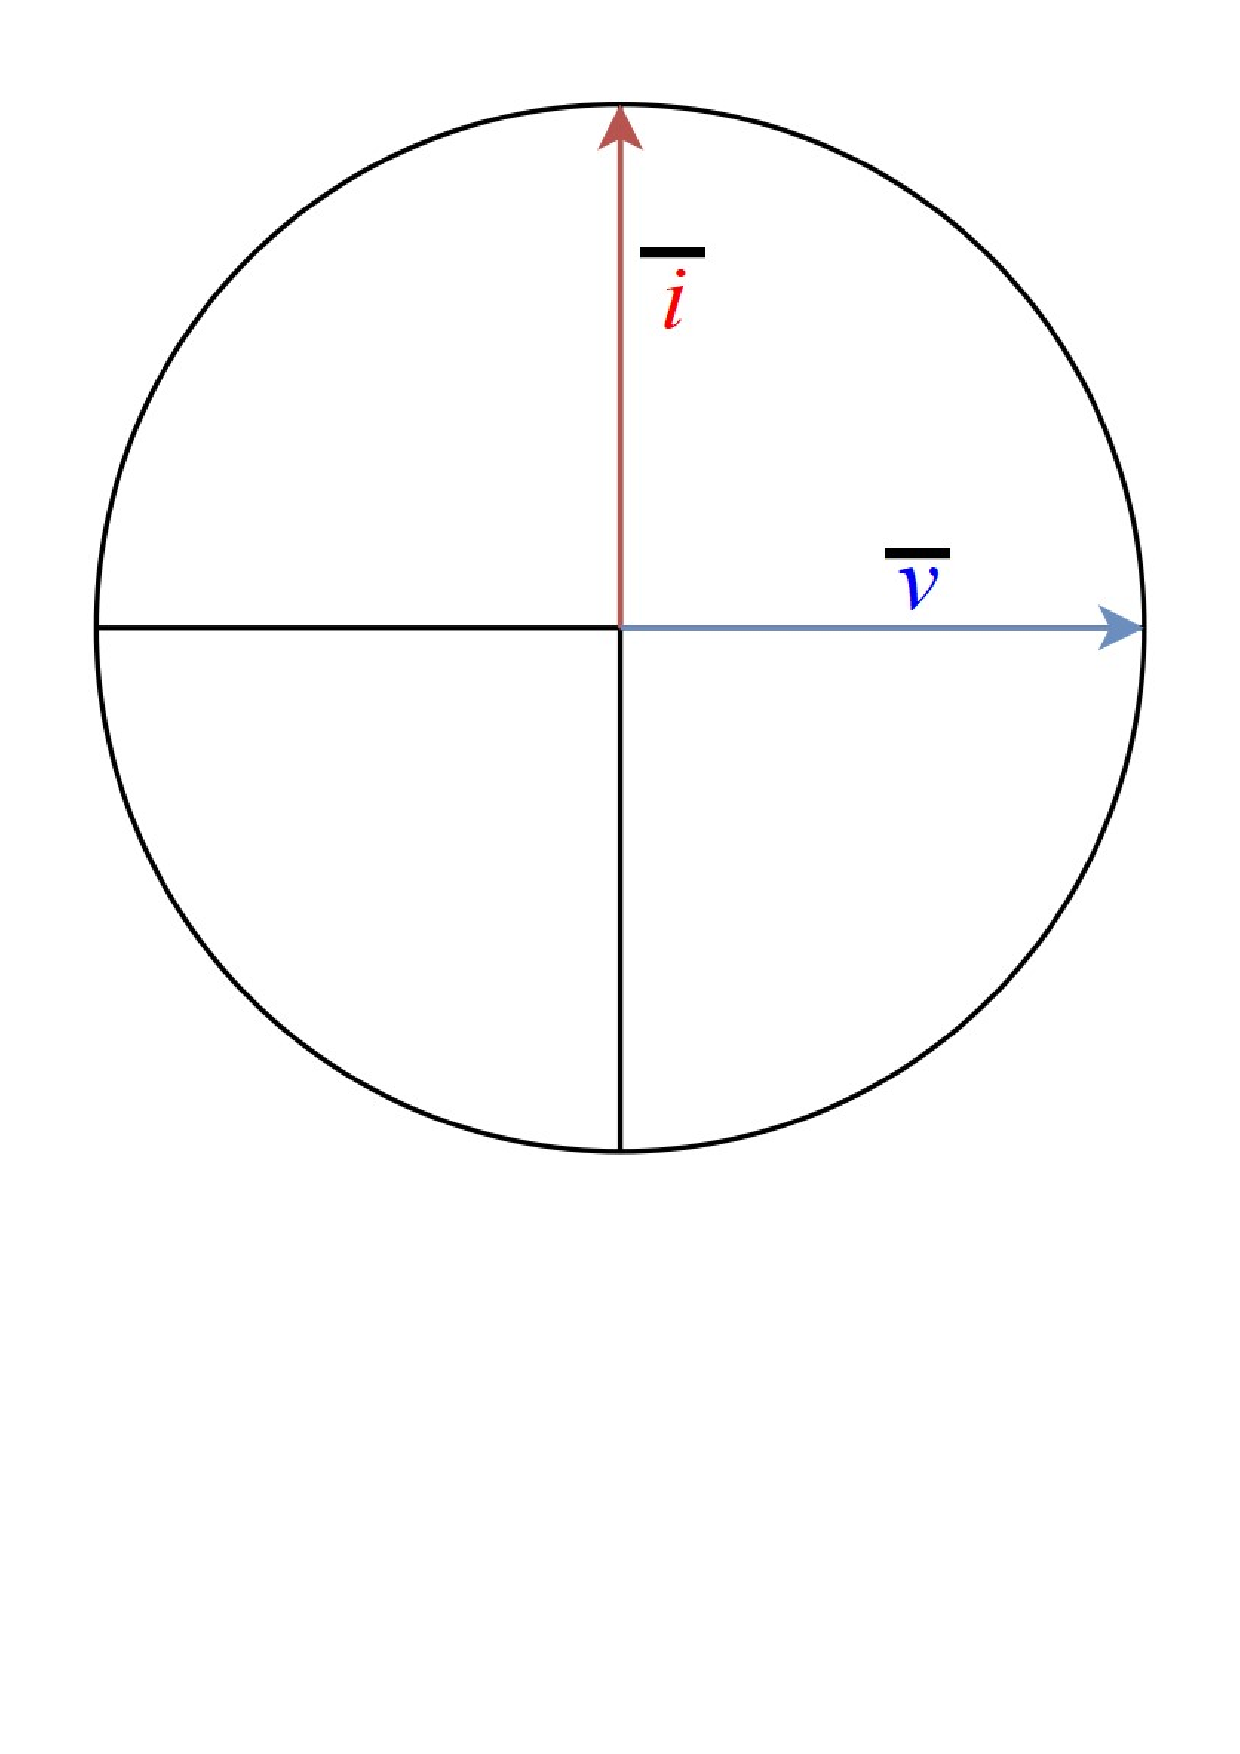
\includegraphics[clip, trim=0 250 0 0, width=0.4\textwidth]{Sections/4_TechnicalAnalysis/Figures/4_1_1_ReactanceCurrentPhase.pdf}
    \caption{The current is leading the voltage by \SIQ{90}{\degree} when a voltage is applied across the capacitive reactance.}
    \label{fig:4_1_1_ReactanceCurrentLeadVoltage}
\end{figure}

The power dissipated in the reactance is the vector product of the current and voltage as shown in equation \refq{eq:4_1_1_ReactivePowerLossLess}.
\begin{equation}\label{eq:4_1_1_ReactivePowerLossLess}
    P = \bar i \cdot \bar v = |\bar i| |\bar v| cos(\phi)
\end{equation}

Since $\phi = \frac{\pi}{2}$ (or \SIQ{90}{\degree}) then $cos(\pi/2) = 0$ and the power dissipated in the reactance is 0 as shown in eq \ref{eq:4_1_1_ReactivePowerLossLess2}
\begin{equation}\label{eq:4_1_1_ReactivePowerLossLess2}
    P = \bar i \cdot \bar v = |\bar i| |\bar v| cos\left(\frac{\pi}{2}\right) = 0
\end{equation}
This result means that an ideal capacitor with an impedance that is a pure reactance cannot dissipate any power. It is lossless. The same is true for inductors with the current vector lagging the voltage by \SIQ{90}{\degree}. Real components are not purely reactive however, they have resistance in the leads and materials used to construct them and the dieelectric material in a capacitor can absorb energy leading to losses. 

\subsection{Loss Tangent, ESR and Quality} \label{subsec:LossTangent}

Real components are not purely reactive and will have resistance in them, so their impedance vector will not be pointing straight up or down the imaginary axis as shown on figure \refq{fig:4_1_1_LossTangent1} and in section \refq{sec:ImpedanceAnalysis}.

\begin{figure}[H]
    \centering
    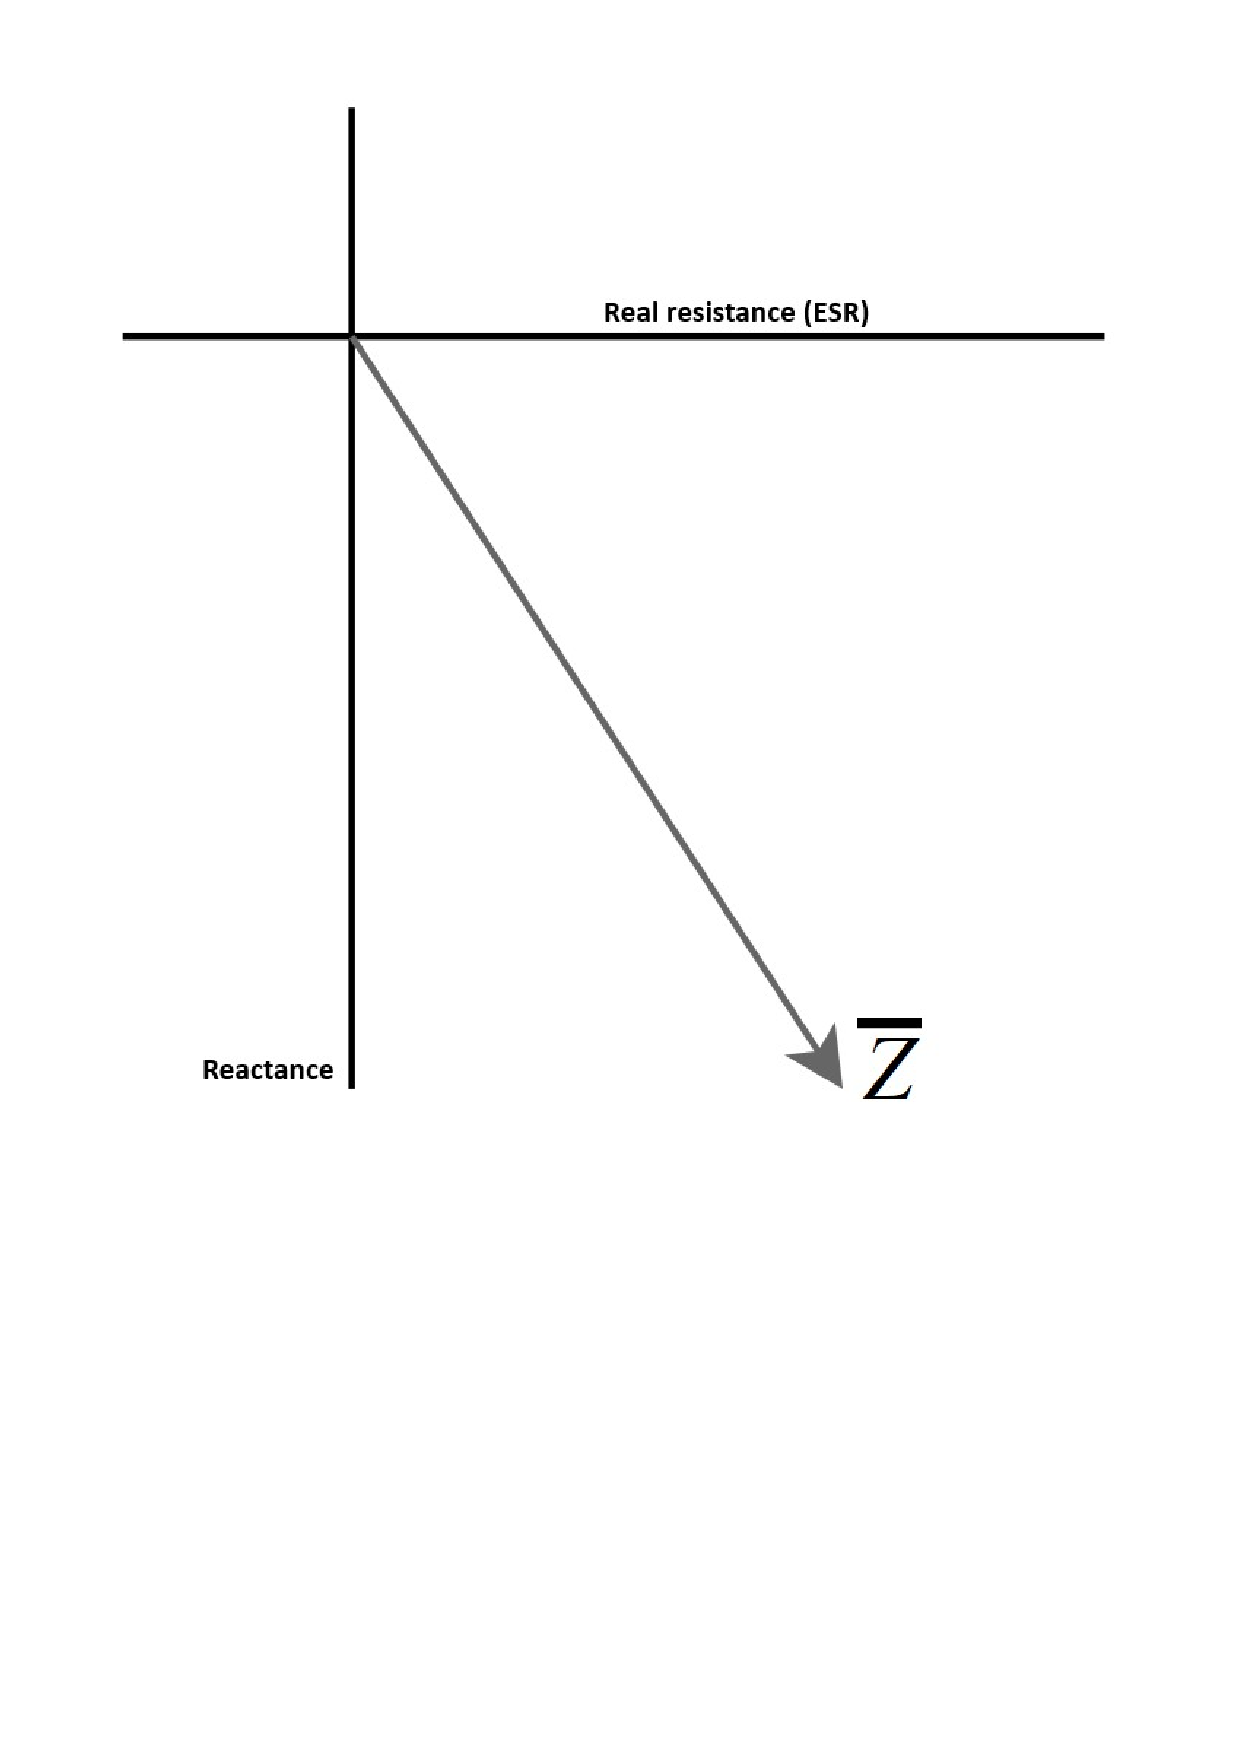
\includegraphics[clip, trim=0 250 0 0, width=0.4\textwidth]{Sections/4_TechnicalAnalysis/Figures/4_1_4_LossTangent1.pdf}
    \caption{The capacitor is not ideal. It has a finite amount of resistance in the materials it is made of.}
    \label{fig:4_1_1_LossTangent1}
\end{figure}

The impedance $|\bar Z|$ is a vector sum of the components real resistance (ESR) and the components reactance. A \textit{large} ESR (equivalent series resistance) will cause the impedance to deviate from the ideal pure reactance of the component and the losses in the device will increase as power can be dissipated in real resistances.

The angle between the impedance and the ideal reactance axis is called the \textit{loss angle} and is sometimes stated in component datasheets. It relates the resistance of a device to it's reactance. A large angle means the capacitor has large resistance and vice versa. This angle is shown on figure \refq{fig:4_1_1_LossTangent2} and is denoted $\delta$.

\begin{figure}[H]
    \centering
    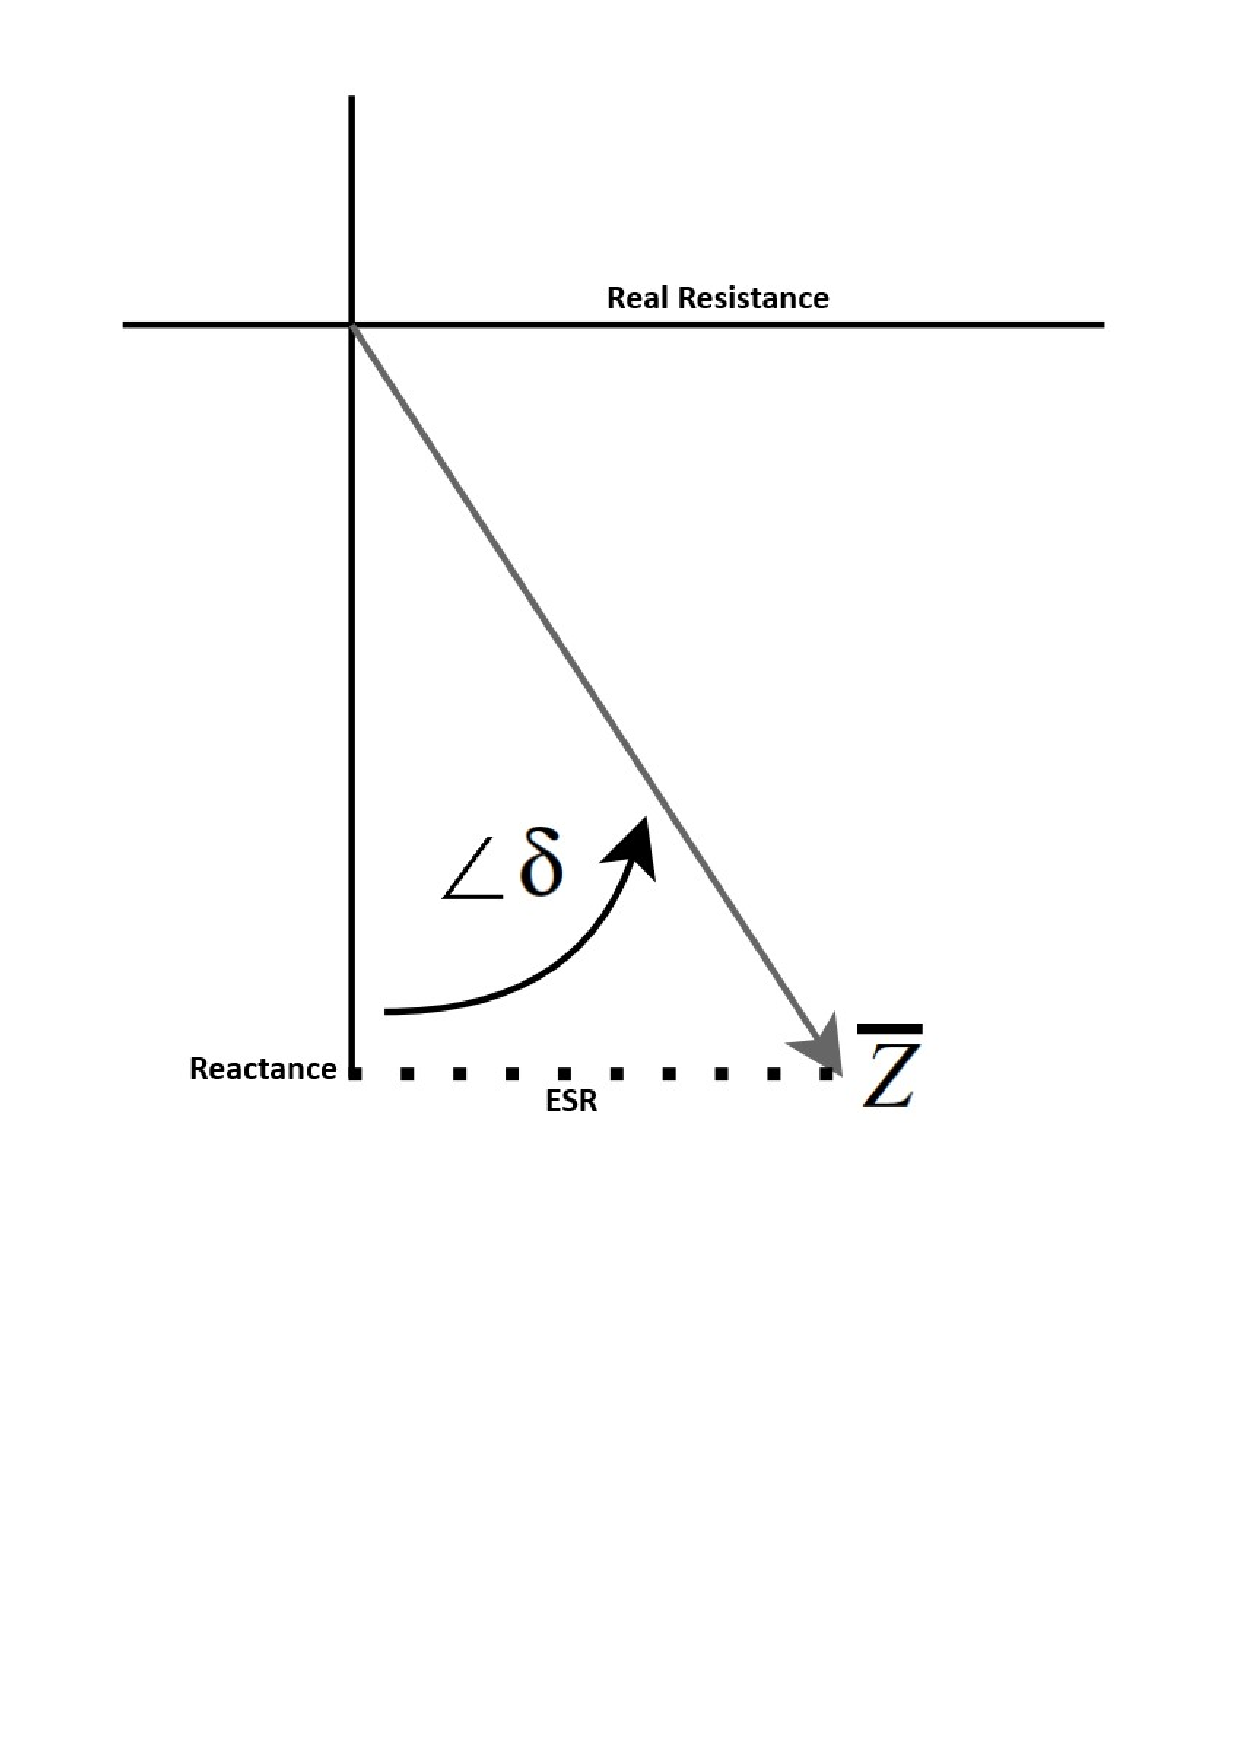
\includegraphics[clip, trim=0 275 0 0, width=0.4\textwidth]{Sections/4_TechnicalAnalysis/Figures/4_1_4_LossTangent2.pdf}
    \caption{The loss angle is the angle from origin between $\bar Z$ and the imaginary axis.}
    \label{fig:4_1_1_LossTangent2}
\end{figure}

The loss angle on figure \refq{fig:4_1_1_LossTangent2} can be found in a number of ways, but it is often done with the tangent relation as shown in equation \refq{eq:4_1_1_LossAngle}. For this reason it is also called the \textit{loss tangent}.
\begin{equation}\label{eq:4_1_1_LossAngle}
    tan(\delta) =\frac{ESR}{|X|} 
\end{equation}
Where $X$ is the capacitive reactance in this case. The value $tan(\delta)$ is also called the \textit{dissipation factor} and $DF = tan(\delta)$. Electrolytic capacitors have relatively high ESR and will have a higher dissipation factor, so they will dissipate more power than a ceramic capacitor with a low dissipation factor would. The ESR can be found if the dissipation factor is known as shown in eq \refq{eq:4_1_1_ESR}.
\begin{equation}\label{eq:4_1_1_ESR}
    ESR =  tan(\delta)\cdot |X|
\end{equation}
An instrument measuring an impedance will, however, already know the ESR as the real part of the impedance.

Another common quantity that is also related to the loss tangent is the \textit{quality factor} which is simply the reciprocal of the dissipation factor as shown in eq \refq{eq:4_1_1_Q}.
\begin{equation}\label{eq:4_1_1_Q}
    Q = \frac{1}{DF} = \frac{|X|}{ESR}
\end{equation}
The quality factor will be high if ESR is low and vice versa.




\subsection{Series to Parallel Conversion} \label{subsec:SeriesToParallel}
The $\bar v$ and $\bar i$ signals described in section \refq{sec:ImpedanceAnalysis} can be used to characterize the DUT, but the signals say nothing about how the impedance is supposed to be modelled. The impedance of a DUT could have the form shown on figure \refq{fig:4_1_5_DUTXSeriesParallel} where the DUT has a series resistance $R_s$ in series with a parallel connection of a pure reactance $X$, from either a capacitor or inductor, and a parallel resistor $R_p$. Both $R_s$ and $R_p$ cause power dissipation in the DUT.

\begin{figure}[H]
    \centering
    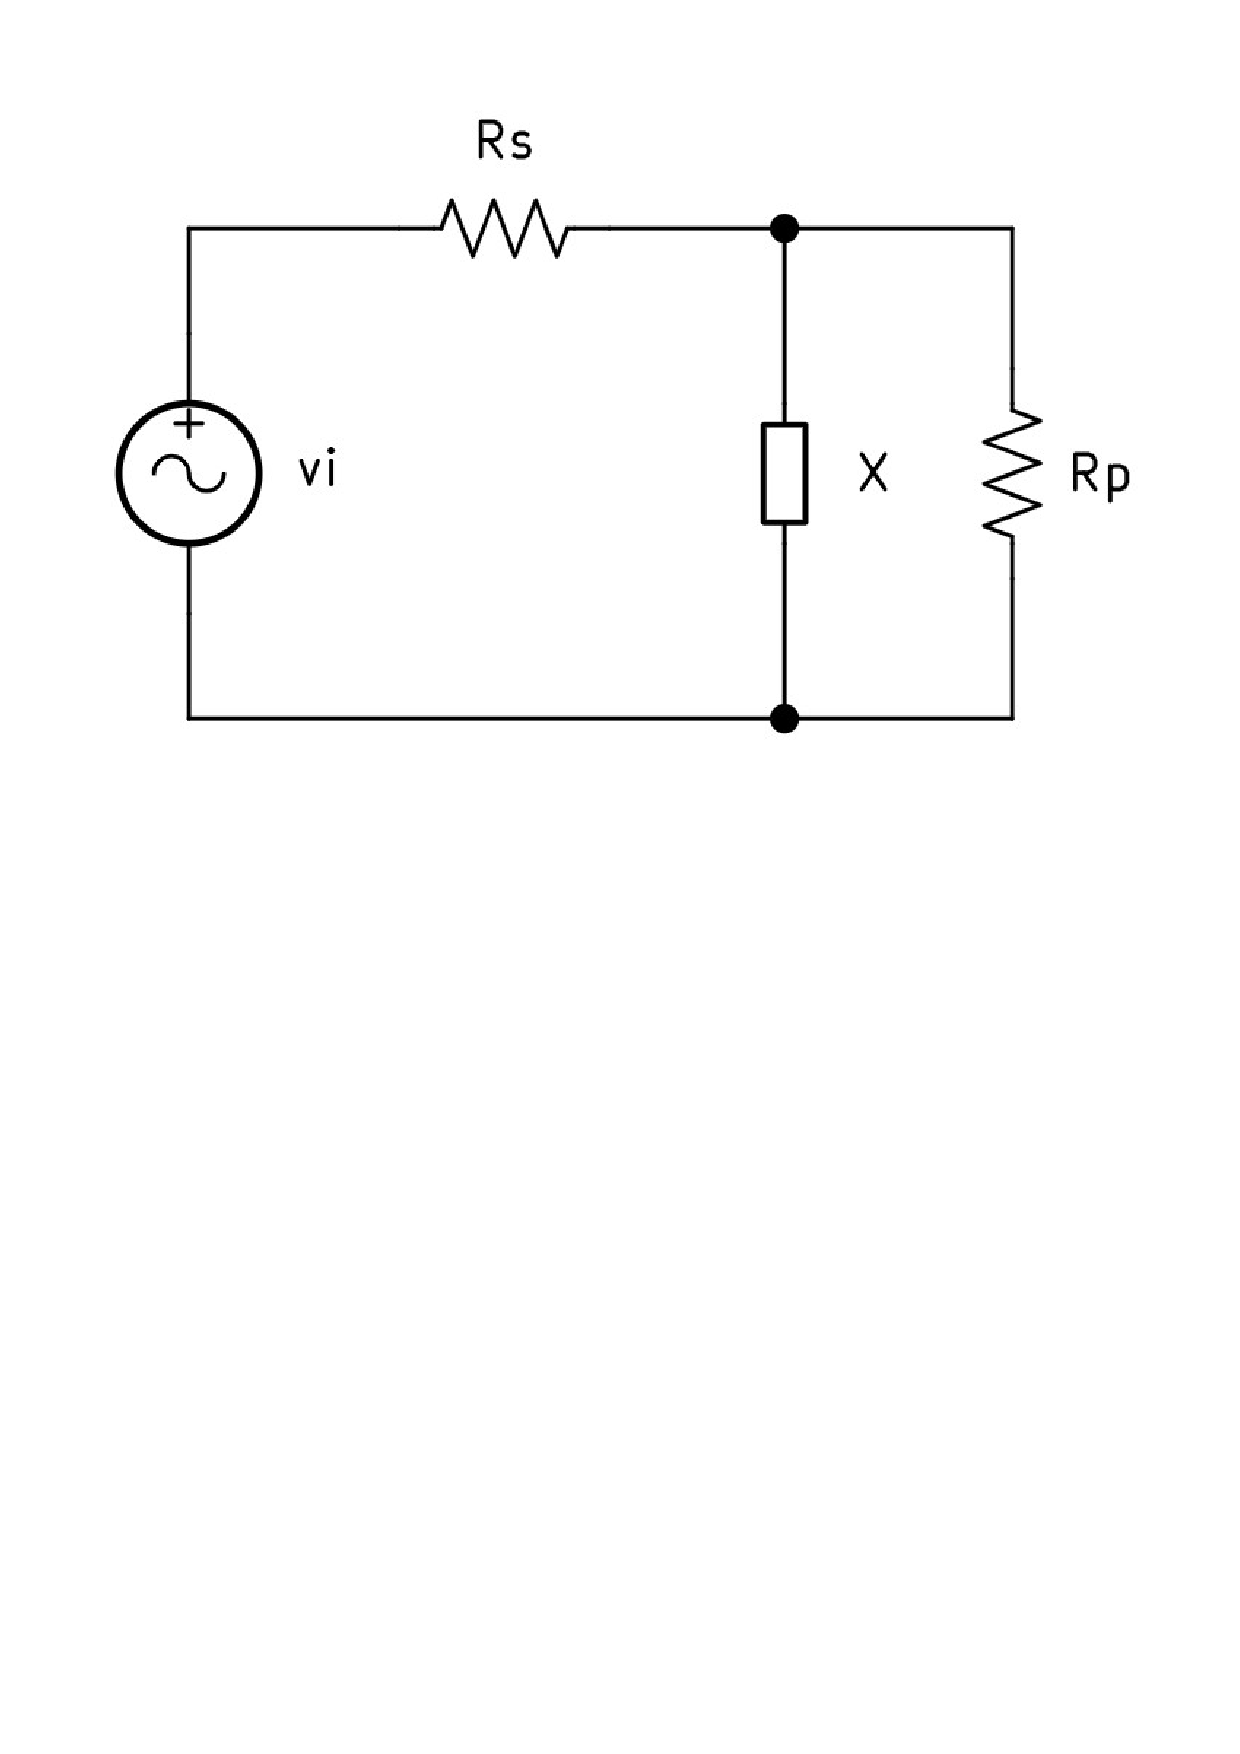
\includegraphics[clip, trim=0 450 0 0, width=0.4\textwidth]{Sections/4_TechnicalAnalysis/Figures/4_1_1_DUTXSeriesParallel.pdf}
    \caption{A simple model of a DUT. The pure reactance X has a series resistance and a parallel resistance.}
    \label{fig:4_1_5_DUTXSeriesParallel}
\end{figure}

If the reactance on figure \refq{fig:4_1_5_DUTXSeriesParallel} is a capacitor then then parallel resistance $R_p$ will, typically, be a large value while the series resistance $R_s$ is small. Eq \refq{eq:4_1_1_CapCurrent5} in section \refq{subsec:Reactance} states that capacitance is inversely proportional to capacitive reactance, so \textit{small} capacitors cause \textit{large} reactance and vice versa. \textit{Small} capacitors are typically used in filter and RF applications where power dissipation in the series resistance is less interesting than the leakage resistance ($R_p$) in the capacitor so it makes sense to model the impedance as a parallel circuit and disregard the series resistance. The series resistance for $large$ filter capacitors in power supply applications will have an impact on the power supplies overall efficiency and the leakage resistance is of less import. In this case it makes sense to model the impedance as a series circuit. The two arrangements that can be used to characterize the DUT is shown on figure \refq{fig:4_1_5_DUTXSeriesParallelMode}.

\begin{figure}[H]
    \centering
    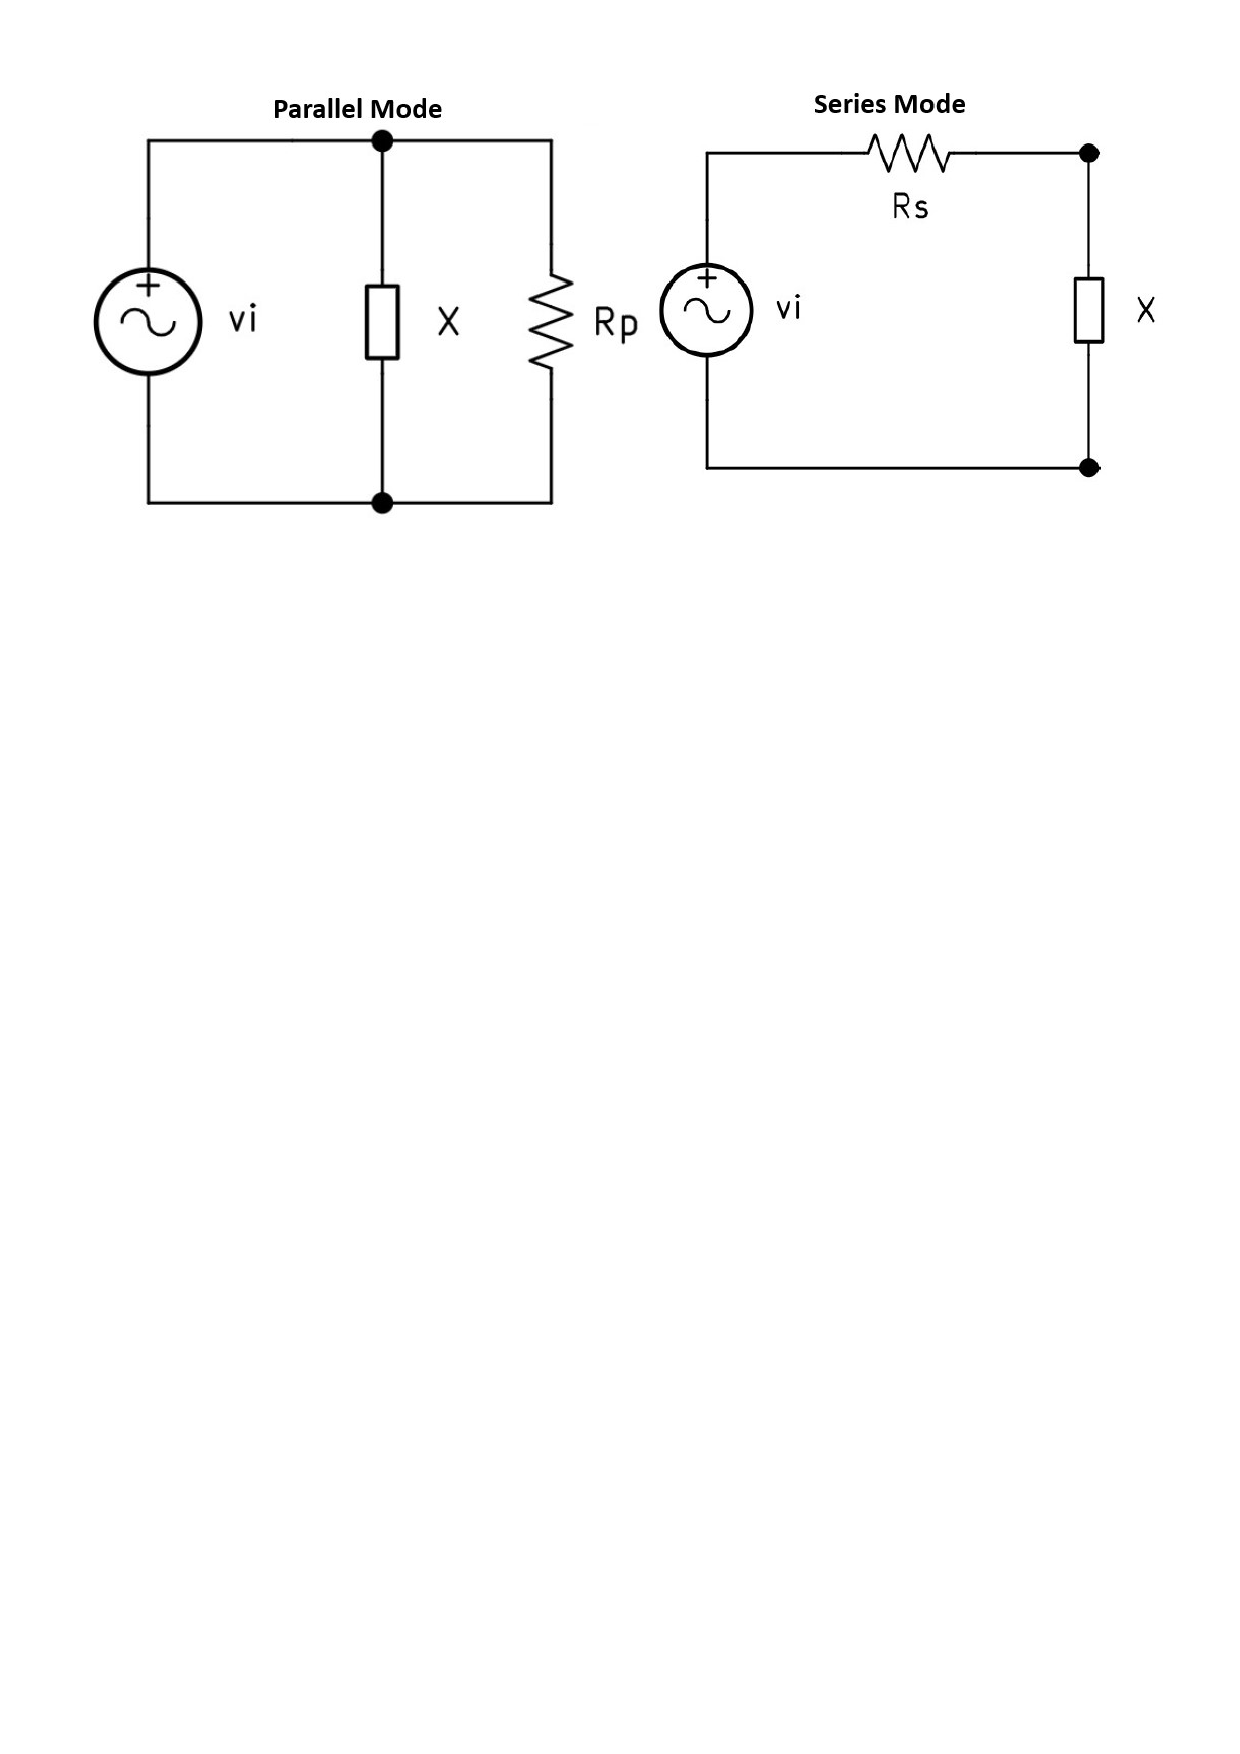
\includegraphics[clip, trim=0 550 0 0, width=0.8\textwidth]{Sections/4_TechnicalAnalysis/Figures/4_1_5_SeriesParallelMode.pdf}
    \caption{The two models that could be used for the DUT. The impedance measured can be fitted to either of them depending on the situation.}
    \label{fig:4_1_5_DUTXSeriesParallelMode}
\end{figure}

Assuming $\bar v$ and $\bar i$ from section \refq{sec:ImpedanceAnalysis} has been measured. The series model can be fitted to the impedance as $\bar Z =|\bar Z| \cdot \mathrm e^{\pm j\phi}$ where Rs and X will be the real and imaginary parts of the complex impedance as shown in eq \refq{eq:4_1_5_SeriesModel1}.

\begin{equation}\label{eq:4_1_5_SeriesModel1}
    \begin{split}
        R_s =& \Re(|\bar Z| \cdot \mathrm e^{\pm j\phi}) = |\bar Z| \cdot cos(\phi)\\
        X =& \Im(|\bar Z| \cdot \mathrm e^{\pm j\phi}) = \pm j\cdot |\bar Z| sin(\phi) 
    \end{split}
\end{equation}

These values in eq \refq{eq:4_1_5_SeriesModel1} can be used to fit the impedance to the series model shown on figure \refq{fig:4_1_5_DUTXSeriesParallelMode}. The admittance of the parallel arrangement can be written as in eq \refq{eq:4_1_5_ParallelModel1}.
\begin{equation}\label{eq:4_1_5_ParallelModel1}
    \bar Y = \frac{|\bar i| [cos(\phi_1) + j\cdot sin(\phi_1)]}{|\bar v| [cos(\phi_0) +j\cdot sin(\phi_0)]}
\end{equation}
Again, like in section \refq{sec:ImpedanceAnalysis}, it is assumed that the reference voltage waveform has $\phi = 0$. This simplifies eq \refq{eq:4_1_5_ParallelModel1} to \refq{eq:4_1_5_ParallelModel2}.
\begin{equation}\label{eq:4_1_5_ParallelModel2}
    \bar Y = \frac{|\bar i| [cos(\phi_1) + j\cdot sin(\phi_1)]}{|\bar v|}
\end{equation}
Simplifying eq \refq{eq:4_1_5_ParallelModel2} and defining that $|\bar Y| = \frac{|\bar i|}{|\bar v|}$to rectangular form gives eq \refq{eq:4_1_5_ParallelModel3}.
\begin{equation}\label{eq:4_1_5_ParallelModel3}
    \bar Y = |\bar Y| cos(\phi_1) + j |\bar Y| sin(\phi_1)
\end{equation}
The real part of the complex admittance is the conductance $G$ while the imaginary part is the susceptance $B$ as shown in eq \refq{eq:4_1_5_ParallelModel4}.
\begin{equation}\label{eq:4_1_5_ParallelModel4}
    \begin{split}
        G =& \Re(|\bar Y| cos(\phi_1) + j |\bar Y| sin(\phi_1)) = |\bar Y| \cdot cos(\phi)\\
        jB =& \Im(|\bar Y| cos(\phi_1) + j |\bar Y| sin(\phi_1)) =  j\cdot |\bar Y| sin(\phi)  
    \end{split}
\end{equation}

The admittance $\bar Y$ can be converted to impedance as shown in eq \refq{eq:4_1_5_ParallelModel4} as impedance is the reciprocal of admittance $Z = \frac{1}{Y}$ as shown in eq \refq{eq:4_1_5_ParallelModel5}.
\begin{equation}\label{eq:4_1_5_ParallelModel5}
    \bar Z = \frac{1}{G + jB} =\frac{G-jB}{G^2 + B^2} = \frac{G}{G^2 + B^2} -j\frac{B}{G^2 + B^2}
\end{equation}
Eq \refq{eq:4_1_5_ParallelModel5} and eq \refq{eq:4_1_5_ParallelModel4} can convert a series impedance into a parallel impendance of the forms show on figure \refq{fig:4_1_5_DUTXSeriesParallelMode}. It is important to note how these models only fit for exactly 1 frequency. They must be recalculated if the test frequency is changed.

\section{Typical Impedance Measurement Principles} \label{sec:TypicalMeasPrin}

\subsection{Wheatstone Bridge} \label{ssec:BridgeCircuits}
The Wheatstone bridge has been around since the 1800 hundreds, and was among the very first methods used to characterize an unknown impedance. Originally only used for DC resistance measurements, but with a few modifications it was expanded to characterize impedances as well. 
The circuit can be seen in figure \ref{fig_4_2_WheatstoneBridge}, where $Z_1$ is the unknown device,
 often referred to as the DUT.
 
A null detector is present across the two nodes, this allows the two impedance ratios $Z_1/Z_3$ and $Z_2/Z_4$
to be matched. If there is \SI{0}{\volt} at all times across node b and d, then the ratio of $Z_1/Z_3$ will match that of
 $Z_2/Z_4$, and the
phase angle will be given as $\theta_1 - \theta_2 = \theta_2 - \theta_4$. 

\begin{figure}[H]
    \centering
    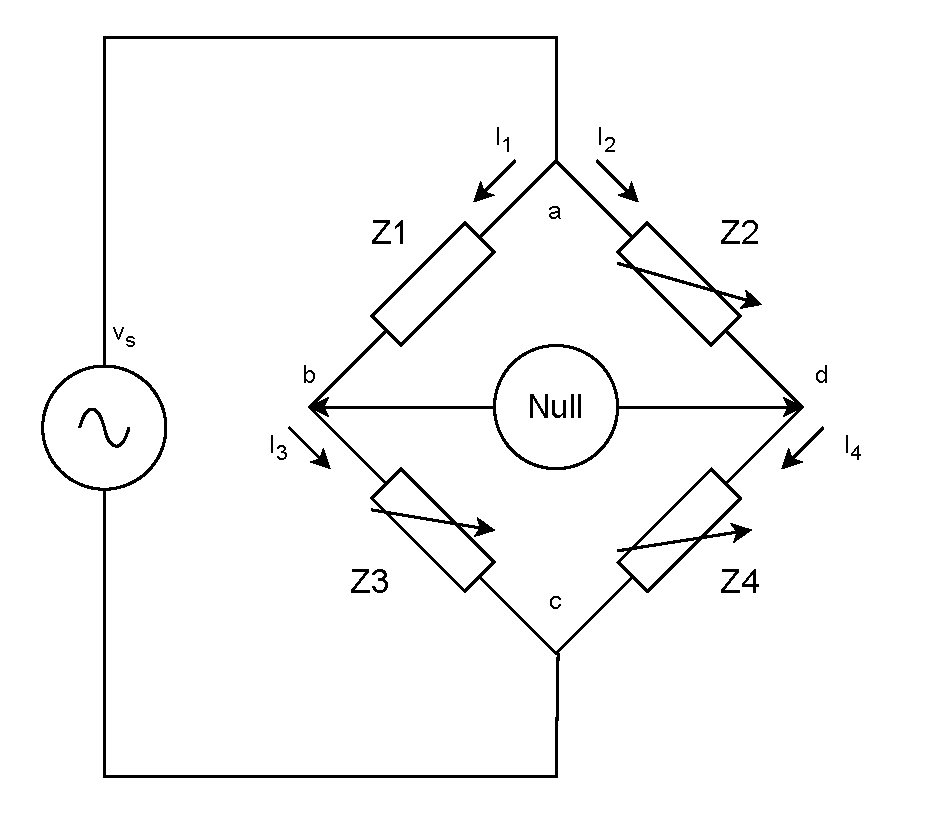
\includegraphics[width=0.75\textwidth]{Sections/4_TechnicalAnalysis/Figures_JFT/WheatstoneBridgeAC.pdf}
    \caption{A typical AC Wheatstone bridge, where Z1 is the device under test.}
    \label{fig_4_2_WheatstoneBridge}
\end{figure}

The relationship between the different impedances can be described by analyzing the bridge. The voltage across $Z_1$ and $Z_2$ can
be described as in equation \ref*{eq:4_2_TopWheatstone}.

\begin{equation}
    \begin{split}
        \label{eq:4_2_TopWheatstone}
        i_1 &= \frac{v_s-v_1}{Z_1} \Rightarrow -i_1 Z_1 +v_s = v_1 \\
        i_2 &= \frac{v_s-v_1}{Z_2} \Rightarrow -i_2 Z_2 + v_s = v_2
    \end{split}
\end{equation}

Under the assumption that the null detector reads zero, and the same voltage is present at node b and d, then the voltage
across $Z_1$ must be equal to that across $Z_2$. From this equation \ref{eq:4_2_TopWheatStone2} can be constructed, showing the
relationship between currents and impedances for the top most resistors of the bridge.

\begin{equation}
    \begin{split}
        \label{eq:4_2_TopWheatStone2}
        v_1 &= v_2 \Rightarrow -i_1 Z_1 +v_s = -i_2 Z_2 + v_s \\
        i_1 Z_1 &= i_2 Z_2 \Rightarrow \frac{i_2}{i_1} = \frac{Z_1}{Z_2}
    \end{split}
\end{equation}

In much the same way, the lower half of the bridge can be described as seen in equation \ref{eq:4_2_BotWheatstone}

\begin{equation}
    \label{eq:4_2_BotWheatstone}
    \frac{i_4}{i_3} = \frac{Z_3}{Z_4}
\end{equation}

A proper null detector will not interfere with the circuit it is measuring, so no current should flow in to or out of the
null detector, meaning that $i_1$ must equal $i_3$ and $i_2 = i_4$, as the components are in series. Under this assumption, it can be
shown that the unknown impedance $Z_1$ and its phase angle can be found from the 3 other know impedances and phase angles, as shown
in equation \ref{eq:4_2_MatchedWheatstone}.

\begin{equation}
    \begin{split}
        \label{eq:4_2_MatchedWheatstone}
        \frac{i_2}{i_1} &= \frac{i_4}{i_3} \Rightarrow \frac{Z_1}{Z_2} = \frac{Z_3}{Z_4} \Rightarrow \frac{Z_1}{Z_3} = \frac{Z_2}{Z_4} \\
        \frac{|Z_1|\e^{j\theta_1}}{|Z_3|\e^{j\theta_3}} &= \frac{|Z_2|\e^{j\theta_2}}{|Z_4|\e^{j\theta_4}}
        \Rightarrow \frac{|Z_1|}{|Z_3|}\e^{j\left(\theta_1-\theta_3\right)} = \frac{|Z_2|}{|Z_4|}\e^{j\left(\theta_2-\theta_4\right)} \\
        \\
        \Rightarrow \frac{|Z_1|}{|Z_3|} &= \frac{|Z_2|}{|Z_4|} \quad and \quad \theta_1-\theta_3 = \theta_2-\theta_4 \\
        \Rightarrow |Z_1| &= \frac{|Z_2|\cdot|Z_3|}{|Z_4|} \quad and \quad \theta_1 = \theta_2+\theta_3-\theta_4
    \end{split}
\end{equation}

The AC Wheatstone bridge has proven itself to be highly accurate, but is somewhat frequency limited, and expensive, as it requires a
vast arsenal of stable and well known capacitors and resistors to be used for the 3 adjustable impedances. This is something that
is typically found in a metrology grade laboratory and not in an instrument.


\subsection{I-V Method} \label{ssec:IVMethod}
The I-V method or current voltage method, has already been shortly introduced in section \ref{sec:MeasureReactiveComponents}, here it was realized by the use of a function generator and an oscilloscope. In this chapter, the I-V method will however be introduced in a more broad spectrum, that is to say, the general principle of the method will be outlined.

In general, two principles of the I-V method are implemented in the industry, either the I-V method or the RF I-V method. The I-V method offers good accuracy 
and a broad bandwidth, from a few hertz to about \SIQ{100}{\mega\hertz}. The RF I-V method uses RF principles such as directional couplers and extends the bandwidth up to about \SIQ{3}{\giga\hertz}, it is however not suitable for frequencies below the mega hertz region\cite{Keysight_Impedance}. This chapter will solely focus on the I-V method as the RF frequency range is not of interest to this project.

The principle of the I-V method is simple; measure current and voltage, and determine the angle between them. This can be implemented in numerous different ways, using coupled inductors to measure the current, or a series shunt where the voltage-drop can be measured across, to name a few. 

\begin{figure}[H]
    \centering
    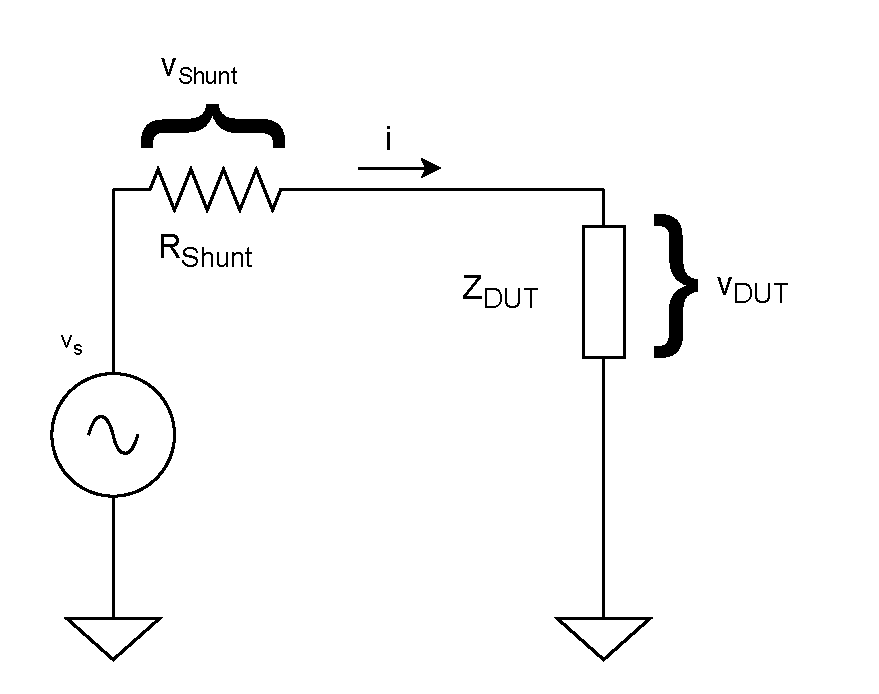
\includegraphics[width=0.75\textwidth]{Sections/4_TechnicalAnalysis/Figures_JFT/IV_Method.pdf}
    \caption{The I-V Method implemented with a current shunt to measure the current}
    \label{fig_4_2_IVMethod}
\end{figure}

The principle of the I-V method can be seen in figure \refq{fig_4_2_IVMethod}. The current in the system can be described by an amplitude and phase, as can the voltage, as seen in equation \ref{eq:4_2_2_IVVectors}, where $v$ is the voltage across the DUT and $i$ is the current through it. It is assumed that the current is the same through the shunt and the DUT.

\begin{equation}
    \label{eq:4_2_2_IVVectors}
    \begin{split}
        \bar{i} & = |i|\cdot\e ^{j\theta_i} \Rightarrow \bar{i} = \frac{|v_{shunt}|}{R_{shunt}}\e ^{j\theta_{v\:shunt}}\\
        \bar{v_{DUT}} & = |\bar{v_{DUT}}| \cdot\e ^{j\theta_{v\:DUT}}
    \end{split}
\end{equation}

The impedance can then be calculated from the two voltages of the system, i.e. the shunt voltage and the DUT voltage, as seen in equation \ref{eq:4_2_2_Impedance}.

\begin{equation}
    \label{eq:4_2_2_Impedance}
    \begin{split}
        Z & = \frac{v_{DUT}}{i} \Rightarrow \bar{Z} = \frac{|v_{DUT}| \cdot\e ^{j\theta_{v\:DUT}}}{\frac{|v_{shunt}|}{R_{shunt}}\e ^{j\theta_{v\:shunt}}} \\
        \bar{Z} & = \frac{|v_{DUT}|\cdot R_{shunt}}{|v_{shunt}|}\cdot \e ^{j\left(\theta_{v\:DUT}-\theta_{v\:shunt}\right)}
    \end{split}
\end{equation}

This is the I-V method in its simplest form. The shunt used is however required to be swapped depending on the DUT, as a small shunt would be poorly suited to measure small currents. In practice, compensation elements can also be required to ensure stability, as some systems can become unstable under large capacitive loads.
\subsection{Auto Balancing Bridge} \label{ssec:AutoBalanceBridge}
The auto balancing bridge is build around the principle of feedback, and is often implemented by the use of an operational amplifier or op-amp. The bandwidth is however somewhat limited when an op-amp is used to implement this technique, to work around this, this principle is sometimes implemented by the use of a null detector, a phase sensitive detector and a phase and amplitude variable generator. This is a rather complex circuitry, and this chapter will only introduce the principle of the auto balancing bridge, and as such treat it like 
an op-amp circuit.

\begin{figure}[H]
    \centering
    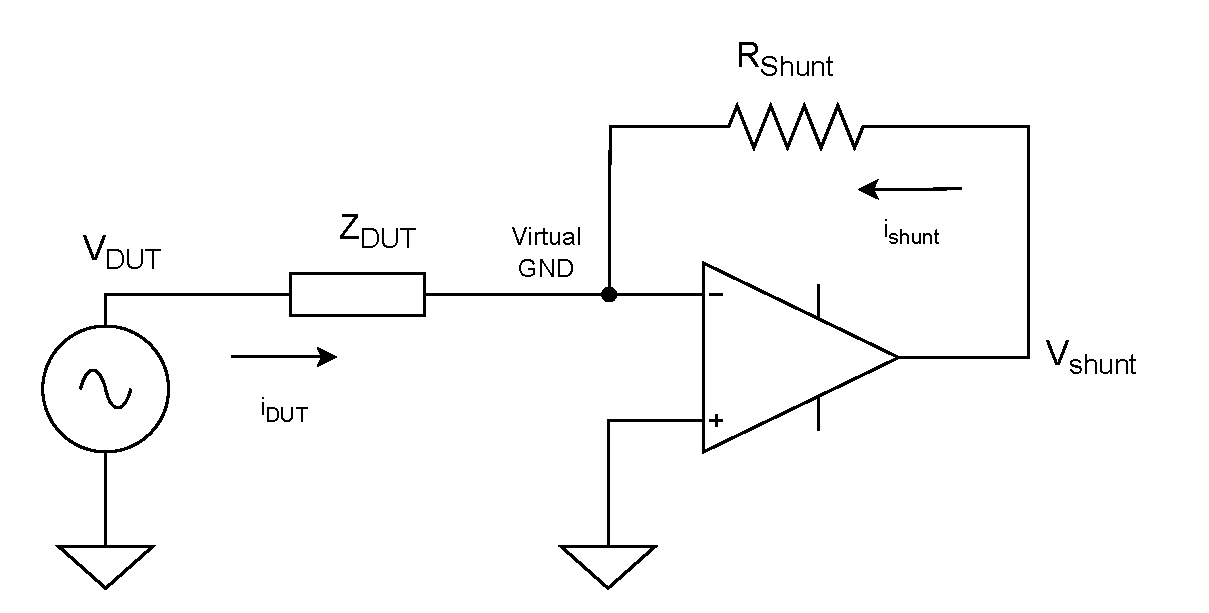
\includegraphics[width=0.75\textwidth]{Sections/4_TechnicalAnalysis/Figures_JFT/AutoBalanceBridge.pdf}
    \caption{The general principle of the auto balancing bridge circuit.}
    \label{fig_4_2_AutoBalanceBridge}
\end{figure}

The principle can be seen on figure \ref{fig_4_2_AutoBalanceBridge}, where the inverting input of the op-amp, under ideal assumptions, will be a virtual ground node, thus the voltage across the shunt can simply be measured at the output of the op-amp. Likewise the DUT voltage can also be measured at the node named $V_{DUT}$. This has the advantage that no differential measurements needs to be made. Another
advantage of this circuit is that the input capacitance of the circuit that will measure both the DUT and shunt voltage will be connected
to a low impedance source, i.e. the excitation source and the op-amp output. This means that these parasitic capacities will have a minimum effect on the circuit, and as such this topology is amongst the most precise methods used in impedance analyzers.

It should be noted, that the circuit is configured in an inverting configuration, such that the current measured, as a function of $V_{Shunt}$ will be \SIQ{180}{\degree} phase shifted, compared to the actual DUT current. The circuit is easily analyzed, as an inverting op-amp, as seen in equation \ref{eq:4_2_3AutoBalanceBridge1}.
\begin{equation}
    \label{eq:4_2_3AutoBalanceBridge1}
    \begin{split}
        \frac{v_o}{v_i} &= -\frac{R_{Shunt}}{Z_{DUT}}\\
        v_{DUT} &= v_i \qquad v_{Shunt} = v_o \\
        \Rightarrow Z_{DUT} &= -\frac{R_{Shunt}\cdot v_{Shunt}}{v_{DUT}}
    \end{split}
\end{equation}
equation \ref{eq:4_2_3AutoBalanceBridge1} does however not paint the full picture, as the voltages are complex vectors. Assuming that the phase of the source voltage will not change, equation \ref{eq:4_2_3AutoBalanceBridge1} can be expanded by modeling 
the shunt voltage as a voltage and a phase

\begin{equation}
    \label{eq:4_2_3AutoBalanceBridge2}
    \begin{split}
        \vec{Z_{DUT}} &= -\frac{R_{Shunt}\cdot \vec{v_{Shunt}}}{\vec{v_{DUT}}} \\
        \Rightarrow \vec{Z_{DUT}} &= -\frac{R_{Shunt}\cdot |\vec{v_{Shunt}}|\cdot\e ^{j\theta}}{|\vec{v_{DUT}|}} \\
        \Rightarrow \vec{Z_{DUT}} &= \frac{R_{Shunt}\cdot |\vec{v_{Shunt}}|\cdot\e ^{j\theta}}{|\vec{v_{DUT}|}} \cdot \e ^{-j\pi} \\
        \Rightarrow \vec{Z_{DUT}} &= \frac{R_{Shunt}\cdot |\vec{v_{Shunt}}|\cdot\e ^{j\theta}\cdot \e ^{-j\pi}}{|\vec{v_{DUT}|}}  \\
        \Rightarrow \vec{Z_{DUT}} &= \frac{R_{Shunt}\cdot |\vec{v_{Shunt}}|\cdot\e ^{j(\theta-\pi)}\cdot}{|\vec{v_{DUT}|}}
    \end{split}
\end{equation}

This topology is widely used in precision impedance measurements, especially for frequencies up to a few hundred kilo hertz, at higher frequencies, the op-amps gain tends to reduce too much to produce precise results.
\section{Summary} \label{sec:TechAnalSum}
The technical analysis has introduced varies topologies used in the industry as well as what impedance is, and different ways it can
be described. The reasoning for the somewhat extensive derived quantities section is that many manufacturers of electrical components
states different quantities, some mention D or dissipation factor, some Q, some loss tangent, and some none at all. Thus it is
imperative that these different quantities are introduced, as they are essential in what the solution must undertake.

This chapter introduces these varies elements such that a conclusion upon what methods can be used to answer the problem statement can
be drawn.
\chapter{System Requirements} \label{ch:SystemRequirements}
The user segment that this project is interested in, is the hobbyist segment. The hobbyist segment is anyone with an interest in developing electronic circuits, whether or not they have a technical or engineering background. The hobbyist segment is interested in more capable impedance analyzers than what is available in their price range as seen in section \ref{sec:ProfessionalMarketDemand}. This section has compiled a list of system requirements for an impedance analyzer that will be developed in this project. The requirements are based on the market demands in section \ref{sec:ProfessionalMarketDemand} and the currently available functions in high-end impedance analyzers shown in section \ref{sec:CommercialImpedanceAnalyzerCapabilities}, and the personal requirements from the authors of this report. 
\begin{table}[H]
    \begin{tabular}{|m{3.5em}|m{15em}|m{15em}|}
    \hline
      \textbf{ID} &   \textbf{Description}       & \textbf{Requirement}  \\ \hline
      §1 & Frequency range &    \SIQ{50}{\hertz} - \SIQ{1}{\mega\hertz} \\ \hline
      §2 & Impedance fit$^1$ & Series and parallel mode \\\hline 
      §3 & Impedance range & $\SIQ{10}{\milli\ohm}\leq|Z|\leq\SIQ{100}{\mega\ohm}$ \\ \hline
      §4 & $|Z|$, Modulus accuracy$^2$& $A_Z(f_m, Z_m)$ \\ \hline
      §5 & $\angle\phi$, Accuracy of argument$^3$ & $A_\phi(f_m, Z_m)$ \\ \hline
      §6 & Test voltage range & \SIQ{10}{\milli\volt}$_{pp}$ - \SIQ{5}{\volt}$_{pp}$ \\ \hline
      §7 & Maximum test current & \SIQ{100}{\milli\ampere}$_{pp}$ \\ \hline
      §8 & DC bias voltage range & \SIQ{0}{\volt}DC - \SIQ{20}{\volt}DC \\ \hline
      §9 & Parameters of DUT & $L/C/R/Q/D/R_s/R_p/Z\theta$ \\ \hline
      §10 & Parameter sweep & Can perform \newline frequency and bias sweep \\ \hline
      §11 & Frequency sweep range$^4$ & \SIQ{50}{\hertz} - \SIQ{1}{\mega\hertz} \\ \hline
      §12 & Maximum frequency \newline sweep points$^5$ & 10000 points in a sweep \\ \hline
      §13 & Maximum bias sweep points$^6$ & 100 Points \\ \hline
      §14 & Binning & Can do component binning \\ \hline
      §15 & Histogram & Can plot a histogram$^7$ \\ \hline
      §16 & Plots & Can plot all parameters vs. \newline frequency and bias voltage \\ \hline
      §17 & Interface & Minimum 7" touchscreen \\ \hline
      §18 & DUT connection & 4-wire kelvin connection \\ \hline
      §19 & Data export & Can export data to CSV file \newline via UART. \\ \hline
    \end{tabular}
    \caption*{
      \raggedright
      $\mathbf{^1}$ Impedance fit refers to the model used to represent the impedance, see section \refq{subsec:SeriesToParallel}.\\
      $\mathbf{^2}$ The accuracy of the measured impedance magnitude, see section \ref{sec:ModulusArgumentAccuracy}. \\
      $\mathbf{^3}$ The accuracy of the phase angle of the measured impedance, see section \ref{sec:ModulusArgumentAccuracy}. \\
      $\mathbf{^4}$ The maximum range of a frequency sweep. \\
      $\mathbf{^5}$ The maximum points that a frequency sweep can contain. \\
      $\mathbf{^6}$ The maximum points that a bias voltage sweep can contain. \\
      $\mathbf{^7}$ Capable of measuring and saving multiple component values, such that a histogram of the components can be shown. \\
    }
    \caption{Table to test captions and labels.}
    \label{tab:5_SystemRequirements}
  \end{table}

\section{Modulus and Argument Accuracy} \label{sec:ModulusArgumentAccuracy}
The requirement of both impedance magnitude accuracy and phase accuracy, or modulus and argument accuracy will be described in more detail
in this section. This is done based on the specifications from commercially available impedance analysers, as the 
requirements are based upon these.

The requirements for modulus and argument accuracy are based on the R\&S LCX-200, given that the scope of this project is to
research and develop an impedance analyser at a lower price point, the specifications are looser than that of the LCX-200.

Section \ref{sec:CommercialImpedanceAnalyzerCapabilities} has shown how the accuracy of impedance analyzer degrade as they deviate from
their ideal operating point, often around \SIQ{1}{\kilo\hertz} and \SIQ{1}{\kilo\ohm}. The specifications given here is based upon this
principle and as a result it is given as a continoues two variable function, both for modulus and argument.

The required measurement accuracy of the impedance magnitude is given as a function with two input variables as seen in equation
\refq{eq:5:A_Z}
\begin{equation}
  \begin{split}
      \label{eq:5:A_Z}
      A_Z(f_m, Z_m) & \leq \left(\pm 0.1\% + |log_{10}\left( f_m \right)|\cdot0.3\%+ |log_{10}\left( |Z_m| \right)|\cdot0.3\%\right)\\
      f_m & = Measurement \; frequency \; in \; kHz. \\
      Z_m &= Measured \; impedance \; magnitude \; in \; k\Omega.
  \end{split}
\end{equation}

Such that the further away from \SIQ{1}{\kilo\hertz} the test frequency is, the worse the measurement accuracy will be. The same 
is true for the magnitude of the impedance, such that the further away from \SIQ{1}{\kilo\ohm} the measured impedance is, the less
accurate the measurement will be.

An example could be given at $f_ m = \SIQ{100}{\kilo\hertz}$ and measured impedance magnitude of $|Z_m| = \SIQ{10}{\ohm}$. Here the
accuracy of the instrument should be better than \SIQ{1.3}{\%}, as seen from equation \refq{eq:5:A_Z_example}.
\begin{equation}
  \label{eq:5:A_Z_example}
  \begin{split}
    A_Z(100, 0.01) & \leq \pm \left(0.1\% + |log_{10}(100)|\cdot0.3\%+|log_{10}(0.01)|\cdot0.3\% \right)\\
    \Rightarrow A_Z(100, 0.01) & \leq \pm \left( 0.1\% + |2|\cdot0.3\%+|-2|\cdot0.3\% \right) \\
    \Rightarrow A_Z(100,0.01) & \leq \pm \left( 0.1\% + 0.6\% + 0.6\% \right) \Rightarrow A_Z(100,0.01) \leq \pm 1.3\% 
  \end{split}
\end{equation}

The two dimmensional function for modulus accuracy can be seen as two plots in figure \ref{fig_5_ModulusAccuracy}. Here the left plot is with a fixed impedance of \SIQ{1}{\kilo\ohm}
and a sweept frequency from \SIQ{50}{\hertz} to \SIQ{1}{\mega\hertz}, and the right plot is with a fixed frequency of \SIQ{1}{\kilo\hertz} with impedance ranging from \SIQ{10}{\milli\ohm} to \SIQ{100}{\mega\ohm}.


\begin{figure}[H]
  \centering
  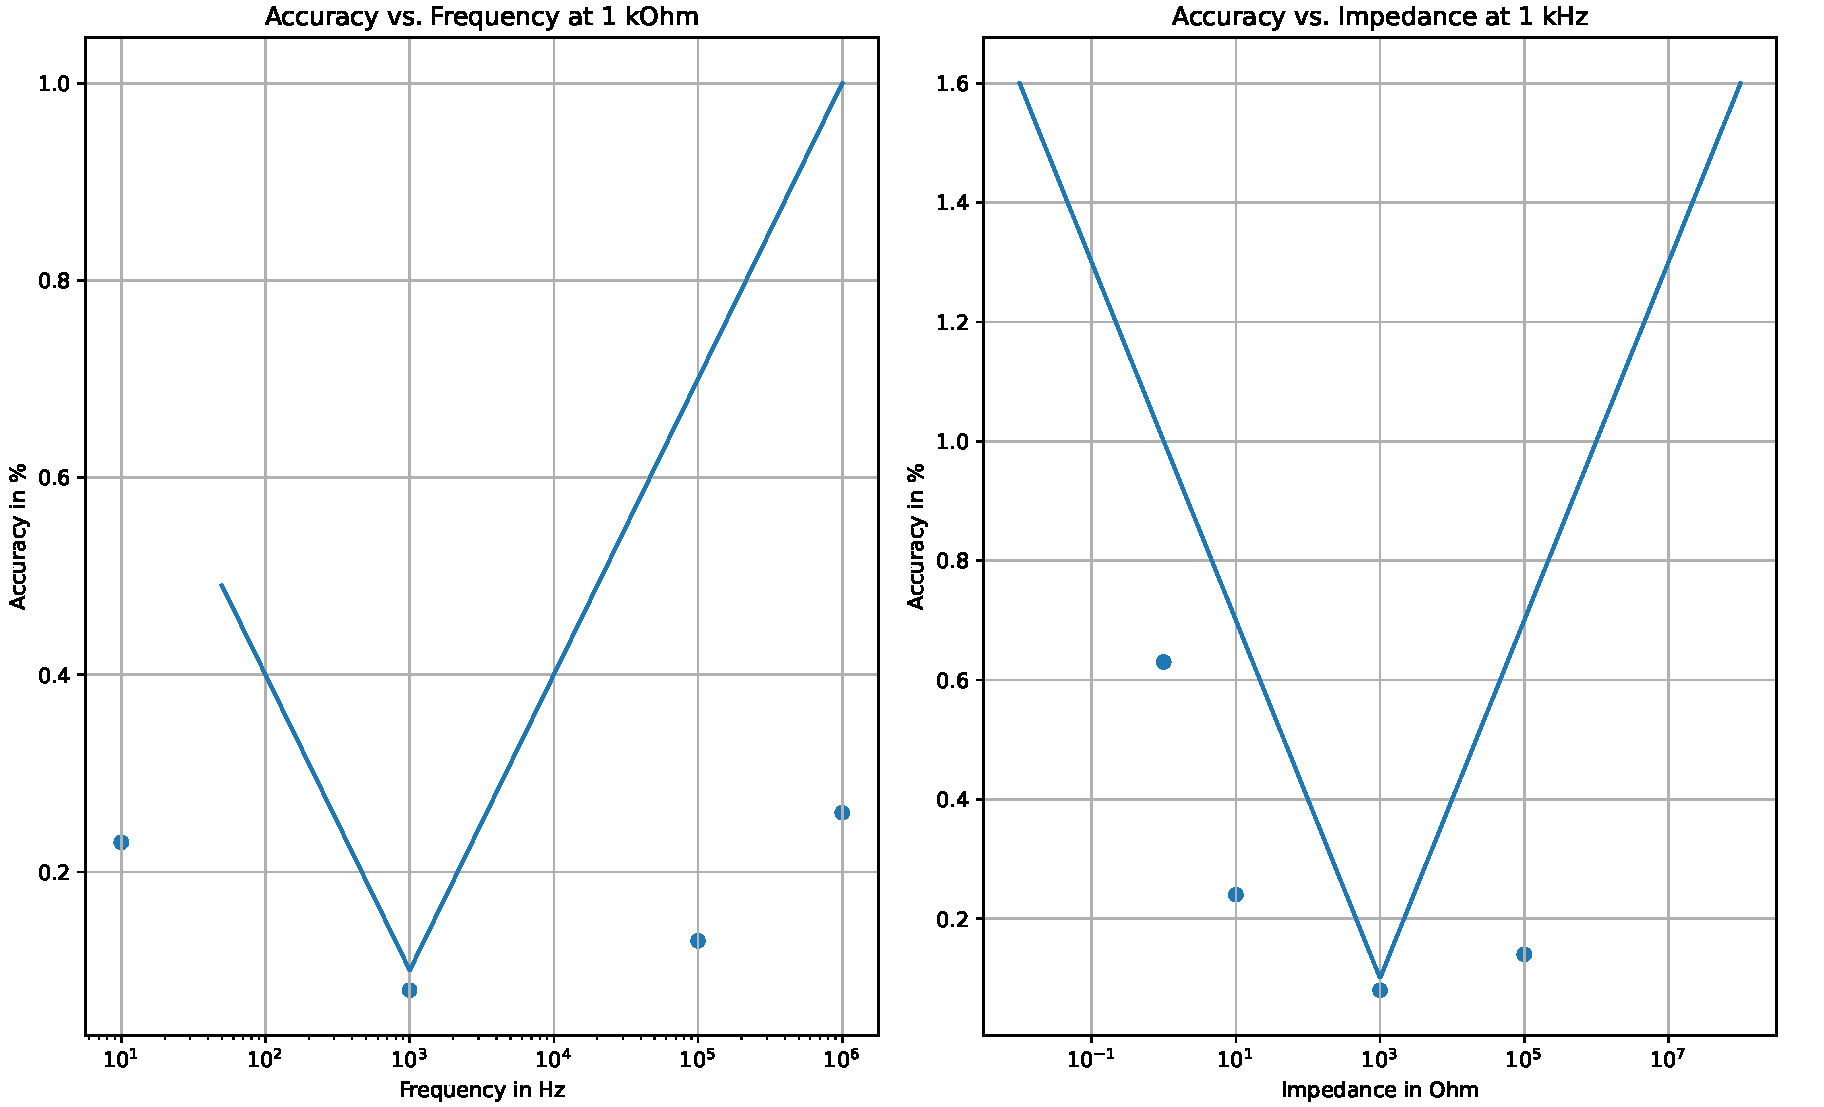
\includegraphics[width=1\textwidth]{Sections/5_SystemRequirements/Figures/ImpedanceSpec.pdf}
  \caption{Plots of the requirement for modulus accuracy, left for fixed impedance, but varying frequency, right with fixed frequency but varying impedance.}
  \label{fig_5_ModulusAccuracy}
\end{figure}

The phase accuracy is given in much the same way as for impedance. The accuracy of the phase will be dependant on the accuracy of the magnitude of the measured impedance, and as such, the phase accuracy in degrees is a function that is dependant on the impedance magnitude accuracy as can be seen in equation \ref{eq:5:A_Phi}.

\begin{equation}
  \begin{split}
    \label{eq:5:A_Phi}
    A_\phi(f_m, Z_m) & \leq \frac{180}{\pi} \cdot \frac{A_Z(f_m,Z_m)}{100} \qquad in \:degrees\\
    f_m & = Measurement \; frequency \; in \; kHz. \\
    Z_m &= Measured \; impedance \; magnitude \; in \; k\Omega.
  \end{split}
\end{equation}

Following on the previous example with an impedance of \SIQ{10}{\ohm} at a frequency of \SIQ{100}{\kilo\hertz} the impedance magnitude accuracy requirement is \SIQ{1.3}{\%} the phase
angle accuracy would be $A_(100,0.01) \leq (180/\pi)\cdot(1.3/100) = \SIQ{0.745}{\degree}$. This two variable function can also be shown as a side by side plot as seen in figure \ref{fig_5_PhaseAccuracy}.

\begin{figure}[H]
  \centering
  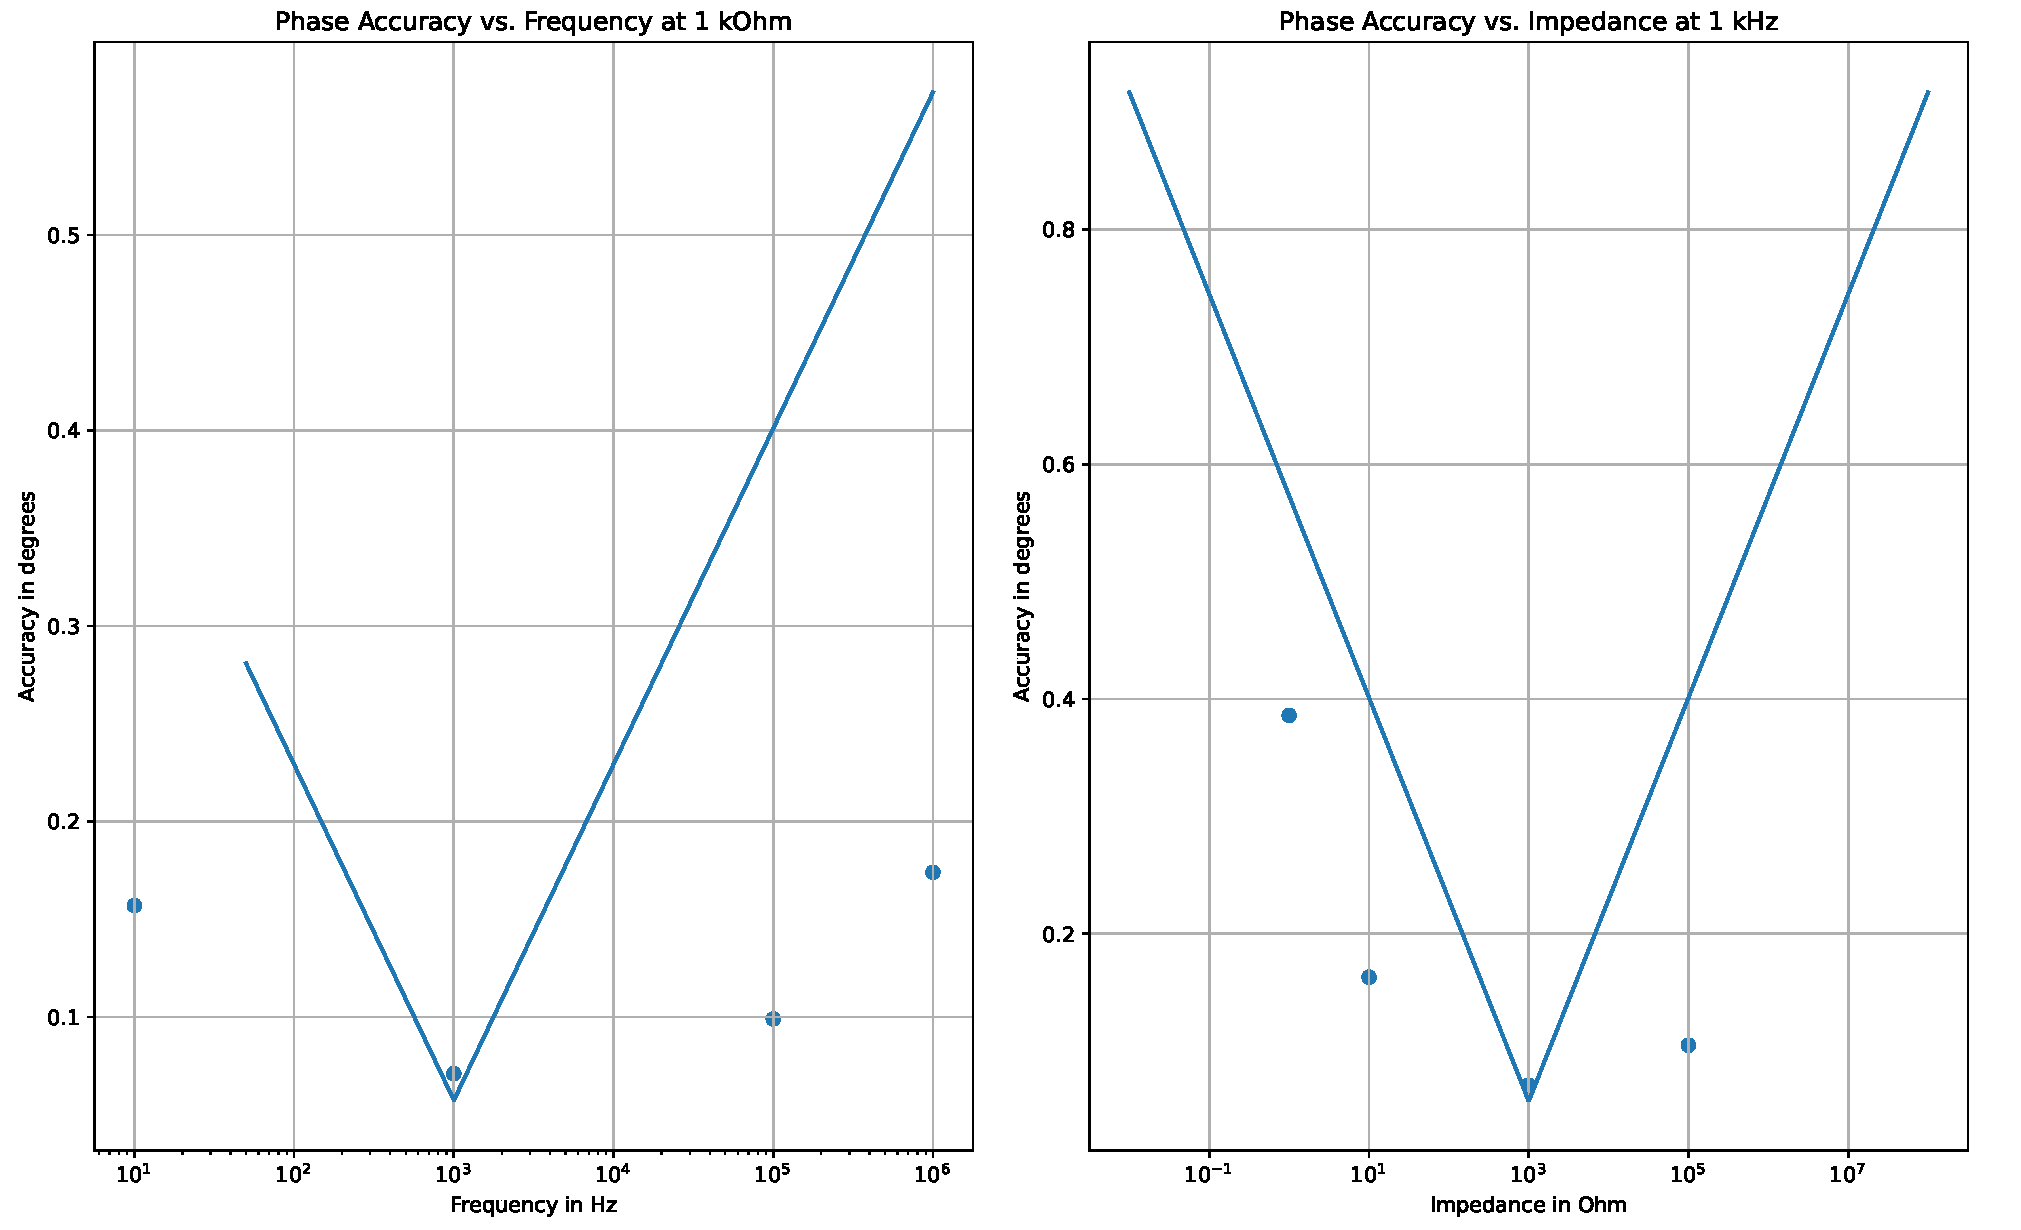
\includegraphics[width=1\textwidth]{Sections/5_SystemRequirements/Figures/PhaseSpec.pdf}
  \caption{Plots of the requirement for argument accuracy, left for fixed impedance, but varying frequency, right with fixed frequency but varying impedance.}
  \label{fig_5_PhaseAccuracy}
\end{figure}
\section{Binning} \label{sec:5_1_Binning}
Binning is a principle often used when sorting components. It allows a target value and tolerance to be programmed in to the device. For example, if on wishes to sort 100 nF capacitors in to different bins of accuracy, the target value is set to 100 nF, bins might be \SIQ{1}{\%} and \SIQ{5}{\%}. Whenever a component is measured, the instrument will indicate what bin the component belongs to, if it is within the less than \SIQ{1}{\%} error bin, this will be indicated, if it is within \SIQ{5}{\&} error bin this will be indicated and so on.
\section{Histogram} \label{sec:5_1_Histogram}

%System Architecture
\chapter{System Architecture} \label{ch:SysArchitecture}

The impedance analyzer that is developed in this project will follow the IV-method described in section \refq{ssec:IVMethod} in order to acquire the DUT current and voltage waveforms so they can be converted into the derived quantities of interest. A proposal for a system architecture for the impedance analyzer has been made. The proposal is based on the system requirements listed in chapter \refq{ch:SystemRequirements} along with the method and principles established in chapter \refq{ch:TechnicalAnalysis}. The architecture can be seen on the block diagram on figure \refq{fig_6_SysArchitecture}. This chapter will introduce the systems functional principle.

\begin{figure}[H]
    \centering
    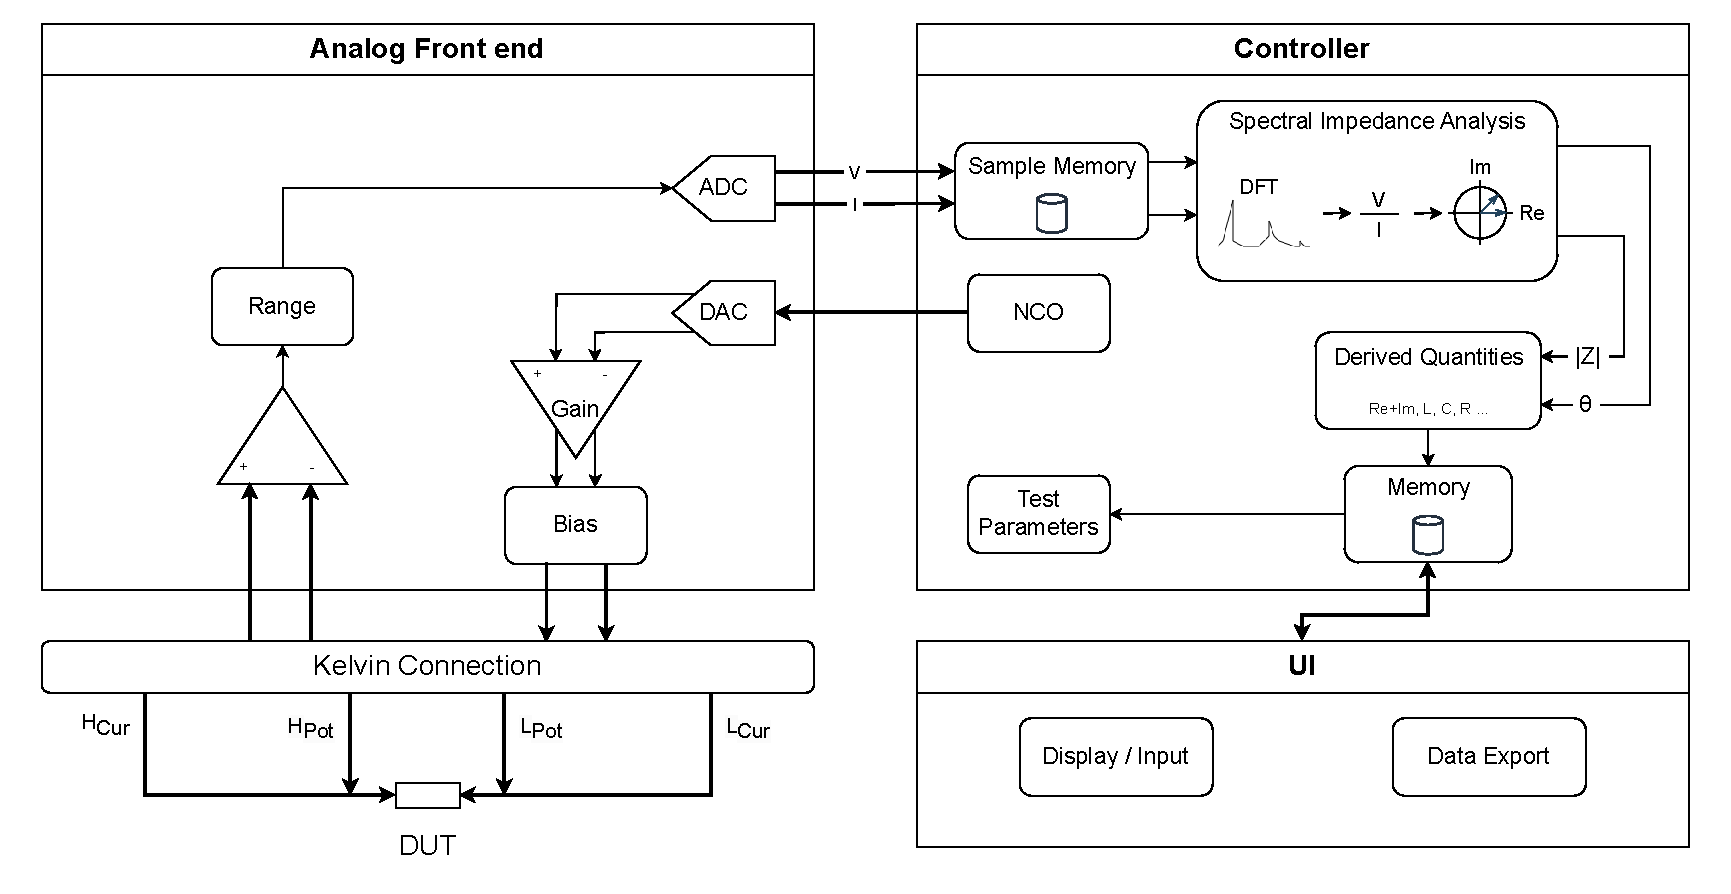
\includegraphics[clip, trim=18 0 18 0,width=1.0\textwidth]{Sections/6_SystemArchitecture/Figures/SystemArchitecture.pdf}
    \caption{The proposed system architecture for the impedance analyzer designed in this document. An analog front end will measure DUT voltage and current, 
    this will then undergo spectral analysis, such that phase and magnitude information can be obtained and used to calculate all derived quantities. A user can set the test parameters using a UI, these parameters in turn will determine DAC settings, range and sample rate.}
    \label{fig_6_SysArchitecture}
\end{figure}

The heart of the impedance analyzer lies in the Analog Front End whose purpose is to generate the test signals through DA-conversion while simultaneously acquiring the resulting DUT voltage and DUT current waveforms with AD-conversion. The DA- and AD-conversion is controlled by a sample control system. The sample control system will generate the required inputs for the DAC and it will take the samples from the two AD-converters and store them in sample memory. The sample control system will interface with a main processor. The main processors primary purpose is to retrieve the samples from the sample memory and perform all the necessary calculations on those samples in order to get the derivived quantities described in section \refq{subsec:DerivedQuantities}. When it has done the calculations it will transmit the results to a user interface - a display. The user interface will let the user set the test parameters, through a touch screen, and it will display the test results to the user.

The project team have discussed, extensively, the choice of digital platform and architecture for this system before arriving at the FPGA and Microprocessor combo shown on figure \refq{fig_6_SysArchitecture}. These considerations can be seen in appendix \refq{App:MicrocontrollerConsiderations}.

The system architecture on figure \refq{fig_6_SysArchitecture} has been split into separate modules in order to develop them in parallel. Each of the modules will be described in detail in the following subsections along with their specifications and required interfaces.

\section{Analog Front End} \label{sec:AnalogFrontEnd}

The analog front is a critical part of the impedance analyzer. The module is internally split into two major sections; a test signal generator and a sampling circuit. The module will generate test signals for the DUT with a digital-to-analog converter (DAC) and then acquire and sample the resulting DUT current and voltage waveforms with an analog-to-digital converter (ADC). A snippet of the analog front end can be seen on figure \refq{fig_6_1_AnalogFrontEnd}. Here it can also be seen that the Analog Front End will connect to the DUT using a 4 wire Kelvin connection.

\begin{figure}[H]
    \centering
    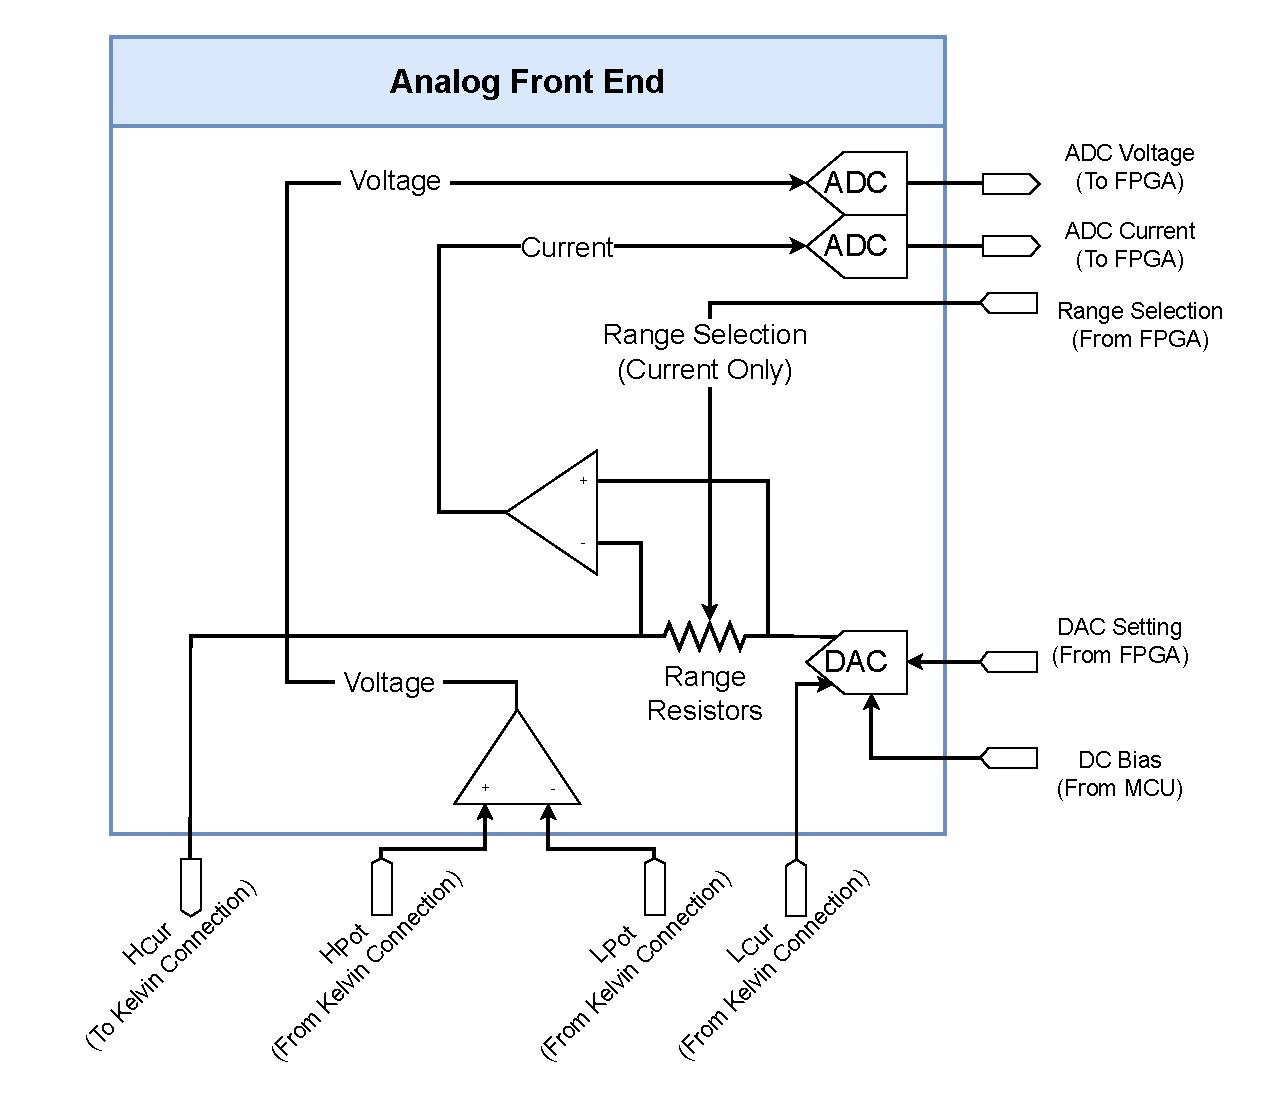
\includegraphics[clip, trim=18 0 18 0,width=0.70\textwidth]{Sections/6_SystemArchitecture/Figures/AnalogFrontEnd.pdf}
    \caption{The analog front end module. The DAC is generating the test signal for the DUT through the $H_{CUR}$, $L_{CUR}$ Kelvin Connections, while the two ADC's are sampling the DUT voltage through the $H_{pot}$ and $L_{pot}$ connections. The DUT current is sampled through a range resistor. All the control signal for the ADC and DAC come from the sample control module (marked as FPGA). The samples are stored in the sample control module. The  }
    \label{fig_6_1_AnalogFrontEnd}
\end{figure}

A DAC will generate the test signals for the DUT and two ADC's will sample the resulting current and voltage waveforms. The control signals for the DAC and the ADC's will come from the Sample Control Module. The DAC will drive the DUT through a programmable gain amplifier, allowing for different test voltages. This also has the benefit of allowign the DAC to run at a constant full-scale output, improving the signal to noise ratio. 

In much the same way, a Programable Gain Amplifier, PGA, is placed in front of each ADC, such that smaller voltages can be amplified, improving the signal to noise ratio of the analog to digital conversion. This also alows the design to better use the full dynamic range of both ADC's. The DAC \textit{side} of the analog front end will have a system to DC bias to the DUT as well, this means the DUT will see a sum of the test signal and DC bias voltage. The DC bias function is supplied by the Microprocessor module and will be described in section \refq{sec:MainProcessor}.

There are two ADC's in the module. ADC2 will acquire, and sample, the DUT current through a MUX'ed set of range resistors. A \textit{low} value of range resistor may be chosen if the DUT's impedance is low, and vice versa. The choice of range resistor will be decided by the sample control module, which will be described in section \refq{sec:Sample Control}. The sample control module will be controlling the choice of range resistor and the gain settings for the DAC's programmable amplifier. ADC1 will acquire, and sample, the voltage across the DUT. Both ADC1 and ADC2 will sample the current and voltage waveforms at the same time. The timing of this will be critical and is controlled by the sample control module.

The DAC and ADC's will have reconstruction and anti-aliasing filters. These are not shown on the block diagram but are assumed to be there.

The analog front end must interface with the Kelvin Connection, Sample Control and Main Processor modules, so their interfaces must be well defined. This will be shown in this section along with the modules specifications.


\subsection{Analog Front End Specifications} \label{subsec:AnalogFrontEndSpec}

\begin{table}[H]
    \begin{tabular}{|m{3.5em}|m{30em}|}
    \hline
      \textbf{ID} &   \textbf{Description}   \\ \hline
      §6.1.1 & Must be capable of sampling current and voltage at exactly the same time. \\ \hline
      §6.1.2 & The Acquisition time of sampled voltage must be less than \SIQ{50}{\nano\second}. \\ \hline
      §6.1.3 & The Acquisition time of sampled current must be less than \SIQ{50}{\nano\second}. \\ \hline
      §6.1.4 & The voltage measurement accuracy must be less \nl than$^1$ TBD. \\ \hline
      §6.1.5 & The current measurement accuracy must be less \nl than$^2$ TBD\\  \hline
      §6.1.6 & Jitter must not influence the phase of the measured voltage by more than $A_\theta(f_m, Z_m)/2$. \\ \hline
      §6.1.7 & Jitter must not influence the phase of the measured current by more than $A_\theta(f_m, Z_m)/2$.\\  \hline
      §6.1.8 & The bandwidth of the voltage measurement must be greater than \SIQ{1}{\mega\hertz}. \\ \hline
      §6.1.9 & The bandwidth of the current measurement must be greater than \SIQ{1}{\mega\hertz}.\\  \hline
      §6.1.10 & The bandwidth of current and voltage measurements must be matched to within \SIQ{0.1}{\decibel}.\\  \hline
      §6.1.11 & The bandwidth of the DAC must be greater than \SIQ{1}{\mega\hertz}. \\\hline
      §6.1.12 & The DAC must be capable of generating \SIQ{5}{\volt}$_{PP}$. \\ \hline
      §6.1.13 & The DAC must at least have a resolution of 10 bits. \\ \hline
      §6.1.14 & The DAC must be capable of supplying more than \SIQ{100}{\milli\ampere}$_{PP}$. \\ \hline
      §6.1.15 & The sample rate of the DAC must be greater than \SIQ{10}{\mega\hertz}.\\ \hline
      §6.1.16 & The analog front end must be capable of measuring currents from \SIQ{50}{\nano\ampere} to \SIQ{100}{\milli\ampere}. \\ \hline
    \end{tabular}
    \caption*{
      \raggedright
      $\mathbf{^1}$ Impedance fit refers to the model used to represent the impedance, see section \refq{subsec:SeriesToParallel}.\\
      $\mathbf{^2}$ The accuracy of the measured impedance magnitude, see section \ref{sec:ModulusArgumentAccuracy}. \\
    }
    \caption{Table to test captions and labels.}
    \label{tab:6_1_1ANFESpec}
  \end{table}
\subsection{Analog Front End Interface} \label{subsec:AnalogFrontEndInterface}
This section will define the interface between the Analog Front End and all other modules that can communicate with this module. The interface can be seen in table 
\ref{tab:6_1_2ANFEInterface}. In this talbe, ANFE refers to Analog Front End, PGA refers to Programable Amplifier and KC refers to Kelvin Connection.

\begin{table}[H]
    \begin{tabular}{|m{3.5em}|m{12.5em}|m{5em}|m{12.5em}|}
    \hline
    \textbf{Pins} &   \textbf{Type} & \textbf{Level} & \textbf{Description}  \\ \hline
    0-1 & ADC CLK & \SIQ{2.5}{\volt} \nl LVCMOS & ADC1, ADC2 CLK input. \nl ANFE $\leftarrow$ FPGA. \\ \hline
    2-3 & ADC DATA & \SIQ{2.5}{\volt} \nl LVCMOS & ADC1, ADC2 DATA output. \nl ANFE $\rightarrow$ FPGA. \\ \hline 
    4 & ADC CNV & \SIQ{2.5}{\volt} \nl LVCMOS & ADC1, ADC2 Trigger. \nl ANFE $\leftarrow$ FPGA. \\
    \hline
    5-7 & PGA1 gain, 5 is lsb & \SIQ{3.3}{\volt} \nl LVTTL & Setting for voltage PGA. \nl ANFE $\leftarrow$ FPGA. \\ \hline
    8-10 & PGA2 gain, 8 is lsb & \SIQ{3.3}{\volt} \nl LVTTL & Setting for current PGA. \nl ANFE $\leftarrow$ FPGA. \\ \hline
    11-13 & Range, 11 is lsb & \SIQ{3.3}{\volt} \nl LVTTL & Range setting. \nl ANFE $\leftarrow$ FPGA. \\ \hline
    14-29 & DAC Data , 14 is lsb& \SIQ{3.3}{\volt} \nl LVTTL & Data for DAC. \nl ANFE $\leftarrow$ FPGA.\\ \hline
    30 & DAC CLK & \SIQ{3.3}{\volt} \nl LVTTL & CLK for DAC. \nl ANFE $\leftarrow$ FPGA. \\ \hline
    31 & $H_{Cur}$ of kelvin connection & TBD & Current output to KC. \nl ANFE $\rightarrow$ KC. \\ \hline
    32 & $H_{Pot}$ of kelvin connection & TBD & Postive sence wire. \nl ANFE $\leftarrow$ KC. \\ \hline
    33 & $L_{POT}$ of kelvin connection & TBD & Negative sence wire. \nl ANFE $\leftarrow$ KC. \\ \hline
    34 & $L_{Cur}$ of kelvin connection & TBD & Current return from KC. \nl ANFE $\leftarrow$ KC. \\ \hline
    35 & DC Bias level & \SIQ{0}{\volt} - \SIQ{20}{\volt} & DC voltage for bias. \nl ANFE $\leftarrow$ MCU. \\ \hline
    \end{tabular}
    \caption{Table of the connections to and from the Analog Front End.}
    \label{tab:6_1_2ANFEInterface}
  \end{table}


\subsection{Choice of ADCs and DAC} \label{subsec:ADC_DAC_Choice}
The System requirements specify that the best case scenario accuracy of impedance magnitude must be less than \SIQ{0.1}{\%}. Impedance will be calculated as voltage divided by current, with both voltage and current being sampled by their own ADC. Assuming a worst case scenario where the error of one ADC directly adds to that of the other, such that the total ADC error can be given as $E_{ADC1}+E_{ADC2} = E_{ADC}$, the total ADC error $E_{ADC}$ should be less than the required magnitude accuracy, such that each ADC should be accurate to \SIQ{0.05}{\%}.

To ensure that the ADCs are accurate it has been chosen to use two 16 bit ADCs, more specifically two LTC2311 \cite{ADC_LTC2311}. These are 16 bit analog to digital converters with a maximum sample rate of 5 Msps. These offer a guaranteed integral non-linearity (INL) of less than 8 lsb, i.e. less than \SIQ{0.0122}{\%}, resulting in a guaranteed maximum ADC error $E_{ADC}$ of less than \SIQ{0.0244}{\%}.

This error assumes that \SIQ{100}{\%} of the ADCs range is utilized, this is of course not always the case. To find the minimum range the ADCs can be used within, the 8 LSB non-linearity can be considered as the maximum allowed \SIQ{0.05}{\%} error. This can be seen in equation \ref{eq:6_1_3_ADC_range_error}. Here it is also shown that the ADCs can be used down to only \SIQ{24.4}{\%} of their range. This ensures that even if the ADCs full range is not used, the non-linearity at least should not add more error than tolerated.

\begin{equation}
\begin{split}
    \label{eq:6_1_3_ADC_range_error}
    n_{range} &= \frac{INL}{Error_{MAX}} \cdot 100 \\
    \Rightarrow n_{range} &= \frac{8}{0.05} \cdot 100 \\
    \Rightarrow n_{range} & = 16000 \Rightarrow \frac{16000}{65535}\cdot 100 = \SIQ{24.4}{\%}
\end{split}
\end{equation}

Likewise a 16 bit DAC have been chosen, LTC1668 \cite{DAC_LTC1668}. This DAC is capable of 50 Msps, ensuring good spectral purity even at \SIQ{1}{\mega\hertz}.
\section{Main Processor} \label{sec:MainProcessor}
The stored samples inside the sample control module will be retrieved by the main processor module through a parallel bus. The main processor module will perform spectral analysis (DFT) on the samples and use these calculations to retrieve the magnitude and phase of the impedance. The module will then calculate all the derived quantities described in section \refq{subsec:DerivedQuantities} and transmit them to the UI module. The main processor module is shown on figure \refq{fig_6_4_MainprocessorModule}.

\begin{figure}[H]
    \centering
    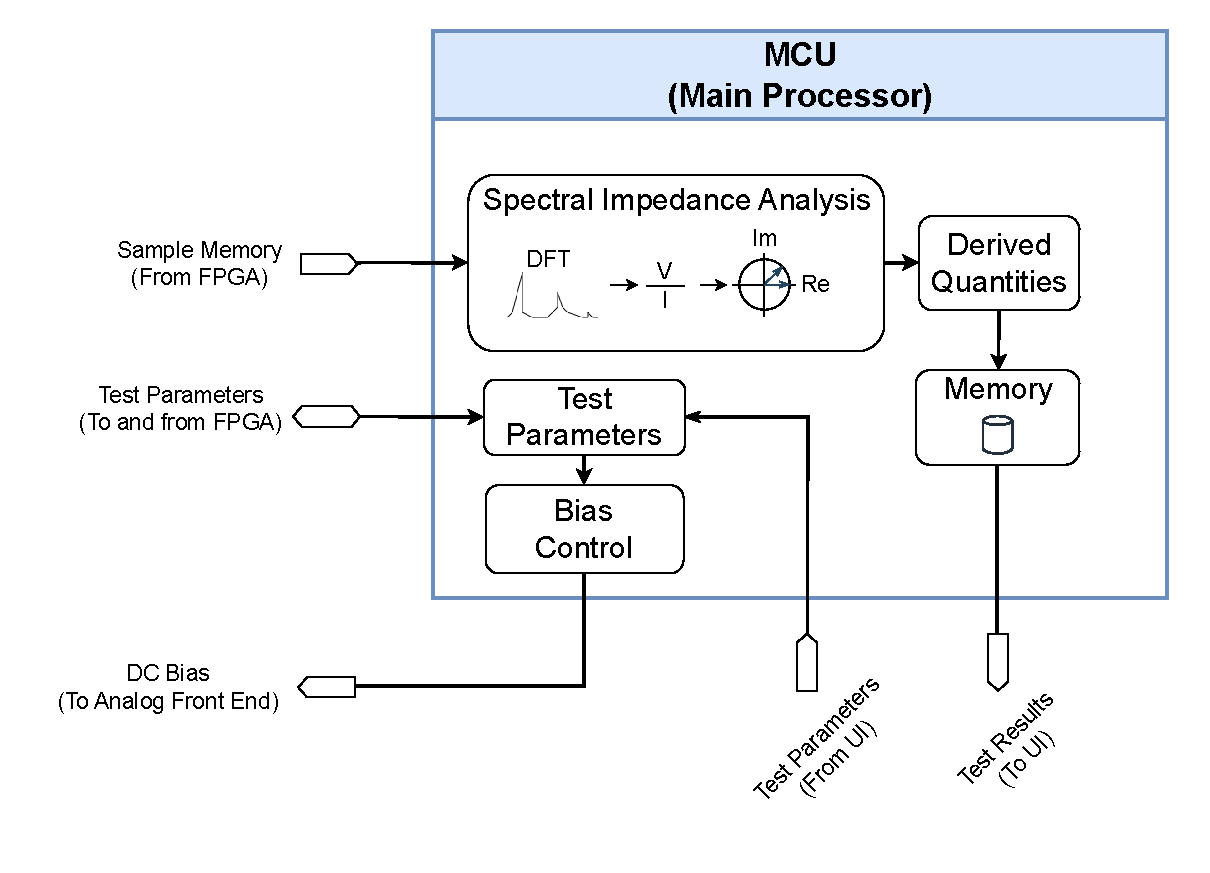
\includegraphics[clip, trim=18 0 18 0,width=0.70\textwidth]{Sections/6_SystemArchitecture/Figures/MCU.pdf}
    \caption{The main processor module takes the samples from the sample control modules memory and analyzes the samples in order to calculate the derived quantities and transmit them to the user interface module.}
    \label{fig_6_4_MainprocessorModule}
\end{figure}

The main processor module will also generate the DC bias voltage that is used inside the analog front end in order to bias the DUT. The module will, along with the DC bias, transmit all the relevant test parameters to the FPGA. The test parameters can be parameters such as test frequency, DC bias level, sample size and so on. The user can choose many of these test parameters in the UI module and the main processor module will take these choices and send them to the relevant modules.

\subsection{Main Processor Specifications} \label{subsec:MainProcessorSpecifications}

\subsection{Main Processor Interface} \label{subsec:MainProcessorInterface}
This section will define the interface between the Microcontroller module and all other modules that can communicate with this module. The interface can be seen in table 
\ref{tab:6_4_2MCUInterface}. In this talbe, ANFE refers to Analog Front End. A pin map of the connectios between the MCU and Sampel Control modules can be seen in appendix \ref{App:PinMap_MCU_FPGA}.
\begin{table}[H]
    \begin{tabular}{|m{3.5em}|m{12.5em}|m{5em}|m{12.5em}|}
    \hline
    \textbf{Pins} &   \textbf{Type} & \textbf{Level} & \textbf{Description}  \\ \hline
    0-15 & Parallel data bus IO, 0 is lsb & \SIQ{3.3}{\volt} \nl LVTTL & Data and address bus for MCU and FPGA. \nl FPGA $\leftarrow \rightarrow$ MCU. \\ \hline
    16 & Parallel data bus R/W & \SIQ{3.3}{\volt} \nl LVTTL & Read or write data to/from the FPGA. \nl FPGA $\leftarrow$ MCU. \\ \hline
    17 & Parallel data bus CLK & \SIQ{3.3}{\volt} \nl LVTTL & Clock for the data bus. \nl FPGA $\leftarrow$ MCU. \\ \hline
    18 & DC Bias Voltage for DAC & \SIQ{0}{\volt} - \SIQ{20}{\volt} & DC bias output \nl ANFE $\leftarrow$ MCU. \\ \hline
    19 & DC Bias On/Off & \SIQ{3.3}{\volt} \nl LVTTL & On/Off switch for DC bias. \\ \hline
    20-21 & UART RX/TX & \SIQ{3.3}{\volt} \nl LVTTL & MCU $\leftarrow \rightarrow$ UI \SIQ{115.2}{\kilo\bit} \\ \hline
    \end{tabular}
    \caption{Table to test captions and labels.}
    \label{tab:6_4_2MCUInterface}
\end{table}


  
\subsection{Choice of processor} \label{subsec:MainProcessorChoice}

Based on choice of architecture and desired functions along with the specifications listed in sections \refq{subsec:MainProcessorSpecifications} and \refq{subsec:MainProcessorInterface}, it is clear that the microprocessor will be doing a significant amount of floating point operations, so the microprocessor should have an FPU and a \textit{high} clock frequency to minimize compute times. It should also have a DAC to generate a DC bias voltage for the analog front. It should have a UART to communicate with a user interface and it should have a significant amount of RAM to store the impedance, phase, frequency and derived quantities. 

The microcontroller in the project will be an STM32F446RE\cite{ST_STM32F446RE} embedded on an ST NUCLEO-F446RE\cite{ST_NUCLEOF446RE} development board. The STM32 platform is convenient for development purposes as the underlying ST hardware abstraction layer (HAL) drivers enables the team to quickly swap to a different microcontroller in case more functions are required, such as additional RAM, SPI's, GPIO's, high clock rates and so on. The STM32F446RE was chosen as it was the most capable STM32 development board available to the project team at the time. It is running at a maximum core clock frequency of \SIQ{180}{\mega\hertz}. It directly supports floating point operations, it has a DAC and plenty of I/O to connect with the other modules in the project and it is easily upgradeable if it proves insufficient later in the project.

As the microprocessor will need to communicate with the sample control module, some consideration and tests were conducted  to evaluate how quickly it can set and clear it's I/O pins, swap input states, perform bitwise operations and perform floating point operations. This can all be seen in appendix \refq{App:MicrocontrollerConsiderations}.

Specification §6.4.6 states that the microprocessor should be able to store 10000 impedance magnitude values, phase angle values and frequency values. The maximum frequency value is \SIQ{1}{\mega\hertz}. These are all 32bit wide variables, so the memory required is $Mem = 3\cdot 10E3 \cdot 32 = 960 kbit$ for storing these values. The STM32F446RE has \SIQ{128}{\kilo\bit} available SRAM, so additional external memory is required, this will be important in the system design.

Using the STM32F446 to directly control the sampling of the ADC's was considered, so the jitter of an output pin of the microcontroller was tested, this can also be seen in appendix \refq{App:MicrocontrollerConsiderations} on microcontroller considerations. The jitter caused by the microcontroller would cause a phase error of about 5\degree at \SIQ{1}{\mega\hertz} and this is significantly more than the system requirements specified in section \refq{ch:SystemRequirements} allow, so the microprocessor is not suitable for controlling the acquisition signals of the two ADC's as they must be triggered at the same time and with the same interval. The problem is made worse by the fact that the sampling will be done over a longer period of time.



\section{Sample Control} \label{sec:Sample Control}

\subsection{Sample Control Specifications} \label{subsec:SampleControlSpec}

\subsection{Sample Control Interface} \label{subsec:SampleControlInterface}
This section will define the interface between the Sample Control module and all other modules that can communicate with this module. The interface can be seen in table 
\ref{tab:6_3_2FPGAInterface}. In this talbe, ANFE refers to Analog Front End, PGA refers to Programable Amplifier.
\begin{table}[H]
    \begin{tabular}{|m{3.5em}|m{12.5em}|m{5em}|m{12.5em}|}
    \hline
      \textbf{Pins} &   \textbf{Type} & \textbf{Level} & \textbf{Description}  \\ \hline
      0-15 & Parallel data bus IO, 0 is lsb & \SIQ{3.3}{\volt} \nl LVTTL & Data and address bus for MCU and FPGA. \nl FPGA $\leftarrow \rightarrow$ MCU. \\ \hline
      16 & Parallel data bus R/W & \SIQ{3.3}{\volt} \nl LVTTL & Read or write data to/from the FPGA. \nl FPGA $\leftarrow$ MCU. \\ \hline
      17 & Parallel data bus CLK & \SIQ{3.3}{\volt} \nl LVTTL & Clock for the data bus. \nl FPGA $\leftarrow$ MCU. \\ \hline
      18-19 & ADC CLK & \SIQ{2.5}{\volt} \nl LVCMOS & ADC1, ADC2 CLK input. \nl ANFE $\leftarrow$ FPGA. \\ \hline
      20-21 & ADC DATA & \SIQ{2.5}{\volt} \nl LVCMOS & ADC1, ADC2 DATA output. \nl ANFE $\rightarrow$ FPGA. \\ \hline 
      22 & ADC CNV & \SIQ{2.5}{\volt} \nl LVCMOS & ADC1, ADC2 Trigger. \nl ANFE $\leftarrow$ FPGA. \\
      \hline
      23-25 & PGA1 gain, 23 is lsb & \SIQ{3.3}{\volt} \nl LVTTL & Setting for voltage PGA. \nl ANFE $\leftarrow$ FPGA. \\ \hline
      26-28 & PGA2 gain, 8 is lsb & \SIQ{3.3}{\volt} \nl LVTTL & Setting for current PGA. \nl ANFE $\leftarrow$ FPGA. \\ \hline
      29-31 & Range, 11 is lsb & \SIQ{3.3}{\volt} \nl LVTTL & Range setting. \nl ANFE $\leftarrow$ FPGA. \\ \hline
      32-47 & DAC Data , 14 is lsb& \SIQ{3.3}{\volt} \nl LVTTL & Data for DAC. \nl ANFE $\leftarrow$ FPGA.\\ \hline
      48 & DAC CLK & \SIQ{3.3}{\volt} \nl LVTTL & CLK for DAC. \nl ANFE $\leftarrow$ FPGA. \\ \hline
    \end{tabular}
    \caption{Table to test captions and labels.}
    \label{tab:6_3_2FPGAInterface}
  \end{table}
\subsection{Choosing an FPGA} \label{subsec:ChoosingAnFPGA}

Based on the jitter issues with the STM32F446 microprocessor mentionen in subsection \refq{subsec:MainProcessorChoice} and appendix \refq{App:MicrocontrollerConsiderations} it was decided to let an FPGA control all the sampling and timing of the ADC's and DACs in the analog front end. FPGA's are typically used for this exact purpose in other instruments. The only consideration for the choice of FPGA in this project is that it should have sufficient GPIO pins, it should produce \textit{low} jitter output signals and it should have sufficient memory to store the samples.

It can be seen in the interface specification \refq{subsec:SampleControlInterface} that the FPGA should have 46 GPIO pins to connect with the Main Processor module and Analog Front End module. The FPGA (module) should have \SIQ{320}{\kilo\bit} memory for storing the 10000 16 bit values of current and voltage samples.

The Digilent CMOD A7\cite{CMOD_A7_AT35T} with an Artix 7 35T-236 AMD-Xilinx FPGA\cite{ARTIX7} will be used for this project as the team members have prior experience working with this FPGA. The FPGA has 56 GPIO pins and comes with \SIQ{512}{\kilo\byte} external SRAM which is more than sufficient for this project. The FPGA also has very low jitter and the project team was not able to actually measure it with the instruments that are available, so, it is suitable for controlling the sampling signals for the ADCs.





\section{User Interface} \label{sec:UserInterface}
The user interface module, shown on figure \refq{fig_6_5_UserInterface}, is a touchscreen that the user can use to set the test parameters for the DUT. The screen will display the test results to the user in whichever format the user has choser, either numerically or with a graph.

\begin{figure}[H]
    \centering
    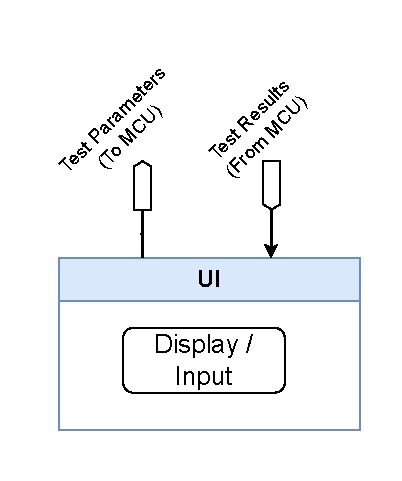
\includegraphics[clip, trim=18 0 18 0,width=0.40\textwidth]{Sections/6_SystemArchitecture/Figures/UI.pdf}
    \caption{The user interface is a touchscreen. The user can set the test parameters for the DUT and the display can show the results.}
    \label{fig_6_5_UserInterface}
\end{figure}

The \textit{user interface} module is also a USB device that the user can use to retrieve test results from the instrument. It is envisioned that the user can start a transfer from the impedance analyzer and the instrument will then proceed to dump all the test results in a string of comma separated values over the serial connection. It will be up to the user to \textit{listen in} and log the results from a serial monitor such as puTTY, or similar.

\subsection{User Interface Specifications} \label{subsec:UserInterfaceSpecifications}

\subsection{User Interface} \label{subsec:UserInterface}
This section will present the connections interface between the UI and the MCU.
\begin{table}[H]
    \begin{tabular}{|m{3.5em}|m{12.5em}|m{5em}|m{12.5em}|}
    \hline
    \textbf{Pins} &   \textbf{Type} & \textbf{Level} & \textbf{Description}  \\ \hline
    0-1 & UART RX/TX & \SIQ{3.3}{\volt} \nl LVTTL & MCU $\leftarrow \rightarrow$ UI \SIQ{115.2}{\kilo\bit} \\ \hline
    \end{tabular}
    \caption{The interface for the main processor and UI modules is just a UART connection.}
    \label{tab:6_5_2UIInterface}
\end{table}

%System design
\chapter{Module Design} \label{ch:SystemDesign}



\section{Analog Front End Module} \label{sec:AnalogFrontEndModule}
\section{Sample Control Module} \label{sec:SampleControl}
The Sample Control module is the module responsible for generating the necessary inputs for a DAC that will generate the DUT input test signals and for controlling the ADCs that are sampling the resulting DUT voltage and current waveforms simultaneously. The module will take the samples from the ADCs and store them in external memory. The external memory can be accessed by the Main Processor module in order to retrieve and analyze the samples. The Sample Control module will accept test parameters from the Main Processor and store them in internal registers, these internal registers are connected to the internal sample control logic and can be used to adjust the sampling parameters. The block diagram for the Sample Control module can be seen on figure \refq{fig:7_SampleControlBlock}.
\begin{figure}[H]
    \centering
    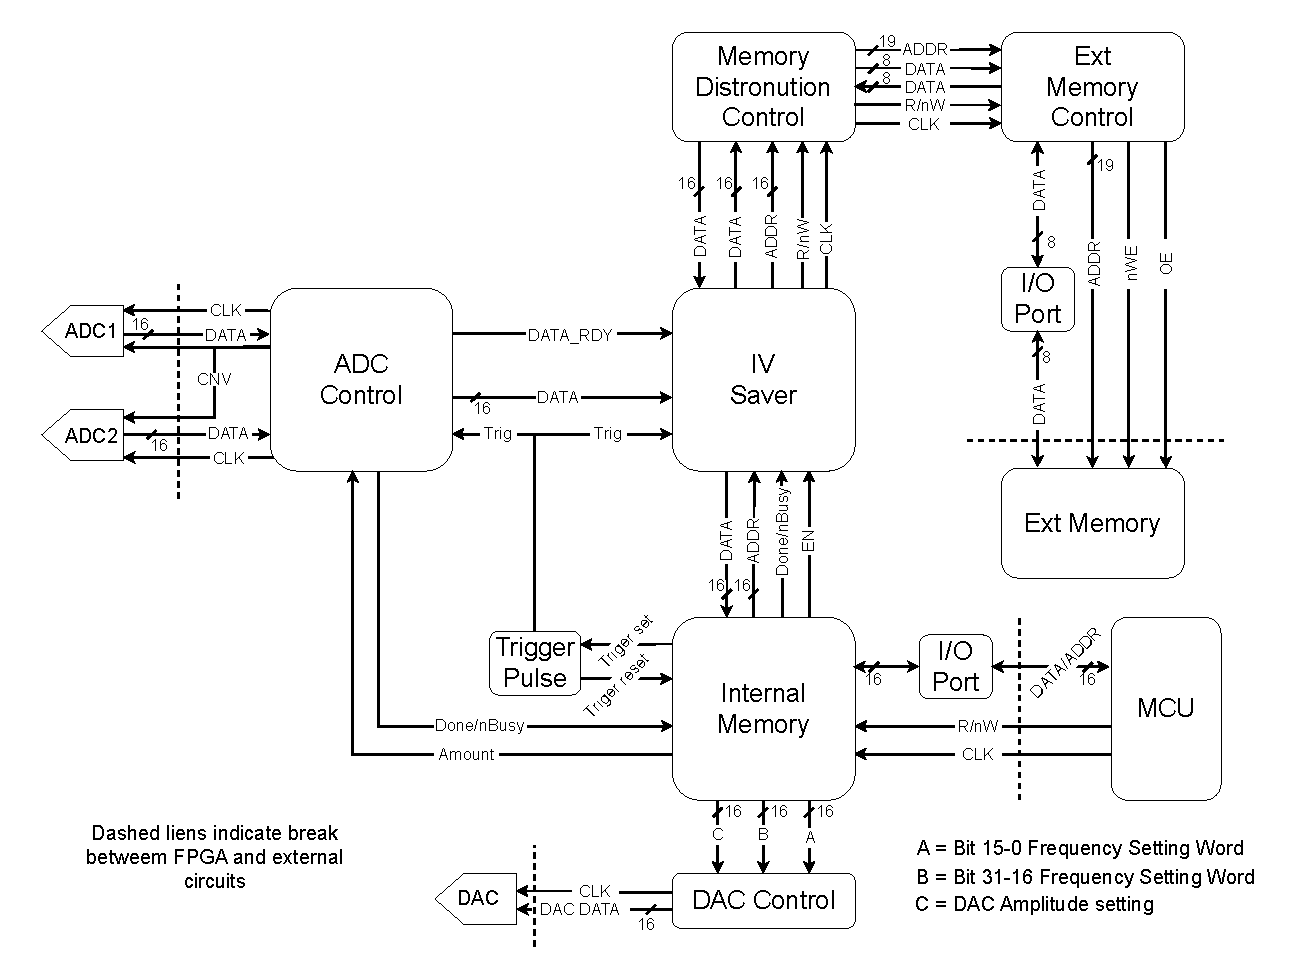
\includegraphics[clip, trim=0 0 0 0, width=1\textwidth]{Sections/7_SystemDesign/Figures/Sample_Control_Block.pdf}
    \caption{Block diagram of the internal logic blocks of the Sample Control Block.}
    \label{fig:7_SampleControlBlock}
\end{figure}

The block diagram on figure \refq{fig:7_SampleControlBlock} has a number of logic blocks. The MCU will connect to the Sample Control(SCM) module through a parallel communication bus and it can do writes, or reads, to a number of internal registers in the Internal Memory block, and use these registers to adjust test parameters such as test frequency, sample rate, sample size and it can start a sampling process. 

The DAC Control block is controlling the stimulus inputs for the external DAC that is generating the test signal going into the DUT. The frequency of this DAC can be set in a register in the internal memory. A sampling process will start when the MCU has set a 'trigger' flag in a register in the internal memory. This register connects to the ADC Resampler logic and this logic will generate the acquisition signals for the ADC Control block. The ADC Resamper will generate an acquisition pulse for every sample until it has reached the desired sample size. The ADC Control logic will control the timing of the two ADCs necessary to sample the DUT voltage and current. It will sample the ADCs every time it recieves and acquisition input from the ADC Resampler and send the samples to the Parallel To Series Converter logic.

The two ADCs are sampled at the same time, but the external memory can store just one sample at a time. The Parallel To Series logic will take the two samples and trigger the IV Saver, Memory Distribution and External Memory Control logic twice, one for each sample, in order to cause these other logic blocks to save the two samples.

The IV Saver is a MUX that controls the input/output path to the external memory. During a sampling process it will forward data to the external memory through the Memory Distribution Control block, and when no sampling process is active, it will allow the MCU to read from the external memory.

The IX MUX block is a MUX that is connected to an input pin that the MCU can control. Depending on the state of this pin the MCU can access the internal memory registers, or it can read from the external memory through the IV Saver logic.

All the logic blocks on figure \refq{fig:7_SampleControlBlock} will be described in detail in this section.
\subsection{Communication} \label{subsec:Communication}
The Main Processor and Sample Control modules need a communication interface in order to set control settings for the ADCs, DAC in the FPGA's internal registers and to retrieve stored ADC samples.The ADCs and DAC \todo{Vi mangler at redegøre for det her valg.} both have 16 bits of resolution and a 16 bit wide parallel bus between the FPGA and MCU will be used to transfer the data as shown on figure \refq{fig_7_2_1_CommBus}.

\begin{figure}[H]
    \centering
    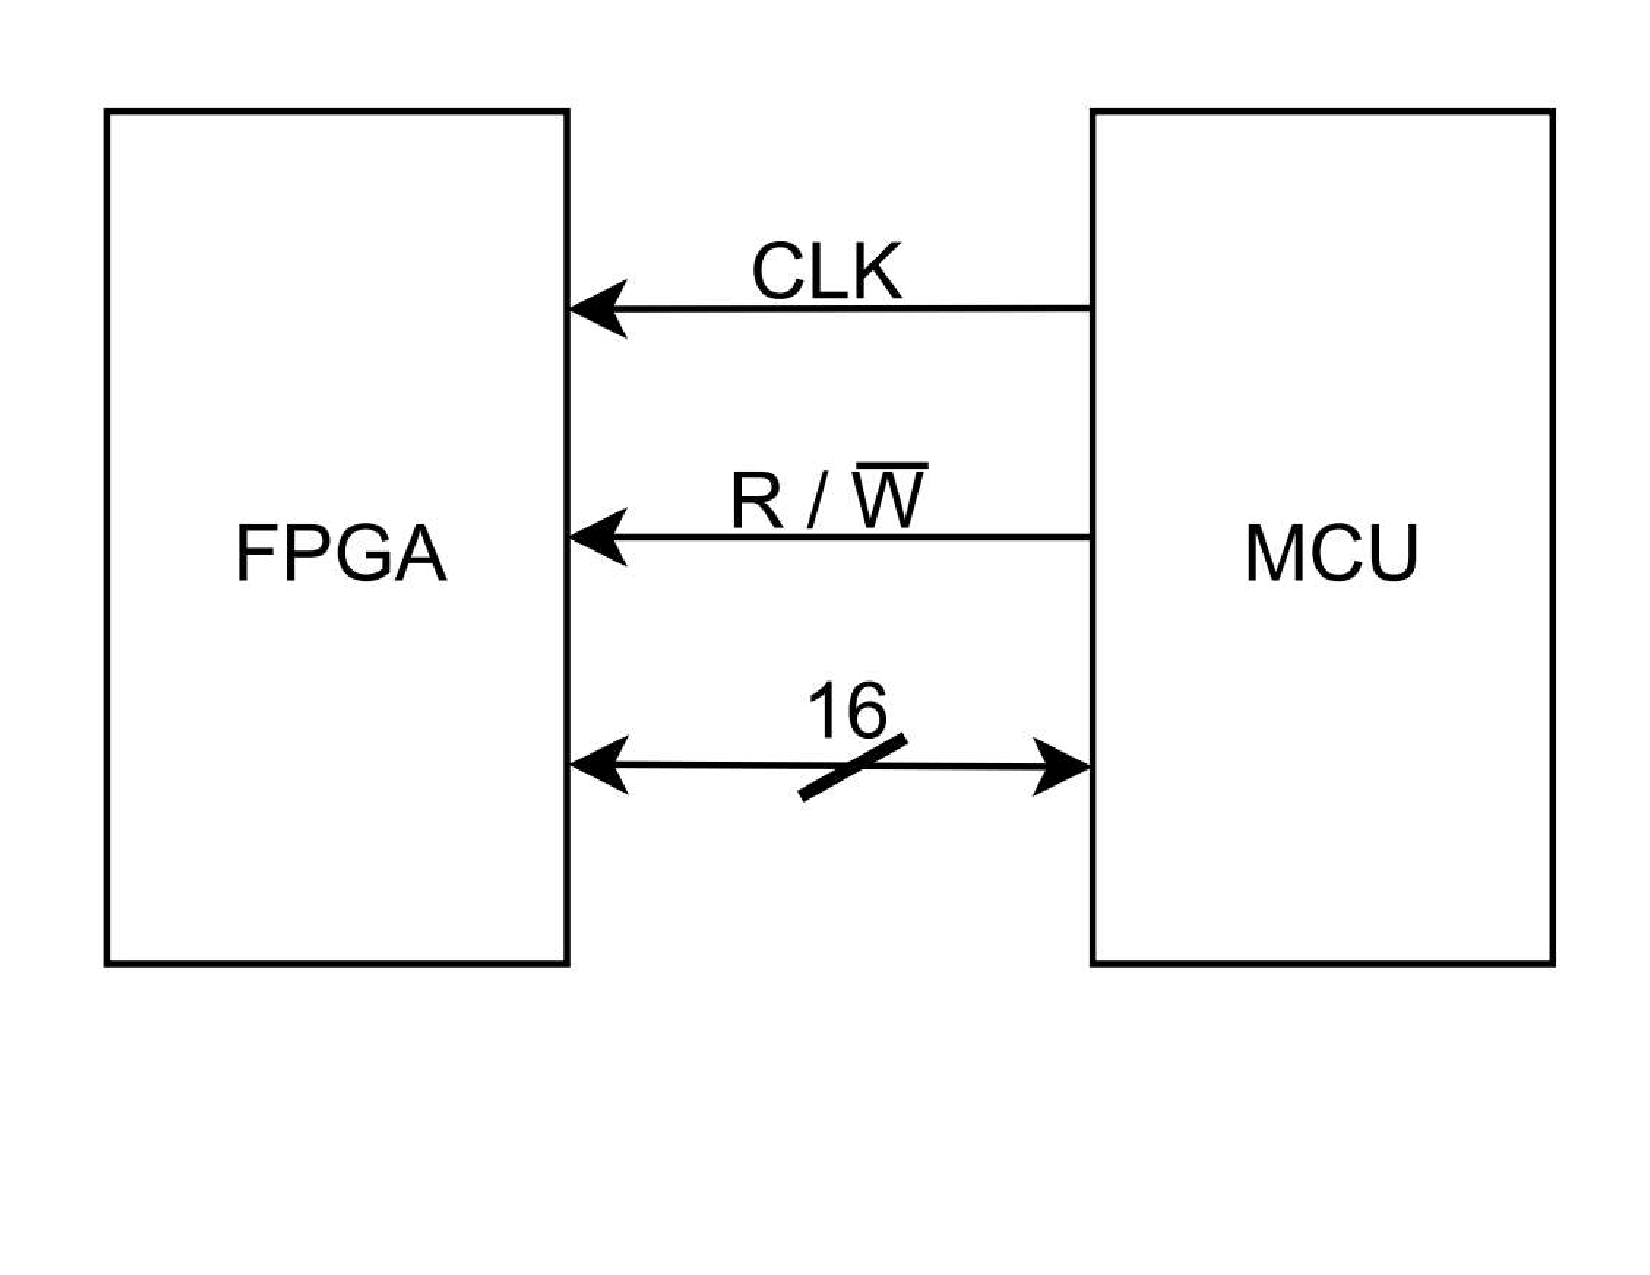
\includegraphics[clip, trim=0 100 0 0, width=0.5\textwidth]{Sections/7_SystemDesign/Figures/7_2_1_CommunicationBus.pdf}
    \caption{The communication bus connection the FPGA and microcontroller. It uses a 16 bit databus, a long with a CLK and a read/write control signal.}
    \label{fig_7_2_1_CommBus}
\end{figure}

The microcontroller is always going to be the master that has to initiate communication and the FPGA is always the slave. The microcontroller is controlling the read/write and CLK control signals necessary for the communication to work. The Read-write pin is, when  RW = '0', in write mode and in read mode when RW = '1'. Data is clocked in and out on the rising edges of the CLK. 

If the MCU wants to write some value into a register it must first CLK in an address into the FPGA before it can CLK in any data, as shown on figure \refq{fig_7_2_1_CommWrite}. 
\begin{figure}[H]
    \centering
    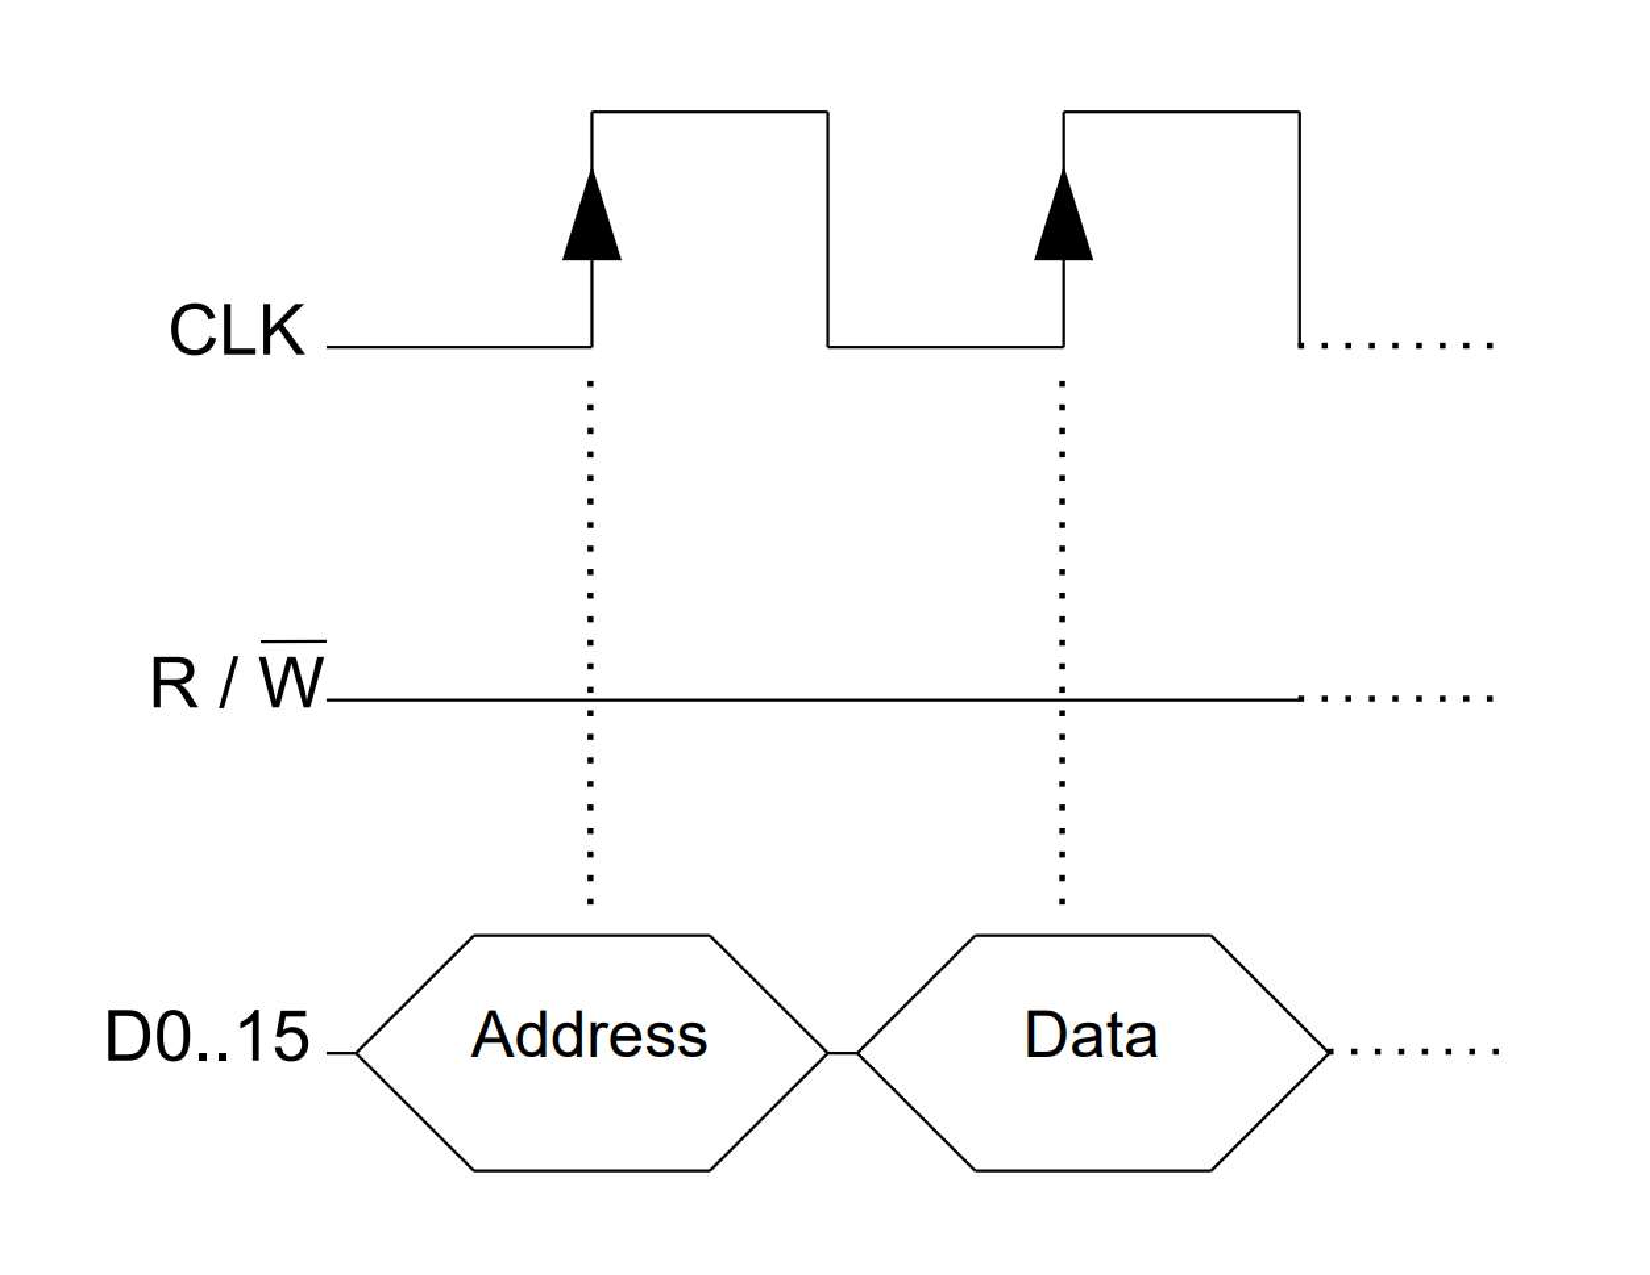
\includegraphics[clip, trim=0 50 0 0, width=0.5\textwidth]{Sections/7_SystemDesign/Figures/7_2_1_CommWrite.pdf}
    \caption{In order to write to the FPGA, the MCU must first set RW ='0' then set the 16 bit bus to the desired address and generate a single CLK pulse. The address is clocked into the FPGA on a rising edge. To write data into the address; the MCU sets 16 bit data on the bus and then generate a single clock pulse. Data is clocked into the FPGA on a rising edge.}
    \label{fig_7_2_1_CommWrite}
\end{figure}

Note how on figure \refq{fig_7_2_1_CommWrite} D0..D15 should have settled before the MCU tries to clock in any value. This will be ensured by design as the signals for the communication are generated sequentially in software on the MCU. They are not hardware controlled and there will be a minimum of \SIQ{35.8}{\nano\second} between D0..D15 and CLK as shown in appendix \refq{App:MicrocontrollerConsiderations} and significantly more if the MCU wants to read from the FPGA.

If the MCU wants to read from the FPGA it must first CLK in an address in the same way as for a write operation, then change it's D0..D15 output pins to input pins and set RW '1'. The following CLK will cause the FPGA to set the data unto the bus pins as shown on figure \refq{fig_7_2_1_CommRead}. \todo{placeholder billede}

\begin{figure}[H]
    \centering
    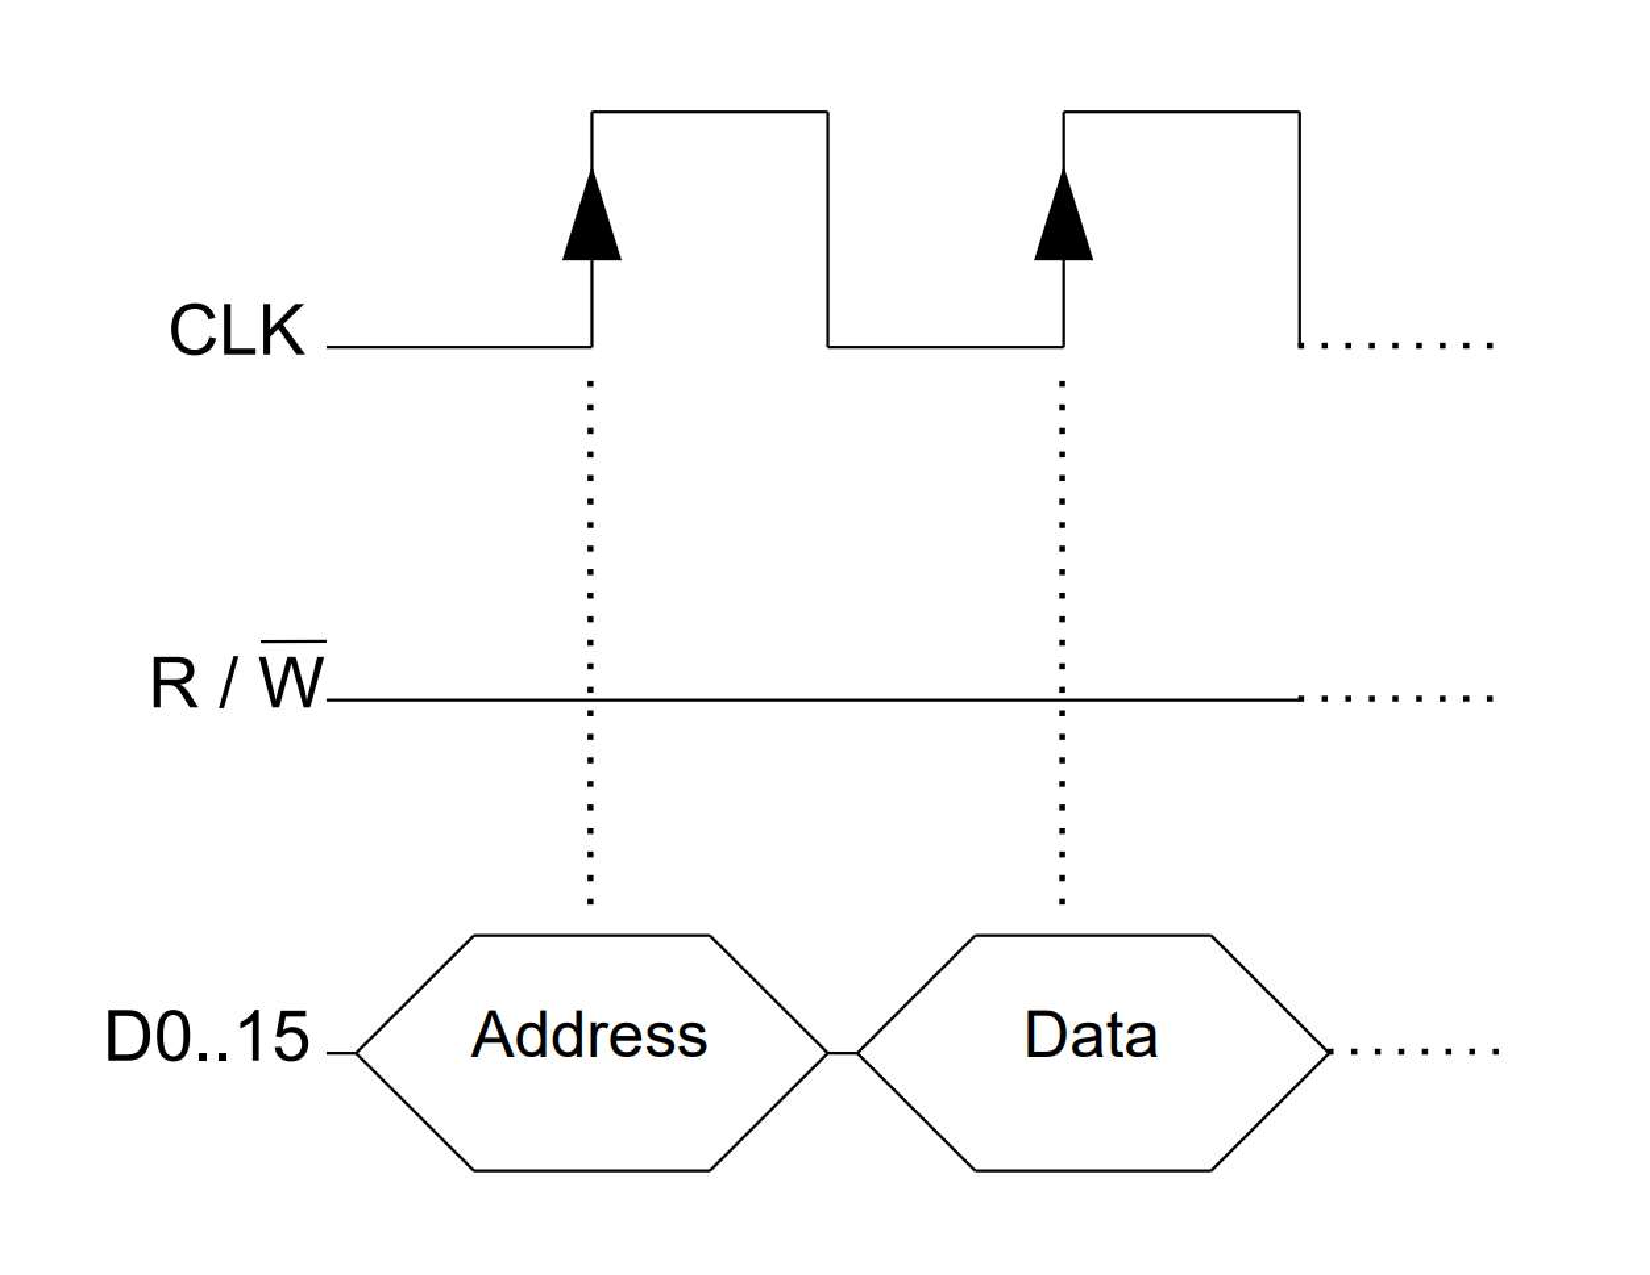
\includegraphics[clip, trim=0 50 0 0, width=0.5\textwidth]{Sections/7_SystemDesign/Figures/7_2_1_CommWrite.pdf}
    \caption{In order to read from the FPGA, the MCU must first set RW ='0' then set the 16 bit bus to the desired address and generate a single CLK pulse. The address is clocked into the FPGA on a rising edge. To read data from the address; the MCU sets RW = '1' and changes it's DB0..DB15 outputs to input. The FPGA clocks the data out on DB0..DB15 on the next rising edge.}
    \label{fig_7_2_1_CommRead}
\end{figure}

The FPGA is using tri-state buffers to function as both inputs and outputs. The Artix 7 FPGA development board is an expensive component and it was decided to let the FPGA use open-drain outputs in order to reduce the risk of both FPGA and MCU actively driving the data bus because of a mistake during development. The logic for this hardware can be seen on listing \refq{lst:7_2_1_CommPort}. 'TOPORT' is data from the internal RAM going to the I/O port and 'TORAM' is data from the I/O going to the RAM.

\lstinputlisting[language=C ,style = c,firstnumber=1, linerange=56-67, caption={VHDL code for the tri-state buffers}, label={lst:7_2_1_CommPort}]{Sections/7_SystemDesign/Code/comm_port.vhd}

The assignment of 'Z' to an 'inout' pin in line 5 will cause the output to enter a high impedance state when it has to produce a logic '1'. This can also be seen on the truth table for the communication port pins as shown on figure \refq{fig_7_2_1_TruthTable}.

\begin{figure}[H]
    \centering
    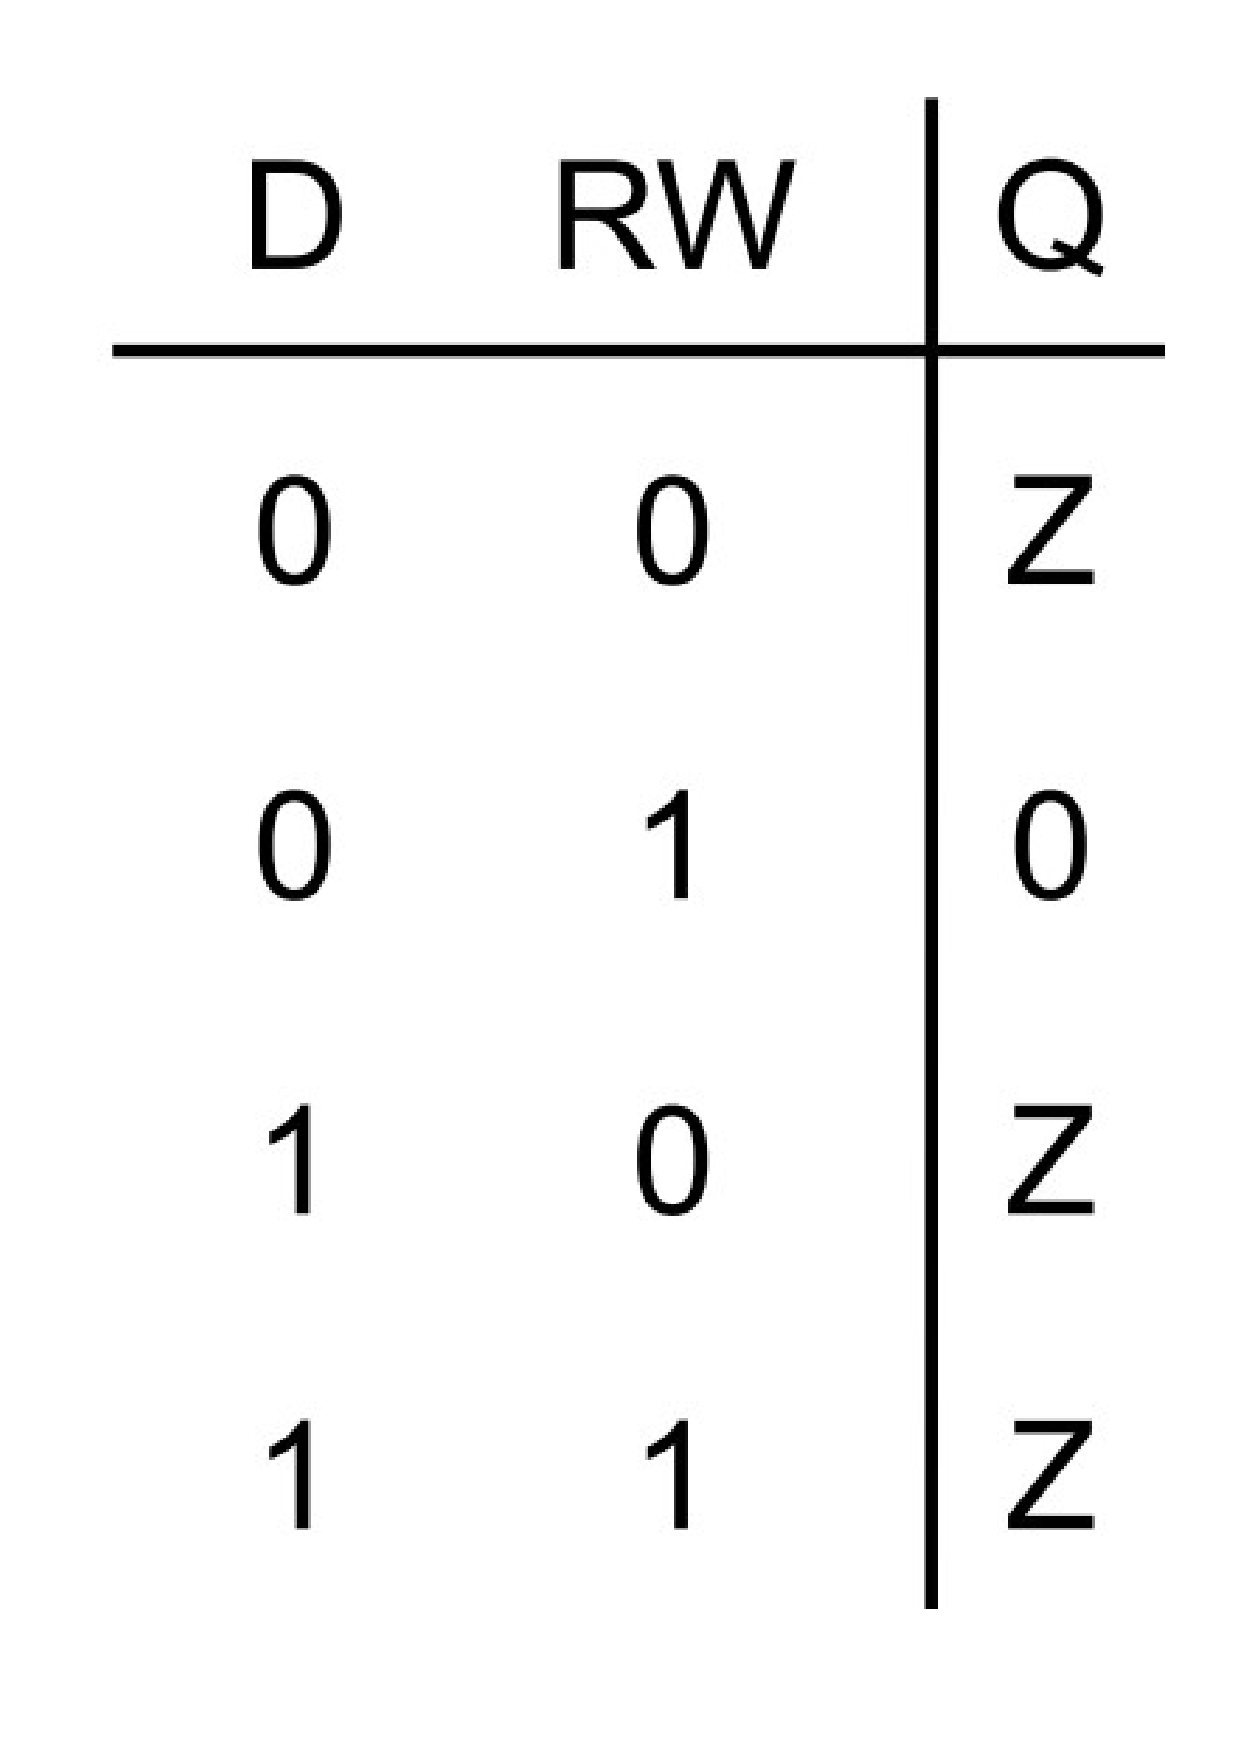
\includegraphics[clip, trim=0 50 0 0, width=0.2\textwidth]{Sections/7_SystemDesign/Figures/7_2_1_IOPortLogic.pdf}
    \caption{A truth table for the input/output port of the FPGA. RW = '0' always puts the port into a high impedance state and RW = '1' lets the port pull the I/O pin to '0'.}
    \label{fig_7_2_1_TruthTable}
\end{figure}

At first glance the I/O port logic on figure \refq{fig_7_2_1_TruthTable} may seem completely useless as it can't output a logic '1'. This is because the I/O pins will require external pull-up resistors in order to produce a '1' when RW = '1'. This will reduce the chance of both FPGA and MCU driving the databus at the same time. The only possible way of damaging the FPGA with the communication bus is if the MCU sets it's output high when RW = '1' and the FPGA sets a '0' as the FPGA pins are high impedance in any other case.

\subsubsection{Communication data rate} \label{subsubsec:CommunicationDatarate}

An estimate of the data rate from this databus can be made based on the findings in appendix \refq{App:MicrocontrollerConsiderations}. For consecutive read operations where the RW signal remains in 'write' mode, the datarate will be limited by the execution time of setting the register in the STM32F446RE. This is also described in appendix \refq{App:MicrocontrollerConsiderations}. From the appendix it takes $t_{clk} = 35.8$ns to toggle the pin by setting and clearing a register and a write to a single register will take $t_{rs} = 17.9$ns. This is useful for calculating the communication throughput.

Every write operation to the RAM requires a 16bit address and 16bit data and two toggles of the CLK. It can be seen in appendix \refq{App:PinMap_MCU_FPGA} on the pin map that the databus on the STM32F446Re is spread over two separate ports, so the MCU will have to write(and read) to two seperate registers in order to write to the FPGA. This is a limitation of the Nucleo development board being used, it would otherwise be possible to do this with a single port, and thus a single register transfer. The total amount of register writes for a single write operation will be as shown in eq \refq{eq:7_2_1_Write_ThroughPut}.

\begin{equation}\label{eq:7_2_1_Write_ThroughPut}
    n_{reg} = n_{clk} +  n_{address} + n_{write} = 4+2+2 = 8 
\end{equation}
It takes a total of 8 register writes to perform a single write operation to the FPGA as shown in equation \refq{eq:7_2_1_Write_ThroughPut}. 4 for toggling the CLK pin twice and 2 each for setting the address and data on the IO pins. Each register write takes \SIQ{17.9}{\nano\second} so the total execution times for a write operation is \SIQ{143.2}{\nano\second} as shown in eq\refq{eq:7_2_1_Write_ThroughPutTotalTime}.
\begin{equation}\label{eq:7_2_1_Write_ThroughPutTotalTime}
    t_{write} = t_{rs} \cdot n_{reg} = 17.9e-9 \cdot 8 =  143.2e-9
\end{equation}
It takes \SIQ{143.2}{\nano\second} for the MCU to perform a write operation. The total throughput on the bus in write mode will be about \SIQ{7}{\mega\bit} as shown in equation \refq{eq:7_2_1_Write_ThroughPut}.

\begin{equation}\label{eq:7_2_1_Write_ThroughPut}
    R_{write} = \frac{1}{t_{write}} = 6.949e6 
\end{equation}
The throughput on the bus is about \SIQ{7}{\mega\bit} in write mode. A significant amount of the throughput is used on protocol overhead as half the transmissions are addresses. The protocol efficiency, $\eta_{p}$, is 

\subsection{Memory} \label{subsec:Memory}

\section{DAC Control} \label{subsec:DAC_CONTROL} 
Section \refq{ch:SysArchitecture} shows that the the Sample Controller is responsible for controlling the DAC such that a stable sine wave is generated. The logic responsible for this will be described in this section. The specific section of the Sample Controller that handles the DAC logic is referred to as the DAC Control. A block diagram of the DAC Control can be seen on figure \refq{fig:7_2_3_DAC_CONTROL}.

\begin{figure}[H]
    \centering
    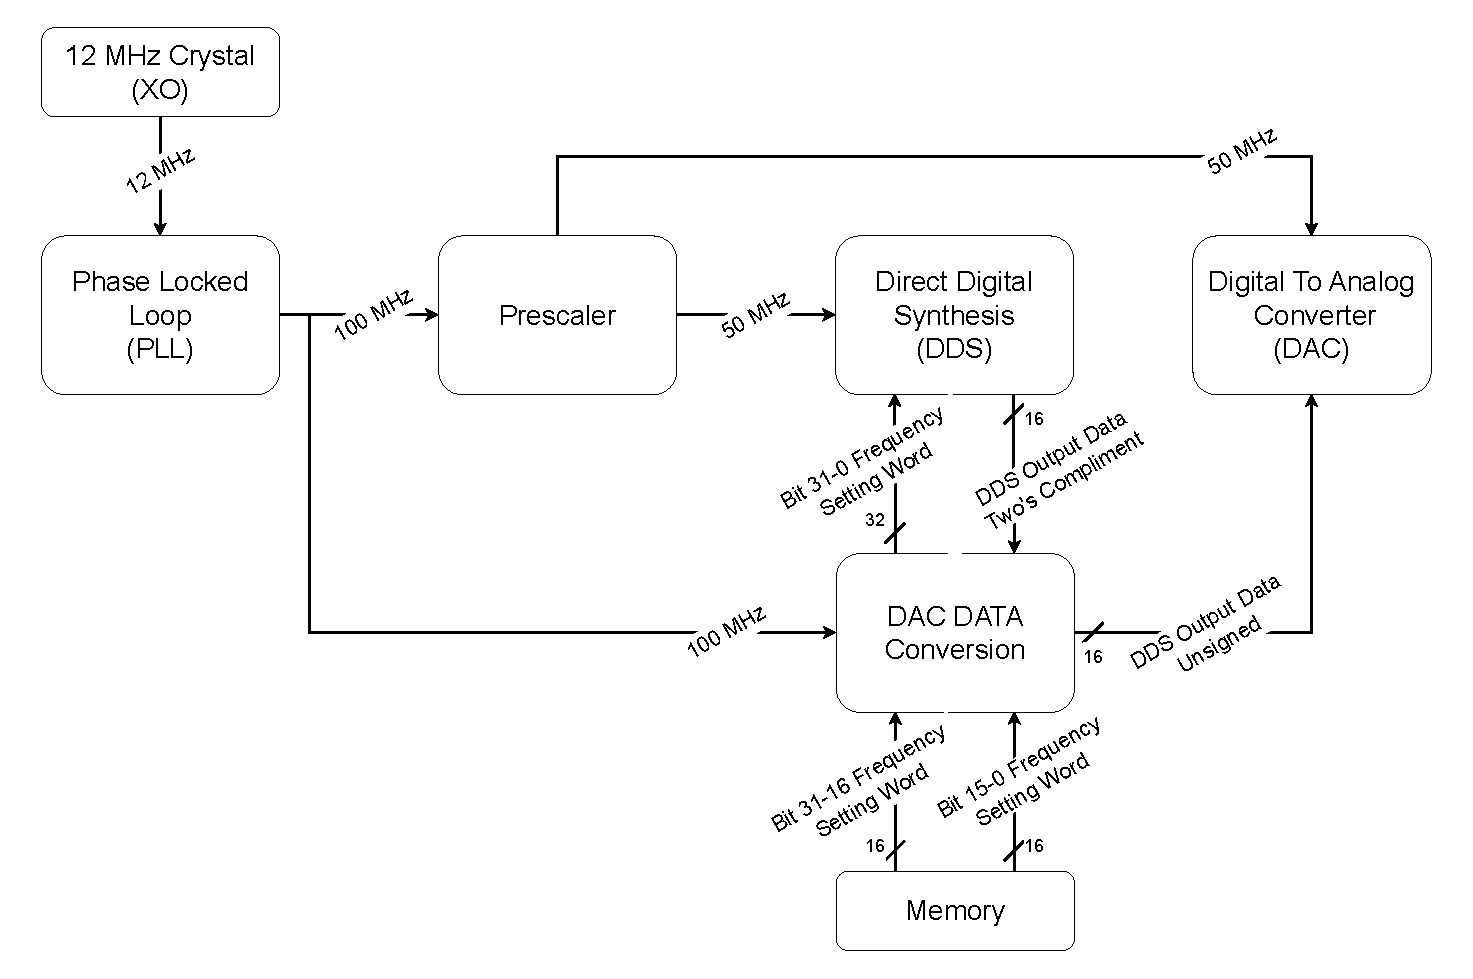
\includegraphics[clip, trim=0 0 0 0, width=1\textwidth]{Sections/7_SystemDesign/Figures/7_2_3_DAC_CONTROL.pdf}
    \caption{Block diagram of the DAC Control logic, the DAC is on the Analog Front End, it is shown here for completeness.}
    \label{fig:7_2_3_DAC_CONTROL}
\end{figure}

There are numerous of ways to generate sine waves, for this project a digital implementation has been favored due to the precise resolution that it offers. Requirement §1 from section \refq{ch:SystemRequirements} states that the frequency resolution must be at least \SIQ{1}{\hertz}. To achieve this, a Direct Digital Synthesis (DDS) principle has been implemented. This essentially allows for a frequency resolution that is the DAC update rate divided by the length of the frequency setting word \cite{Fundamentals_DDS}. With a 32 bit wide frequency setting word, as specified by requirement §6.3.13 in section \refq{subsec:SampleControlSpec}, the resulting frequency resolution would be $f_{res} = \frac{DAC_{CLK}}{2^{32}}$.

The used DAC is an LTC1668, capable of an update rate of \SIQ{50}{\mega\hertz}, it has however been decided to use \SIQ{20}{\mega\hertz} as \SIQ{50}{\mega\hertz} square waves are rather difficult to handle on development boards. This essentially allows for a frequency resolution of \SIQ{4.6566}{\milli\hertz}, see equation \refq{eq:7_2_3_resolution}, assuming an update rate of \SIQ{20}{\mega\hertz}.

\begin{equation}
    \label{eq:7_2_3_resolution}
    f_{res} = \frac{\SIQ{20}{\mega\hertz}}{2^{32}} \Rightarrow \SIQ{4.6566}{\milli\hertz}. 
\end{equation}

Xilinx offers a complete "drag and drop" DDS block. The project team has settled on using this as it supports DAC resolutions of up to 26 bits and frequency setting words up to 48 bits, essentially making it ideal for the required DAC Control block. The principle of Direct Digital Synthesis will not be explained in this document, as it is not part of the scope of the project.

The DDS block is configured to take in a 32 bit wide frequency setting word, a \SIQ{20}{\mega\hertz} clock, and a frequency update signal. The output of the DDS block is configured for a 16 bit wide sine approximation as two's compliment.

All other blocks than the DDS shown in figure \refq{fig:7_2_3_DAC_CONTROL} are essentially there to "support" the DDS block. A \SIQ{20}{\mega\hertz} clock is generated via a Phase Locked Loop (PLL) and a prescaler. The PLL outputs a \SIQ{200}{\mega\hertz} signal that is divided by ten and fed to the DDS block. The prescaler will also generate a \SIQ{20}{\mega\hertz} pulse train that is delayed from the DDS clock signal. This delayed pulse train is used to update the DAC and to detect if a new frequency setting word is present. The PLL is an integrated solution from Xilinx, much like the DDS block, and as such it will not be explained further.

The 16 bit wide output data of the DDS contains an approximated full-scale sine wave in two's compliment. The DAC however requires unsigned values as an input, and thus the DDS output data must be converted to a 16 bit wide unsigned bus. Furthermore the memory holds data in 16 bit registers, meaning that the 32 bit frequency setting word must be two registers that are concatenated. The DAC DATA Conversion block handles this concatenation and conversion from two's compliment to unsigned.

\subsection*{DDS and DAC Prescaler}
The clock for the DDS and DAC are both derived from the \SIQ{200}{\mega\hertz} master clock. This clock is divided down to a \SIQ{20}{\mega\hertz} clock by the use of a counter and a D flip flop. This can be seen in listing \ref{lst:7_2_3_DAC_Prescaler}. 

\lstinputlisting[language=c ,style = c,firstnumber=1, linerange=34-63, caption={Code for DDS and DAC prescaler}, label={lst:7_2_3_DAC_Prescaler}]{Sections/7_SystemDesign/Code/DAC_PRESCALER.vhd}

When a rising edge of the master clock occurs on i\_CLK the counter will increment by one. Once the counter has incremented to 4, the 5th.ed. clock will reset the counter and togle the output. Thus the system can be seen as a counter that resets the counter on the 5th clock. One thing to keep in mind when using HDL, is that it is not code, but the behaviour of hardware that is described. To show the intention of the HDL code in listing \ref{lst:7_2_3_DAC_Prescaler}, figure \ref{fig:7_2_3_DAC_PRESCALER_LOGIC} can be used. Here a 3 bit counter is designed by the use of D flip flops, when the value 5 is present on the output of the coutner, it resets itself. This reset pulse then drives another D flip flop. The counter divides by 5, and the final flip flop by 2, resulting in the master clock being divided by 10. The reset pulse of the counter is very short, it goes high, and as a result it practically instantly goes low again due to the coutner reseting itself. It is generaly not desireable to have such a short pulse as a clock signal, hence the final flip flop. This flip flop will ensure a \SIQ{50}{\%} duty cycle of the output clock.

\begin{figure}[H]
    \centering
    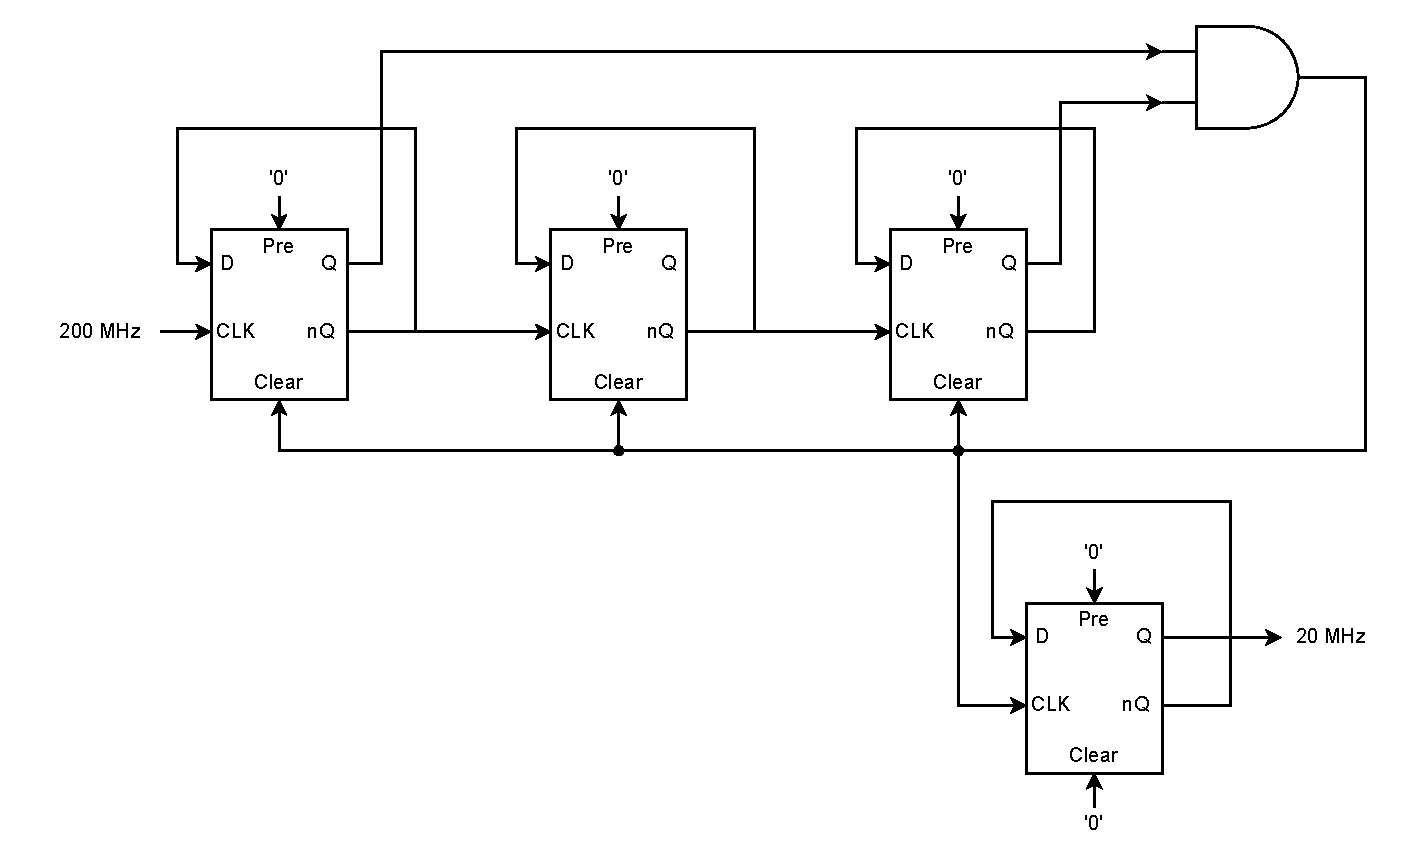
\includegraphics[clip, trim=0 0 0 0, width=1\textwidth]{Sections/7_SystemDesign/Figures/DAC_PRESCALER_LOGIC.pdf}
    \caption{Logic diagram of the DAC prescaler.}
    \label{fig:7_2_3_DAC_PRESCALER_LOGIC}
\end{figure}


The DAC and DDS must be updated not exactly at the same time. This is crucial, as the DAC will update its output to the code present on its data inputs on a rising edge of its clock. The DDS will likewise update its output code on the same edge if they are updated by the same clock. To avoid this, the DAC is clocked by the inverse DDS clock. Thus the DAC is updated \SIQ{180}{\degree} out of phase from the DDS. This will have allowed the DDS data to have settled before the DAC uses it to update its output. A diagram of these signals can be seen in figure \ref{fig:7_2_3_DAC_PRESCALER}.

\begin{figure}[H]
    \centering
    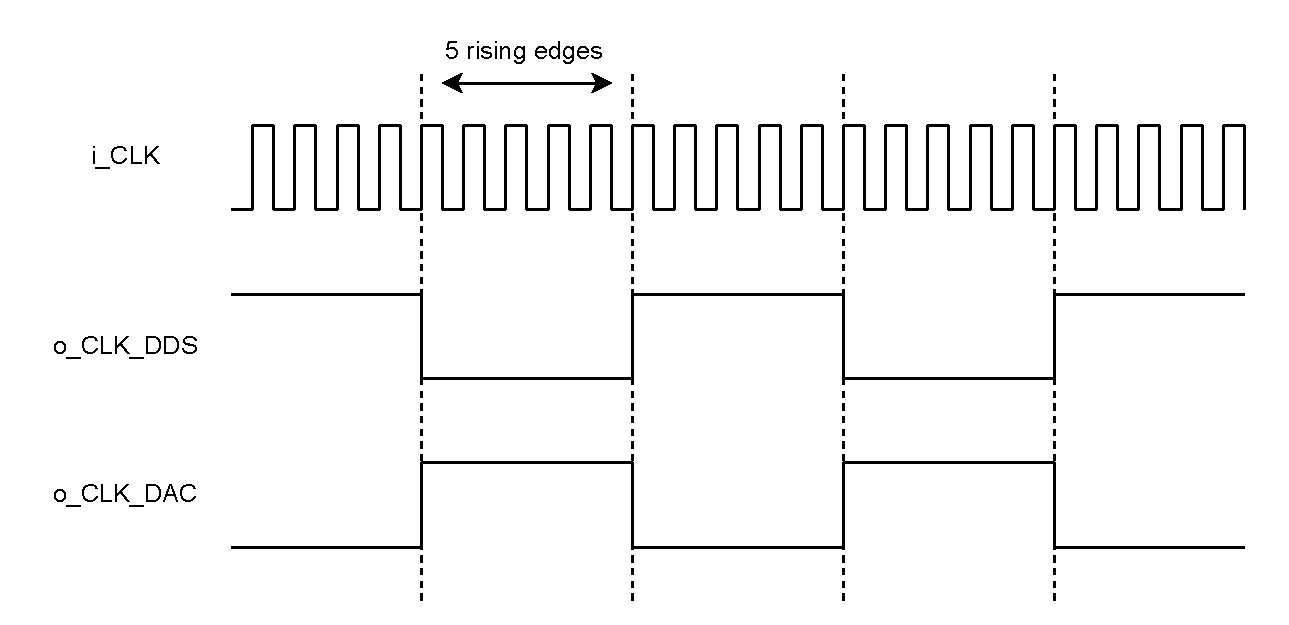
\includegraphics[clip, trim=0 0 0 0, width=1\textwidth]{Sections/7_SystemDesign/Figures/DAC_PRESCALER.pdf}
    \caption{Timing diagram of the input clock and output signals of the DDS and DAC Prescaler.}
    \label{fig:7_2_3_DAC_PRESCALER}
\end{figure}

\subsection*{DAC DATA Conversion}
The DAC DATA Conversion block ensures that the DAC is fed appropriate data and that the DDS block receives the proper 32 bit wide frequency setting word, as well as indicating to the DDS that new data is available for the frequency setting. The VHDL code for the DAC DATA Conversion can be seen in listing \refq{lst:7_2_3_DAC_DATA_Conversion}.

\lstinputlisting[language=c ,style = c,firstnumber=1, linerange=34-70, caption={Code for DAC DATA Conversion}, label={lst:7_2_3_DAC_DATA_Conversion}]{Sections/7_SystemDesign/Code/DAC_DATA_Conversion.vhd}

Lines 3 through 5 in listing \refq{lst:7_2_3_DAC_DATA_Conversion}, shows that it takes in i\_LoByte\_FWORD and i\_LoByte\_FWORD, and puts out o\_FWORD, byte is a bit misleading here as they are 16 bit values. The two inputs are both 16 bit wide busses and the output o\_FWORD is a 32 bit wide bus. Line 21 in the same list shows how the two inputs, i\_HiByte\_FWORD and i\_LoByte\_FWORD, are concatenated to form the 32 bit output bus o\_FWORD.

The DAC DATA Conversion also takes in i\_DDS\_DATA and outputs o\_DAC\_DATA, line 7 and 8 in list \refq{lst:7_2_3_DAC_DATA_Conversion}. Line 24 shows that o\_DAC\_DATA is rather simply i\_DDS\_DATA xor'ed with the hex value "8000" or rather 32768 in decimal. This is the MSB value, and it results in the two's compliment data from the DDS being converted to unsigned values.

To see the effect of xor'ing two's compliment with the MSB, an example of the same operation with a 3 bit variable is shown in table \refq{tab:7_2_3_DAC_DATA_Conversion}. Here it can be seen that the result is that all values are offset by the value of the MSB, in the case of a 3 bit variable, it results in all values being offset by 4, or all values are added a value of 4. 

This is exactly what is desired, as the DAC output should be centered around an offset value, as the DAC cannot output negative values.

\begin{table}[H]
    \begin{tabular}{|l|l|l|l|}
    \hline
    \begin{tabular}[c]{@{}l@{}}A\\ Decimal\end{tabular} & \begin{tabular}[c]{@{}l@{}}A\\ 2's Comp\end{tabular} & B = A xor 100 & \begin{tabular}[c]{@{}l@{}}B\\ Decimal\end{tabular} \\ \hline
    3                                                   & 011                                                  & 111       & 7                                                           \\ \hline
    2                                                   & 010                                                  & 110       & 6                                                           \\ \hline
    1                                                   & 001                                                  & 101       & 5                                                           \\ \hline
    0                                                   & 000                                                  & 100       & 4                                                           \\ \hline
    -1                                                  & 111                                                  & 011       & 3                                                           \\ \hline
    -2                                                  & 110                                                  & 010       & 2                                                           \\ \hline
    -3                                                  & 101                                                  & 001       & 1                                                           \\ \hline
    -4                                                  & 100                                                  & 000       & 0                                                           \\ \hline
    \end{tabular}
    \caption{Example of two's compliment, A, xor'ed with the MSB of a 3 bit integer. The result is in the form of an unsigned integer
    0 having been offset by the value of the MSB.}
    \label{tab:7_2_3_DAC_DATA_Conversion}
    \end{table}

    The process in line 27 trough 37 in listing \refq{lst:7_2_3_DAC_DATA_Conversion} shows how the logic detects if the frequency setting words has been updated. When a rising edge of the i\_CLK here the same clock that drives the DAC, takes place, the input data r\_F\_IN and latched output data r\_F\_OUT are compared, if they are not the same, the logic will set w\_update\_F to high, and update the latched output data to match the input data. On the next rising edge of i\_CLK, the data will be the same, and here w\_update\_F is then set to low again. This creates a pulse the length of the period of i\_CLK, only when new data is present on r\_F\_IN. 
    
    The DDS block will update its output frequency when a rising edge appears on its update frequency input, and thus the DDS will only update its output frequency when new data is present on r\_F\_IN, and r\_F\_IN is generated from concatenating the two memory registers containing the DAC frequency, resulting in the DDS only updating its frequency when the MCU programs in a new frequency to the memory.
\subsection{Sample Memory} \label{subsec:Sample_Memory} 
The Sample Control module will have to store \SIQ{320}{\kilo\bit} of sample data from the ADC before the MCU starts reading them, as mentioned in section \refq{subsubsec:CommunicationDatarate}. The Artix 7 FPGA development\cite{CMOD_A7_AT35T} board being used comes with \SIQ{4}{\mega\bit} of external asynchronous SRAM from ISSI\cite{ISSISRAM} that will be used to store the sampled data. The memory is organized as an array of 512K x 8 bit values, and because the ADC data are 16 bit values the Sample Control module should have hardware to store each sample in two distinct memory addresses in the external memory.

The IS61 SRAM has the functional block diagram shown on figure \refq{fig:7_2_5_IS61Block}.

\begin{figure}[H]
    \centering
    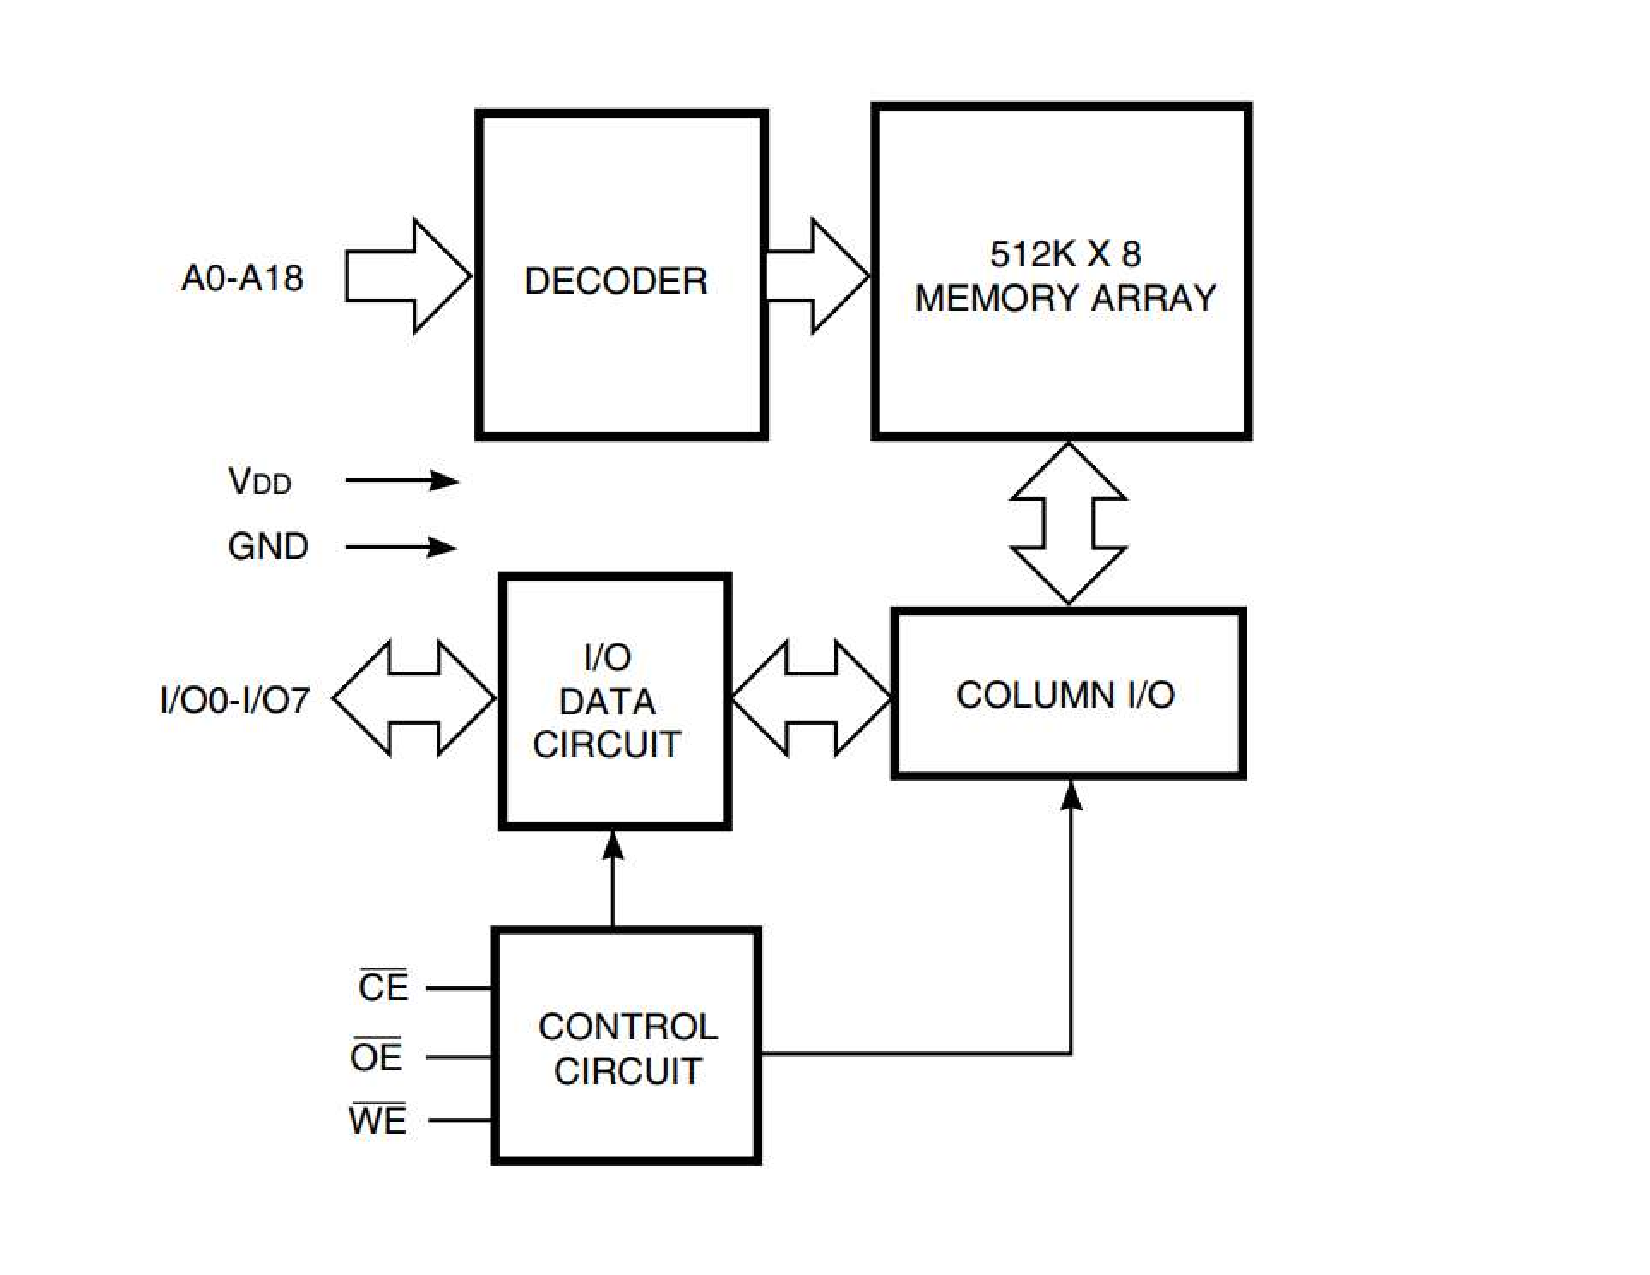
\includegraphics[clip, trim=0 0 0 0, width=0.65\textwidth]{Sections/7_SystemDesign/Figures/7_2_5_IS61_BLOCK_DIAGRAM.pdf}
    \caption{The functional block diagram for the IS61 SRAM\cite{ISSISRAM}. The SRAM uses a 19bit address bus, 8 bit bidirectional data bus along with 3 control signals.}
    \label{fig:7_2_5_IS61Block}
\end{figure}

The FPGA will have to control the address bus, data bus and control signals shown on figure \refq{fig:7_2_5_IS61Block} in order to write to, and read from, the IC. The control signals are Chip Enable (CE), Output Enable (OE) and Write Enable (WE) and they are all active-low signals. The CE input is used to put the the IC into a low-power standby mode, this is not used for this project, so CE is tied to logic '0' at all times. The OE signal controls the state of the output drivers on the chip and a '0' activates the outputs while a '1' sets them into a high impedance state. The WE input controls if a write or read is happening to/from the IC. Note how there is no clock signal, so the memory is asynchronous and any reads, or writes, happens when the WE signal changes state.

In order to write to RAM the FPGA should have hardware that follows the write cycle shown on figure \refq{fig:7_2_5_IS61_WRITE} from the IS61 datasheet.
\begin{figure}[H]
    \centering
    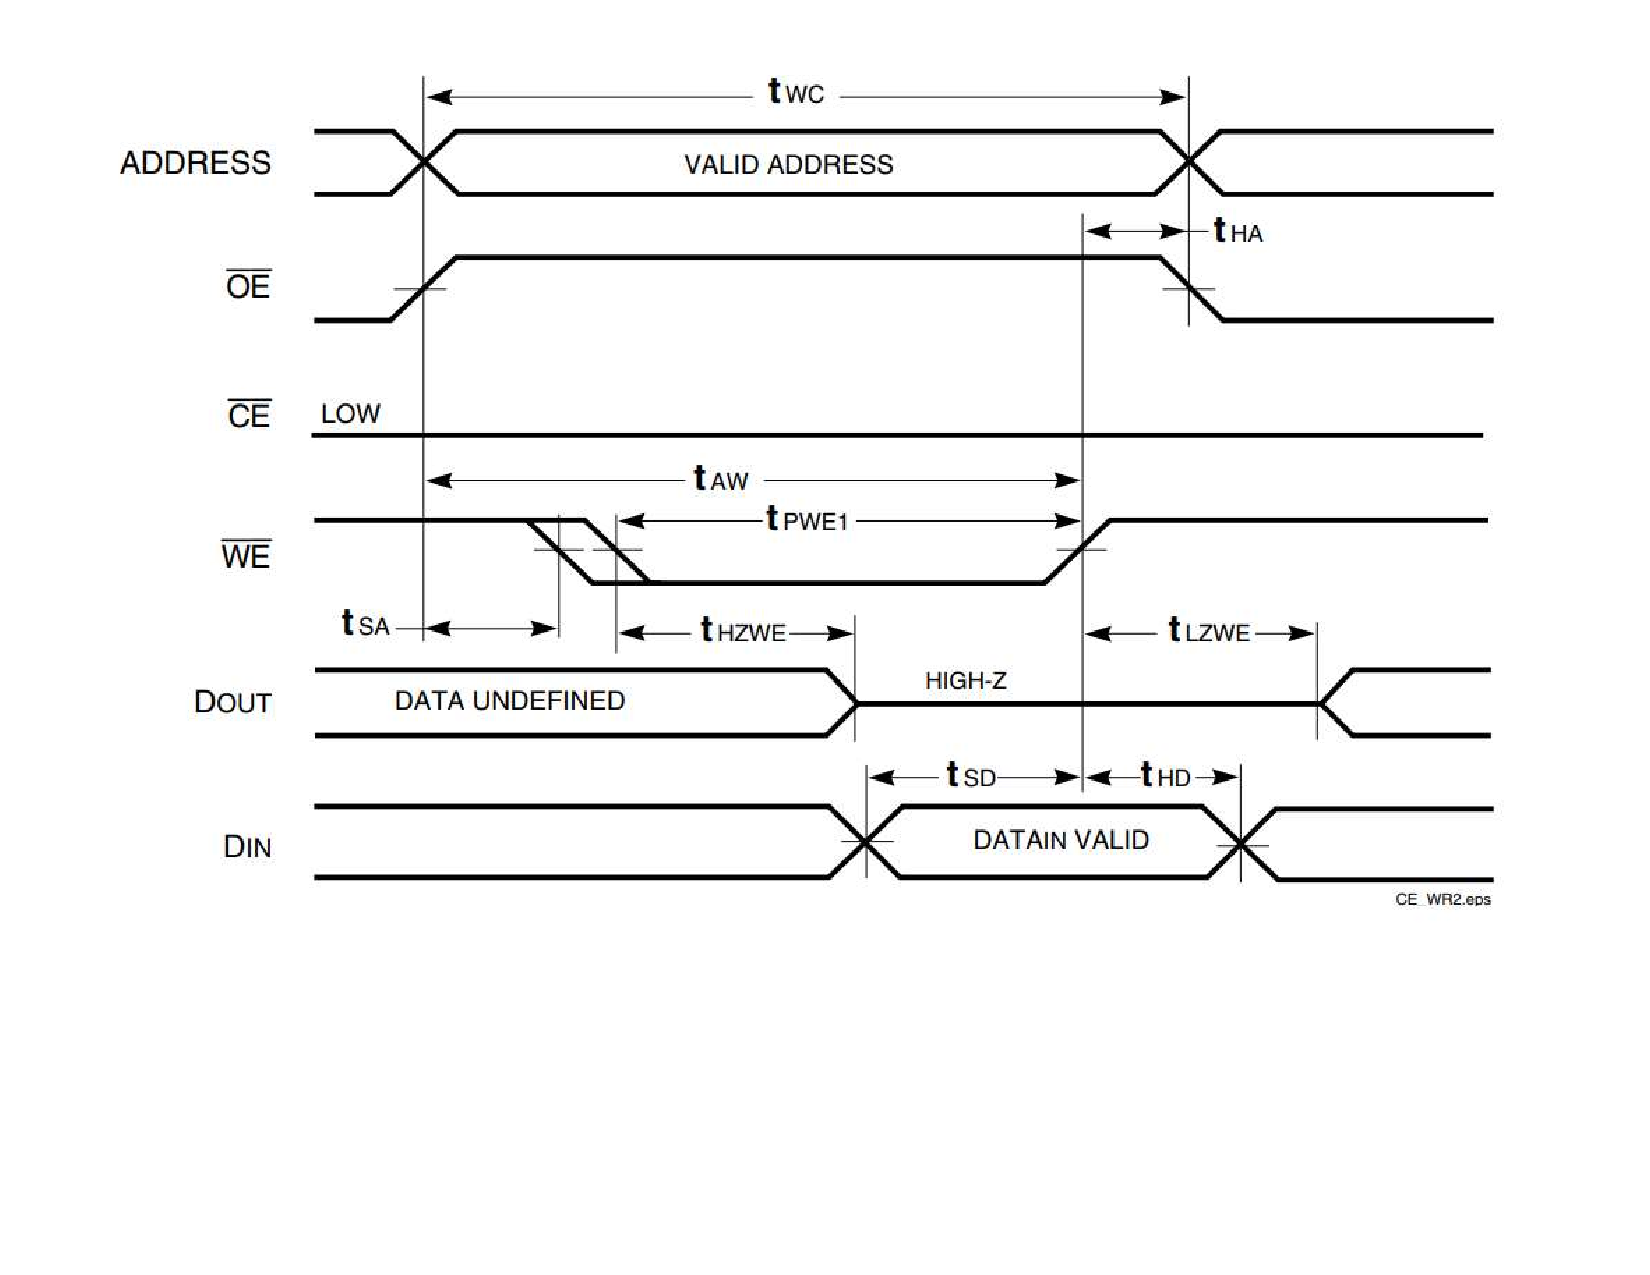
\includegraphics[clip, trim=0 150 0 0, width=0.8\textwidth]{Sections/7_SystemDesign/Figures/7_2_5_IS61_WriteCycle.pdf}
    \caption{A complete write cycle for the IS61 SRAM IC\cite{ISSISRAM}. In order to write to RAM the FPGA should go through the following sequence of events; Set Address to Address bus, Disable output drivers with OE = '1', assert Write Enable with WE = '0', set data to data bus and finish the sequence with WE = '1' to CLK the data byte into RAM.}
    \label{fig:7_2_5_IS61_WRITE}
\end{figure}

The write cycle begins by letting OE go from '0' to '1', the time from this event to WE going low is reffered to as $t_{SA}$ and should be a minimum of \SIQ{0}{\nano\second} according to the datasheet. Figure \ref{fig:7_2_5_IS61_WRITE} does however indicate that the address and OE should be configured before WE goes from '1' to '0'.

the time $t_{HZWE}$ is the time it takes for the output to be tristated after WE goes low, this takes \SIQ{2}{\nano\second} according to the datasheet. Finally there must go at least \SIQ{5}{\nano\second} from the output being tristated to WE going high again, "clocking" in the data on the data IO pins. These time constraints should be repsected for the chip to function properly. All timings are taken for the \SIQ{8}{\nano\second} write cycle chip, this depends on the supply voltage, the memory IC is supplied with \SIQ{3.3}{\volt}, resulting in a write cycle time of \SIQ{8}{\nano\second}, see the datasheet of the IC for more information on this.

The read and write cylces for controlling the memory IC are buid around a counter. If data is to be written or read from the external memory, a counter will increment by 1 at each rising edge of a \SIQ{200}{\mega\hertz} master clock. Depending on the variable of the counter the output of the process will take different states. The advantage of using a counter to advance this state machine is that the timeing constraints can be honored. The VHDL code for the counter can be seen in listing \ref{lst:7_2_5_FSM_COUNTER}. Here it can be seen that if a rising edge on the master clock occurs and the sequence is to run, the counter will increment by 1.

\lstinputlisting[language=C ,style = c,firstnumber=1, linerange=88-93, caption={VHDL code for the FSM counter incrementation.}, label={lst:7_2_5_FSM_COUNTER}]{Sections/7_SystemDesign/Code/EXT_MEM_RW20.vhd}

The write sequence shown on figure \refq{fig:7_2_5_IS61_WRITE} has been implemented in hardware as a state machine as shown in the code listing list \refq{lst:7_2_5_Write_SEQ}.

\lstinputlisting[language=C ,style = c,firstnumber=1, linerange=105-121, caption={VHDL code for the write sequence process.}, label={lst:7_2_5_Write_SEQ}]{Sections/7_SystemDesign/Code/EXT_MEM_RW20.vhd}

When the "v\_Count" is less or equal to 1, this it will be at the first rising edge of the master clock, the address will be set and output enable will be set to a logical '1'. The output data is also set at this point, however the output data is not presented to the IC yet, as a control signal will enable the output buffer at a later state. 

The next rising edge of the master clock will have "v\_Count" take the value 2, and output enable is set to a logical '0'. Here a time of \SIQ{5}{\nano\second} has passend since the last changes due to the period of the master clock being \SIQ{5}{\nano\second}. The time constraint from write enable going low to the data on the datalines being valid is requied to be \SIQ{5}{\nano\second}, to ensure this is honored, two clocks are required to arise before the output buffer is changed from being tristated to being enabled, hence the elsif "v\_Count = 4" statement. Hereafter write enable is set to a logical '1', clokcing in the data. on the next clock the output is once again tristated and the sequence is completed. 

This sequence requires 7 master clocks to be completed and thus it takes \SIQ{35}{\nano\second} to write a single byte to the external memory. This allows for a data-rate of \SIQ{228}{\mega\bit/\second}.

The read cycle for the IS61 SRAM follows a similar procedure as shown on the read cycle timing diagram on figure \refq{fig:7_2_5_IS61_READ}.
\begin{figure}[H]
    \centering
    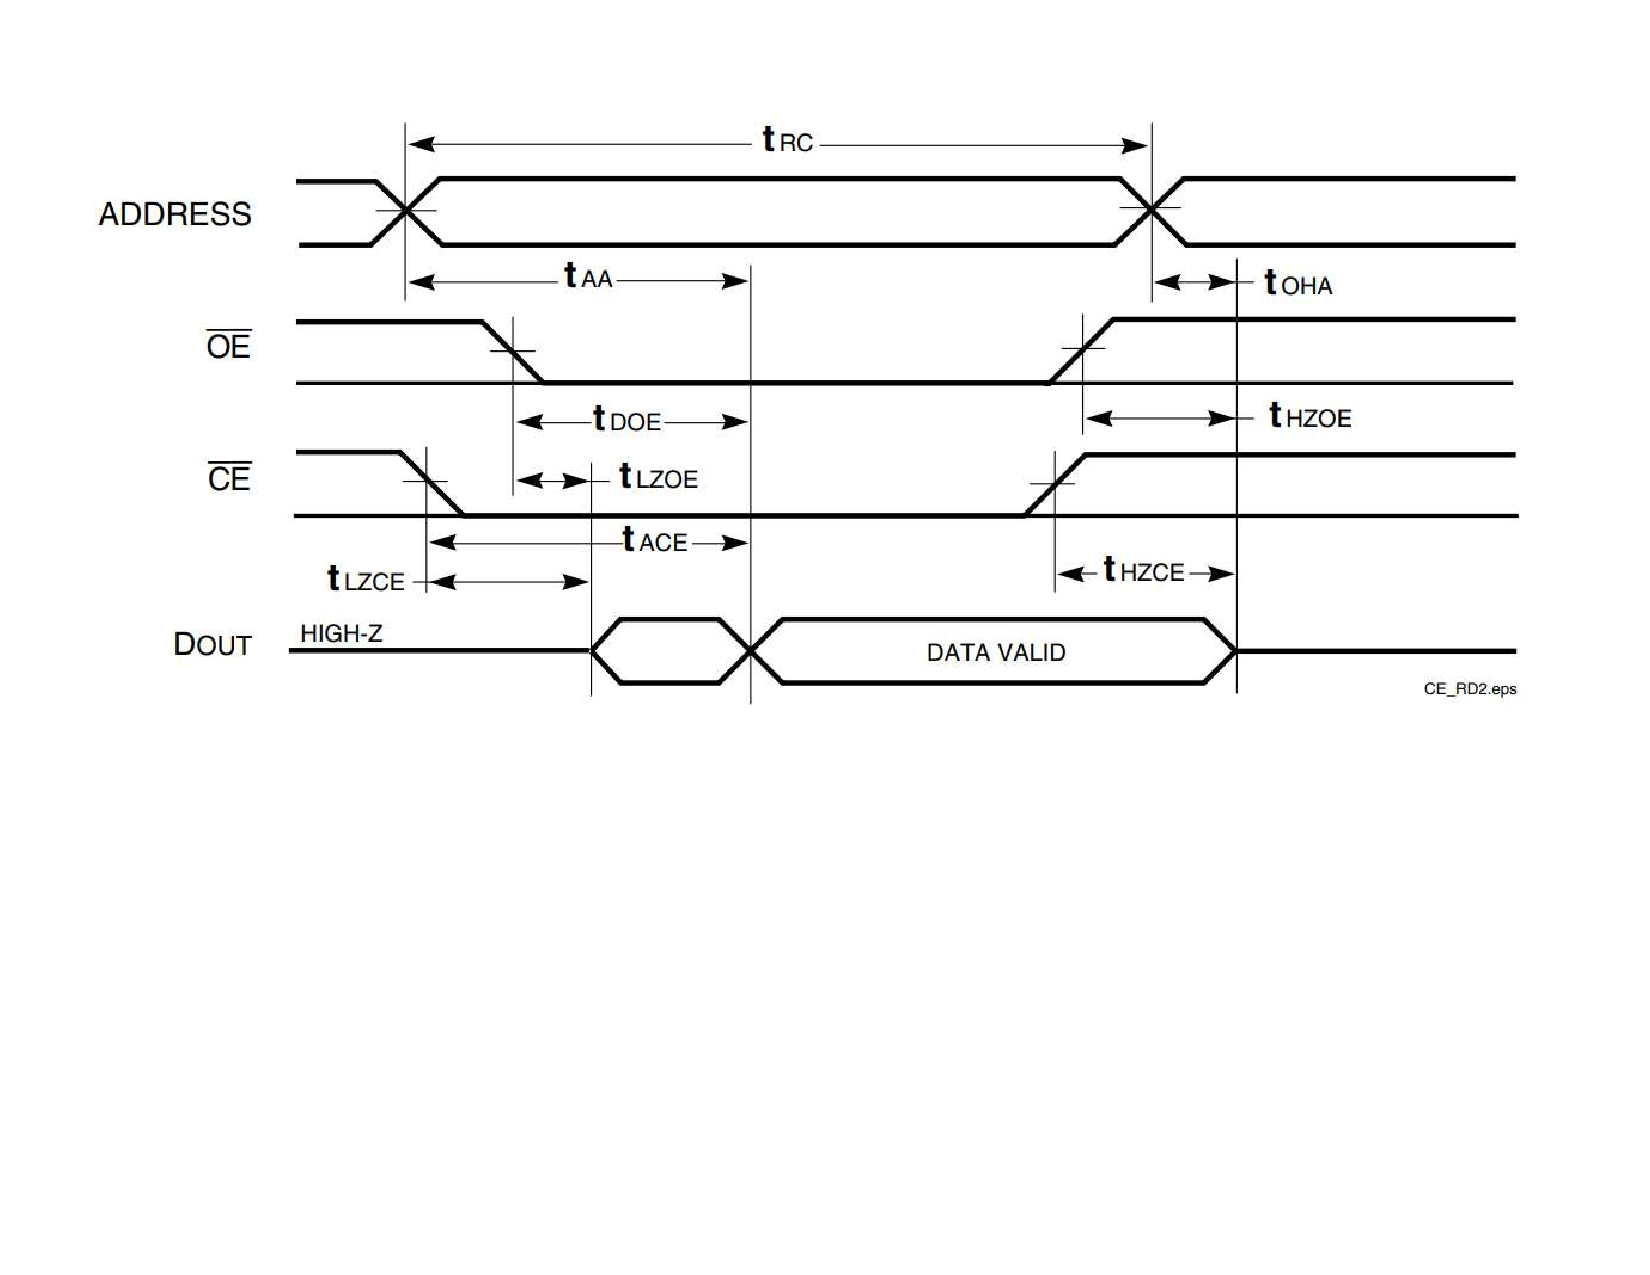
\includegraphics[clip, trim=0 250 0 0, width=0.8\textwidth]{Sections/7_SystemDesign/Figures/7_2_5_IS61_ReadCycle.pdf}
    \caption{A complete read cycle for the IS61 SRAM IC\cite{ISSISRAM}. An address must be set to the address bus, when an address is set the output drivers are enable with OE = '0'. Data is available on the data bus when OE transitions back to OE = '1'. CE is not being controlled in this projects application and is tied to logic '0'.}
    \label{fig:7_2_5_IS61_READ}
\end{figure}

Note how on figure \refq{fig:7_2_5_IS61_READ} the WE signal is not displayed, but WE should be held high for a read cycle in order to work properly. The CE signal is, also, not being controlled in this project and is still tied to '0'. The read cycle is also being controlled by a state machine and the code listing for this can be seen on listing \refq{lst:7_2_5_READ_SEQ}. The time $t_{AA}$ is the time the SRAM uses to fetch the data stored on whatever address is on the address line. With a \SIQ{3.3}{\volt} supply, this time is \SIQ{8}{\nano\second}, this constraint must be respected if proper functionality is to be expected.


\lstinputlisting[language=C ,style = c,firstnumber=1, linerange=94-105, caption={VHDL code for the read sequence state machine}, label={lst:7_2_5_READ_SEQ}]{Sections/7_SystemDesign/Code/EXT_MEM_RW20.vhd} 

The FSM shown in listing \refq{lst:7_2_5_READ_SEQ}  shows that when the sequence is initialized, output enable is set to '0', and a delay of two clocks is then present before the output buffer is tristated, note that the output buffer should already be tristated, but it is forced here as a means of good practice. On the third clock the address that is to be read from is set on the address line. When 6 clocks have occurred, the data on the datalines is latched in on the output data line of the module. The sequence is also set to be complete. This sequence takes 7 clocks to complete aswell or \SIQ{35}{\nano\second}. 

The whole sequence is initialized by the VHDL code shown in listing \ref{lst:7_2_5_start_SEQ}. If "w\_CMPLT" is set to "CMPLT or "i\_RESET" is set to '1', the process will set "w\_RUN" to '0', this will stop the process that Reads/Writes data to the external memory IC. If a rising edge on "i\_EN" arises "w\_RUN" will be set to RUN and the process to Read or Write to the IC will be initialized. Notice also the output "o\_ACTIVE" is "w\_RUN or w\_CMPLT", this results in "o\_ACTIVE" being '1'' for as long as the process is running. Once the process is done reading from or wrtting to the IC, "o\_ACTIVE" will be low. This can be used by other modules to see when the process is complete and new data can be send to this module.

\lstinputlisting[language=C ,style = c,firstnumber=1, linerange=77-86, caption={VHDL code for the read sequence initialization.}, label={lst:7_2_5_start_SEQ}]{Sections/7_SystemDesign/Code/EXT_MEM_RW20.vhd} 

The complete VHDL code for the Sample Memory can be seen in appendix \ref{App:EXT_MEM_RW_CODE}.

\subsubsection{IO Port}
The IO port used is one that can be configured both as an input and an output. A generic component from Xilinx has been used in exaclty the same way as for the FPGA and MCU communication. For more detail on this IO port see section \ref{subsec:Communication}. The signal used to enable or tristate the 8 bit IO datalines to the memory IC is the signal called "o\_IO\_BUF\_CTRL". When this signal is a logical '0' the output buffer is enabled, driving the output.
\subsection{Sample Memory Distribution} \label{subsec:Sample_Memory_Distribution} 
The ADC converters output are 16 bit sample values and the IS61 external SRAM being used in the project can store 8 bit values, so the 16 bit sample values must be mapped into two 8 bit values in order to be stored in the external memory. The function of the Sample Memory Distribution(SMD) submodule is to split the 16 bit word into two bytes and clock it into, and out of, memory through the read/write module described in section \refq{subsec:Sample_Memory}.

For both read and write operations the SMD module will split the incoming 16 bit sample and address into a \textit{high byte} and \textit{low byte} value and map the values to a 17 bit address. The 8 least significant bits will be stored in the address given to the SMD module from the IV Saver module, the 8 most significant bits will be stored in the same address but with address bit 16 set to 1. This allows for $2^{16} = 65536$ addresses to be used, resulting in $65536\cdot16 \approx \SIQ{1}{\mega\bit}$ of sample storage. This does not use the full capability of the memory chip, but it does fullfill the required sample size. 

The SMD module is build as a finite state machine. This FSM is initialized by the VHDL code seen in listing \ref{lst:7_2_6_FSM_INIT}. Here it can be seen that once a rising edge on "i\_SET" occurs, the "w\_init" signal will be set high. This in turn sets the "w\_RUN" signal to RUN on the next rising edge of the \SIQ{200}{\mega\hertz} master clock. Should "i\_RESET = '1'" or "w\_CMPLT = CMPLT" happen the processes will reset and set "w\_init" to '0' and "w\_RUN" to '0'. This way, when the FSM is complete, it sets "w\_CMPLT" to CMPLT, and the process resets itself. Listing \ref{lst:7_2_6_FSM_INIT} also shows that the HiBYTE, LoBYTE, HiADDR and LoADDR are latched in once the process is initialized. This allows the FSM to use the latched registers during its opperation. 

"LoVal" and "HiVal" in listing \ref{lst:7_2_6_FSM_INIT} are "0b000" and "0b001" respectfully, here as binnary values in c linguistics.

\lstinputlisting[language=C ,style = c,firstnumber=1, linerange=117-140, caption={VHDL code to initialize the FSM for the SMD module.}, label={lst:7_2_6_FSM_INIT}]{Sections/7_SystemDesign/Code/MDIST20.vhd} 

Figure \ref{fig:7_2_6_MemDist} shows a diagram of the Sample Memory Distribution FSM. Here "i\_HOLD" is an input from the Sample Memory module. This is the "o\_ACTIVE" signal, and this allows the FSM to "idle" or "halt" until the Sample Memory module is ready to proceed. In write mode, the FSM works simply by setting the output data to the 8 least significant bits of the input data, and the address to the same address as recieved by the IV Saver. It then sets "o\_SET" high indicating to the Sample Memory module that it should save the current data. It then waits for the Sample Memory module to be ready to recieve data again, and repeats this same action but for the 8 most significant bits at their designated address. The Read opperation works in practically the same manor. Notice that there is no Read/Write control, this is due to the Read/Write setting being controlled by the IV Saver, and this RW signal feeds directly through this module and on to the Sample Memory module.

\begin{figure}[H]
    \centering
    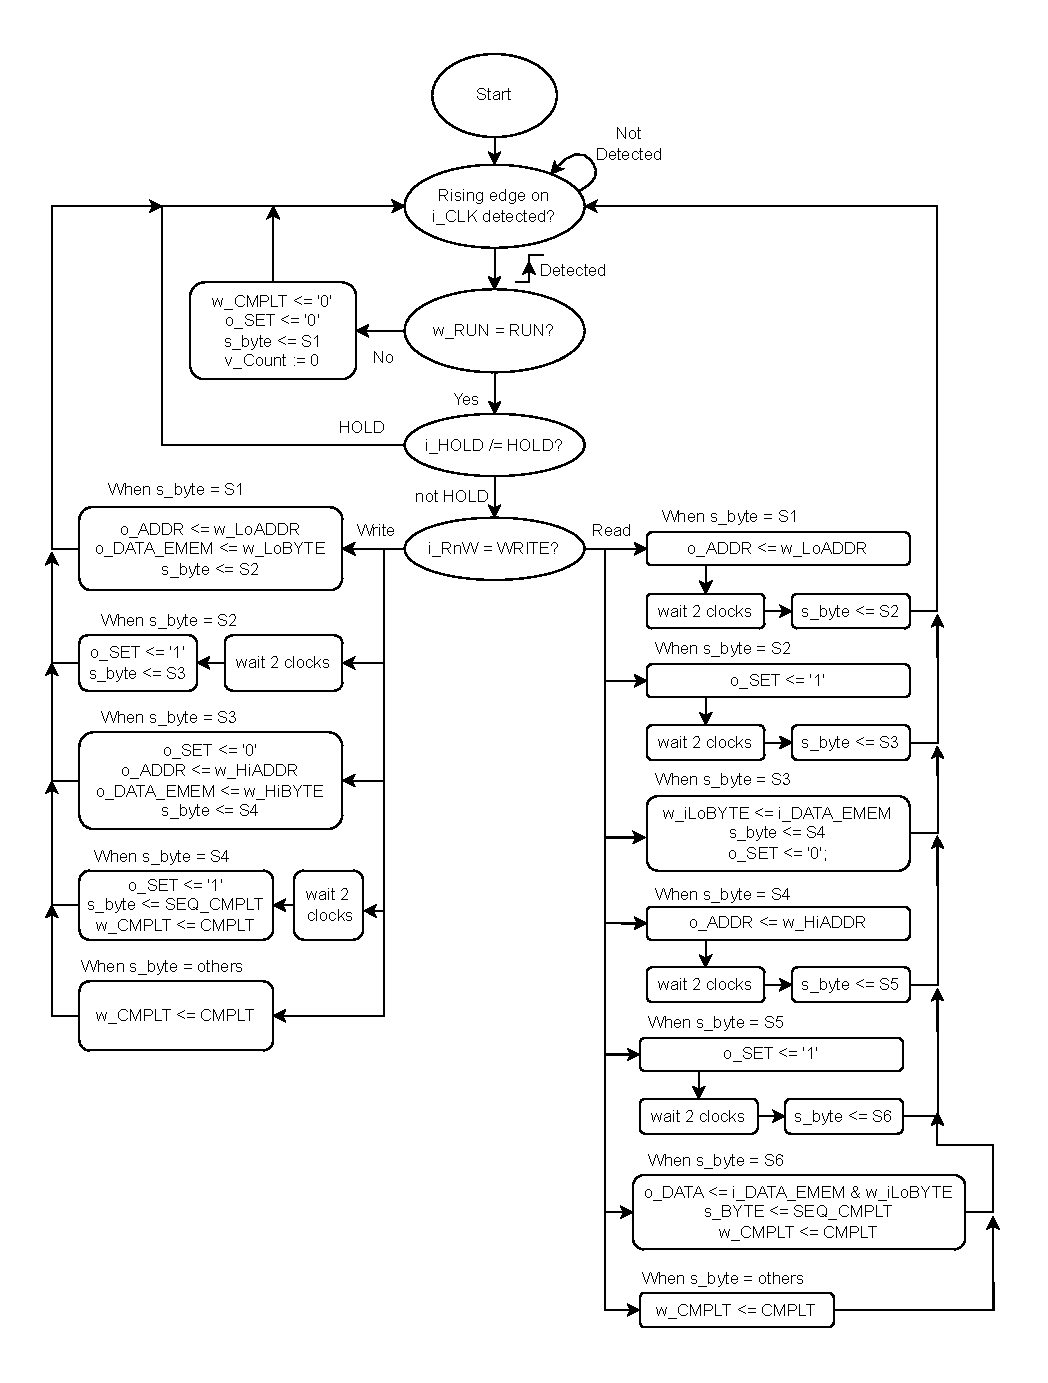
\includegraphics[clip, trim=0 0 0 0, width=1\textwidth]{Sections/7_SystemDesign/Figures/MDIST_FSM.pdf}
    \caption{The module will split an incoming 16 bit word into two bytes and map the address to the 19 bits that the IS61 memory requires.}
    \label{fig:7_2_6_MemDist}
\end{figure}

The SMD module in conjunction with the IV Saver module and Sample Memory module have been tested to reliably save data at a write data-rate of \SIQ{145}{\mega\bit/s}. The SMD module spends roughly \SIQ{80}{\nano\second} to store one 16 bit value. This has been tested by having a busy output for the SMD module. This output consists of the two signals "w\_RUN" and "w\_CMPLT" ored together, this can be seen together with the feedthrough of RW in listing \ref{lst:7_2_6_SMD_BUSY}. The measurements of the output busy flag called "o\_ACTIVE" can be seen appendix in \ref{App:MDIST_BUSY}.

\lstinputlisting[language=C ,style = c,firstnumber=1, linerange=85-87, caption={VHDL code to set RW and output busy flag.}, label={lst:7_2_6_SMD_BUSY}]{Sections/7_SystemDesign/Code/MDIST20.vhd} 
\subsection{ADC Control} \label{subsec:ADC_CONTROL} 

The ADC control block is the controlling hardware for the two external LTC2311\cite{ADC_LTC2311} ADCs that are being used to sample the DUT voltage and current waveforms. The module should, when it sees a rising edge from another HDL block, start a sampling process through the ADCs, clock the data out of the ADCs, latch the data and set a data\_ready flag for the IV saver block to read the sampled data as shown on figure \refq{fig:7_2_8_ADCControlProcess}. This section will only concern itself with the timing of the ADC and the communication between the ADC and FPGA. The complete code for the ADC control module is quite long and can be seen in appendix \refq{App:ADCControlCode}. The code will be explained with diagrams as much as possible. 

\begin{figure}[H]
    \centering
    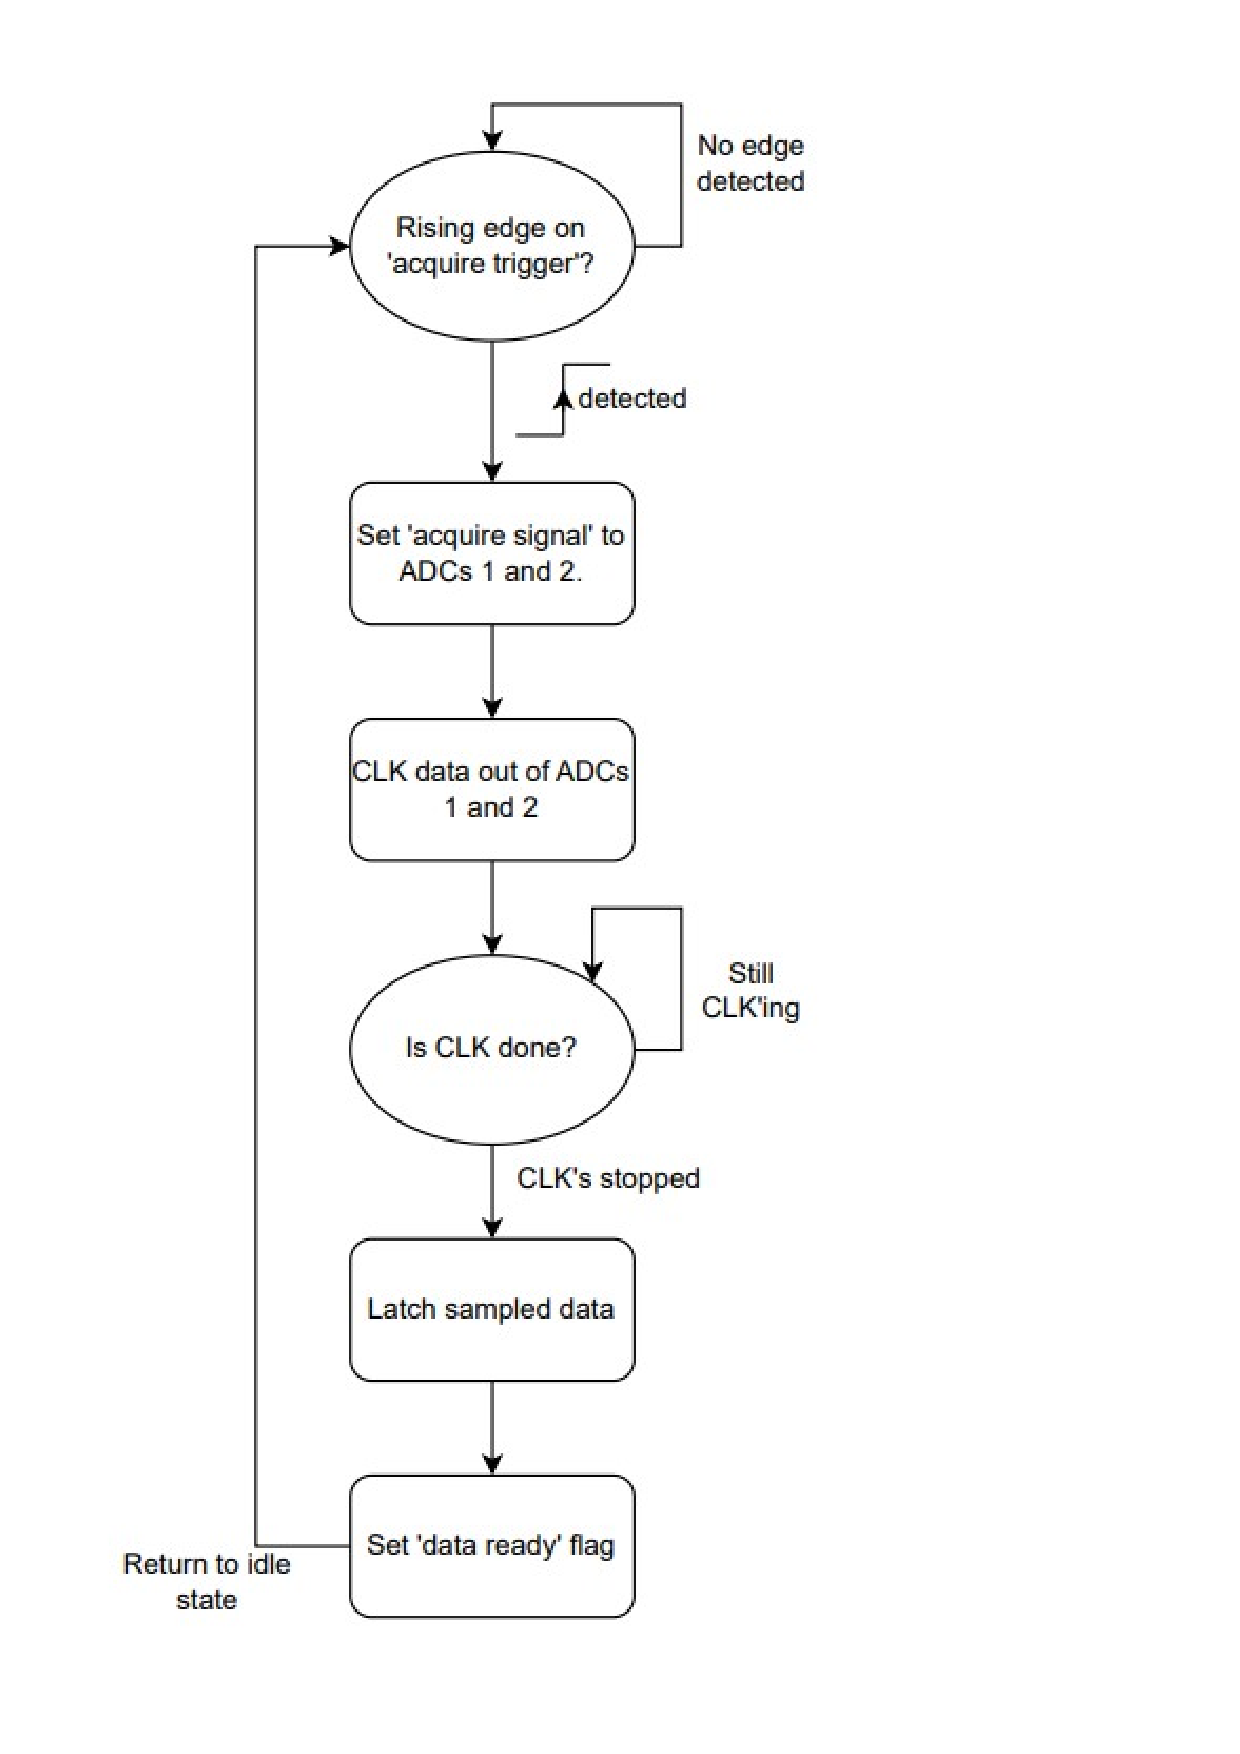
\includegraphics[clip, trim=0 0 0 0, width=0.6\textwidth]{Sections/7_SystemDesign/Figures/7_2_8_ADCControlOverallSignals_cropped.pdf}
    \caption{A process flow showing the overall function of the ADC control block. The block is 'triggered' on a rising edge of an input signal. The block will set an 'acquire' signal to the ADCs, which will start a sample and hold and AD-conversion process. The block will then clock out the sampled data, latch it, and let the next HDL block know that there is sample data ready for processing.}
    \label{fig:7_2_8_ADCControlProcess}
\end{figure}

In order to make the process flow in figure \refq{fig:7_2_8_ADCControlProcess} work the ADC control block must fulfill the timing requirements of the LTC2311 ADC. The timings can be seen on figure \refq{fig:7_2_8_LTC2311_TIMING} where some significant periods have been marked in red on the timing diagram. These will be explained in detail. 

\begin{figure}[H]
    \centering
    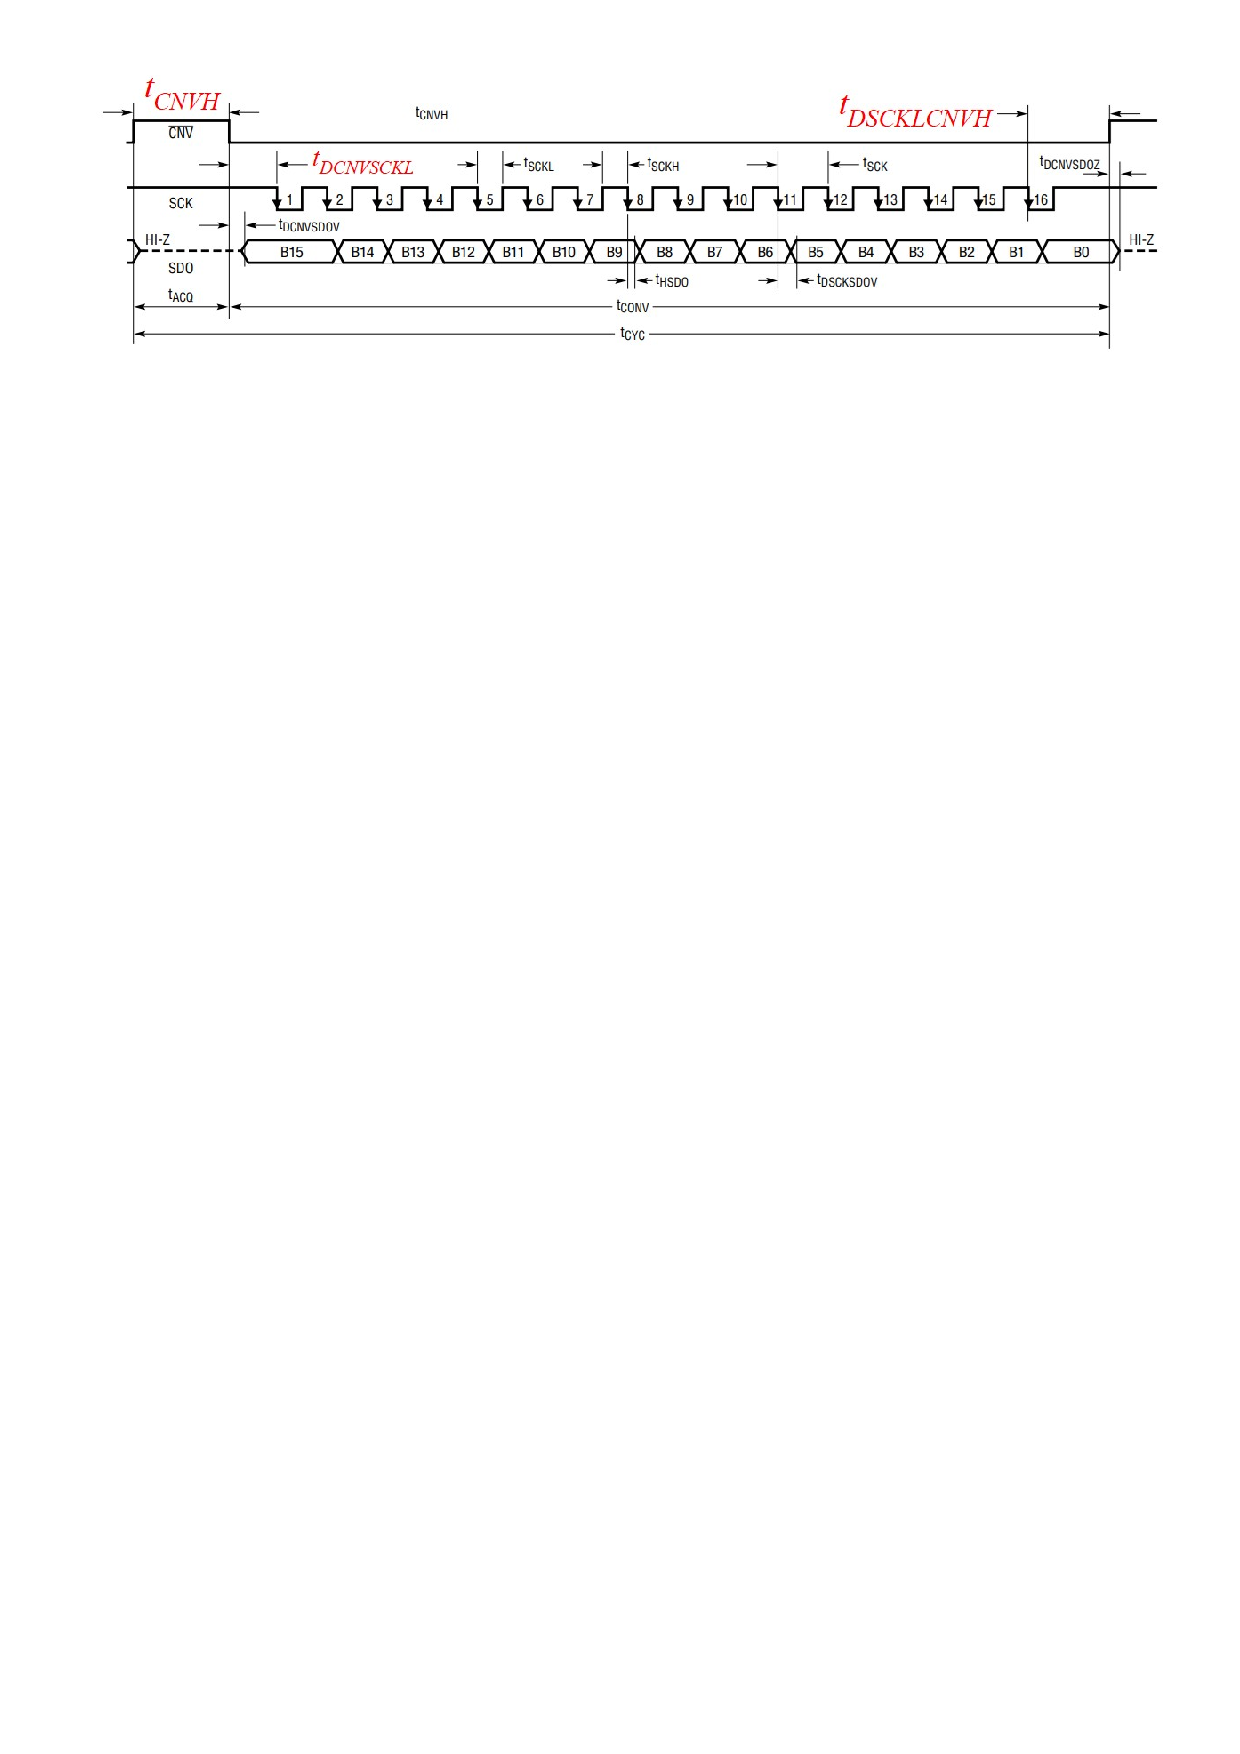
\includegraphics[clip, trim=0 675 0 0, width=1\textwidth]{Sections/7_SystemDesign/Figures/7_2_8_LTC2311_TIMING.pdf}
    \caption{A timing diagram of the communication between the LTC2311 ADC and an SPI master.}
    \label{fig:7_2_8_LTC2311_TIMING}
\end{figure}

The ADC starts an acquisition, i.e. samples the input, when the CNV signal transitions from '0' to '1' and digitizes the value during the $t_{CNVH}$ time. FIgure \refq{fig:7_2_8_LTC2311_TIMING} also lists this time as the acquisition time, $t_{ACQ}$. This time is important and the datasheet suggests $t_{CNVH} = 30 ns$ for a $5M sps$ sample rate. The ADC control block will be designed for a sample rate of $1 Msps$, even though the actual sample rate is expected to be much lower at this point. The main CLK in the sample control module is a \SIQ{200}{\mega\hertz} CLK with a period of $t_{clk} = 5 ns$, so a multiple of this clock period will be convenient for generating the CNV pulse.

The $t_{DCNVSCKL}$ period, marked in red on figure \refq{fig:7_2_8_LTC2311_TIMING}, is the time from a falling edge of CNV to the start of the SPI clock signal. Note how data is clocked out of the ADC on a falling edge of the SPI clock with the MSb being clocked out when the $t_{DCNVSCKL}$ time is passed. The minimum time is listed $t_{DCNVSCKL} = 9.5 ns$ (DCN) in the datasheet. Data is ready and can be clocked into the FPGA on a rising edge of the SPI clock signal as shown on the timing diagram. The $t_{DSCKLCNVH}$ period (DSC), is the minimum time that must pass from the LSb being clocked out of the ADC and until a new CNV pulse can be sent and a new acquisition started. The minimum time for the DSC period is listed as $t_{DSCKLCNVH} = 19.1 ns$.

Assuming $t_{CNV} = 35 ns$, $t_{DCN} = 10 ns$, $t_{DSC} = 20ns$ the SPI clock frequency can be found for a minimum sample rate of $1 MS/s$. The 'protocol' overhead is $t_p = 65 ns$ shown in \refq{eq:7_2_8_ProtocolOverhead}.
\begin{equation}\label{eq:7_2_8_ProtocolOverhead}
        t_{p} = t_{CNV} + t_{DCN} + t_{DSC} = 35e-9 + 10 e-9 + 20 e-9 = 65 e-9
\end{equation}
To get $f_{sample} = 1 MS/s$ with a sample period of $t_{sample} = 1e-6$ and a data packet size of 16 bits equation \refq{eq:7_2_8_SampleFrq} must be true.
\begin{equation}\label{eq:7_2_8_SampleFrq}
   \frac{1}{f_{SPICLK}} \cdot 16 + t_p = t_{sample}
\end{equation}
Using equation \refq{eq:7_2_8_SampleFrq} the sample frequency should, at minimum, be \SIQ{17.11}{\mega\hertz} as shown in equation \refq{eq:7_2_8_SampleFrq2}.
\begin{equation}\label{eq:7_2_8_SampleFrq2}
    f_{SPICLK} = -\frac{16}{t_{p} - t_{sample}} = -\frac{16}{65e-9 - 1e-6} = 17.11e6
 \end{equation}

The minimum SPI clock frequency should be \SIQ{17.11}{\mega\hertz}. This is not a multiple of \SIQ{5}{\nano\second} that the main clock of \SIQ{200}{\mega\hertz} works at. The SPI clock frequency will be set to $f_{SPICLK} = 20 MHz$ as this has a period of $t_{SPICLK} = 1/f_{SPICLK} = 50 ns$ and is a multiple of \SIQ{5}{\nano\second}.

 The ADC control module has been implemented as a state machine whose states will start and stop the various timing pulses required for the SPI communication with the ADCs. The FSM will start when it sees a rising edge of a trigger input signal as shown on figure \refq{fig:7_2_8_ADC_START_ACQ}.

\begin{figure}[H]
    \centering
    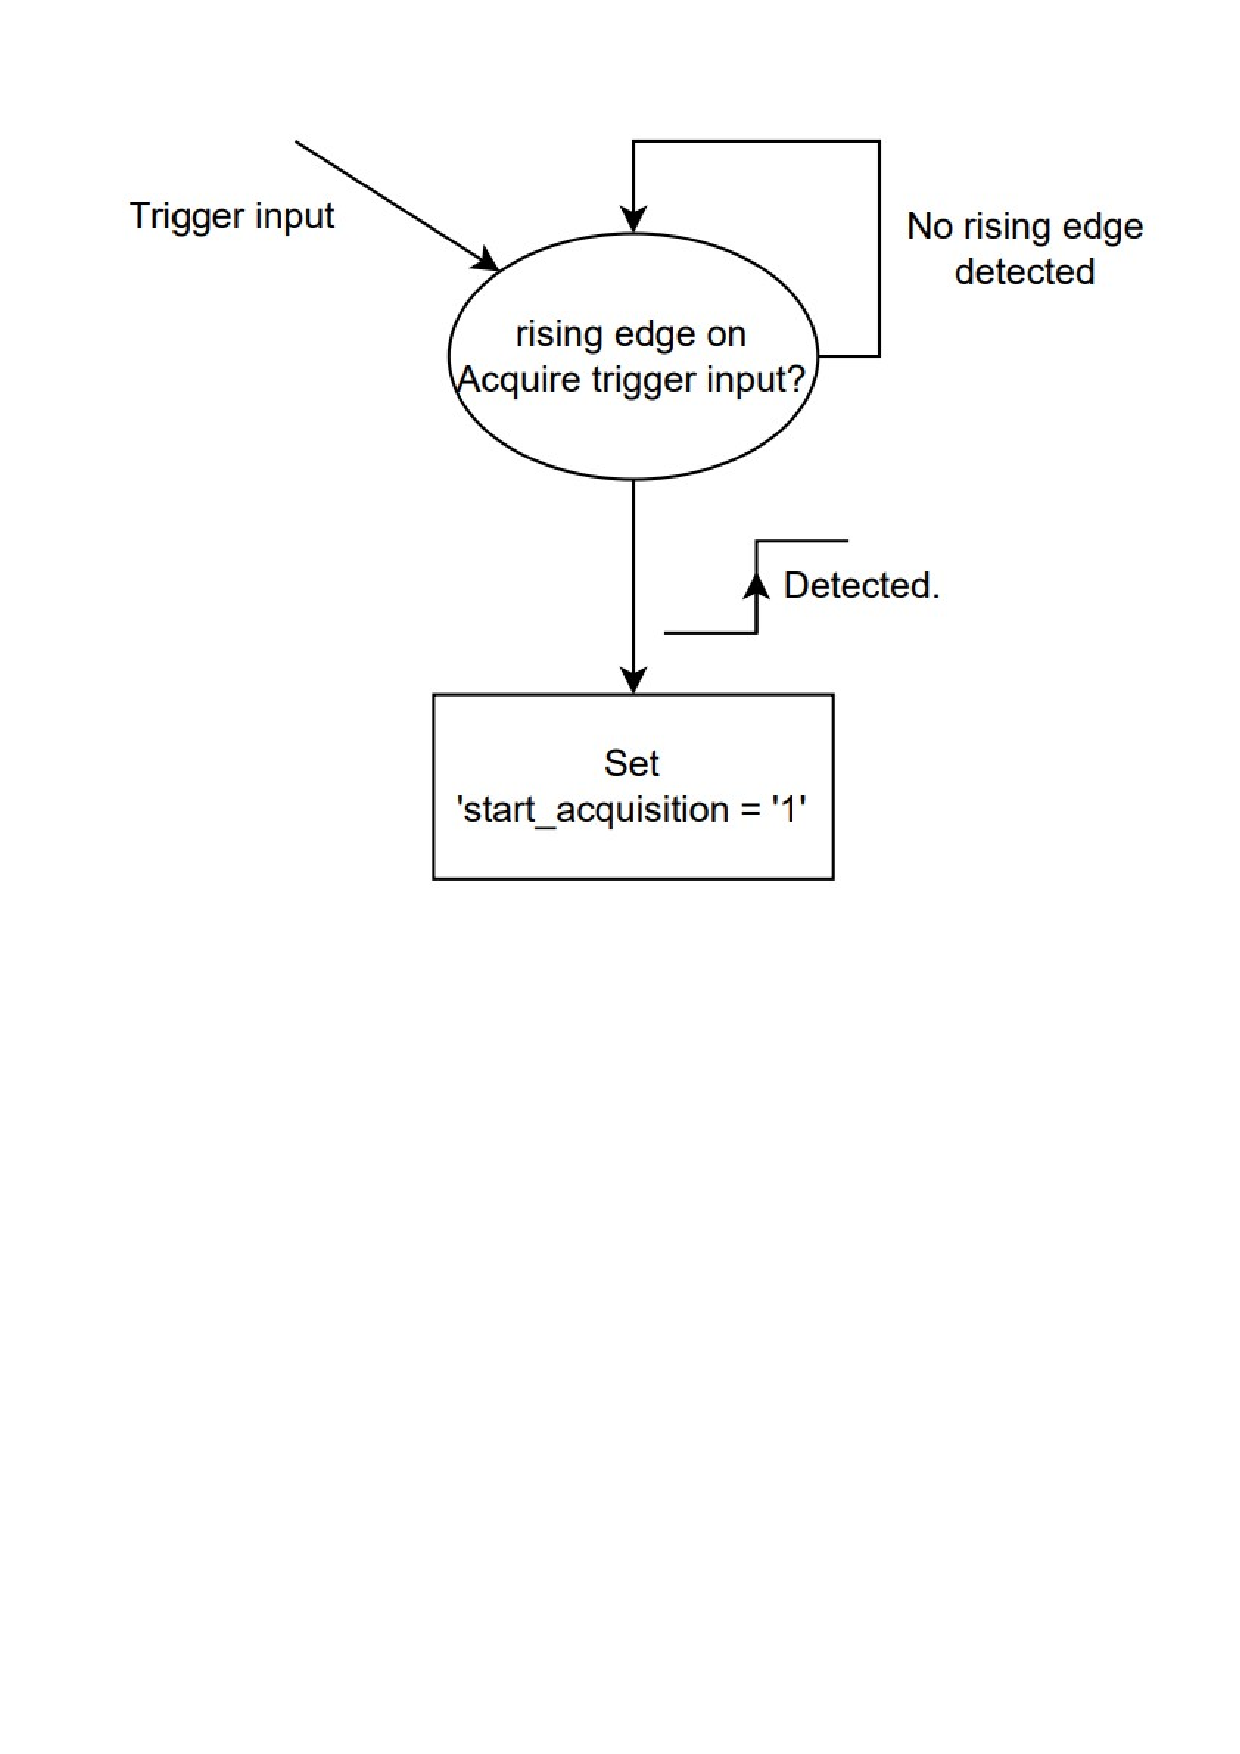
\includegraphics[clip, trim=0 300 0 0, width=0.5\textwidth]{Sections/7_SystemDesign/Figures/7_2_8_StartAcquisition.pdf}
    \caption{A trigger input will signal to the ADC control block that it should enable the FSM that controls the communication with the ADC.}
    \label{fig:7_2_8_ADC_START_ACQ}
\end{figure}

The "start\_acquisition" signal is checked in the FSM and will cause the FSM to start cycling through it's states, starting in the IDLE state and finishing in the LATCH state, as shown on figure \refq{fig:7_2_8_ADC_CONTROL_FSM}.

\begin{figure}[H]
    \centering
    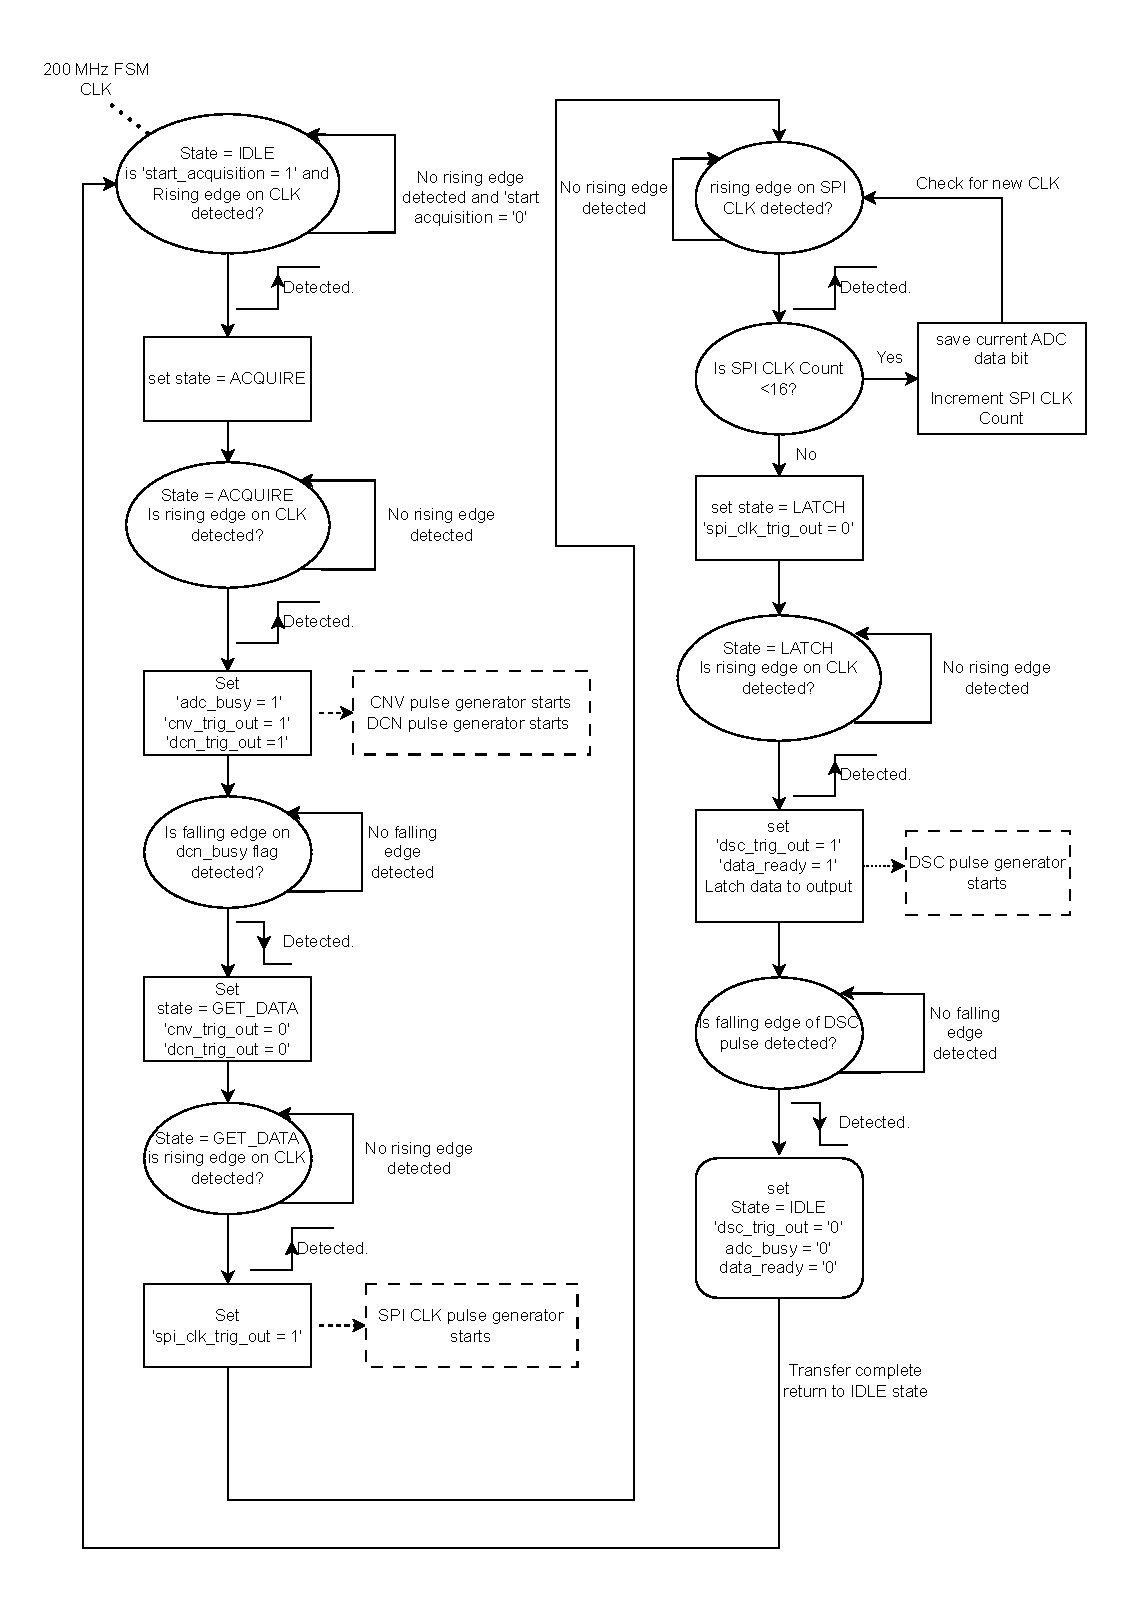
\includegraphics[clip, trim=0 0 0 0, width=0.9\textwidth]{Sections/7_SystemDesign/Figures/7_2_8_ADC Control Logic FSM.pdf}
    \caption{The state machine controlling the timing of the ADC. The FSM is clocked by a 200MHz clock and The FSM starts in the IDLE state in the upper left corner of the figure. The FSM will move from the IDLE state and down through the ACQUIRE and GET\_DATA states before it reaches the LATCH state where it will latch the data it has read from the ADC and return to the IDLE state. The data\_ready flag can be read by the next module in order to see when it should load the data from the ADC control module. The data should be read on a falling edge of the data\_ready flag. Note how the GET\_DATA and LATCH states will start some pulse generators that generate the CNV, DCN and DSC timing signals, these are marked in the dashed boxes. Each of these pulses have "busy" flags that are checked to see when those timing pulses have completed so the FSM can move on, in this way this FSM will generate the timing diagram shown on figure \refq{fig:7_2_8_LTC2311_TIMING}.}
    \label{fig:7_2_8_ADC_CONTROL_FSM}
\end{figure}

As shown on figure \refq{fig:7_2_8_ADC_CONTROL_FSM} the state machine has 4 states, namely IDLE, ACQUIRE, GET\_DATA and LATCH. In the IDLE state the FSM will wait for a trigger input from another module and remain inactive until this happens. When the start\_acquisition signal is asserted the FSM will switch to the ACQUIRE state and, on a rising edge of the master CLK signal, start both the CNV and DCN pulses shown on figure \refq{fig:7_2_8_LTC2311_TIMING}. A rising edge of the CNV pulse is what asserts the sample and hold circuit inside the LTC2311 ADC. The CNV and DCN pulse are generated by instantiations of the pulse generator shown in section \refq{subsec:Pulse_Generator}.

Note how on the timing diagram the DCN pulse is supposed to lag the CNV pulse, and not start at the point in time, this is done on purpose. The DCN pulse will start at the same time as the CNV pulse, but the pulse has the width of the sum of both $t_{CNV} + t_{DCN} = 45 ns$ and the result is that the SPI clock will start at the falling edge of the DCN pulse as desired.  

The various pulse generators used to generate the SPI CLK, CNV, DSC and CVN pulses interface with the ADC control block as shown on figure \refq{fig:7_2_8_PULSE_DELAY_TIMING} and the FSM diagram on figure \refq{fig:7_2_8_ADC_CONTROL_FSM}.

\begin{figure}[H]
    \centering
    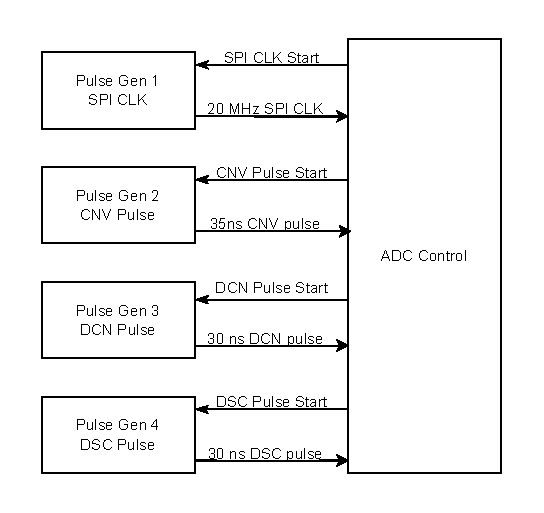
\includegraphics[clip, trim=0 15 0 0, width=0.5\textwidth]{Sections/7_SystemDesign/Figures/7_2_8_PulseAndADCControl.pdf}
    \caption{Various "pulse generators" are used to generate pulses, delays and clock signals in the ADC control module. The SPI CLK is of the type described in section \refq{subsec:PWMGen} and the CNV, DCN and DSC pulses are of the type described in section \refq{subsec:Pulse_Generator}.}
    \label{fig:7_2_8_PULSE_DELAY_TIMING}
\end{figure}

The GET\_DATA state shown on figure \refq{fig:7_2_8_ADC_CONTROL_FSM} will start the SPI CLK pulse generator. This pulse generator is a more advanced version of the pulse generator from section \refq{subsec:Pulse_Generator} and can control the high time and low time pulse widths. This pulse generator will be detailed in section \refq{subsec:PWMGen}. The pulse generator will generate 16 pulses, width a controlled width, that are used to CLK data out of the ADC and into the FPGA. On each falling edge of this CLK a bit is clocked out of the ADC and on the rising edge that same bit is clocked into the FPGA, starting with the MSb. The GET\_DATA state will save the data in a std\_logic\_vector and when it has counted 16 CLKs it will switch state to LATCH.

The LATCH state, will latch the data the FPGA has read when in the GET\_DATA state and signal the next module that it must read the data from the ADC control module. It generates a pulse on the data\_ready signal and data can be read on the falling edge of this signal. The reading module must latch the data before another AD-conversion finishes, or the data is overwritten and lost.

The timing of the ADC module has, of course, been simulated extensively, however it is difficult to show this in this document and the result will vary slightly depending on the actual implementation on the FPGA. The output of the ADC control module has also been verified by use of measurements in order to ensure the correct timing after implementation. A measurement of the acquisition start CNV pulse can be seen on figure \refq{fig:7_2_8_ADC_CONTROL_CNV_MEAS} where the width of the pulse is exactly \SIQ{35}{\nano\second} as expected. 

\begin{figure}[H]
    \centering
    \includegraphics[clip, trim=0 100 0 0, width=0.9\textwidth]{Sections/7_SystemDesign/Figures/7_2_8_ADCControl_CNV_MEASURE.pdf}
    \caption{A measurement of the CNV pulse width. The yellow trace is the CNV pulse. The width is $\Delta X = 35 ns$ as shown in measurement window on the right side of the screen.}
    \label{fig:7_2_8_ADC_CONTROL_CNV_MEAS}
\end{figure}

The DCN time, or, the delay between the falling edge of the CNV pulse and the first falling edge of the SPI CLK signal must be atleast \SIQ{9.5}{\nano\second}, this has also been verified and can be seen on figure \refq{fig:7_2_8_ADC_CONTROL_DCN_MEAS}.

\begin{figure}[H]
    \centering
    \includegraphics[clip, trim=0 150 0 0, width=0.9\textwidth]{Sections/7_SystemDesign/Figures/7_2_8_ADC_CONTROL_DCN_MEAS.pdf}
    \caption{A measurement of the DCN pulse width. The yellow trace is the CNV pulse and the blue trace is the SPI CLK signal. The delay between the falling edge of CNV and falling edge of SPI CLK is $\Delta X = 18.6 ns$ as shown in measurement window on the right side of the screen.}
    \label{fig:7_2_8_ADC_CONTROL_DCN_MEAS}
\end{figure}

The DCN time is slightly longer than the expected \SIQ{15}{ns} due to the actual implementation, but this is OK, a shorter time would not be OK. The SPI CLK frequency has also been verified and can be seen on figure \refq{fig:7_2_8_ADC_CONTROL_SPI_CLK}

\begin{figure}[H]
    \centering
    \includegraphics[clip, trim=0 150 0 0, width=0.9\textwidth]{Sections/7_SystemDesign/Figures/7_2_8_ADC_CONTROL_SPICLK.pdf}
    \caption{A measurement of the SPI CLK frequency. The CLK frequency is 20MHz as shown in the right side of the screen.}
    \label{fig:7_2_8_ADC_CONTROL_SPI_CLK}
\end{figure}

The DSC time has not been verified by measurement, only simulation, instead it has been verified that the ADC control will function at a sample rate of, at least, 1MS/s as was the goal for the module. Several consequtive ADC acquisitions and data transfers can be seen on figure \refq{fig:7_2_8_ADC_CONTROL_1MEGASAMPLE} which proves that the module will work at the desired sample rate as there is no corruption of the communication signals.

\begin{figure}[H]
    \centering
    \includegraphics[clip, trim=0 150 0 0, width=0.9\textwidth]{Sections/7_SystemDesign/Figures/7_2_8_ADC_CONTROL_1MEGSAMPLE_MEAS.pdf}
    \caption{Several consequtive AD-conversions and data transfers. The ADC control module is working as expected at 1 MS/s. The time between the acquisitions can be seen in the right hand side of the screen which shows the frequency of the CNV pulse, and thus sample rate, is 1 MHz.}
    \label{fig:7_2_8_ADC_CONTROL_1MEGASAMPLE}
\end{figure}

As can be seen on figure \refq{fig:7_2_8_ADC_CONTROL_1MEGASAMPLE} the ADC control hardware will work at 1MS/s. There is even time to spare before the next cycle begins. The module can easily be modified to run higher sample rates by adjusting the pulse generators being used in this module, though it may require the use of differential clock and data lines between the FPGA and LTC2311 ADC. The test setup for these measurements, and the measurements themselves can be found in appendix \refq{App:ADCControlMeasurement}.

\subsection{Pulse generator} \label{subsec:Pulse_Generator} 

The ADC control has a need to generate pulses and delays with a specific, accurate, pulse width, so a "pulse generator" module was made. The "pulse generator" module is a module that can be instantiated in an HDL top layer and connected to other blocks in order to generate pulses with a specific pulse width. This pulse generator is a derivation of another module that was used earlier in the project for the same purpose and this can be seen in appendix \refq{App:PulseGenTest}.

The pulse generator will synthesize pulses with a chosen pulse width from the main \SIQ{200}{\mega\hertz} clock with a resolution of $t_{res} = 1/f_{clk} = 1/200E6 = 5ns$, so the shortest pulse it can produce is 5 ns. It is used in the project by instantiating the entity in code \refq{lst:A_PulseGeneratorCode_Entity} in the top layer in the project.

\lstinputlisting[language=C ,style = c,firstnumber=1, linerange=34-43, caption={Entity declaration of the pulse generator}, label={lst:A_PulseGeneratorCode_Entity}]{Sections/7_SystemDesign/Code/pulse_width_gen.vhd}

The width of the pulse is set by the 'width' integer during the time of instantiation and must be a multiple of \SIQ{5}{\nano\second} in order for the module to work. The code for this module is quite simple, so the code will be explained directly. The pulse generator will start by calculating the amount of CLKs it needs to count based on the 'width input as shown in line 8 of listing \refq{lst:A_PulseGeneratorCode_Trigger}.  The pulse generator is asserted by a 'trigger' input signal that is checked with the 'trigger' process in line 10.

\lstinputlisting[language=C ,style = c,firstnumber=1, linerange=47-65, caption={VHDL code for the signals used in the module along with the 'trigger' process.}, label={lst:A_PulseGeneratorCode_Trigger}]{Sections/7_SystemDesign/Code/pulse_width_gen.vhd}

The trigger process will assert the 'r\_start' signal when it sees a rising edge of the trigger input and will be asynchronously reset when the 'r\_done' signal is asserted. The 'r\_done' signal is asserted at the end of a complete pulse as shown in line 12 listing \refq{lst:A_PulseGeneratorCode_PW}.

\lstinputlisting[language=C ,style = c,firstnumber=1, linerange=67-84, caption={VHDL code for the process that generates a pulse of some specified pulse width.}, label={lst:A_PulseGeneratorCode_PW}]{Sections/7_SystemDesign/Code/pulse_width_gen.vhd}

The \texttt{gen\_pulse} process will generate a single pulse of the specified pulse width. When it sees that \texttt{r\_start = 1}, the process will 
set the \texttt{o\_pulse} output pulse signal and synthesize the pulse width from the \texttt{i\_master\_clk} signal by counting the amount of clocks, 
in line 5--6, until it reaches the \texttt{r\_count\_value}, at which point the process will clear the counter and the \texttt{o\_pulse} signal in lines 10-12,
The \texttt{r\_done} flag is set when the counter has finished, and is cleared on the following rising edge of the \texttt{i\_master\_clk} signal.

The pulse generator was tested to see if the generated pulse width matches the one specified in the entity instantiation and, because this pulse generator will generate the CNV pulse for the ADCs, the jitter was also tested. These tests can be seen in appendix \refq{App:PWCPulseGen}. The conclusion is that the pulse generator is suitable for use in the ADC control module.
\subsection{Pulse width modulated pulse generator} \label{subsec:PWMGen} 

This pulse generator is a more advanced version of the generator in section \refq{subsec:Pulse_Generator}. The generator will produce \textit{N} amount of pulses and provides control over the widths of the high and low time of each pulse. The SPI CLK signal used to interface the FPGA to the LTC2311 ADC and described in section \refq{subsec:ADC_CONTROL} requires that the CLK signal is logic high whenever it is not active, so this has also been done with this generator.
The full code for this pulse generator can be seen in appendix \refq{App:PWMGenCode}, but the heart of the generator is two state machines that will be explained in this section.

The pulse generator will generate it's clock pulses based on the MASTER\_CLK input. The CLK could be anything, but it is assumed to be \SIQ{200}{\mega\hertz} in this project and any pulse width will thus be a multiple of the period of a \SIQ{200}{\mega\hertz} signal, which is \SIQ{5}{\nano\second}.

This generator is based on counters for producing accurate 'high' and 'low' periods. The code for generating a single pulse can be seen on listing \refq{lst:7_2_9_PWM_GEN_1_PULSE}.
\lstinputlisting[language=C ,style = c,firstnumber=1, linerange=128-164, caption={VHDL code for generating a single pulse.}, label={lst:7_2_9_PWM_GEN_1_PULSE}]{Sections/7_SystemDesign/Code/pulse_gen_width_modulator_invert.vhd}. 

The process on listing \refq{lst:7_2_9_PWM_GEN_1_PULSE} will generate a single pulse on the on the 'output\_set' signal. If the 'gen\_1\_pulse' signal is asserted and 'pulse\_complete' is cleared then it will proceed to generate a pulse. As can be seen in lines 7 - 27 the generator is a state machine that alternates between a 'HIGH' case and a 'LOW' case. The default case is 'HIGH'.

During the 'HIGH' case; the output is set to '1' and on every rising edge of MASTER\_CLK the counter inside the 'HIGH' case will increment 'clk\_count' in line 11 until it reaches the 'high\_clks' limit. 'high\_clks' is a parameter that can be set during the instantiation of the entity, see appendix \refq{App:PWMGenCode} for the full code. Once the counter has reached the 'high\_clks' value the state will be changes to 'LOW' in lines 12-15 and the process will start timing the 'LOW' period of the output signal.

The 'LOW' case functions exactly like the 'HIGH' case. The output is set to logical '0' and a counter will increment until it reaches the 'low\_clks' value. When it reaches the 'low\_clks' value the state will change back to 'HIGH' and a 'pulse\_complete' signal will be asserted which lets the process in listing \refq{lst:7_2_9_PWM_GEN_SEVERAL_PULSES} know that it it has finished a pulse and is ready for the next one.

\lstinputlisting[language=C ,style = c,firstnumber=1, linerange=91-117, caption={VHDL code for generating multiple pulses}, label={lst:7_2_9_PWM_GEN_SEVERAL_PULSES}]{Sections/7_SystemDesign/Code/pulse_gen_width_modulator_invert.vhd}. 

The VHDL code listing in \refq{lst:7_2_9_PWM_GEN_SEVERAL_PULSES} will, when triggered by an external source, start producing pulses until it reaches the 'NR\_OF\_CLKs' value. When triggered it will assert the 'gen\_1\_pulse' flag and this will start the generation of a single pulse in the way described in listing \refq{lst:7_2_9_PWM_GEN_1_PULSE}. When a single pulse is completed 'gen\_1\_pulse' is released and the process will re-assert 'gen\_1\_pulse' in order to generate another pulse. It continous in this way until the pulse generator has generated 'NR\_OF\_CLKs'.

The pulse generator also has an active/busy signal output that can be used to check if the generator is done pulsing, this can be seen in listing \refq{lst:7_2_9_PWM_GEN_ACTIVE}.

\lstinputlisting[language=C ,style = c,firstnumber=1, linerange=119-126, caption={VHDL code for controlling the active flag.}, label={lst:7_2_9_PWM_GEN_ACTIVE}]{Sections/7_SystemDesign/Code/pulse_gen_width_modulator_invert.vhd}. 

The active flag will set 'active = 1' when the pulse generator gets triggered på an external module. The active flag gets cleared when the pulse generator has reached 'NR\_OF\_CLKs' as seen in line 22 of listing \refq{lst:7_2_9_PWM_GEN_SEVERAL_PULSES}. This module has been tested and these results can be seen in appendix \refq{App:PWMGenTests}.






\subsection{ADC resampler} \label{subsec:ADCResampler}
The ADC resampler block is generating the 'acquire start' (trigger) inputs for the ADC control block. When 'acquire start' for the ADC control module is asserted, the ADC control will start a single conversion. The ADC resampler will generate $N$ amount of trigger pulses for the ADC control block, with $M$ frequency.

The amount of pulses generated, i.e. the sample size $N$, and the sample frequency $M$ along with a 'start' signal is set by a number registers in the internal memory that was described in section \refq{subsec:Memory}. The signals going into, or out of, the ADC resampler can be seen on figure \refq{fig:7_2_10_RESAMPLE_IO}.

\begin{figure}[H]
    \centering
    \includegraphics[clip, trim=0 0 0 0, width=0.9\textwidth]{Sections/7_SystemDesign/Figures/7_2_10_Resample_IO.pdf}
    \caption{A block diagram showing the I/O of the ADC resampler block. The ADC resampler also uses a \SIQ{200}{\mega\hertz} clock and a \SIQ{50}{\mega\hertz} clock, these are not shown on the block diagram.}
    \label{fig:7_2_10_RESAMPLE_IO}
\end{figure}

The module uses a Xilinx Direct Digital Synthesis (DDS) IP\cite{XILINXDDS} to generate the 'acquire start' pulses for the ADC control block. This is a black box component that was described briefly in section \refq{subsec:DAC_CONTROL} and it can be instantiated in an HDL project as a Vivado IP block for signal generation purposes. The output from the DDS module is a two's complement sine wave, but unlike the DAC control block, the ADC resampler block only requires the Numerically Controlled Oscillator portion of the DDS module in order to work, as it uses square waves and doesn't need to make use of the sine loop-up table in the DDS module. The ADC resampler block is getting a square wave from the DDS block by only using the MSb of the sine wave output. The DDS block uses a 48 bit control word, but only 32 bits are used as shown in the entity declaration in listing \refq{lst:7_2_10_ADCResampleEntity}.

\lstinputlisting[language=c ,style = c,firstnumber=1, linerange=37-49, caption={Code for DDS and DAC prescaler}, label={lst:7_2_10_ADCResampleEntity}]{Sections/7_SystemDesign/Code/adc_resampler.vhd}

The two signals, i\_sample\_frq\_low\_int\_mem\_reg and i\_sample\_frq\_high\_int\_mem\_reg, in lines 4 and 5 are concatenated with 0x0000 in order to form a 48 bit frequency control word for the DDS block. The DDS is using a \SIQ{50}{\mega\hertz} clock signal and this gives the DDS output a resolution of \SIQ{17.8}{\micro\hertz} as shown in equation \ref{eq:7_2_10_Fres}.

\begin{equation}\label{eq:7_2_10_Fres}
    f_{res} = \frac{f_{DDSCLK}}{2^N} = \frac{50e6}{2^{48}} = 1.776e-7
\end{equation}
This means the sample frequency of the ADC control block has a resolution of \SIQ{17.8}{\micro\hertz} as well.

The DDS block uses a phase accumulator and the size of the frequency control word affects the output jitter, a larger frequency control word reduces jitter as can be seen in the tests in appendix \refq{App:DDSJitter}. A 48 bit frequency control word is the largest that the DDS module can work with and is thus what is being used in this ADC resampler module.

The ADC resampler has been designed as the mealy machine shown in figure xyz





\section{Sample Control Conclusion} \label{subsec:SampleControlConclusion} 

This is TBD until later.

The Module has these and these speeds... we have tested.. Appendix... the digital system works at sample rates exceeding 2MS/s... etc



%Bibliography
\printbibliography[heading = bibintoc]

%Appendix
\appendix
\chapter{Microcontroller Considerations} \label{App:MicrocontrollerConsiderations}
\chapter{Pin Map: Sample Controller - MCU} \label{App:PinMap_MCU_FPGA}
The specific connections between the MCU (STM32 Nucleo F446RE) and Sample Controller (CMOD A7 Artix-7 35T FPGA) can be seen in this appendix. A block diagram with the specific
connections can also be found. Table \ref{tab:App_MCU_FPGA_PinMap} shows all connections between the MCU and Sample Controller. MCU I.Pin refers to MCU Interface Pin, this is the
pin-number assinged to the connection in the Interface of the MCU, see section \ref{subsec:MainProcessorInterface}. The same is true for FPGA I.Pin, refering to FPGA Interface Pin,
see section \ref{subsec:SampleControlInterface}. A diagram of the connections can be seen in figure \ref{fig_App_MCU_FPGA_PinMap}.

\begin{table}[H]
    \begin{tabular}{|m{5.2em}|m{5.2em}|m{6.7em}|m{6.7em}|m{8.7em}|}
    \hline
    \textbf{MCU I.Pin} &   \textbf{FPGA I.Pin} & \textbf{F446RE Pin} & \textbf{Artix 7 Pin} & \textbf{Reference}  \\ \hline
    0 & 0 & CN7-34/PB0 & GPIO45/U7 & DATA bus 0 \\ \hline
    1 & 1 & CN10-24/PB1 & GPIO44/U3 & DATA bus 1 \\ \hline
    2 & 2 & CN10-22/PB2 & GPIO43/W6 & DATA bus 2 \\ \hline
    3 & 3 & CN10-31/PB3 & GPIO42/U2 & DATA bus 3 \\ \hline
    4 & 4 & CN10-27/PB4 & GPIO41/U5 & DATA bus 4 \\ \hline
    5 & 5 & CN10-29/PB5 & GPIO40/W4 & DATA bus 5 \\ \hline
    6 & 6 & CN10-17/PB6 & GPIO39/V5 & DATA bus 6 \\ \hline
    7 & 7 & CN7-21/PB7 & GPIO38/U4 & DATA bus 7 \\ \hline
    8 & 8 & CN7-38/PC0 & GPIO37/V4 & DATA bus 8 \\ \hline
    9 & 9 & CN7-36/PC1 & GPIO36/W5 & DATA bus 9 \\ \hline
    10 & 10 & CN7-35/PC2 & GPIO35/V3 & DATA bus 10 \\ \hline
    11 & 11 & CN7-37/PC3 & GPIO34/W3 & DATA bus 11 \\ \hline
    12 & 12 & CN10-34/PC4 & GPIO33/V2 & DATA bus 12 \\ \hline
    13 & 13 & CN10-6/PC5 & GPIO32/W2 & DATA bus 13 \\ \hline
    14 & 14 & CN10-4/PC6 & GPIO31/U1 & DATA bus 14 \\ \hline
    15 & 15 & CN10-19/PC7 & GPIO30/T2 & DATA bus 15 \\ \hline
    16 & 16 & CN10-1/PC9 & GPIO47/U8 &  Bus CLK\\ \hline
    17 & 17 & CN10-5/PB9 & GPIO46/W7 & R/$\overline{W}^1$ \\ \hline
    18 & 18 & CN10-2/PC8 & GPIO48/V8 & Bus IX  \\ \hline
    \end{tabular}
    \caption*{
        \raggedright
        $\mathbf{^1}$ $\overline{W}$ is active low. When low the MCU will put data on the BUS.\\
      }
    \caption{Pin map of the interconnections between the MCU and the Sample Controller (FPGA).}
    \label{tab:App_MCU_FPGA_PinMap}
  \end{table}


  
\begin{figure}[H]
    \centering
    \includegraphics[clip, trim=40 130 190 40,width=1.0\textwidth]{Appendix/Figures/FPGA_MCU_PinOut.pdf}
    \caption{Map of the connections between MCU and Sample Controller (FPGA).}
    \label{fig_App_MCU_FPGA_PinMap}
\end{figure}


\chapter{Pin Map: Sample Controller - DAC} \label{App:PinMap_FPGA_DAC}
The specific connections between the Sample Controller (CMOD A7 Artix-7 35T FPGA) and the DAC (LTC1668) can be seen in this appendix. Table \ref{tab:App_FPGA_DAC_PinMap} shows all connections between the DAC and Sample Controller. FPGA I.Pin refers to FPGA Interface Pin, this is the
pin-number assigned to the connection in the Interface of the FPGA, see section \ref{subsec:MainProcessorInterface}. 

\begin{table}[H]
    \begin{tabular}{|m{5.2em}|m{8em}|m{8em}|m{8em}|}
    \hline
    \textbf{FPGA I.Pin} &   \textbf{LTC1668 Pin} & \textbf{Artix 7 Pin} & \textbf{Reference}  \\ \hline
    32 & 14 / DB0 (LSB) & GPIO1 / M3 & DAC Data bit 0 \\ \hline
    33 & 13 / DB1 & GPIO2 / L3 & DAC Data bit 1 \\ \hline
    34 & 12 / DB2 & GPIO3 / A16 & DAC Data bit 2 \\ \hline
    35 & 11 / DB3 & GPIO4 / K3 & DAC Data bit 3 \\\hline
    36 & 10 / DB4 & GPIO5 / C15 & DAC Data bit 4 \\ \hline
    37 & 9 / DB5 & GPIO6 / H1 & DAC Data bit 5 \\ \hline
    38 & 8 / DB6 & GPIO7 / A15 & DAC Data bit 6 \\ \hline
    39 & 7 / DB7 & GPIO8 / B15 & DAC Data bit 7 \\ \hline
    40 & 6 / DB8 & GPIO9 / A14 & DAC Data bit 8 \\ \hline
    41 & 5 / DB9 & GPIO10 / J3 & DAC Data bit 9 \\ \hline
    42 & 4 / DB10 & GPIO11 / J1 & DAC Data bit 10 \\ \hline
    43 & 3 / DB11 & GPIO12 / K2 & DAC Data bit 11 \\ \hline
    44 & 2 / DB12 & GPIO13 / L1 & DAC Data bit 12 \\ \hline
    45 & 1 / DB13 & GPIO14 / L2 & DAC Data bit 13 \\ \hline
    46 & 28 / DB14 & GPIO15 / G2 & DAC Data bit 14 \\ \hline
    47 & 27 / DB15 (MSB) & GPIO16 / J2 & DAC Data 15 \\ \hline
    48 & 26 / CLK & GPIO17 / M1 & DAC CLK \\ \hline
 
    \end{tabular}
    \caption{Pin map of the interconnections between the DAC and the Sample Controller (FPGA).}
    \label{tab:App_FPGA_DAC_PinMap}
  \end{table}

\chapter{Memory Distribution Code} \label{App:MemoryDistributionCode}

This appendix contains the complete code for the memory distribution module.

\lstinputlisting[language=C ,style = c,firstnumber=1, linerange=34-186, caption={VHDL code for the memory distribution}, label={lst:A_MemoryDistributionCode}]{Appendix/Code/ExternalMemoryControl.vhd}
\chapter{Unused Pulse Generator Code } \label{App:UnusedPulseGeneratorCode}

This appendix contains the complete code for the old pulse generator module used in this project.

\lstinputlisting[language=C ,style = c,firstnumber=1, linerange=33-127, caption={VHDL code for the memory distribution}, label={lst:A_PulseGeneratorCode}]{Appendix/Code/pulse_train_gen.vhd}
\chapter{ADC Control Code} \label{App:ADCControlCode}
This appendix has the complete code for the ADC control block code in code list \refq{lst:A_ADCControl} and the top layer required for interfacing the ADC control with the various pulse generators is listing \refq{lst:A_ADCControl_TOP}.

\lstinputlisting[language=C ,style = c,firstnumber=1, linerange=22-249, caption={VHDL code for the ADC control module}, label={lst:A_ADCControl}]{Appendix/Code/adc_control.vhd}

\lstinputlisting[language=C ,style = c,firstnumber=1, linerange=22-312, caption={VHDL code for the ADC control module top layer. The ADC Control takes inputs from several pulse generators in order to fulfill the timing requirement.}, label={lst:A_ADCControl_TOP}]{Appendix/Code/ADC_CONTROL_TOP.vhd}
\chapter{ADC Control Measurements} \label{App:ADCControlMeasurement}
In order to test the ADC control hardware, a PCB has been made that connects the FPGA and LTC2311 ADC. This can be seen on figure \refq{fig:A_ADC_CONTROL_MEAS_SETUP}.

\begin{figure}[H]
    \centering
    \includegraphics[clip, trim=0 100 0 0, width=0.9\textwidth]{Appendix/Figures/A_ADC_CONTROL_MEAS_ADC Control Tesr Setup.pdf}
    \caption{A PCB for testing the ADC Control module. The Artix 7 FPGA, in the middle, is connected to the LTC2311 ADC, in the top. The ADC input is connected to a potentiometer in order to set the voltage it will read. The actual ADC reading can be read on the 16 LEDs in the bottom of the board.}
    \label{fig:A_ADC_CONTROL_MEAS_SETUP}
\end{figure}

The board in the middle is the CMOD A7 Artix 7 development board being used in the project. The connections to the FPGA is not interesting as all FPGA pins can be used as GPIO, so, any pins can be chosen here. While the green board in the top is a break out board for the LTC2311 ADC that was designed for this project. The schematic for this breakout board can be seen on figure \refq{fig:A_ADC_CONTROL_LTC2311SCH}

\begin{figure}[H]
    \centering
    \includegraphics[clip, trim=0 0 0 0, width=1\textwidth]{Appendix/Figures/A_ADC_CONTROL_LTC2311SCH.pdf}
    \caption{The schematic for the LTC2311 ADC Breakout board that was designed for this project.}
    \label{fig:A_ADC_CONTROL_LTC2311SCH}
\end{figure}

Note how the LTC2311 is being used in "CMOS" mode as can be sen on figure \refq{fig:A_ADC_CONTROL_LTC2311SCH}. This means the communication for the LTC2311 is single ended. Setting the CMOS/LVDS mode changes the LTC2311 to LVDS mode which means the SCK and SDO signals will be in differential mode.

The BNC connector on figure \refq{fig:A_ADC_CONTROL_MEAS_SETUP} is an input that can be used as a manual, external, trigger input for the ADC control block. The LEDs on the bottom can be used to see an actual reading from the ADC. The accuracy of the readings are not interesting here as the module only controls the timing and communication between the LTC2311 and the FPGA.

The signal going to the CNV pin has been measured and can be seen on figure \refq{fig:A_ADC_CONTROL_CNV}.

\begin{figure}[H]
    \centering
    \includegraphics[clip, trim=0 75 0 0, width=1\textwidth]{Appendix/Figures/A_ADCControl_CNV_MEASURE.pdf}
    \caption{A measurement of the pulse width of the CNV pin signal. The pulse width is \SIQ{35}{\nano\second} as expected. The yellow trace is CNV. The purple trace is ADC data and the blue trace is SPI CLK.}
    \label{fig:A_ADC_CONTROL_CNV}
\end{figure}

The CNV to CLK signal dead time has been measured and can be seen on figure \refq{fig:A_ADC_CONTROL_DCN}.

\begin{figure}[H]
    \centering
    \includegraphics[clip, trim=0 150 0 0, width=1\textwidth]{Appendix/Figures/A_ADC_CONTROL_DCN_MEAS.pdf}
    \caption{A measurement of the dead time between the falling edge of the CNV pin signal and the start of the SPI CLK. The dead time is about \SIQ{18.6}{\nano\second} which is OK for this project.  The yellow trace is CNV. The purple trace is ADC data and the blue trace is SPI CLK.}
    \label{fig:A_ADC_CONTROL_DCN}
\end{figure}

The pulse widths of the SPI CLK signals have been measured and this can be seen on figure \refq{fig:A_ADC_CONTROL_SPICLKWIDTH}.
\begin{figure}[H]
    \centering
    \includegraphics[clip, trim=0 150 0 0, width=1\textwidth]{Appendix/Figures/A_ADC_CONTROL_PULSEWIDTH.pdf}
    \caption{A measurement of pulse widths of the SPI CLK pulses can be seen. Both the high and low time is about \SIQ{25}{\nano\second} as was expected for this.  The yellow trace is CNV. The purple trace is ADC data and the blue trace is SPI CLK.}
    \label{fig:A_ADC_CONTROL_SPICLKWIDTH}
\end{figure}

The SPI CLK frequency can also be seen on figure \refq{fig:A_ADC_CONTROL_SPICLKWIDTH} and is \SIQ{20}{\mega\hertz}. It was checked whether the ADC control can do 1 MS/s and this test can be seen on figure \refq{fig:A_ADC_CONTROL_1MSS}.

\begin{figure}[H]
    \centering
    \includegraphics[clip, trim=0 150 0 0, width=1\textwidth]{Appendix/Figures/7_2_8_ADC_CONTROL_1MEGSAMPLE_MEAS.pdf}
    \caption{A test of the ADC control block running at 1 MS/s. There are no glitches in the communication so the hardware works at 1 MS/s. The yellow trace is CNV. The purple trace is ADC data and the blue trace is SPI CLK.}
    \label{fig:A_ADC_CONTROL_1MSS}
\end{figure}
\chapter{Pulse Generator Measurements} \label{App:PulseGenTest}
It was necessary to make a more advanced version with absolute control over the pulse width of the pulses, as the first pulse of the simpler pulse generator in section \refq{subsec:Pulse_Generator} will sometimes make short, initial, pulses as it works entirely by gating the main clock and is subject to variations in pulsewidths depending on when, exactly, the generator is started relative to the main clock, this can cause violations of the LTC2311 timing. This variation in the pulse widths can be seen on figure xyz where the output of the simple pulse generator has been measured.
%INDSÆT BILLEDE af perspective view
\chapter{Pulse Width Modulated Pulse Gen Code} \label{App:PWMGenCode}
This appendix has the full code listing for the Pulse Generator with Pulse Width Modulation \refq{lst:A_PWM_GEN_CODE}.

\lstinputlisting[language=C ,style = c,firstnumber=1, linerange=23-184, caption={VHDL code for generating a single pulse.}, label={lst:A_PWM_GEN_CODE}]{Appendix/Code/pulse_gen_width_modulator_invert.vhd}. 
\chapter{Pulse width modulated pulse generator measurements} \label{App:PWMGenTests}

\chapter{Pulse width controlled pulse generator} \label{App:PWCPulseGen}
This appendix presents a VHDL pulse-generator capable of generating different pulse-widths.

The pulse width generator that was described in section \refq{subsec:Pulse_Generator} has been tested.

First, the pulse width of the output was tested. The default pulse width of the module is 40ns and is set in line 3 of code listing \refq{lst:A_PulseGeneratorCode_Entity}. This is the pulse width that will be tested.

\lstinputlisting[language=C ,style = c,firstnumber=1, linerange=34-43, caption={Entity declaration of the pulse generator}, label={lst:A_PulseGeneratorCode_Entity}]{Sections/7_SystemDesign/Code/pulse_width_gen.vhd}

The pulse generators 'o\_pulse' output is connected to an FPGA output pin and the 'i\_master\_clk' signal is a \SIQ{200}{\mega\hertz} CLK signal. The 'i\_trigger' input is connected to a \SIQ{1}{\mega\hertz} internal CLK. The output of the pulse generator can be seen on figure \refq{fig:A_PulseGenWidth_WidthTest}.

\begin{figure}[H]
    \centering
    \includegraphics[clip, trim=0 50 0 50, width=1\textwidth]{Appendix/Figures/A_PulseWidthGen_PulseWidth.pdf}
    \caption{An oscilloscope screenshot of the pulse generators output a long with the trigger input. The yellow signal is the trigger input and the purple signal is the pulse generators output. With \SIQ{10}{\nano\second} per division the pulse width is \SIQ{40}{\nano\second} as expected.}
    \label{fig:A_PulseGenWidth_WidthTest}
\end{figure}

The jitter of the pulse generator has also been verified. To do this the trigger input and pulse generator output was measured with an oscilloscope. The oscilloscope is a Rigol DHO924S and it was set to use one of it's 'deep memory' functions, called Ultra Acquire, in order to display several waveforms side by side. The pulse generator is set to produce 40 ns pulses and the results of this can be seen on figure \refq{fig:A_PulseGenWidth_JitterTest}.

\begin{figure}[H]
    \centering
    \includegraphics[clip, trim=0 50 0 50, width=1\textwidth]{Appendix/Figures/A_PulseGen_Test.pdf}
    \caption{An oscilloscope screenshot of the pulse generators 'trigger' input (yellow) and 'pulse' output(red). The oscilloscope is using a deep memory 'ultra acquire' mode to display 20 consequtive readings in a 'mosaic' pattern.}
    \label{fig:A_PulseGenWidth_JitterTest}
\end{figure}

It can be seen that, unlike the old pulse generator seen in appendix \refq{App:PulseGenTest}, there appears to be no visible, or varying, delays between the pulse generators activation and the pulse output.

The jitter was measured in another way as well. The pulse generator is set to be retriggered continously, and, since it is expected that the ADC control will take up to 20000 samples at a maximum sample rate of 1MS/s, a delay was added to the oscilloscope in order to see the jitter after 20ms have passed. This delay can be seen on figure \refq{fig:A_PulseGenWidth_JitterTestA}.

\begin{figure}[H]
    \centering
    \includegraphics[clip, trim=0 50 0 50, width=1\textwidth]{Appendix/Figures/A_PulseWidthGen_JitterA.pdf}
    \caption{The oscilloscope settings used to measure the jitter. A 20ms delay is added ot the oscilloscope trigger in order to see the 20000th pulse relative to the first pulse.}
    \label{fig:A_PulseGenWidth_JitterTestA}
\end{figure}

Setting the oscilloscope to use maximum persistence it is possible to see the amount of jitter at the 20000th pulse. The result of this can be seen on figure \refq{fig:A_PulseGenWidth_JitterTestB}.

\begin{figure}[H]
    \centering
    \includegraphics[clip, trim=0 50 0 50, width=1\textwidth]{Appendix/Figures/A_PulseWidth_Gen_JitterB.pdf}
    \caption{A measurement of the jitter of the output of the pulse generator. It is measurably <\SIQ{1}{\nano\second} after 20000 cycles.}
    \label{fig:A_PulseGenWidth_JitterTestB}
\end{figure}

There is little jitter as can be seen on figure \refq{fig:A_PulseGenWidth_JitterTestB}. The oscilloscope is set to \SIQ{2}{\nano\second} per division and the jitter is less than half a division, so, <\SIQ{1}{\nano\second}. This pulse generator can be used for generating CNV pulses.

\chapter{ADC Control 2 MS/s} \label{App:HSADCControlTest}
This appendix shows the considerations for the set sampling rate of the system.

The working principle for the sampling system was decided early on in the project, and the highest test frequency that has to be measured is \SIQ{1}{\mega\hertz} sine waves. The choice was between two principles, either the project samples at 2MS/s in order to adhere to the Nyquist sampling theorem, or a sub-sampling principle is used. Sub-sampling is where the anti-aliasing effect is exploited in order to sample the waveforms at lower sample rates. Ultimately it was decided to use the sub-sampling principle over concerns of signal fidelity on the physical PCB and uncertainties and memory data rates. The clock signals for the ADCs would have to be \textit{high} and high frequency square waves pose certain challenges that the project team doesn't have enough time to solve for this semester project. The digital system in the sample control module is designed to operate at higher sample rates than is actually used, so that the project can be switched to use the higher 2MS/s sample rates if the team wants to switch sampling principle, so this was also tested for the ADC control module.

The only change that the module requires in order to do this, is to change the SPI CLK frequency since all the other pulses, such as CVN, DCN and DSC as described in section \refq{fig:7_2_8_ADC_CONTROL_DCN_MEAS} are already designed for higher sample rates. The ADC control module uses the pulse generator from section \refq{subsec:PWMGen} to make the SPI CLK and simply changing the values of the 'HIGH' and 'LOW' period changes the SPI CLK frequency. This has been done in this 2 MS/s test.

On figure \refq{fig:A_HighSpeedADCControlTest_CNV} it can be seen that the distance between the CNV pulses, in yellow, is \SIQ{480}{\nano\second}. There is some error in this measurement due to manual cursor placement on the oscilloscope. This corresponds to a CNV frequency of \SIQ{2.083}{\mega\hertz} as shown on the right side of the screen.
\begin{figure}[H]
    \centering
    \includegraphics[clip, trim=0 75 0 50, width=0.9\textwidth]{Appendix/Figures/A_HighSpeedADCControlTestCNV.pdf}
    \caption{A measurement of the CNV frequency. The sample rate of the ADCs is equal to the CNV pulse frequency. Yellow is the CNV pulse, blue is the SPI CLK and red is the SPI data bus.}
    \label{fig:A_HighSpeedADCControlTest_CNV}
\end{figure}

The fidelity of the SPI CLK signal was of special interest so this was also measured on it's own. The results can be seen on figure \refq{fig:A_HighSpeedADCControlTest_SPICLK}

\begin{figure}[H]
    \centering
    \includegraphics[clip, trim=0 75 0 50, width=0.9\textwidth]{Appendix/Figures/A_HighSpeedADCControlTestSPICLK.pdf}
    \caption{A measurement of the SPI CLK. With the modifications to the pulse generator that was described in this appendex, the SPI CLK frequency is 50MHz. Yellow is the CNV pulse, blue is the SPI CLK and red is the SPI data bus.}
    \label{fig:A_HighSpeedADCControlTest_SPICLK}
\end{figure}

The SPI CLK shown on figure \refq{fig:A_HighSpeedADCControlTest_SPICLK} is ,almost, more triangular shaped than it is a square wave, and quite noisy. There are various reasons for this. The oscilloscope input and probes are loading the SPI CLK bus, the SPI CLK is a single-ended signal and the FPGA may not be quite capable of driving the bus on it's own. Using the higher sample rate requires more time than is available for the project, to gain enough confidence in these high speed signals to implement it in practice, so the sub-sampling principle is used.
\chapter{Direct Digital Synthesis Jiter} \label{App:DDSJitter}
The DDS IP was tested in order to see how different settings affect output jitter. The only difference in these tests is the length of the frequency control word. The input clock signal is a \SIQ{50}{\mega\hertz} clock signal.

The system is expected to take 10000 samples and with a sample frequency of \SIQ{1}{\mega\hertz} this means the last sample will be taken \SIQ{10}{\milli\second} after the initial acquisition. All the measurements are taken with a \SIQ{20}{\milli\second} delay in order to see an absolute worst case in the sample jitter, note how this is twice the expected sample size. The output of the DDS module for a 32 bit frequency control word can be seen on figure \refq{fig:A_DDS_JITTER_32BIT}.

\begin{figure}[H]
    \centering
    \includegraphics[clip, trim=0 50 0 0, width=0.9\textwidth]{Appendix/Figures/A_DDS_JITTER_32BIT.pdf}
    \caption{A measurement of the output jitter from the DDS block using a 32 bit frequency control word. There is \SIQ{20.48}{\nano\second} of output jitter as can be seen in the measurements in the right side of the screen.}
    \label{fig:A_DDS_JITTER_32BIT}
\end{figure}

The output of the DDS module for a 48 bit frequency control word can be seen on figure \refq{fig:A_DDS_JITTER_48BIT}.
\begin{figure}[H]
    \centering
    \includegraphics[clip, trim=0 50 0 0, width=0.9\textwidth]{Appendix/Figures/A_DDS_JITTER_48BIT.pdf}
    \caption{A measurement of the output jitter from the DDS block using a 48 bit frequency control word. There is \SIQ{1.862}{\nano\second} of output jitter as can be seen in the measurements in the right side of the screen.}
    \label{fig:A_DDS_JITTER_48BIT}
\end{figure}

Clearly, a larger control word gives better output jitter performance. Note how the output is allowed to "settle" for about 30 seconds before the oscilloscope snapshot was taken. It was noted that the jitter of the 48 bit control word will also grow in size if it is allowed to run for an extended period of time, but a larger control word offers higher performance in the short term in all cases and is thus better for the sampling system.
\chapter{Resampler VHDL code} \label{App:ResamplerCode}

This appendix contains the full code for the ADC resampler block. The code can be seen in listing \refq{lst:A_Resampler_Code}.

\lstinputlisting[language=c ,style = c,firstnumber=1, linerange=22-251, caption={VHDL Code for the ADC Resampler}, label={lst:A_Resampler_Code}]{Appendix/Code/adc_resampler.vhd}
%input{Appendix/GIT}




\end{document}
